\documentclass[14pt]{extreport}
\usepackage{listings}
\usepackage[english]{babel}
\usepackage[utf8]{inputenc}
\usepackage{amsmath}
\usepackage{graphicx}
\usepackage{textcomp}
\usepackage{qtree}
\usepackage[colorinlistoftodos]{todonotes}
\usepackage {tikz}
\usetikzlibrary {positioning}
%\usepackage {xcolor}
\definecolor {processblue}{cmyk}{0.96,0,0,0}
\usepackage{listings}
\lstset{language=C, tabsize=4, mathescape}
\usepackage{tikz}
\usetikzlibrary{calc,shapes.multipart,chains,arrows}
\usepackage{mathtools}
\usepackage{geometry}
\geometry{legalpaper, margin=0.6in}
\usepackage{float}
\def\codefont{
  
  \fontsize{13pt}{13pt}\selectfont}
\definecolor{codebgcolor}{HTML}{EDEDED}
\newenvironment{code}
{\begin{center}
    \begin{tikzpicture}
      \node [fill=codebgcolor,rounded corners=5pt]
      \bgroup
      \bgroup\codefont
      \begin{tabular}{l}}
      {\end{tabular}
      \egroup
      \egroup;
    \end{tikzpicture}
  \end{center}}


\title{Algorithm Engineering}

\author{Luca Corbucci}

\date{\today}

\begin{document}
\maketitle

\tableofcontents

\chapter{Lezione 1}

\section{Definizione di algoritmo}

Nel libro "The Art of Computer Programming" Donald Knuth definisce un algoritmo come "una procedura finita, definita, effettiva con alcuni output". Nel dettaglio:
\begin{itemize}
    \item Finita: l'algoritmo deve terminare sempre dopo un numero ragionevole di passaggi. Il termine "ragionevole" (rispetto alla difficoltà del problema) è legato all'efficienza dell'algoritmo;
    \item Definito: ogni step dell'algoritmo deve avere un significato preciso e non ambiguo, se lo legge un'altra persona non deve avere una "interpretazione" diversa dalla nostra;
    \item Effettivo: tutte le operazioni effettuate nell'algoritmo devono essere abbastanza semplici da poter essere eseguite anche con carta e penna.
\end{itemize}

\section{Un nuovo modello}

Un algoritmo va analizzato per capire il tempo e lo spazio necessario per la sua esecuzione, il modello basilare che si è considerato fino a qualche anno fa è il "RAM Model" (1 CPU + 1 Memoria) in cui ogni accesso alla memoria costa $O(1)$ e il tempo necessario $T(N)$ lo calcoliamo considerando il numero di operazioni che vengono svolte dall'algoritmo. Spazio e tempo dipendono dalla $n$ in input, maggiore è n e più aumentano gli step necessari per l'esecuzione dell'algoritmo (e quindi il tempo), allo stesso modo aumentano anche le celle di memoria occupate durante l'esecuzione dell'algoritmo (e quindi lo spazio necessario).
Dati due algoritmi analizzati con il modello RAM è possibile confrontarli per capire quale dei due è migliore dal punto di vista del tempo necessario all'esecuzione.

Il modello RAM attualmente non è più utilizzato (se non in teoria) e si è passati ad un modello più complicato in cui abbiamo più di una CPU e una gerarchia di memoria. L'accesso alla memoria ha un costo differente a seconda di dove si trova la memoria all'interno della gerarchia, alla cache si accede in poco tempo (nanosecondi), al disco si accede in un tempo che è nell'ordine dei millisecondi. 
Per risolvere questo problema di "I/O Bottleneck" o si cerca di trovare soluzioni hardware o si migliorano gli algoritmi, spesso migliorando gli algoritmi si ottiene una soluzione migliore rispetto al miglioramento dell'hardware.
Ad esempio, consideriamo 3 algoritmi con 3 costi differenti in termini di tempo necessario per l'esecuzione:
\begin{itemize}
    \item $C_1(n) = n$: se abbiamo un tempo massimo $t$ e ogni operazione di $I/O$ costa c, i dati su cui possiamo lavorare sono al massimo $n*c = t$ ovvero $n = \frac{t}{c}$. Se aumentiamo il tempo di k, la quantità di dati scala perfettamente di un fattore k. $n = \frac{t*k}{c}$.
    \item $C_2(n) = n^2$: se abbiamo un tempo massimo $t$ e ogni operazione di $I/O$ costa c, i dati su cui possiamo lavorare sono al massimo $n^2*c = t$ ovvero $n = \sqrt{\frac{t}{c}}$. Se aumentiamo il tempo di k, la quantità di dati diventa. $n = \sqrt{\frac{t*k}{c}}$.
    \item $C_3(n) = 2^n$: se abbiamo un tempo massimo $t$ e ogni operazione di $I/O$ costa c, i dati su cui possiamo lavorare sono al massimo $2^n*c = t$ ovvero $n = log(\frac{t}{c})$. Se miglioriamo l'hardware e il tempo aumenta di k, la quantità di dati non scala. $n = log(\frac{t*k}{c})$.
\end{itemize}

Quindi il miglioramento dell'hardware non sempre porta un miglioramento in termini di tempo necessario per l'esecuzione degli algoritmi e molto spesso è preferibile avere un algoritmo migliore.

\section{Un primo problema: sommare gli elementi di un array}

Consideriamo il problema di dover sommare tutti gli n elementi di un array.
Banalmente possiamo scorrere l'array e sommare in una variabile i vari elementi, eseguiamo n somme.
Possiamo generalizzare questo approccio considerando un modo differente di accedere agli elementi dell'array, consideriamo infatti due parametri b = dimensione del blocco logico dell'array tale che per ogni blocco $[0,n/b]$ abbiamo che il blocco j comprende gli elementi $A_j = A[j*b+1,(j+1)*b]$ e s = numero di salti da fare verso destra una volta letto un elemento dell'array, s deve essere coprimo con $n/b$ perchè altrimenti andiamo a vedere sempre gli stessi blocchi. Otteniamo un modello $A_{s,b}$ per l'accesso ai dati dell'array, indipendentemente dai parametri s e b, da un punto di vista computazionale, tutti l'algoritmo ha sempre lo stesso costo perchè leggiamo sempre n interi, la differenza ce l'abbiamo in quanto ad efficienza se la dimensione n dell'array cresce perchè quando cresce n ed aumentano i dati da sommare, questi saranno distribuiti su tanti livelli di memoria e quindi avremo un costo maggiore per accedere ai vari livelli. Se ad esempio abbiamo D dischi e in ogni disco vogliamo accedere ad una pagina di memoria di dimensione B allora leggeremo un totale di $D*B$ elementi provenienti da D dischi differenti.
Per migliorare l'efficienza dell'algoritmo nel momento in cui si accede ai dati in memoria quindi devono essere sfruttate principalmente due feature:
\begin{itemize}
\item Località spaziale: se accedo il blocco I è probabile che poi accederò anche il blocco I+1; 
\item Località temporale: se ora accedo ad un certo blocco, è probabile che lo accederò di nuovo a breve.
\end{itemize}

Analizziamo l'algoritmo $A_{s,b}$ considerando un array di n elementi, dei blocchi logici nell'array di b elementi e delle pagine di memoria grandi B.
\begin{itemize}
\item Consideriamo $A_{1,1}$ quindi abbiamo pagine logiche grandi 1 elemento e saltiamo ogni volta di 1, quindi in pratica scorriamo l'array. L'algoritmo svolge $\frac{n}{B}$ operazioni di I/O.
\item Prendiamo il caso in cui $b<B$ e s = 2 ovvero ogni volta saltiamo un elemento del blocco b. Se ad esempio abbiamo b=2 e B=4 vuol dire che ogni volta consideriamo solamente due elementi del blocco B quindi poi è necessario caricare due volte il blocco in memoria per accedere di nuovo agli elementi che non abbiamo ancora visto.
Quindi le operazioni di I/O diventano in questo caso $\frac{2*n}{B}$.
\end{itemize}
Generalizzando questo ragionamento possiamo dire che il costo delle operazioni di I/O dipende dalla scelta di s e quindi sarà $\frac{s*n}{B}$.

Consideriamo ora il costo complessivo dell'esecuzione dell'algoritmo andando a considerare lo step di computazione e lo step di accesso alla memoria.
Consideriamo che lo step di accesso alla memoria è necessario perchè abbiamo una memoria interna di dimensione M ma i dati che vogliamo prendere in considerazione sono $(1+\epsilon )*M$ ovvero rimangono fuori dalla memoria interna $\epsilon * m$ elementi.
Consideriamo inoltre la probabilità di un fault di I/O ovvero la probabilità di dover andare in memoria per prendere i dati necessari:
\begin{itemize}
\item Se $p(\epsilon) = 1$ accedo sempre al disco
\item Se $p(\epsilon) = 0$ non accedo mai al disco
\item Se $p(\epsilon) =\frac{\epsilon}{1+\epsilon}$ allora l'accesso al disco è completamente random. 
\end{itemize}
Ogni step dell'algoritmo ha un costo di:
\begin{equation}
1*P(Computational Step) + t_m * P(Memory access step)
\end{equation}
Dove con probabilità A eseguo lo step di memory access e con probabilità (1-A) l'altro tipo di step.
Dove $t_m$ viene calcolato come la somma della probabilità di un accesso in memoria interna e un accesso al disco:
\begin{equation}
T_m = 1*(1-p(\epsilon)) + c*p(\epsilon)
\end{equation}
Dove c è il costo dell'accesso al disco.

Anche se sfruttiamo i principi di località, gli accessi al disco hanno un costo molto alto e comportano dei problemi perchè vanno a rallentare l'esecuzione dell'algoritmo. Aumentando la N questo problema si nota ancora di più perchè aumentano i livelli di memoria in cui vengono posizionati i vari elementi dell'array.

\chapter{Lezione 2: Maximum Sub-Array Sum}

Consideriamo il problema del Maximum Sub-Array Sum, dato un array con N elementi dove possono essere presenti sia numeri positivi che negativi vogliamo calcolare il sub-array di somma massima ovvero vogliamo trovare le posizioni (b,s) che indicano l'inizio e la fine del sub-array.
Se l'array fosse solamente con numeri positivi potremmo restituire subito tutto l'array, se fossero solamente negativi potremmo restituire il valore più alto. 
Esistono varie soluzioni per risolvere questo problema, da alcune più banali a quella lineare, in tutti i casi abbiamo in comune il costo delle operazioni I/O da effettuare che sono sempre $O(n/B)$ perchè in ogni caso dobbiamo vedere tutti gli elementi dell'array e quindi accederò in memoria sempre almeno $n/B$ volte, indipendentemente dalla dimensione di B. Questa proprietà è detta di cache-oblivious.
Esempio: Abbiamo l'array $A = [4,-6,3,1,3,-2,3,-4]$ e il sub array di somma massima è $[3,1,3]$. Nella soluzione non è detto che ci siano solamente numeri positivi, possono anche essercene di negativi.

\section{Algoritmo cubico per risolvere il problema}

Una prima soluzione consiste nell'utilizzo di un algoritmo cubico per risolvere il problema, la complessità in termini di tempo è quindi $O(n^3)$:


\begin{code}
\begin{lstlisting}[escapeinside={(*}{*)}]
MaxSum = - $\infty$
for(b = 1; b<n; b++) do
    for(s=b; s<n; s++) do
        TmpSum = 0
        for(i=b; i<s; i++) do
            TmpSum += D[i];
        end for
        if(MaxSum < TmpSum) then
            MaxSum = TmpSum;
            $b_0$ = b;
            $s_0$ = s;
        end if
    end for
end for
return MaxSum, $b_0$, $s_0$
\end{lstlisting}
\end{code}

L'upper bound è $O(n^3)$ perchè non possiamo generare più di $\frac{n^2}{2}$ coppie di n elementi, il lower bound è $\Omega(n^3)$.

\section{Algoritmo quadratico}

Il problema dell'algoritmo cubico sta nel terzo for che va a sommare di nuovo il sub-array ogni volta che cambia la s del secondo for. Quindi in pratica faccio ogni volta da 0 la somma del sotto array A[b,s] quando invece basterebbe solamente aggiungere l'elemento A[s+1] nel momento in cui aumenta il valore di s.
Si passa quindi ad una soluzione più efficiente:

\begin{code}
\begin{lstlisting}[escapeinside={(*}{*)}]
MaxSum = - $\infty$
for(b = 1; b<n; b++) do
    TmpSum = 0
    for(s=b; s<n; s++) do
        TmpSum += D[s];
        if(MaxSum < TmpSum) then
            MaxSum = TmpSum;
            $b_0$ = b;
            $s_0$ = s;
        end if
    end for
end for
return MaxSum, $b_0$, $s_0$
\end{lstlisting}
\end{code}

Il costo in questo caso è $O(n^2)$ questo perchè il numero delle somme che vengono svolte è pari a:
\begin{equation}
    \sum^n \limits_{b=1} (1+\sum^n \limits_{s=b} 1) =  \sum^n \limits_{b=1} (1+(n-b+1)) = \sum^n \limits_{b=1} (2+n-b)) =
\end{equation}
\begin{equation}
    = n * (2+n) - \sum^n \limits_{b=1} b = n^2 + 2n - \frac{n(n-1)}{2} = O(n^2)
\end{equation}

\section{Algoritmo lineare}

Esiste un algoritmo lineare che quindi funziona in tempo $O(n)$ e che risolve il problema.
L'algoritmo in questione si basa su due proprietà, preso il sub-array di somma massima $A[b_0,s_0]$:
\begin{itemize}
    \item La somma degli elementi presenti prima dell'elemento $b_0$ è minore di 0, altrimenti la inseriremmo nel sub array di somma massima. Quindi abbiamo che la somma di $A[x,b_0] < 0$.
    \item Il primo elemento (e anche il prefix array) dell'array di somma massima non può essere minore di 0 altrimenti potremmo togliere l'elemento e avere una somma maggiore. Quindi abbiamo che la somma $A[b_0,y] > 0$ con $y<s_0$.
\end{itemize}

Sfruttando queste due proprietà si ottiene il seguente algoritmo:

\begin{code}
\begin{lstlisting}
MaxSum = -$\infty$
TmpSum = 0
b = 1;
for(s=1; s < n; s++) do
    TmpSum += D[s];
    if(MaxSum < TmpSum) then
        MaxSum = TmpSum
        $b_0$ = b
        $s_0$ = s
    end if
    if(TmpSum < 0) then
        TmpSum = 0
        b = s+1
    end if
end for
return MaxSum, $b_0$, $s_o$
\end{lstlisting}
\end{code}

Dato che ogni elemento viene analizzato solamente una volta, il costo in termini di tempo è $O(n)$, bisogna però dimostrare la correttezza dell'algoritmom per farlo si deve dimostrare che valgono le due proprietà elencate in precedenza:
\begin{itemize}
    \item Quando TmpSum è minore di 0 abbiamo un reset del valore di b che diventa uguale a $s+1$. In questo modo vale la prima proprietà;
    \item Quando troviamo che la TmpSum non è minore di 0 non modifico la b, quindi vale anche la seconda proprietà perchè vuol dire che il prefix dell'array è maggiore di 0.
\end{itemize}

L'algoritmo è cache-oblivious perchè indipendentemente dalla dimensione B della pagina che copio in memoria, il numero delle operazioni di I/O rimane sempre $n/B$.

\section{Un altro algoritmo lineare}

Esiste un altro algoritmo lineare per risolvere il problema delle Maximum Sub-Array sum, in questo caso sfruttiamo la seguente proprietà:
\begin{equation}
    max_s max_{b<s} Sum_D[b,s] = max_s max_{b<s}(Sum_D[1,s]-Sum_D[1,b-1])
\end{equation}

Ovvero andiamo a calcolare la somma di tutti gli elementi presenti nel sub-array D[1,S] e poi però sottraiamo gli elementi che non fanno parte del sub-array con somma maggiore.
Per eseguire questo calcolo abbiamo bisogno di alcuni array ausiliari:
\begin{itemize}
    \item Utilizziamo un array P in cui salviamo le somme prefisse calcolate partendo dall'array D di partenza. Questo calcolo lo svolgiamo scorrendo una sola volta l'array D e inserendo in P ogni volta la somma di $P[i]=P[i-1]+D[i]$. 
    Una volta ottenuto l'array P possiamo riscrivere il problema come:
    \begin{equation}
    max_s max_{b<s}(P[s]-P[b-1]) = max_s(P[s] - min_{b<s} P[b-1])
    \end{equation}
    \item Un array M con i minimi che troviamo all'interno dell'array P. Per riempire questo array scorrendo solamente una volta D dobbiamo calcolare: $M[i] = min{M[i-1],P[i]}$. Quindi possiamo nuovamente scrivere la formula per il calcolo del Maximum Sub-array sum come:
    \begin{equation}
    max_s (P[s]-M[s-1])
    \end{equation}
\end{itemize}

\begin{code}
\begin{lstlisting}
def MaximumSubArray(array):
    n = len(array)
    MaximumSum = -9999999
    minTmpSum = 0
    TmpSum = 0
    b0 = 0
    b = 0
    s0 = 0

    for i in range(0,n):
        TmpSum += array[i]

        if(MaximumSum < TmpSum - minTmpSum):
            MaximumSum = TmpSum - minTmpSum
            b0 = b
            s0 = i
        
        if(TmpSum < minTmpSum):
            minTmpSum = TmpSum
            b = i+1

    return MaximumSum, b0, s0

testArray = [4,-6,3,1,3,-2,3,-4,1,-9,6]
print MaximumSubArray(testArray)
\end{lstlisting}
\end{code}

\section{Varianti per il problema}

Il problema della Maximum sub-array sum può essere adattato anche alla bio informatica, in questo caso però non si ha un sub-array ma un segmento (ad esempio di DNA) in cui abbiamo una sequenza di lettere A,T,G,C con l'obiettivo di trovare i segmenti che hanno il maggior numero di G e C.
Ci sono due approcci al problema:
\begin{itemize}
    \item Assegnamo un valore $-p$ a T e A, un valore $1-p$ a G e C. In questo modo data una sequenza lunga l abbiamo un calcolo complessivo di $x(1-p)+(l-x)(-p)$ ovvero $x-p*l$.
    \item Assegnamo valore 0 alle lettere T e A, valore 1 alle lettere G e C. Complessivamente, la densità di G e C dato un segmento lungo l diventa $\frac{x}{l}$ dove x è il numero delle occorrenze di G e C.
\end{itemize}

Assumiamo di voler risolvere il seguente problema:
\newline
"Dato un array D[1,n], trovare il segmento più lungo la cui somma degli elementi produce una densità maggiore di un certo valore t".
\newline
Con una riduzione possiamo passare da un problema in cui si cerca un segmento la cui somma è maggiore di t ad un problema in cui si cerca il segmento in cui vale la proprietà:
\begin{equation}
    \sum^y \limits_{k=x} (D[k]-t) \geq 0
\end{equation}

Il procedimento è induttivo:
\begin{itemize}
    \item Ad ogni step dell'algoritmo $i=1,2,...n$, ci troviamo ad avere una possibile soluzione formata dal segmento $D[l_{i-1}, r_{i-1}$, allo step $i$ abbiamo due possibilità. O la nuova soluzione non migliora il precedente risultato, quindi manteniamo come risultato il segmento $D[l_{i-1}, r_{i-1}$ che quindi diventa $D[l_{i}, r_{i}$ oppure andando avanti di un elemento abbiamo un segmento più lungo del precedente quindi $r_i = i$.
    \item Se abbiamo il caso $r_i = i$ e quindi il segmento $D[l_i, r_i]$ è più lungo del precedente abbiamo in particolare che l'indice $l_i$ occorre a sinistra della posizione $L_i = i - (r_{i-1} - l_{i-1}$ (perchè il segmento $D[l_i, r_i]$ deve essere più lungo del precedente) e questo mi dice che la $l_i$ si trova a sinistra di $L_i$.
    \item Dobbiamo quindi trovare il più piccolo indice $l_i$ tale che $l_i \in [1,L_i)$ e tale che la somma del segmento $D[l_i,i] \geq t$.
    Vogliamo trovare l'indice $l_i$ più piccolo a sinistra di $L_i$ perchè vogliamo trovare il segmento più lungo.
\end{itemize}

Il problema diventa quindi:
\newline
"Trovare l'indice $l_i$ più piccolo nell'intervallo $[1,L_i]$ tale che $Sum_D[l_i,i] \geq t$"
\newline

Possiamo esprimere il problema utilizzando l'array con le somme prefisse P che abbiamo già usato in precedenza:
\begin{equation}
    Sum_D[1,i] - Sum_D[1, l_{i} - 1] = P[i] - P[l_i - 1] \geq t
\end{equation}

La $l_i$ deve essere un indice X che sia presente all'interno dell'intervallo $1,L_i$ tale che vale $P[i]-P[x] \geq t$.
Dato che per motivi di efficienza non possiamo scorrere tutta la sequenza di elementi compresi tra 1 e $L_i$ dobbiamo trovare una soluzione migliore.
Per ogni iterazione i:
\begin{itemize}
    \item Calcoliamo $C_{i,j}$ ovvero calcoliamo il minimo più a sinistra presente all'interno dell'intervallo $P[1,C_{i,j-1} - 1]$
    \item Per j che cresce abbiamo una cosa del genere: $C_{i,0} = L_i $ è in posizione 8 (ovvero un dummy value all'inizio), poi si calcola $C_{i,1} = leftmost min(P[1,8-1])$ quindi, ad esempio $C_{i,1} = 1 $.
\end{itemize}

Ora data la definizione, valgono alcune proprietà:
\begin{itemize}
    \item Andando avanti con le iterazioni, l'indice j di $C_{i,j}$ si sposta sempre più a sinistra
    \item Andando avanti con le iterazioni i valori di $P[C_{i,j}]$ sono sempre maggiori
    \item Il valore $P[C_{i,j}]$ è minore di tutti i valori che sono presenti alla sua sinistra
\end{itemize}

Conoscendo queste proprietà possiamo dire che:
\newline
Ad ogni iterazione i, l'indice più grande j* tale che $Sum_D[C_{i,j},i] \geq t$ ci restituisce il segmento più lungo che stiamo cercando. L'indice j* è quello che troviamo più a sinistra nell'array P, ad ogni passo in cui modifichiamo la $r_i$ viene calcolato un j più a sinistra.
\newline

Sapendo che $Sum_D[C_{i,j},i]$ la possiamo riscrivere come $P[i] - P[C_{i,j]}$ possiamo dire che tutti i segmenti nell'intervallo $D[z,i]$ con $z<C_{i,j}$ hanno somma minore di $Sum_D[C_{i,j},i]$.

Per il calcolo efficiente di $l_i$ dobbiamo considerare altri due calcoli:
\begin{itemize}
    \item Come calcoliamo $C_{i,j}$ quando la i aumenta? Dato che $C_{i,j}$ dipende solamente da $C_{i-1,j-1}$ allora possiamo considerare un array LMin in cui salviamo in posizione $LMin[L_i]$ la posizione del minimo più a sinistra nell'intervallo $P[1,i-1]$. 
    Quindi abbiamo che $C_{i,1} = LMin[L_i]$ e in generale $C_{i,k} = LMin^k[L_i]$.
    Il calcolo di LMin[x] viene svolto in tempo costante perchè il valore corrispondente è il minimo tra LMin[x-1] e P[x-1]. 
    \item Dobbiamo cercare l'indice j* in tempo costante. Se consideriamo che allo step i dobbiamo svolgere un numero $s_i > 1$ di step per calcolare j*, possiamo subito dire che aggiungiamo al costo dell'algoritmo un costo $O(s_i)$. Sapendo che il segmento completo non può essere più lungo di n elementi allora vuol dire che il costo extra non può essere più grande di $O(n)$. Questo procedimento è chiamato amortized argument.
\end{itemize}

\chapter{Lezione 3: Random Sampling}

Il problema del random sampling è interessante perchè in molti casi abbiamo tanti dati e non possiamo analizzarli tutti, quindi è necessario prendere una parte e lavorare su quella parte di dati.
Il problema può essere espresso in questo modo:

\textit{Data una sequenza di elementi $S=(i_1,...,i_n)$ e un intero positivo $m<n$, l'obiettivo è andare a selezionare m elementi da S in modo uniformemente random (Uniformly at random)}

Con Uniformly at random intendiamo che ognuno degli n elementi presenti all'interno dell'insieme da cui partiamo deve avere una probabilità $\frac{1}{n}$ di essere selezionato.
In alcuni casi abbiamo una sequenza S di partenza e conosciamo anche la lunghezza n di questa sequenza di elementi da selezionare, in altri casi la lunghezza è sconosciuta ma dobbiamo comunque estrarre gli elementi in modo "Uniformly at random".

\section{Soluzioni da adottare quando si conosce la lunghezza dell'insieme di partenza}

Un primo algoritmo che può essere utilizzato per risolvere questo problema prende in considerazione il caso in cui siamo in possesso di un aray S di lunghezza n che è salvato su disco e che non possiamo andare a modificare direttamente.
L'algoritmo per l'estrazione di $m<n$ elementi random da S funziona in questo modo:

\begin{code}
\begin{lstlisting}
Inizializziamo l'array S'[1,n] = S[1,n]
for s = 0,1...m-1 do:
    p = Rand(1,n-s)
    Selezionare l'elemento puntato da S'[p]
    Swap S'[p] con S'[n-s]
\end{lstlisting}
\end{code}

L'algoritmo va per prima cosa a creare un secondo array in cui però non copiamo direttamente gli elementi di S (perchè potrebbero avere lunghezze diverse tra loro) ma andiamo semplicemente a inserire i puntatori agli elementi di S. Per questo motivo salvare l'array S' comporta un costo in termini di spazio che è $O(n\ logn)$ perchè per ogni elemento salviamo un puntatore.
Poi vengono selezionati m numeri random presenti all'interno del range (1,n-s) e poi portiamo alla fine dell'array S' l'elemento selezionato.
Rimane valida la seguente proprietà ad ogni step dell'algoritmo: il sub-array $S'[n-s+1,n]$ contiene gli elementi che sono già stati selezionati e ad un generico step s verrà selezionato random un elemento presente all'interno dell'intervallo $S'[1,n-s]$ e verrà spostato in posizione $S'[n-s]$.
Il numero di operazioni di I/O invece è $\Theta(m)$.

Un secondo algoritmo per risolvere questo problema ci permette di avere un risparmio in termini di spazio, questo perchè non viene duplicato l'intero array ma si utilizza una struttura dati. Non viene neanche eseguita l'operazione di swap degli elementi all'interno dell'array.
L'algoritmo in questo caso è il seguente:

\begin{code}
\begin{lstlisting}
Inizializziamo il dizionario D
while(|D|<m) do:
    p = Rand(1,n)
    if p not in D:
        insert p in D
\end{lstlisting}
\end{code}

In questo caso l'utilizzo del dizionario D che contiene m indici distinti comporta uno consumo in termini di spazio che è O(m).
Il tempo necessario per eseguire questa procedura dipende dal modo in cui viene implementato il dizionario, considerando un dizionario che ha costo O(1) per inserire un nuovo elemento e per controllare la presenza di un nuovo elemento, abbiamo che in media la complessità in termini di tempo sarà O(m).
Questa complessità è calcolata in media perchè dobbiamo considerare che in alcuni casi potrebbe capitare di generare in modo casuale un elemento già presente all'interno del dizionario che dovrà essere cancellato e poi generato nuovamente.
La probabilità di estrarre un elemento già presente in D è pari a $m/n < 1/2$ e dato che possiamo assumere che $m<\frac{n}{2}$ allora possiamo dire che in media abbiamo un costo O(1) per il resampling.
Per quanto riguarda invece gli accessi in memoria che vengono effettuati durante la procedura, possiamo considerare due casi:
\begin{itemize}
    \item Se $m>\frac{n}{B}$ allora non ci conviene accedere ogni volta ad un elemento perchè facciamo O(m) accessi (che sono maggiori di $O(\frac{n}{B}$), in questo caso sarà meglio avere un ordinamento di D che ci permetta di accedere in modo ordinato agli elementi dell'array in modo da avere un costo di I/O di $O(\frac{n}{B})$;
    \item se $m<\frac{n}{B}$ allora andiamo direttamente nel file e prendiamo a caso m elementi e comunque facciamo m accessi che sono minori di $O(\frac{n}{B})$.
\end{itemize}

Quindi eseguiamo un numero di operazioni di I/O pari a $O(min(\frac{n}{B},m))$.

Possiamo sostituire il dizionario con un albero binario di ricerca bilanciato, in questo modo non dobbiamo perdere del tempo a ordinare la struttura dati, in ogni caso abbiamo una complessità in termini di tempo pari a $O(m\ logm)$ perchè ogni inserimento o controllo costa $O(logm)$.

Una terza alternativa consiste nell'utilizzo di un algoritmo che utilizza un dizionario per mantenere gli elementi scelti random e sfrutta il sorting (ad esempio il qsort).
In questo caso l'algoritmo è il seguente:

\begin{code}
\begin{lstlisting}
Inizializziamo il dizionario D
while(|D|<m) do:
    X = array con m elementi presi random da S
    Ordinare X e vedere se ci sono duplicati
    Inseriamo gli elementi di X in D
\end{lstlisting}
\end{code}

Il costo dell'algoritmo dipende dal numero di volte che viene effettuata l'operazione di resampling ovvero dipende da quante volte ci capita di creare un set X che abbia al suo interno anche dei duplicati.
L'algoritmo richiede uno spazio aggiuntivo che è $O(m)$ mentre, (usando il qsort) abbiamo in media $O(m logm)$ operazioni di sorting.
Se la probabilità di selezionare dei duplicati è bassa, allora l'algoritmo è buono. La probabilità che non occorra un duplicato è pari a $e^{-m\frac{(m-1)}{2n}}$. Se m è molto minore di $\sqrt{n}$ allora si abbassa anche la probabilità di avere un duplicato.
Il numero di operazioni di I/O invece è $O(min(\frac{n}{B},m))$.
Utilizzando al posto del qsort un algoritmo di ordinamento come il bucket sort andremo ad avere un costo che sarà $O(m)$.

\section{Streaming Model (e lunghezza della sequenza conosciuta)}

Consideriamo un modello differente, ovvero lo stream. In questo caso non abbiamo un array da cui leggere i dati su cui fare il random sampling, abbiamo un flusso di dati (che per esempio arrivano in un canale) e vogliamo decidere immediatamente se inserire un certo elemento all'interno del nostro sample o no.
Non possiamo fare pre-processing, in questo caso abbiamo a disposizione la conoscenza della lunghezza n dello stream, ogni elemento viene considerato una sola volta e subito dobbiamo poter decidere se inserirlo nel sample o no, nessun elemento potrà essere considerato nuovamente in futuro però se un certo elemento viene inserito nel set, poi posso toglierlo e sostituirlo con un altro, se necessario.

Conoscendo la lunghezza N dello stream, è necessario che venga rispettata la richiesta di poter selezionare "Uniformly at random" ogni elemento presente all'interno dello stream.
Per dimostrare che effettivamente ogni elemento dello stream ha probabilità $\frac{1}{N}$ di essere selezionato dobbiamo considerare i seguenti passaggi:
\begin{itemize}
    \item Partiamo con uno stream lungo N e vogliamo selezionare m=1 elemento random dallo stream;
    \item Per ogni elemento dello stream abbiamo la seguente probabilità di essere selezionato. $P(1) = \frac{1}{N}$,  $P(2) = \frac{1}{N-1}$,  $P(3) = \frac{1}{N-2}$,...,  $P(j) = \frac{1}{N-j+1}$ fino ad arrivare a  $P(N) = 1$. Nel caso di P(j), $N-j+1$ indica il numero complessivo di elementi che rimangono nella sequenza e ogni elemento ha probabilità $\frac{1}{N}$ di essere considerato;
    \item Consideriamo che se siamo sull'elemento J vuol dire che i precedenti J-1 non sono stati presi in considerazione. Per induzione possiamo dire che abbiamo una probabilità $\frac{1}{N}$ di selezionare random uno dei J-1 elementi precedenti. Quindi abbiamo probabilità $1-\frac{j-1}{N}$ di non selezionarne nessuno;
    \item Ora consideriamo la probabilità di prendere come sample l'elemento J: 
    \begin{equation}
        P(Sample J) = P(Not sample 1,...,j-1)*P(Scegliere J) 
    \end{equation}
    \begin{equation}
        = 1-\frac{j-1}{N} * \frac{1}{N-j+1} = \frac{1}{N}
    \end{equation}
\end{itemize}

L'algoritmo in questo caso è il seguente:

\begin{code}
\begin{lstlisting}
s = 0 
for (j=0; j<n and s<m; j++):
    p = rand(0,1)
    if(p < $\frac{m-s}{n-j+1}$):
        select S[j]
        s++
\end{lstlisting}
\end{code}

Dove s è il numero di elementi che sono stati selezionati, m è il numero di elementi che dobbiamo selezionare.
È importante notare che la probabilità di prendere S[j] come sample è pari a $\frac{m-s}{n-j+1}$, inoltre questo algoritmo genera sicuramente m elementi, se ne ho generati k<m e sono ad un certo punto dello stream tale che mi mancano da analizzare solamente m-k elementi, vuol dire che tutti gli ultimi elementi avranno probabilità 1.
Al contrario se ho già selezionato m elementi gli ultimi avranno probabilità 0.

In termini di tempo l'algoritmo mi costa O(n) perchè abbiamo da calcolare n valori random, in termini di spazio invece mi costa O(m).
Gli accessi in memoria sono $O(\frac{n}{B})$.

Una alternativa consiste nell'evitare il calcolo random di n valori andando a calcolare solamente m "jump". In questo modo il tempo si riduce a O(m) così come il numero di accessi in memoria diventa O(m).

\section{Streaming Model (e lunghezza della sequenza sconosciuta)}

Avendo a disposizione uno stream senza però conoscere la sua dimensione, abbiamo due possibili strade da seguire per svolgere il random sampling.
Una prima soluzione prevede l'utilizzo di un Min Heap H di dimensione m, dove m è il numero degli elementi che vogliamo estrarre random dallo stream.
L'algoritmo è il seguente:

\begin{code}
\begin{lstlisting}
Creo il Min Heap H con m elementi dummy con valore <$-\infty$, 0>
for each item S[j]:
    $r_j$ = Rand(0,1)
    m = minimum Key in H
    if($r_j$ > m):
        extract the minimum Key
        Insert <$r_j$, S[j]> in H
\end{lstlisting}
\end{code}

In questo caso noi andiamo a controllare ogni elemento dello stream e per ognuno calcoliamo la probabilità che questo venga inserito all'interno dello heap.
Complessivamente la complessità in termini di tempo è O(n logm) perchè abbiamo da calcolare n volte un valore random e poi ho un costo logm per inserire l'elemento all'interno dello heap H.
Lo spazio aggiuntivo necessario è O(m), la quantità di operazioni I/O è pari a $O(n/B)$ perchè scorriamo tutto lo stream.

Un secondo algoritmo che funziona su stream di cui non si conosce la lunghezza è il Reservoir Sampling sviluppato da Donald Knuth.
L'algoritmo è il seguente:

\begin{code}
\begin{lstlisting}
Inizializziamo l'array $R[1,m]$ = $S[1,m]$
for each next item S[j]:
    h = Rand(1,j)
    if (h<m):
        R[h] = S[j]
\end{lstlisting}
\end{code}

In questo algoritmo si va a copiare i primi m elementi di S all'interno di un nuovo array R chiamato Reservoir, per ogni elemento successivo si calcola random un valore h e poi si confronta questo h con la m.
Se ottengo una h minore di m allora devo andare a sostituire l'elemento presente in posizione h con l'elemento S[j] che stavo analizzando.
Alla fine del procedimento all'interno del reservoir R avrò m elementi presi random dallo stream iniziale S.

Il numero di operazioni I/O da eseguire in questo caso è sempre $O(\frac{n}{B})$, la complessità in termini di spazio è O(m) e in termini di tempo è O(n).


\subsection{Come viene mantenuta la proprietà "Uniformly at Random"}

Per dimostrare che ogni elemento presente all'interno del reservoir R viene selezionato con probabilità uniformly at random con probabilità $\frac{m}{n}$ partiamo considerando il caso più semplice ovvero quando $m=n$ e R è formato dagli stessi elementi che troviamo in S. Creiamo R già al primo step dell'algoritmo e poi non facciamo altro.
Ogni elemento viene selezionato con probabilità $\frac{m}{n} = 1$.
Il passaggio induttivo da n-1 elementi a n è il seguente, un elemento è all'interno di R allo step N se c'era anche allo step $N-1$ e se allo step N non viene eliminato ovvero:

\begin{equation}
\begin{split}
P(s[J] \in R\ after\ N\ step) = P(S[J] \in R\ after\ N-1\ step)* \\ [P(S[N]\ non\ selezionato) + P(S[N]\ venga\ selezionato)*\\
P(S[J]\ non\ viene\ rimosso\ da\ R)]
\end{split}
\end{equation}
Questo calcolo diventa:
\begin{equation}
\begin{split}
P(s[J] \in R\ after\ N\ step) = \frac{m}{n-1} * ((1-\frac{m}{n}) + (\frac{m}{n}) * (1-\frac{1}{m}) ) = \frac{m}{n}
\end{split}
\end{equation}

Abbiamo dimostrato che ogni elemento viene selezionato con probabilità $\frac{m}{n}$.

\chapter{Lezione 4: List Ranking}

Il terzo problema che si affronta è il problema del list ranking che possiamo formulare in questo modo:
\newline
\textit{Data una lista linkata mono direzionale L di elementi, calcolare per ogni elemento la distanza dall'ultimo elemento della lista.}
\newline

\begin{figure}[h!]
  \centering
  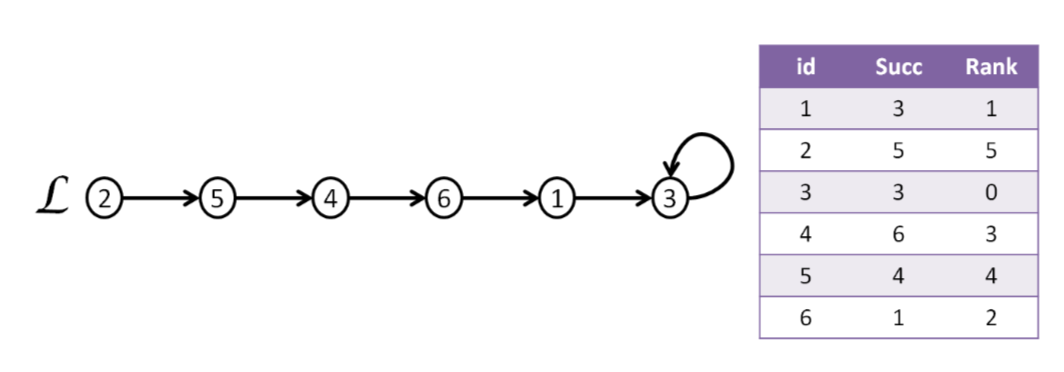
\includegraphics[width=\linewidth]{LinkedList.png}
 
\end{figure}

Ogni elemento della lista viene identificato con il suo id ovvero un intero che va da 1 a n. Per ogni elemento della lista manteniamo altre due informazioni, il rank e il successore.
L'ultimo elemento della lista ha come successore se stesso (viene creato un self-loop).
Ci sono tre metodi che possiamo utilizzare con il modello RAM per risolvere questo problema, questi metodi sfruttano l'accesso in memoria a costo costante:
\begin{itemize}
    \item Il primo metodo scorre la lista calcolando il numero (N) di elementi presenti al suo interno. Poi scorre di nuovo la lista e partendo dal primo elemento $i$ assegna il ranking $N-i$.
    \item Il secondo metodo crea un nuovo array di predecessori, in questo caso ogni elemento dell'array predecessori è nella forma $Pred[Succ(i)] = i$. Poi partendo dall'ultimo elemento assegno rank 0, poi 1, poi 2 ... poi assegno via via i vari rank.
    \item Un'ultima soluzione consiste nell'andare a calcolare il rank ricorsivamente. Il calcolo del rank viene svolto in questo modo: se $Succ[i] = i$ allora il $Rank(i)$ sarà pari a 0, altrimenti vado a calcolare ricorsivamente $Rank(i) = 1 + Rank(Succ(i))$
\end{itemize}

Questi metodi hanno una complessità che è O(n) ma il problema è legato al numero di operazioni I/O che vengono svolte perchè sono O(N) perchè l'accesso agli elementi non è continuo ma potrei saltare da una parte all'altra dell'array.
Quindi l'idea è quella di evitare di seguire i puntatori il più possibile per evitare alti costi per le operazioni di I/O.

\section{Tecnica del pointer Jumping}

La tecnica del pointer jumping consiste nell'utilizzo in parallelo di n processori che lavorano ognuno su un elemento della lista.
\begin{itemize}
    \item Ogni processore prende il suo elemento della lista e inizializza il rank a 0 se è l'ultimo elemento della lista mentre lo inizializza a 1 se è un elemento precedente.
    \item Ogni processore poi esegue le seguenti operazioni: prima calcola per il nodo i il rank corrispondente ovvero $Rank[i] += Rank[Succ[i]]$ poi calcola il successore del nodo i ovvero calcola $Succ[i] = Succ[Succ[i]]$.
\end{itemize}

Il valore del rank dei vari elementi della lista non cresce in modo lineare ma viene raddoppiato ad ogni step dell'algoritmo, questo vuol dire che la crescita è esponenziale e che il costo dell'esecuzione dell'algoritmo per ognuno degli n processori è $O(logn)$ in tempo. Complessivamente abbiamo un costo di $O(n*logn)$ operazioni svolte, perchè abbiamo n processori che svolgono $O(log n)$ operazioni.

\begin{figure}[h!]
  \centering
  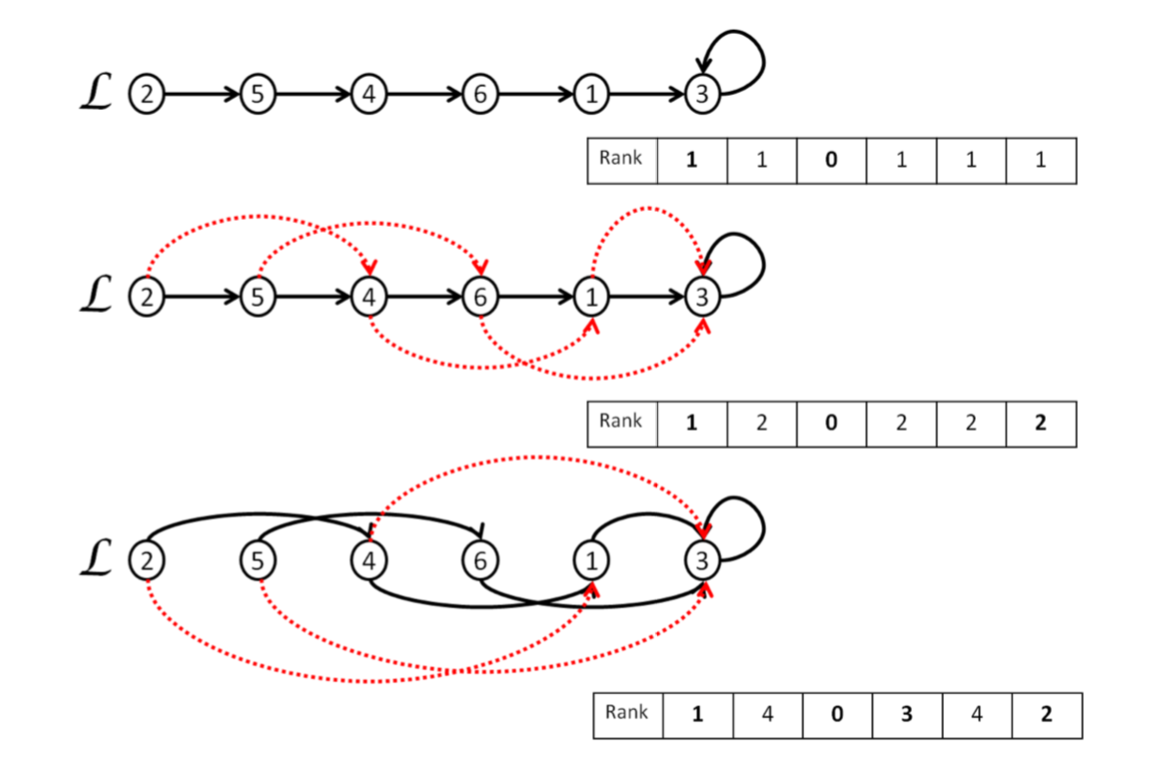
\includegraphics[width=\linewidth]{PointerJumping.png}
  
\end{figure}

\section{Simulazione dell'algoritmo con la memoria a 2 livelli}

Utilizzare la tecnica del Pointer Jumping nel modo in cui è stata descritta può comportare dei problemi per quel che riguarda il numero di operazioni I/O da effettuare perchè l'accesso in memoria può avvenire in modo totalmente random dato che gli elementi della lista non sono ordinati.
Per simulare il funzionamento delle due operazioni del pointer jumping (ovvero calcolo del successore e calcolo del rank) si usa il sorting e la scansione dell'array, il numero delle operazioni da effettuare è costante.
Le operazioni vengono simulate considerando la seguente forma $A[a_i]\ op\ A[b_i]$:
\begin{itemize}
    \item Nel caso dell'operazione di aggiornamento del rank l'"op" è la somma e l'assegnamento e A è l'array con i rank.
    \item Nel caso dell'operazione di ricerca del successore, op è l'operazione di assegnamento, A è l'array con i successori.
\end{itemize}

Questa operazione $A[a_i]\ op\ A[b_i]$ può essere eseguita in parallelo dagli n processori con un numero di operazioni di I/O pari a $O(\frac{n}{b})$, la simulazione consiste in 5 step:

\begin{itemize}
    \item Si crea per ogni elemento della lista una tripla in cui inseriamo $<a_i, b_i, 0>$ dove $a_i$ è l'id del nodo, $b_i$ è il successore e l'ultimo numero è il rank del nodo che, almeno all'inizio, viene settato a 0.
    \item Si fa un primo ordinamento delle triple basandoci sul secondo elemento.
    \item Si scorrono le triple e si creano delle nuove triple $<a_i, b_i, A[b_i]>$ dove $A[b_i]$ è il valore del rank del successore di $a_i$. (In questo caso l'operazione op è l'assegnamento perchè assegno il rank del successore).
    \item Si fa un secondo ordinamento basandoci sul primo elemento delle triple.
    \item Si fa la scansione delle triple e per ogni tripla si modifica il terzo valore andando a calcolare il nuovo rank (in questo caso è somma e assegnamento perchè sommiamo il rank che abbiamo con il rank del successore).
\end{itemize}

\textbf{Teorema: L'esecuzione in parallelo di n operazioni $A[a_i]\ op\ A[b_i]$ può essere simulata nella memoria a 2 livelli con un numero costante di scan e sort quindi abbiamo un numero di operazioni di I/O pari a $\frac{n}{B}$}
\newline \newline 
\textbf{Teorema: La simulazione dell'algoritmo del pointer jumping viene eseguita con la memoria a 2 livelli, sono necessari $O(log n)$ passaggi quindi il numero di operazioni di I/O da eseguire sono $\frac{n}{B}\ *\ logn $}.
\newline \newline 
\textbf{Teorema: Ogni algoritmo eseguito in parallelo su n processori che necessita di T step per terminare può essere simulato nella memoria a 2 livelli con un numero di operazioni di I/O pari a $\frac{n}{B}\ *\ T $}.
\newpage
Esempio di simulazione dell'algoritmo Pointer Jumping usando Scan e sort:

\begin{figure}[h!]
  \centering
  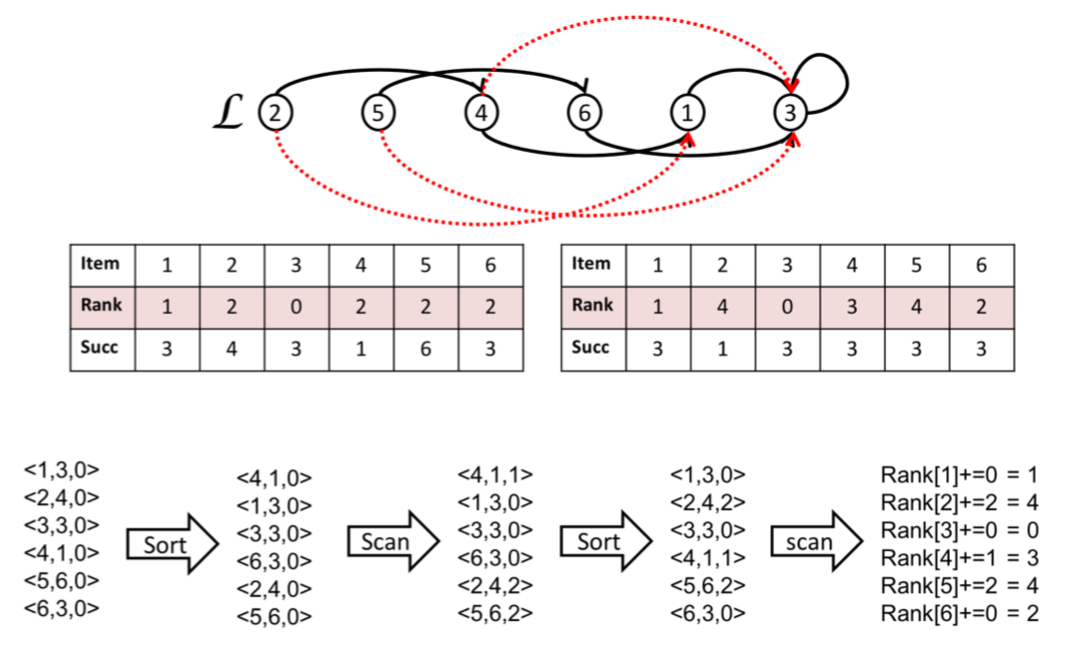
\includegraphics[width=\linewidth]{SimulazionePJ.png}
\end{figure}

\section{Approccio Divide & Conquer}



\fbox{\parbox{\dimexpr\linewidth-2\fboxsep-2\fboxrule\relax}{\begin{center}
    \textbf{Ripasso del Master Theorem}
    \end{center}
Il Master Theorem è il metodo che ci permette di risolvere le equazioni di ricorrenza del tipo: $T(N) = a\frac{n}{b} + f(n)$. Dove a indica il numero di sottoproblemi, $\frac{n}{b}$ indica la dimensione dei sottoproblemi e $f(n)$ indica il costo della divisione e della ricombinazione.
Nel Master Theorem abbiamo 3 casi differenti che vanno considerati per risolvere le equazioni di ricorrenza:
\begin{itemize}
    \item Calcoliamo $n^{log_b a - \epsilon}$, se $f(n)=O(n^{log_b a - \epsilon})$ ovvero $f(n)$ è minore allora la soluzione è $T(n) = \Theta(n^{log_b a })$.
    \item Calcoliamo $n^{log_b a - \epsilon}$, se $f(n)=\Theta(n^{log_b a - \epsilon})$ ovvero $f(n)$ è uguale allora la soluzione è $T(n) = \Theta(n^{log_b a }*log n)$.
    \item Calcoliamo $n^{log_b a - \epsilon}$, se $f(n)=\Omega(n^{log_b a - \epsilon})$ ovvero $f(n)$ è maggiore allora la soluzione è $T(n) = \Theta(f(n))$. Deve anche valere la condizione per cui $af(\frac{n}{b}) \leq c*f(n)$.
\end{itemize}
}
}
\newline\newline
Per risolvere il problema del List Ranking possiamo utilizzare un approccio ricorsivo che quindi consiste nel suddividere il problema nella fase di "Divide" andando poi a risolvere ricorsivamente il problema sul set di dati ridotto nella fase di "Conquer", alla fine nella fase di "Recombine" vengono ricombinate le soluzioni dei sottoproblemi.
Nel caso del problema del List Ranking le fasi sono le seguenti:

\begin{itemize}
    \item Divide: Creiamo un set I di elementi presi dalla lista iniziale, il set I deve essere tale che per ogni elemento presente in I, il successore dell'elemento non viene inserito nel set I. Questo vuol dire che la lunghezza del set I sarà $|I| \leq \frac{n}{2}$ e sarà $|I| > \frac{n}{c}$. Dove $c>2$.
    \item Conquer: Partendo dalla lista iniziale eliminiamo gli elementi che sono presenti in I e creiamo una seconda lista L'. Per ogni elemento x presente nella lista tale che $Succ[x]$ è presente in I dobbiamo andare a calcolare: $Rank[x] += Rank[Succ[x]]$ e poi $Succ[x] = Succ[Succ[x]]$. In questo modo il $Rank[x]$ indicherà per ogni x nella nuova lista la distanza tra x e il successore attuale di x.
    \item Recombine: in questa fase abbiamo calcolato il rank di tutti gli elementi presenti nella lista che abbiamo creato togliendo gli elementi del set I. Per ogni elemento x che appartiene a I dobbiamo andare a calcolare $Rank[x] = Rank[x] + Rank[Succ[x]]$ dove $ Rank[Succ[x]]$ indica la distanza tra il successore di x e la fine della lista ed è disponibile perchè l'abbiamo calcolato in precedenza dato che Succ[x] sta sicuramente nella lista L' che abbiamo creato.
    Mentre $Rank[x]$ indica la distanza tra x e il successore nella lista di partenza.
\end{itemize}

Un esempio:

\begin{figure}[h]
  \centering
  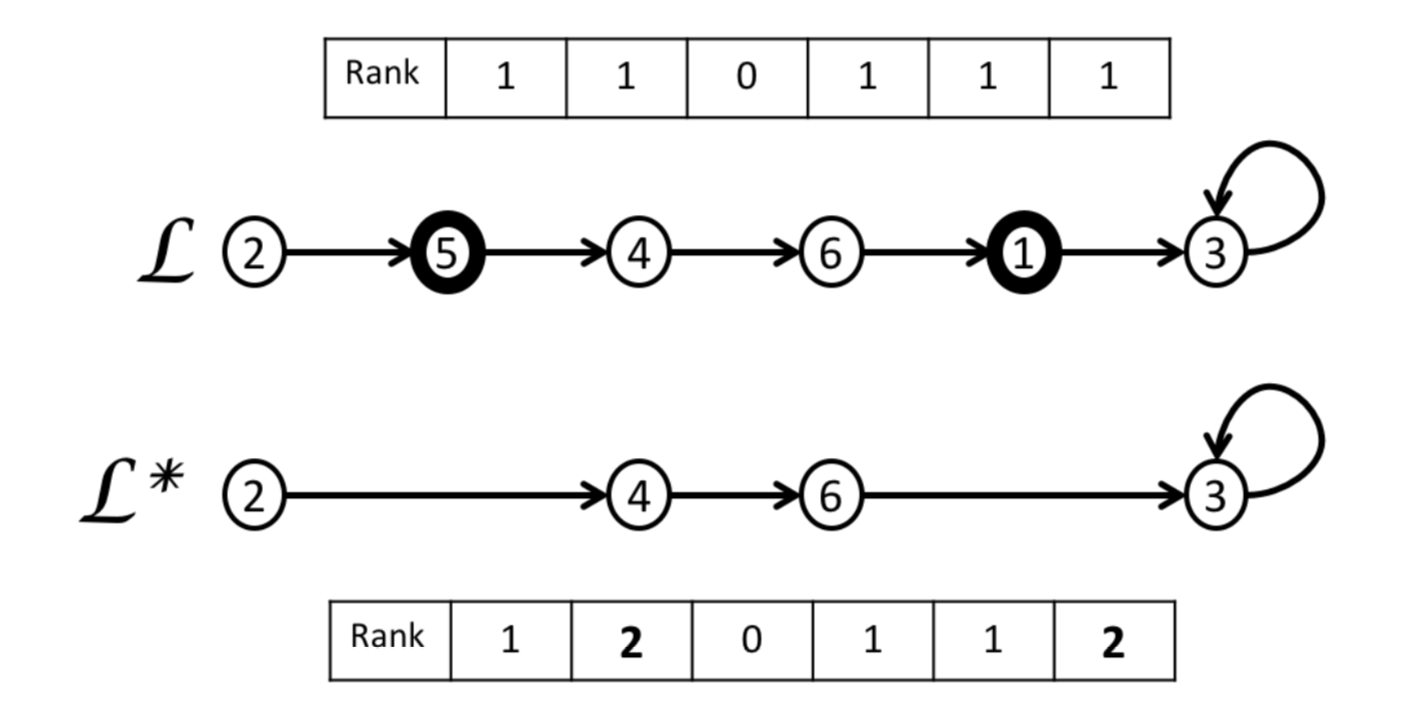
\includegraphics[width=0.8\linewidth]{ListRankingRec.png}
\end{figure}

Analizzando l'algoritmo, per capire il numero di operazioni I/O che vengono effettuate dobbiamo prendere in considerazione le tre fasi, divide, recombine e conquer.
In particolare per la fase di divide abbiamo un costo $I(n)$ che dipende dal modo in cui creiamo il set I. 
Per la fase di recombine abbiamo un costo che è $O(\frac{n}{b}$ e per la fase di conquer consideriamo il numero di elementi che rimangono nella lista L' ovvero $T((1-\frac{1}{c})n)$.
Quindi nel complesso abbiamo che il numero di operazioni di I/O viene indicato dalla seguente equazione di ricorrenza:
$T(n) = I(n) + O(\frac{n}{b} + T((1-\frac{1}{c})n)$.
Ora il problema sta nel modo in cui creiamo I perchè se scorriamo la lista e scegliamo se inserire o no l'elemento abbiamo un costo enorme in termini di I/O, quindi si deve trovare una alternativa.

\section{Coin Tossing}

\subsection{Coin Tossing randomizzato}

L'idea del coin tossing è che per ogni elemento della lista viene lanciata una monete, se esce testa e sull'elemento successivo esce croce allora vuol dire che posso selezionare l'elemento. Abbiamo 4 possibili configurazioni di testa e croce, quindi al più in I finiscono $\frac{n}{4}$ elementi.
Per il teorema che dice che l'esecuzione parallela su n processori può essere simulata con un numero costante di scan e sort con un numero di operazioni I/O pari a $\Theta(\frac{n}{b})$ allora possiamo dire che la I(n) di prima mi costa $\Theta(\frac{n}{b})$ al caso pessimo quindi possiamo riscrivere l'equazione di ricorrenza:
$T(n) = O(\frac{n}{b} + T(\frac{3n}{4})$.
Il $T(\frac{3n}{4})$ esce fuori perchè $I=\frac{1}{c}*n$ quindi L' diventa $|L'| = n - \frac{n}{c}$, se c=4 allora abbiamo che $|L'| = \frac{3}{4}$.
Risolvendo l'equazione (siamo nel caso 3) possiamo vedere che il list ranking utilizzando la procedura ricorsiva mi costa $O(\frac{n}{b})$.

\subsection{Coin Tossing Deterministico}

Con il coin tossing deterministico la procedura è differente e prevede vari step:

\begin{itemize}
    \item Per ogni elemento [1,n] della lista assegnamo un valore coin(i) pari a i-1. Quindi da 0 a n-1. Per rappresentare questo valore di coint(i) mi bastano $b = log n$ bit, per ogni elemento $bit_b$ indica questo valore del coin.
    \item Ora vogliamo passare da n valori del coin a 6 valori, per farlo:
        \begin{itemize}
            \item Per ogni i nella lista controlliamo $bit_b(i)$ e $bit_b(succ[i])$. Calcoliamo $\Pi(i)$ ovvero la posizione in cui i due valori differiscono e calcoliamo $z(i)$ ovvero il valore di $bit_b(i)$ che differisce rispetto a $bit_b(succ[i])$.
            \item Ora assegnamo $coin(i) = 2*\Pi(i) + z(i)$. Quindi ora mi bastano solamente $log(b) + 1$ bit per rappresentare il coin di i. 
        \end{itemize}
    \item Ora da 6 valori di coin vogliamo passare a 3 valori di coin. Per farlo consideriamo tutti gli elementi della lista che hanno un valore di coin compreso tra 3 e 5.
    Modifichiamo il loro valore di coin, $coin(i) = {1,2,3} - {Coin(pred(i)), Coin(succ(i))}$.
    \item Ora possiamo selezionare gli elementi di I, prendiamo tutti gli elementi tali che $coin(i) < coin(succ(i))$ e  $coin(i) < coin(pred(i))$.
\end{itemize}

Ci sono alcune cose da notare che fanno funzionare l'algoritmo:
\begin{itemize}
    \item È importante notare che non è possibile che i coin di due elementi vicini siano uguali, questo è fondamentale per l'ultimo passaggio ma anche per dimostrare la correttezza dello step in cui passiamo da 6 a 3 valori. Questa cosa non è possibile perchè se lo fosse avremmo $\Pi(i)+z(i) = \Pi(succ(i))+z(succ(i))$, quindi vorrebbe dire che $\Pi(i) = \Pi(succ(i))$ e questo implicherebbe l'assenza di differenze tra $bit_b(i)$ e $bit_b(succ(i))$. 
    \item Per quanto riguarda la complessità in termini di operazioni I/O, per passare da n valori di coin a 6 valori di coin, ogni volta ho una applicazione del logaritmo, quindi in pratica dobbiamo capire quante volte si effettua l'operazione del passaggio da n a 6 valori. Dato che la riduzione è logaritmica possiamo dire che vengono effettuate $log*n$ iterazioni. Vuol dire che applico * volte il logaritmo.
    Quindi ci metto poche iterazioni per passare da n a 6, quindi possiamo dire che per formare il set I abbiamo bisogno di $O(\frac{n}{b}*log*n)$, dato che $log*n$ cresce molto lentamente, possiamo considerarlo come una costante quindi abbiamo un numero di operazioni di I/O pari a $O(\frac{n}{b})$.
\end{itemize}

Quindi alla fine anche il coin tossing deterministico risolve il problema del list ranking con un numero di operazioni I/O che al caso pessimo saranno $O(\frac{n}{b})$.
Quindi questo è il caso migliore perchè abbiamo il caso pessimo e una situazione deterministica.

\chapter{Lezione 5: Ordinamento di array con elementi atomici}

In questo caso il problema è quello del sorting, abbiamo un array S con n elementi atomici e dobbiamo ordinarlo in modo crescente.
Con elementi atomici indichiamo quegli elementi che occupano un numero costante di celle di memoria.
C'è un altro problema che è legato al sorting, si tratta del problema del "permuting", in questo caso abbiamo un array S di n elementi e poi abbiamo un array $\Pi$ che mi indica la permutazione delle posizioni dell'array S di partenza. L'obiettivo è permutare gli elementi dell'array S andando a considerare l'ordinamento che viene indicato nell'array $\Pi$.
Nel modello Ram abbiamo che l'ordinamento costa in termini di tempo $O(nlogn)$ mentre la permutazione costa $O(n)$.
Se però pensiamo al modello con 1 disco e una memoria interna dobbiamo pensare al costo in termini di operazioni I/O che dobbiamo effettuare. In questo caso il vero problema è legato non al sorting dei dati quanto invece all'accesso ai dati, abbiamo quindi un I/O Bottleneck. Permutare gli elementi di un array con un modello con 1 disco mi comporta un numero di accessi al disco (Operazioni I/O) che è $O(n)$ e soprattutto che non è per niente efficiente perchè carico un blocco e poi accedo magari solamente ad un elemento del blocco sfruttando quindi solamente $\frac{1}{B}$ del blocco.

\section{Il Merge Sort}

Vogliamo considerare l'esecuzione dell'algoritmo Merge Sort nel modello con una memoria esterna da cui leggiamo blocchi di dati di dimensione B e una memoria interna di dimensione M.
Il Merge sort è un algoritmo Divide et Impera, il codice:

\begin{code}
\begin{lstlisting}[escapeinside={(*}{*)}]
MergeSort(S,i,j):
    if(i<j):
        m = (i+j)/2
        MergeSort(S,i,m-1)
        MergeSort(S,m,j)
        Merge(S,i,m,j)
\end{lstlisting}
\end{code}

Nel codice abbiamo un primo controllo iniziale, con l'if controlliamo di avere un array di dimensione maggiore di 1 elemento. Poi abbiamo le due chiamate ricorsive a MergeSort che contribuiscono a suddividere il problema in due sottoproblemi generando due array. Il numero complessivo delle chiamate ricorsive che vengono effettuate è $O(log n)$ perchè ogni volta la dimensione dell'array da ordinare viene divisa in 2.
La chiamata Merge invece serve per unire i due sotto array, per svolgere questa unione utilizziamo due puntatori che utilizziamo per confrontare i due elementi dell'array, il costo della procedura Merge è $O(n)$. Quindi nel complesso il costo è $O(nLogn)$.
Alla fine l'array ordinato non è quello iniziale ma ne abbiamo uno nuovo, quindi la complessità in spazio è $O(n)$ e l'ordinamento non viene eseguito in-place.

La situazione si fa più complicata quando l'array da ordinare non entra completamente nellla memoria interna di dimensione M ovvero quando $n>M$.
In questo caso va considerato più di tutti il costo necessario per svolgere le operazioni di I/O.
Per calcolare il numero delle operazioni I/O che dobbiamo eseguire vanno considerati i seguenti aspetti:
\begin{itemize}
    \item Ammesso di avere una memoria interna M che ci permette di mantenere almeno due pagine di dimensione B ($M \geq 2B$), consideriamo il Merge, abbiamo due sotto array di dimensione x e dobbiamo andare a unire questi sotto array ordinati in un unico array.
    Il numero di operazioni di I/O in lettura per eseguire il merge sono $O(x/B)$ per il primo sotto array e altrettanti per il secondo. Quindi nel complesso abbiamo $O(x/B)$ operazioni di I/O.
    Per la scrittura il discorso è simile, devo scrivere nell'array destinazione x elementi che sono posizionati in modo contiguo quindi avremo sempre un numero di operazioni I/O pari a $O(x/B)$.
    Quindi complessivamente la complessità del Merge Sort la possiamo indicare con la seguente equazione di ricorrenza: $T(N) = 2T(\frac{n}{2}) + O(\frac{n}{b})$ quindi il costo del Merge Sort è $O(\frac{n}{B}Logn)$.
    \item Nella prima parte del ragionamento non abbiamo considerato una cosa importante, ad un certo punto dividendo l'array arriveremo ad un sotto array di dimensione $z = O(m)$ che quindi mi costa $O(z/B)$ operazioni di I/O per essere caricato in memoria ma poi non mi costa ulteriormente perchè è tutto in memoria e non devo fare altre operazioni di I/O.
    Questa idea la posso applicare su un numero di sotto array pari a $O(n/M)$. 
    Questo comporta che al costo di $O(\frac{n}{B}Logn)$ che avevo in precedenza per le operazioni di I/O (che era derivato dal fatto che ho Logn passaggi di divisione) devo andare a togliere il numero di step che verrebbero fatti dal momento in cui i dati entrano totalmente in memoria ovvero $O(\frac{n}{B}LogM)$.
    Quindi complessivamente abbiamo $O(\frac{n}{B}Logn) - O(\frac{n}{B}LogM)$ ovvero un numero di operazioni I/O pari a $O(\frac{n}{B}Log\frac{n}{M})$.
\end{itemize}

\subsection{Come migliorare il Merge Sort}

Abbiamo detto che il numero di operazioni di I/O che svolge il Merge Sort se l'array da ordinare non entra tutto in memoria è $O(\frac{n}{B}Log\frac{n}{M})$.
Sarebbe più corretto scrivere che il numero di operazioni di I/O è $O(\frac{n}{B}Log\frac{n}{cM})$ dove la c è uguale a 1 nel caso dell'heap sort perchè l'ordinamento viene effettuato in place, è poco meno di 1 nel caso del quick sort per via delle chiamate ricorsive mentre è 0.5 nel caso del Merge Sort perchè devo anche mantenere un array in cui inseriamo i valori ordinati.
Quindi per diminuire il numero di operazioni da effettuare o aumentiamo la dimensione di B, o aumentiamo la dimensione di M oppure cambiamo il valore del 2 del logaritmo.
Ci sarebbe anche la possibilità di andare ad comprimere i run ordinati utilizzando il gap encoding e poi qualche algoritmo di compressione di interi, in questo modo in memoria entrano più elementi di S.

Ci sono due possibili soluzioni che possono essere adottate.

\subsubsection{Snow Plow}

È un metodo che è stato proposto da Knuth, noi sappiamo che nel merge sort creiamo n/M blocchi ordinati e per ordinarli non abbiamo costi di I/O perchè sono grandi M ed entrano in memoria interna.
L'idea è quella di aumentare virtualmente M andando a creare dei run ordinati di dimensione 2M. In questo modo riduciamo la profondità a cui si arriva (e che comporta operazioni di I/O) che quindi non sarà più $log(\frac{n}{M})$ ma $log(\frac{n}{2M})$.
La tecnica Snow Plow permette di aumentare virtualmente la memoria interna di un fattore 2 (in media) quindi alla fine avremo un numero di operazioni di I/O pari a $O(\frac{n}{B}(log(\frac{n}{2M}))s$.

L'algoritmo utilizza:
\begin{itemize}
    \item Tutta la memoria interna di dimensione M
    \item All'interno della memoria M viene creato un Min-Heap H (che non consuma spazio)
    \item Viene utilizzato un array U.
\end{itemize}

L'algoritmo funziona in questo modo:

\begin{itemize}
    \item Nella prima fase andiamo a prendere M elementi dall'array S da ordinare e li inseriamo nel Min Heap H.
    \item Ora entriamo in un while, fino a quando il Min-Heap non è vuoto, estraiamo il minimo da H e lo scriviamo nel run in output, poi prendiamo un elemento da S, se è maggiore del minimo estratto lo mettiamo nello heap, altrimenti nell'array U.
    \item Quando si svuota il Min-heap vuol dire che invece U sarà pieno, ci saranno M elementi, a questo punto ricominciamo dal punto precedente andando a inserire gli elementi di U nello heap e rientriamo poi nel while.
\end{itemize}

Il codice completo è il seguente:

\begin{code}
\begin{lstlisting}[escapeinside={(*}{*)}]
H = Creare un Min Heap partendo dall$'$array U
U = vuoto
while(H non vuoto):
    Min = Estrai il minimo da H
    Scrivi min sul run in output
    prendi un elemento x da S
    if(x < min):
        Add x to U
    else:
        Add x to H
\end{lstlisting}
\end{code}

Ora bisogna considerare quanto scrivo in output e quanto leggo da S prima che si svuoti il Min Heap.
\begin{itemize}
    \item Diciamo che leggiamo da S un numero di elementi pari a $\tau$, quindi vuol dire che di questi elementi almeno M devono andare a finire in U
    \item Quindi in H ci finiscono $\tau - M$ elementi
    \item Vuol dire che in output, per ogni run ci finiscono M elementi che stavano già nello heap più $\tau - M$ elementi che ho inserito. Ovvero ci finiscono $\tau$ elementi.
    \item Se consideriamo che gli elementi di S hanno una probabilità uniforma di essere minori del minimo dello heap o di essere maggiori, allora possiamo dire che $\frac{\tau}{2}$ elementi letti da S finiscono in H e $\frac{\tau}{2}$ finiscono in U.
    \item Dato che sappiamoc che in U ci devono finire M elementi possiamo dire che $\frac{\tau}{2} = M$ Ovvero  $\tau = 2*M$.
    Quindi leggiamo $\tau = 2*M$ elementi da S.
\end{itemize}

Cosiderando tutto questo possiamo dire che utilizzando Snow Plow, verranno creati un numero di run ordinati pari a $O(\frac{n}{M}$ ma ognuno di questi run sarà più lungo di M, in media sarà $2M$. Quindi in pratica ora non devo arrivare fino ai run lunghi M per non avere più operazioni di I/O ma mi basterà arrivare ai run grandi 2M.
Quindi la complessità in termini di I/O del Merge sort utilizzando Snow Plow diventa in media $O\frac{n}{b}log(\frac{n}{2M})$.

\section{Multi Way Merge Sort}

Con Snow Plow siamo passati ad una complessità delle operazioni di I/O del Merge Sort che è (nel caso del 2 disk level) in media $O\frac{n}{b}log(\frac{n}{2M})$. Ovvero abbiamo raddoppiato "virtualmente" la dimensione di M.

Nel MultiWay Merge Sort invece si lavora sulla base 2 del logaritmo.
Quando facciamo il merge dei vari run, con il classico Merge Sort andiamo a prendere due run alla volta e facciamo il merge, vuol dire che in memoria ci troviamo solamente due blocchi per leggere e uno per scrivere mentre tutto il resto rimane inutilizzato.
In pratica in memoria potremmo tenere un numero di blocchi per leggere $k = M/B\ -\ 1$ e invece ne teniamo solamente 2.
L'idea quindi è quella di andare ad aumentare il numero dei blocchi che sono presenti in memoria e da cui vogliamo prendere elementi da mergiare. In particolare dato che vogliamo inserire k blocchi, vorremo confrontare k elementi (1 per ogni blocco) e restituirli in output.

L'idea è di utilizzare un Min Heap, carichiamo k blocchi in memoria interna e poi leggiamo il primo elemento dei k blocchi e lo inseriamo all'interno del Min Heap.
Per ogni elemento del Min Heap non ci salviamo solamente il suo valore ma anche il run da cui proviene, in questo modo quando estraiamo il minimo dal Min Heap per metterlo in output, potremo andare nel run corrispondente per estrarre un altro elemento da quello specifico run. Il processo di merging richiede un tempo $O(log k)$ per ogni singolo elemento e poi, presi k run la cui lunghezza è pari a z richiede un numero di operazioni di I/O pari a $O(z/B)$.
In questo modo riusciamo ad aumentare il 2 della base del logaritmo che diventa $M/B$ perchè ora non uniamo più due run alla volta ma $k = M/B -1 $.
Quindi complessivamente il Multi Way Merge Sort richiede una compelessità in termini di tempo pari a $O(nlogn)$, il numero di operazioni di I/O però scende a $O(\frac{n}{b}log_{\frac{M}{B}}\frac{n}{M})$.


\section{Lower Bound}

Consideriamo due problemi, il sorting e il permuting. 
Nel Ram model possiamo dire che il lower bound del sorting è $\Omega(nLogn)$ mentre il permuting è $O(n)$ perchè faccio degli spostamenti accedendo in memoria e gli accessi però non li pago.
Ora consideriamo il 2 disk model, in questo caso il numero di operazioni I/O che pago per il sorting è identico al numero di operazioni I/O che pago per il permuting, questo vuol dire che abbiamo un collo di bottiglia per quel che riguarda lo spostamento dei dati nel disco e non nel sorting.

Per la soluzione del problema del permuting abbiamo due metodi nel caso del 2-disk model:
\begin{itemize}
    \item Simuliamo quello che succede nel modello ram ovvero abbiamo la lista S, la lista delle permutazioni $\Pi$ e poi creiamo la lista S' andando a mettere in ogni posizione i di S' l'elemento $S[\Pi[i]]$.
    Questo mi costa $O(n)$ operazioni di I/O.
    \item Possiamo usare il sorting per risolvere il problema del permuting. Si fa così:
        \begin{itemize}
            \item Creiamo una sequenza di coppie $<i, \Pi[i]>$ dove i è la posizione in cui $S[\Pi[i]]$ deve essere posizionato
            \item Si fa un primo sort sul secondo elemento della coppia.
            \item Si fa una operazione di Scan sostituendo $\Pi[i]$ con $[\Pi[i]]$
            \item Si fa un sort sul primo elemento delle coppie
        \end{itemize}
    L'algoritmo fa due ordinamenti e una scansione, tutto questo mi costa un numero di I/O pari a $O(\frac{n}{B}log_{\frac{M}{B}\frac{n}{m}})$.
    
\end{itemize}
Quindi in generale l'operazione di permuting nel 2 level model mi costa un numero di I/O pari a $min(n,\frac{n}{B}log_{\frac{M}{B}\frac{n}{m}})$.


\subsection{Lower Bound per il sorting con modello RAM}

Per calcolare il lower bound del sorting nel modello Ram dobbiamo utilizzare un albero di decisione, in ogni nodo dell'albero viene presa una decisione e ogni nodo poi ha due figli. Quindi l'albero è binario e se abbiamo n elementi da ordinare avremo $n!$ possibili ordinamenti che quindi corrispondono a $n!$ foglie dell'albero.
Ogni path dal nodo root ad una foglia è una possibile computazione.
Se l'albero ha altezza h vuol dire che all'ultimo livello dell'albero dovremo avere $n!$ foglie, quindi:
\begin{equation}
    2^h \geq n! => h \geq log n! => h \geq n log n
\end{equation}
L'ultimo passaggio lo possiamo fare per l'approssimazione di Stirling. Quindi il lower bound nel ram model è $\Omega(nlogn)$

\subsection{Lower Bound per il sorting con 2 Level Model}

Anche in questo caso dobbiamo sempre considerare l'albero di decisione in cui ogni nodo è un confronto e una operazione di I/O. Il numero delle foglie è sempre $n!$. 
La differenza rispetto al modello ram è il numero di figli di ogni nodo (fan-out), un solo I/O legge B elementi e ce ne sono già M-B in memoria, questo I/O mi genera un numero di possibili ordinamenti differenti dei B elementi che è pari a $\binom{M}{B}$ modi differenti, vanno però considerate anche le possibili permutazioni di B che sono $B!$ quindi il fan out dei nodi è $(\binom{M}{B})B!$.
Va considerato anche un altro dettaglio però, dopo aver fatto O(n/b) I/O avremo già considerato tutti gli elementi una volta, quindi non è necessario considerare le possibili permutazioni di B quindi per alcuni livelli dell'albero di decisione il fan out dei nodi sarà $(\binom{M}{B})$.

Se consideriamo un percorso root-foglia lungo t avremo $\frac{n}{b}$ nodi che avranno un fan out $(\binom{M}{B})B!$ e $t-b$ nodi che invece avranno un fan out $(\binom{M}{B})$.
Quindi il numero delle foglie dell'albero sarà:
\begin{equation}
    ((\binom{M}{B})B!)^{\frac{n}{B}} * (\binom{M}{B})^{t-\frac{n}{B}} 
\end{equation}

Questo va posto sempre maggiore o uguale a $n!$ perchè il numero di foglie deve essere quello quindi abbiamo:

\begin{equation}
    ((\binom{M}{B})B!)^{\frac{n}{B}} * (\binom{M}{B})^{t-\frac{n}{B}} \geq n! = (\binom{M}{B})^{t}*(B!)^{\frac{n}{B}}\geq n!
\end{equation}
\begin{equation}
    t Log(\binom{M}{B}) * \frac{n}{B}Log(B!) \geq Log n!
\end{equation}
\begin{equation}
    t Log(\binom{M}{B}) * B\frac{n}{B}Log(B) \geq nLog n
\end{equation}
\begin{equation}
    t Log(\binom{M}{B}) * n Log(B) \geq n Log n
\end{equation}
\begin{equation}
    t Log(\binom{M}{B}) \geq n Log n - n Log(B)
\end{equation}
\begin{equation}
    t Log(\binom{M}{B}) \geq n Log \frac{n}{B}
\end{equation}

Con la formula del cambio di base:

\begin{equation}
    t \geq \frac{n}{B} Log_{\frac{M}{B}} \frac{n}{B}
\end{equation}

Quindi vuol dire che il numero di operazioni I/O da eseguire è pari a $\frac{n}{B} Log_{\frac{M}{B}} \frac{n}{B}$.
Se abbiamo invece D dischi diventa $\frac{n}{DB} Log_{\frac{M}{B}} \frac{n}{DB}$.


\subsection{Lower bound per le permutazioni (SENZA DIMOSTRAZIONE)}

Nel caso delle permutazioni il lower bound è $\Omega(n)$ se $B*log(\frac{M}{B})\leq logn$.
Altrimenti è $\Omega(\frac{n}{B}Log_{\frac{M}{B}}\frac{n}{M})$

\section{Distribution Based sorting paradigm}

Il Quick Sort è un altro algoritmo di ordinamento che è sempre ricorsivo come il Merge Sort ma non ha lo step di recombine perchè l'ordinamento viene effettuato in-place e soprattutto l'efficienza dell'algoritmo dipende dal modo in cui viene suddiviso l'array su cui vengono poi effettuate le chiamate ricorsive.
Il codice di QuickSort:
\begin{code}
\begin{lstlisting}[escapeinside={(*}{*)}]
QuickSort(S,i,j):
    if(i<j):
        r = posizione del pivot che scelgo
        inverti S[r] con s[i]
        p = partition(S,i,j)
        QuickSort(S,i,p-1)
        QuickSort(S,p+1,j
\end{lstlisting}
\end{code}

La chiave del Quick Sort è l'utilizzo di un pivot e della procedura partition che divide l'array in due parti, una parte contiene gli elementi dell'array minori del pivot e una parte gli elementi dell'array maggiori del pivot.
La scelta del pivot è importante perchè più riusciamo a creare due sub array bilanciati su cui fare la ricorsione e più abbiamo la possibilità di raggiungere una complessità in termini di tempo pari a $O(nLogn)$ così come avviene nel Merge Sort, nel caso pessimo (un sub array enorme e uno vuoto) abbiamo invece una complessità pari a $O(n^2)$.
Per migliorare il QuickSort proviamo a modificare il modo in cui si effettua il partizionamento dell'array.

\subsection{3 Way Quick Sort}

Il classico algoritmo Partition ci permette di suddividere l'array di partenza in due sub array, uno con gli elementi minori del pivot e uno con i maggiori. Questo algoritmo modifica l'array originale che quindi viene riordinato seguendo questa regola. Il costo di una singola esecuzione di partition è $O(n)$.
Possiamo modificare Partition per fare in modo che una parte dei dati presenti all'interno dell'array non venga considerata nelle successive chiamate ricorsive.
Invece che dividere l'array in due parti si passa ad una divisione in 3 parti, in particolare avremo la sezione dell'array con gli elementi di valore minore del pivot, gli elementi uguali al pivot e poi i maggiori del pivot.
Questo mi permette di non considerare nelle successive iterazioni tutti gli elementi uguali al pivot.
Il codice dell'algoritmo è il seguente:
\begin{code}
\begin{lstlisting}[escapeinside={(*}{*)}]
Partition(S,i,j):
    P = S[i], l = i, r = i+1
    for(c=r;c $\leq$ j; c++):
        if(S[c] == P):
            inverti S[c] con S[r]
            r++
        else if(S[c] < P):
            inverti S[c] con S[l]
            inverti S[c] con S[r]
            r++
            l++
    return l,r-1
\end{lstlisting}
\end{code}

Questa modifica di partition deve restituire due valori, uno è l che indica il punto in cui finisce la zona minori e uno è r-1 che indica il punto in cui inizia la zona maggiori, questo mi permette di evitare di effettuare le prossime chiamate ricorsive sugli elementi di valore uguale al pivot.
Nell'algoritmo fissiamo P che diventa il pivot ed è il primo elemento dell'array, poi abbiamo l e r che sono i delimitatori delle varie zone del sub array, quando trovo un elemento uguale al pivot aumento la zona dell'uguale andando ad aumentare il valore di r, se invece ne trovo uno minore devo aumentarli entrambi perchè sposto quello che trovo al posto del primo uguale e il primo uguale va al posto di quello minore che ho trovato. Se trovo un valore maggiore del pivot invece non faccio niente perchè sta già al suo posto.
Quindi l'array S[1,c-1] che voglio analizzare sarà divisibile in 3 parti:
\begin{itemize}
    \item S[1,l-1] = elementi di valore minore del pivot
    \item S[l,r-1] = elementi di valore uguale al pivot
    \item S[r,c-1] = elementi di valore maggiore del pivot
\end{itemize}

\subsection{Selezione del Pivot}

La scelta del pivot da utilizzare è fondamentale, se scelgo bene il pivot allora riduco anche il numero di confronti che faccio e la dimensione dei sub array su cui richiamo ricorsivamente Quick Sort.
Una buona strategia consiste nella scelta random del valore del pivot, questo rende QuickSort non prevedibile, però possiamo dire che in media la complessità in tempo è sempre $O(nLogn)$ mentre il numero di confronti che vengono effettuati sono, in media non più di $2nlogn$.

Dimostrazione che il numero di confronti non supera $2nlogn$:

\begin{itemize}
    \item Consideriamo $X_{u,v}$ che è la variabile che mi indica se S[u] e S[v] sono state confrontate o no e poi $p_{u,v}$ che invece mi dice la probabilità di confrontare questi due valori.
    \item La media dei confronti quindi dipende dalla probabilità $p_{u,v}$ che quindi va stimata.
    \item Per stimare $p_{u,v}$ consideriamo vari casi:
        \begin{itemize}
            \item Se abbiamo scelto un pivot S[r] tale che S[u] e S[v] sono sempre maggiori o sempre minori allora vuol dire che non facciamo mai confronti tra S[u] e S[v].
            \item Se invece scegliamo come pivot S[u] oppure S[v] allora facciamo almeno un confronto tra i due, gli altri casi sono quando il pivot è compreso tra u e v.
            Per il calcolo della $p_{u,v}$ ordiniamo S e otteniamo S', poi prendiamo il corrispondente di S[u] e di S[v] in S'che stanno in posizione u' e v' e calcoliamo $v'-u'+1$.
            La $p_{u,v}$ quindi è 2 sulla distanza tra u' e v' quindi: $p_{u,v} = \frac{2}{v'-u'+1}$ 
        \end{itemize}
\end{itemize}
Ora data questa probabilità possiamo dimostrare che non facciamo più di $2nLogn$ confronti:

\begin{equation}
    E[\sum_{u,v}X_{u,v}] = \sum_{u'=1}^{n} \sum_{v'>u'}^{n} \frac{2}{v'-u'+1} = 2 \sum_{u'=1}^{n} \sum_{k=2}^{n-u'+1} \frac{1}{k} \leq 2nLogn
\end{equation}

L'ultimo passaggio è giustificato dalla proprietà della serie armonica.


Per rendere ancora più random la scelta possiamo usare un'altra strategia, non prendiamo un solo pivot ma ne prendiamo più di uno, ad esempio 3 e poi consideriamo il valore medio tra questi tre e lo usiamo come pivot, in questo caso il costo dei confronti è O(1) a cui va sommato il costo O(n) di partition. Se aumentiamo il numero di valori da considerare per poi calcolare la media andiamo ad aumentare il costo di partition fino a $O(nLogN)+O(n)$.
Possiamo ridurre questo costo a O(N) con un algoritmo che è RandSelect ed è simile all'algoritmo Partition, solo che serve solamente a selezionare il pivot, il codice dell'algoritmo è il seguente:

\begin{code}
\begin{lstlisting}[escapeinside={(*}{*)}]
RandSelectt(S,k):
    r = elemento random da S
    $S_<$ = elementi di S più piccoli di S[r] 
    $S_>$ = elementi di S più grandi di S[r]
    $n_<$ = |$S_<$|
    $n_=$ = |S| - ($S_<$ + $S_>$)
    if(k $\leq$ $n_<$):
        return RandSelect($S_<$, k)
    else if((k $\leq$ $n_<$ + $n_=$):
        return S[r]
    else
        return RandSelect($S_>$, k- $n_<$ -  $n_=$)
\end{lstlisting}
\end{code}

Qui S[r] funziona come il pivot di quicksort e consideriamo k che è il rank dell'elemento che vogliamo usare come pivot.
L'array è comunque diviso in tre parti ma a differenza di QuickSort andiamo ricorsivamente solamente su una di queste tre parti ovvero quella che contiene l'elemento di rank k, se capitiamo subito nel caso in cui il rank è uguale a S[r] allora restituiamo subito S[r].
Il costo di questo algoritmo in termini di tempo è $O(n)$ nel Ram model e richiede $O(\frac{n}{B})$ operazioni di I/O nel 2 level model.
Dimostrazione:
    \begin{itemize}
        \item Consideriamo una buona scelta del Pivot quella che fa in modo che le partizioni $n_<$ e $n_>$ non siano più grandi di $\frac{2n}{3}$. Per fare in modo che valga questa proprietà allora l'elemento che cerchiamo deve avere un rank compreso tra [$\frac{n}{3}$, $\frac{2n}{3}$].
        \item La probabilità di essere in questo range è $\frac{1}{3}$ perchè equivale alla probabilità di essere nel sub array di mezzo.
        \item Quindi bisogna scrivere l'equazione di ricorrenza considerando la buona scelta dle pivot e la cattiva:
        \begin{equation}
            T(n) \leq O(n) + \frac{1}{3}T(\frac{2n}{3}) + \frac{2}{3}T(n)
        \end{equation}
        Dove il primo elemento è dovuto alla complessità dello spostamento degli elementi nell'array, il secondo è il costo del caso con la scelta buona del pivot (perchè ho 1/3 di probabilità che $n_<$ e $n_>$ non siano più grandi di $\frac{2n}{3}$) e poi l'ultimo è il caso in cui invece si fa la ricorsione su praticamente tutto l'array.
        Questa equazione si risolve sottraendo T(n) da entrambe le parti:
        \begin{equation}
            T(n) \leq O(n) + \frac{1}{3}T(\frac{2n}{3})
        \end{equation}
        Questo equivale a O(n) nel caso del Ram model, nel caso del 2 level l'equazione diventa:
        \begin{equation}
            T(n) \leq O(\frac{n}{b}) + \frac{1}{3}T(\frac{2n}{3})
        \end{equation}
        E quindi il numero di I/O diventa $O(\frac{n}{b})$.
    \end{itemize}
    
\section{Bounded Quick Sort}

Il QuickSort è un algoritmo che effettua l'ordinamento in-place quindi non è necessario dello spazio extra come invece accade in Merge Sort.
In realtà anche con il Quick Sort abbiamo bisogno di spazio extra perchè quando eseguiamo le chiamate ricorsive dobbiamo salvare il valore delle variabili del chiamante, per ogni chiamata abbiamo bisono di $\Theta(1)$ spazio. Dato che facciamo $\Omega(n)$ chiamate ricorsive avremo una complessità in termini di spazio pari a $\Theta(n)$.

Dobbiamo ridurre questa complessità e possiamo farlo con il Bounded QuickSort, il codice è il seguente:

\begin{code}
\begin{lstlisting}[escapeinside={(*}{*)}]
BoundedQS(S,i,j):
    while(j-i > $n_0$):
        r = pick a random pivot
        p = Partition(S, i, j)
        if(p $\leq$ $\frac{i+j}{2}$):
            BoundedQS(S,i,p-1)
            i = p+1
        else:
            BoundedQS(S, p+1, j)
            j = p - 1
    InsertionSort(S,i,j)
\end{lstlisting}
\end{code}

In questo caso si utilizzano sia le chiamate ricorsive sia il while sia l'insertion sort.
In particolare viene fatto subito un confronto tra j-i e un valore $n_0$ che viene scelto da noi e non deve essere troppo alto. Se non entriamo nel while viene eseguito l'algoritmo insertion sort che, in caso di array non troppo grandi è efficiente.
Quando entriamo nel while eseguiamo la chiamata ricorsiva del BoundedQS sulla parte più breve del sub array, quella dove troviamo il pivot. Poi andiamo avanti sulla parte pià lunga del sub array con il while ed eseguiamo la chiamata ricorsiva solamente su metà di questo sub array. Questa tecnica che riduce la dimensione del sub array su cui facciamo la ricorsione si chiama "elimination of the tail recursion" e ci permette di eseguire solamente $O(log_2 n)$ chiamate ricorsive sprecando quindi solamente $O(log_2 n)$ spazio aggiuntivo.

\section{MultiWay QuickSort}

Così come avviene con il Merge Sort, in cui andiamo a migliorare l'efficienza in termini di scritture e letture dal disco andando a mergiare k run in contemporanea, anche con il Quick Sort vogliamo massimizzare l'efficienza da questo punto di vista.
L'idea in questo caso è quella di utilizzare k-1 pivot e dividere in questo modo l'array che vogliamo partizionare in k sub array.
La k che vogliamo usare per dividere l'array deve essere tale che $k=O(\frac{M}{B})$ ovvero vogliamo che il numero di sub array che creo sia pari al numero di blocchi che possono essere contenuti in memoria, ognuno di questi blocchi però dovrà avere una quantità di elementi pari a $O(\frac{n}{k})$ per fare in modo che la suddivisione sia bilanciata.

Nella memoria quindi andremo ad avere 1 blocco in cui mettere i dati in input e k-1 blocchi di output che utilizziamo per scrivere le partizioni mentre le formiamo. Ogni fase del partition mi costa un numero di operazioni I/O pari a $\frac{n}{B}$ (per precisione sarebbero $\frac{n}{B}$ per scrivere e $\frac{n}{B}$ per leggere).
Sapendo che abbiamo k blocchi in memoria, possiamo capire il numero di volte che verrà eseguita la fase partition ovvero $O(\frac{n}{B}Log_{\frac{M}{B}}(\frac{n}{M}))$.

Per riuscire ad avere questo costo in termini di operazioni di I/O è necessario che i k-1 pivot siano scelti in modo corretto e per questo si utilizza un algoritmo che sfrutta l'oversampling, il codice è il seguente:

\begin{code}
\begin{lstlisting}[escapeinside={(*}{*)}]
Crea (a-1)(k-1) sample di dati dalla sequenza in input
Ordinali in A
For i=0 to len(A):
    prendi come pivot l'elemento A[(a+1)i]
return the pivots
\end{lstlisting}
\end{code}

L'idea è quella di selezionare non solo k-1 pivot ma un numero superiore di pivot.
Selezionando questo maggior numero di pivot andiamo ad ottenere dei pivot finali più distribuiti lungo la sequenza dei dati perchè selezioniamo il primo poi saltiamo di a+1 e selezioniamo il secondo e così via.
In particolare se scegliamo una a molto alta (vicino a n/k) avremo una distribuzione quasi perfetta dei dati perchè ogni sequenza sarà formata più o meno da n/k dati, allo stesso tempo aumenterà il tempo per il sorting e potremmo non riuscire a mettere in memoria tutti i dati da ordinare.
Al contrario con una a troppo vicina a 0 avremmo un ordinamento veloce ma dei sub array poco bilanciati.
Un buon risultato lo otteniamo se scegliamo $a=\Theta(Log k)$ e in questo modo ogni subset non presenta più di $O(\frac{n}{k}$ elementi.

\subsubsection{Lemma}

Lemma: Dati $k \geq 2$ e a+1 = 12*ln k, un sample di dimensione $(a+1)k-1$ mi basta per dire che ogni bucket riceve meno di $\frac{4n}{k}$ elementi con probabilità almeno $\frac{1}{2}$.

Dimostrazione: Consideriamo il problema complementare e lavoriamo tramite failure sampling, diciamo che esiste 1 bucket che contiene più di $\frac{4n}{k}$ elementi con probabilità al più $\frac{1}{2}$.
Prendiamo la versione ordinata di S, la chiamiamo S' è formata da $\frac{k}{2}$ blocchi di dimensione $\frac{2n}{k}$ elementi.
Ora consideriamo:
\begin{itemize}
    \item Un blocco $B_i$ tale che la dimensione sia almeno $\frac{4n}{k}$, questo blocco si sovrappone ad un blocco $t_i$ della sequenza e i suoi delimitatori saranno esterni a $t_i$ e saranno ad esempio $s_i$ e $s_{i-1}$.
    \item Ora consideriamo le probabilità:
        
        \begin{equation*}
        \label{eq:pareto mle2}
            \begin{multlined}
            P(Esiste B_i : |B_i| \geq n/k) \leq P(Esiste\ t_j\ :\ contiene\ meno\ di\ (a+1)\ sample) \\
            \leq \frac{k}{2} P(Un\ segmento\ specifico\ contiene\ meno\ di\ (a+1)\ sample))
            \end{multlined}
            \end{equation*}
   
\end{itemize}
Ora consideriamo le seguenti probabilità:
\begin{itemize}
    \item P(1 sample finisce in un certo segmento) = $\frac{2}{k}$
    \item Dato X il numero di sample che finiscono in un segmento vogliamo calcolare la probabilità che P(X < a+1)
    \item Calcoliamo il numero medio di sample X: 
           \begin{equation*}
        \label{eq:pareto mle2}
            \begin{multlined}
            E[X] = ((a+1)k-1)+\frac{2}{k} \geq 2(a+1) - \frac{2}{k} \\
            Se k \geq 2 allora:
            E[X] \geq 2(a+1) - 1 \geq \frac{3}{2}(a+1) \\
            a+1 \leq \frac{2}{3}E[X] = (1- \frac{1}{3})E[X]
            \end{multlined}
            \end{equation*}
            Alla fine possiamo dire che $a+1 = (1- \frac{1}{3})E[X]$
\end{itemize}

Consideriamo il Chernoff Bound:

\begin{equation}
    P(X<(1-\delta)E[X]) \leq e^{-\frac{\delta^2}{2}E[X]}
\end{equation}

Se $\delta = 1/3$ e a+1 = 12lnk abbiamo che:

\begin{equation*}
        \label{eq:pareto mle2}
            \begin{multlined}
            P(X < a+1) \leq P(X \leq (1- \frac{1}{3})E[X]) \leq e^{-\frac{\delta^2}{2}E[X]} \\
            e^{-\frac{E[X]}{18}} \leq e^{-\frac{-(q+1)}{12}} = e^{-lnk} = 1/k
            \end{multlined}
            \end{equation*}
Quindi $P(x < a+1) \leq 1/K$.

Sappiamo che 
\begin{equation}
    P(Esiste B_i : |B_i| \geq n/k) \leq \frac{k}{2} P(Un\ segmento\ specifico\ contiene\ meno\ di\ (a+1)\ sample))
\end{equation}
Sappiamo anche che 
\begin{equation}
    P(Esiste B_i : |B_i| \geq n/k) \leq 1/2\ complemento
\end{equation}

Conclusione: tutti i blucket hanno meno di $\frac{4n}{k}$ elementi con probabilità maggiore di \frac{1}{2}.

\section{Dual Pivot Quicksort}

Esiste una versione del QuickSort che utilizza due pivot e suddivide l'array in 3 parti alla fine della procedura partition.
Questa versione del QuickSort è più veloce del 10\% rispetto alla classica, non c'è una dimostrazione teorica che ce lo dice ma solamente delle simulazioni.
La procedura partition in questo caso è la seguente:

\begin{code}
\begin{lstlisting}[escapeinside={(*}{*)}]
if(S[K]<p):
    l++
    swap S[l] con S[k]
    k++
else if(S[K]>q):
    while(non trovo un elemento < q):
        g--
    swap S[K] con S[g]
    g--
else:
    k++
\end{lstlisting}
\end{code}

Abbiamo due pivot, p e q, poi abbiamo 4 sezioni dell'array:
\begin{itemize}
    \item Una prima sezione che va da [0,l] è la parte con gli elementi minori del pivot p
    \item Una seconda sezione va da [l,k-1] e qua troviamo gli elementi che sono maggiori di p e minori di q
    \item Abbiamo la sezione da [k,g] che contiene gli elementi che non abbiamo ancora considerato
    \item L'ultima sezione è quella da da g in poi dove ci sono gli elementi maggiori di q
\end{itemize}

K è l'elemento che stiamo prendendo in considerazione.
L'ipotesi che stiamo facendo per poter dire che conviene usare questa versione del Quick Sort è che p e q vengano scelti in modo da permettere la creazione di partizioni bilanciate dell'array. In particolare vorremmo che le partizioni siano tutte di $1/3$ degli elementi, in questo modo avremmo una equazione di ricorrenza di questo tipo:
$T(N) = O(n)+3T(\frac{n}{3})$ 
Che quindi mi dice che la complessità in tempo è $O(nlog_3 n)$.
Nel caso pessimo in cui invece faccio la ricorsione su un sub array di n-1 elementi ho una complessità $O(n^2)$.

\chapter{Ripasso Grafi}

\subsection{Come rappresentare un grafo}

Un grafo può essere rappresentato in due modi:
\begin{itemize}
\item Liste di adiacenza: è particolarmente adatta per i grafi sparsi, abbiamo una tabella in cui mettiamo un elemento per ogni nodo del grafo e poi mettiamo per ogni nodo una lista in cui inseriamo i nodi che sono collegati. Lo spazio occupato con questo metodo è $O(V+E)$ dove V è il numero dei nodi del grafo ed E sono gli archi
\item Matrice di adiacenza: metodo adatto per rappresentare grafi densi, non è buono per gli sparsi perchè abbiamo tanti 0 e pochi 1. Abbiamo una matrice in cui si inserisce 1 in corrispondenza dei nodi che sono collegati da un arco e 0 altrimenti. Possiamo estendere questo metodo ai grafi pesati inserendo al posto di 1 il peso dell'arco.
Questo metodo è ottimo se vogliamo indicare velocemente se un arco esiste o no. In memoria ci costa $O(V^2)$.
\end{itemize}

\subsection{Visite sui grafi}

Abbiamo due metodi principali per visitare un grafo:

\begin{itemize}
\item BFS: visita in ampiezza, parto da un nodo del grafo e visito tutti quelli che sono raggiungibili con un arco (quindi a distanza 1), poi passo a quelli a distanza 2 e così via fino a quando non ho visitato tutto il grafo.
Inizialmente tutti i nodi vengono colorati di bianco, poi quando li scopro ovvero quando da un nodo arrivo ad un altro, li coloro di grigio, poi quando ho finito di visitare tutti i nodi raggiungibili da un certo nodo, quel nodo diventa colorato di nero.
Il tempo di esecuzione di questa visita è $O(V+E)$ perchè abbiamo V nodi da visitare ed E perchè abbiamo E collegamenti tra i nodi che vengono controllati. Con la visita DFS troviamo i cammini minimi tra i nodi del grafo.
\item DFS: È la visita in profondità. Anche in questo caso i nodi vengono colorati quando li visito in modo da non visitarli più di una volta. Oltre al colore associamo ad ogni nodo una informazione temporale che mi indica quando il nodo viene scoperto e quando viene completata la visita di quel sottografo.
\end{itemize}

\subsection{Alberi di connessione minimi}

Il problema della ricerca del Minimum Spanning Tree (Albero di connessione minima) consiste nel trovare un percorso aciclico nel grafo tale che tutti i nodi siano collegati facendo inoltre in modo che il costo totale del percorso sia il minimo possibile che possiamo ottenere.
Abbiamo a disposizione due algoritmi greedy per risolvere il problema, sono l'algoritmo di Kruskal e quello di Prim.
Entrambi questi algoritmi derivano da un algoritmo generico per la risoluzione di questo problema:
\begin{code}
\begin{lstlisting}[escapeinside={(*}{*)}]
Generic-MST(G,w):
    A = {}
    While A non forma un albero di connessione
        Trova un arco (u,v) sicuro per A
        A = A U {(u,v)}
    return A
\end{lstlisting}
\end{code}

Dove con arco sicuro consideriamo un arco leggero tale che se collego la parte dei nodi in A con i nodi in S-A il peso dell'arco è il minimo tra i vari archi che collegano il taglio.

\subsubsection{Algoritmo di Kruskal}

Algoritmo Greedy che ad ogni passo aggiunge alla foresta l'arco con il minor peso possibile.
L'idea è di creare vari alberi in varie parti del grafo e poi le uniamo.
Kruskal controlla se due nodi del grafo sono nello stesso subTree e se non lo sono allora unisce i due subtree in un unico subtree.

\begin{code}
\begin{lstlisting}[escapeinside={(*}{*)}]
MST-Kruskal(G,w):
    A = {}
    For ogni vertice v $\in$ G.v:
        MakeSet(v)
    Ordina gli archi di G.E in senso non decrescente rispetto al peso w
    For ogni arco (u,v) $\in$ G.E preso in ordine di peso:
        if FindSet(u) diverso da FindSet(v):
            A = A $\U$ {(u,v)}
            Union(u,v)
    Return A
\end{lstlisting}
\end{code}

La creazione di A all'inizio costa $O(1)$, l'ordinamento degli archi costa $O(E Log E)$. Poi viene eseguito un for per V volte in cui facciamo make Set e poi un altro for viene eseguito E volte. Makeset, FindSet e Union costano $\alpha(V)$ dove questa è una funzione con crescita lenta tale che $|\alpha(V)|$ = $O(log V)$ = $O(Log e)$ quindi il tempo dell'algoritmo è $O((V+E)logE)$ ma dato che $log E = O(Log V)$ allora la complessità diventa $O((V+E)logV)$ = $O(ElogV)$.

In questo algoritmo si va ogni volta a prendere l'arco minimo tra quelli che abbiamo nel grafo e poi se i nodi dell'arco non sono già in A allora lo aggiungo ad A.

\subsubsection{Union Find Structure}

Per fare l'operazione di controllo degli elementi dello stesso subtreen e poi di unione dei subtree si utilizza una struttura dati che è chiamata Union Find.

Nella struttura Union Find gli elementi sono dei blocchi di nodi, inizialmente ogni nodo è un blocco.
Per ogni blocco viene selezionato un rappresentante. 
La struttura ha una funzione che mi restituisce il rappresentante del singolo blocco, per controllare se due elementi si trovano nello stesso blocco allora mi basta vedere se il rappresentante è nel blocco.
Ognuno di questi blocchi lo posso rappresentare come un albero in cui inseriamo come root node (con un self loop) il rappresentante del blocco. Per trovare il rappresentante del blocco risalgo l'albero fino a quando non trovo il self loop.
Ci sono delle ottimizzazioni per rendere la struttura più efficiente:
\begin{itemize}
\item Union by rank: quando devo unire due alberi, per ognuno memorizzo il rank (altezza), scelgo l'albero con l'altezza maggiore e poi metto quello con l'altezza minore come figlio
\item Path Compression: Una catena nell'albero non viene attraversata mai due volte, attraverso, poi torno indietro e per ogni nodo che visito modifico il parent mettendo come parent il rappresentante. (poco chiaro).
\end{itemize}

\subsubsection{Algoritmo di Prim}

In questo algoritmo espandiamo i nodi e facciamo in modo che ogni volta viene segnato il costo dei vari archi che escono dal nodo, ogni volta poi si prende l'arco che costa di meno evitando però gli archi che creano dei cicli.
Si parte da un nodo e si fa crescere l'MST.
Il codice:

\begin{code}
\begin{lstlisting}[escapeinside={(*}{*)}]
MST-Prim(G,w,r):
    for ogni u $\in$ G.v
        u.key = $\infty$
        u.$\Pi$ = NIL
    r.key = 0
    Q = G.V
    while(Q not vuoto):
        u = extractMin(Q)
        for ogni V $\in$ G.Adj[u]:
            if V $\in$ Q and W(u,v) < V.key:
                V.$\Pi$ = u
                V.key = w(u,v)
\end{lstlisting}
\end{code}

Viene creata una priority Queue in cui inseriamo i nodi del grafo e gli assegnamo un peso $\infty$ e un predecessore NULL. Il primo nodo ha peso 0.

Nel secondo for per ogni nodo adiacente a quello estratto vediamo se i suoi vicini hanno un valore del peso minore rispetto al peso che abbiamo segnato nella priority queue e in quel caso modifichiamo il peso della priority queue e cambiamo il predecessore.
In questo modo siamo sicuri che ogni volta viene estratto il nodo che ha l'arco con valore minimo nel grafo.

Il primo for viene eseguito V volte e ogni esecuzione mi costa (Log V) perchè ogni volta devo inserire elementi nel Min Heap.
Il secondo for viene eseguito $O(E)$ volte e all'interno modifico lo heap quindi costa $O(Log V)$.
Quindi in tutto facciamo $O(VLogV + ELogV)$ operazioni quindi l'algoritmo costa $O(ELogV)$.

\chapter{Algoritmo per MST esterno e semi-esterno}

Il problema dell'MST è uno dei pochi su grafi che ha a disposizione anche un algoritmo efficiente anche con il 2 level Model.
Usando i classici Kruskal e Prim infatti avremmo un numero di operazioni I/O molto alto, perchè ogni singola operazione diventa una operazione di I/O.

\subsection{Semi External Algorithm}
Una prima soluzione consiste nell'utilizzo di una versione modificata di Kruskal che parte con una ipotesi:
\newline 
\textit{Possiamo salvare nella memoria interna solamente le strutture union-find di n nodi del grafo}

L'algoritmo funziona in questo modo:
\begin{itemize}
\item Gli archi del grafo vengono ordinati con ordine crescente con un algoritmo di ordinamento in memoria esterna. Il numero di operazioni I/O è pari a $O(E/B)$.
\item Applichiamo l'algoritmo di Kruskal e per ogni arco che troviamo controlliamo se va in output o meno andando ad utilizzare le strutture Union-Find che sono presenti in memoria.
\end{itemize}

Questo algortimo è Semi-Esterno perchè richiede O(V) memoria interna.

Se però non viene rispettata la richiesta di avere un numero basso di nodi all'interno del grafo e quindi abbiamo un numero di vertici che non entrano in memoria, bisogna trovare un algoritmo alternativo.

\subsection{Algoritmo di Sibeyn}

Se il nostro grafo ha N nodi e non entrano in M allora dobbiamo utilizzare una tecnica chiamata "edge contraction" per ridurre il numero di nodi del grafo.
Non utilizziamo le Union-Find in questo algoritmo ma consideriamo l'arco con il peso minore e poi eseguiamo l'operazione di "Edge Contraction", l'arco con peso minore finisce nel percorso del MST, gli altri uscenti dallo stesso vertice invece vengono tagliati e vengono aggiunti ai nodi già esistenti.
Quando abbiamo ridotto abbastanza il numero dei nodi possiamo usare un algoritmo semi-external.
I passi dell'algoritmo sono i seguenti:
\begin{itemize}
\item Prima i nodi vengono numerati con una numerazione random
\item Creiamo una priority queue e per ogni arco e = (u,v) inseriamo all'interno della PQ:
$min(u,v), max(u,v), w(e), u,v$.
\item La PQ viene ordinata in base al primo e al terzo termine
\item Vengono ripetute le seguenti operazioni fino a quando non raggiungo il numero adatto di nodi:
    \begin{itemize}
    \item Abbiamo il nodo corrente, selezioniamo gli archi incidenti nel nodo corrente
    \item L'arco meno pesante viene aggiunto all'MST
    \item Per ogni nodo z collegato al current aggiungiamo nella priority queue una nuovo elemento $min(z,Relink), max(z,Relink), c, u_0,v_0$.
    \end{itemize}
\end{itemize}

Il codice dell'algoritmo Sibeyn:

\begin{code}
\begin{lstlisting}[escapeinside={(*}{*)}]
Sibeyn-MST(V,E,c):
    $\Pi$ = permutazione random 1..n
    Q = coda di priorità
    for e=(u,v) $\in$ E do:
        Q.insert(min{$\Pi$(u),$\Pi$(v)},max{$\Pi$(u),$\Pi$(v)}, c(e), u,v)
    current = 0
    loop:
        (u,v,c,$u_0$, $v_0$) = minQ
        if current not u then:
            if u = n-$n'$+1
                break
            Q.deleteMin
            output($u_0$, $v_0$)
            (currenti, relinkTo) = (u,v)
        else if V not relinkTo then
            Q.insert(min{v, relinkTo},max{v, relinkTo}, c, $u_o$,$v_0$)
        S = sort(Q)
        apply Semiexternal Kruskal to S
\end{lstlisting}
\end{code}

Teorema: Dato Sort(x) che indica la complessità di ordinare X elementi, il numero di operazioni I/O di Sibeyn è $O(Sort(mLog(\frac{n}{n'}))$.

\chapter{Set Intersection}

Il problema del Set Intersection si presenta in particolar modo nei search engine in cui in pochissimo tempo, data una query Q che è composta da vari termini, dobbiamo restituire quelle pagine web che contengono la maggior parte o tutte le parole della query.
Il problema nel caso dei search engine è stato organizzato in modo differente:
\begin{itemize}
\item Abbiamo a disposizione un dizionario D con le possibili parole che occorrono nei vari documenti;
\item Creiamo delle posting list ovvero delle liste in cui ad ogni parola associamo il documento corrispondente;
\item Per ogni documento abbiamo un intero, poi abbiamo anche una struttura in cui salviamo l'associazione tra l'intero e l'URL corrispondente
\end{itemize}

Quindi ora, data la posting list e una query, dobbiamo capire quali sono i documenti che contengono quelle parole. Quindi, prendiamo le posting list relative alle parole della query e le andiamo a confrontare tra loro per capire quali sono gli elementi in comune.
Una soluzione banale al problema, presa una lista di lunghezza m e una di lunghezza n ci fornisce una complessità in tempo pari a $O(n*m)$ che è decisamente troppo alta.

Il problema può essere formulato in modo differente:

\textit{Date due sequenze di interi A e B ordinate, calcolare gli interi che sono comuni ad entrambi le sequenze.}

\subsection{Merge Based Set Intersection}

Una prima soluzione la troviamo se consideriamo la proprietà secondo cui A di lunghezza n e B di lunghezza m sono ordinati.
Questo primo algoritmo funziona come la procedura Merge del Merge Sort.
Abbiamo un puntatore su ogni lista e ci comportiamo in questo modo:
\begin{itemize}
\item Confrontiamo A[i] con B[j], se $A[i] < B[J]$ allora avanziamo i;
\item Confrontiamo A[i] con B[j], se $A[i] > B[J]$ allora avanziamo j;
\item Confrontiamo A[i] con B[j], se $A[i] = B[J]$ allora avanziamo entrambi i puntatori e poi in output mettiamo A[i] perchè quell'intero è comune in entrambi le posting list. 
\end{itemize}

Il costo di questo algoritmo dipende dalla lunghezza delle due liste perchè le scorriamo entrambe, quindi la complessità in termini di tempo è $O(n+m)$
L'algoritmo è ottimo se $n=O(m)$ e il numero di operazioni I/O che vengono effettuate è O($\frac{n}{b}$), quindi è ottimo anche questo l'algoritmo è cache oblivious.

\subsection{Binary Search Intersection}

Quando ci troviamo ad avere due array, uno di dimensione n e uno di dimensione m, con m che è un valore molto piccolo rispetto a n, possiamo utilizzare un algoritmo differente che sfrutta la ricerca binaria al posto del Merge Sort.
L'idea in questo caso è quella di prendere gli elementi dell'array più corto e andare a ricercarli nell'array più lungo utilizzando la ricerca binaria.
Il costo di questo algoritmo è $O(mLog n)$ perchè facciamo per m volte una ricerca binaria tra n elementi.

\subsection{Soluzione basata sul Mutual Partitioning}

L'algoritmo che usa ricerca binaria ha un difetto, vengono confrontati più volte gli stessi elementi, ad esempio prendo l'elemento $b_i$ e lo confronto con l'elemento che sta nel mezzo di A, poi prendo $b_{i+1}$ e lo confronto di nuovo con l'elemento in mezzo ad A. Questo secondo confronto è inutile in alcuni casi, se per esempio il primo confronto mi dice che $b_i$ è maggiore, mi porta a fare ricerca binaria sulla seconda parte dell'array, questo vuol dire che anche l'elemento $b_{i+1}$ che è maggiore di $b_{i}$ sarà a sua volta maggiore della metà di A e quindi è inutile fare nuovamente il confronto.

L'idea quindi è di eseguire un algoritmo stile Partitioning del Quick Sort che funziona in questo modo:

\begin{itemize}
\item Prendiamo la lista più corta tra le due che abbiamo a disposizione e calcoliamo come pivot l'elemento al centro della lista. Ad esempio abbiamo A lungo n e B lungo m con n>m, allora prendiamo il pivot in B
\item Cerchiamo il pivot dell'array B all'interno di A, abbiamo varie possibilità:
    \begin{itemize}
    \item Il pivot è presente nell'array A e quindi possiamo subito restituirlo come risultato del set intersection
    \item Il pivot non è presente nell'array A ma comunque abbiamo la possibilità di dividere l'array in due parti perchè abbiamo $a_i < pivot < a_{i+1}$.
    \end{itemize}
\item In entrambi i casi ci troviamo ad avere l'array A diviso in due sub array su cui andremo ricorsivamente a fare di nuovo la ricerca come abbiamo fatto al passaggio precedente stando attenti ogni volta a scegliere il pivot dell'array più breve.
\end{itemize}

Quindi ad esempio se abbiamo diviso l'array A in due parti e B è diviso in due parti dal pivot ci troviamo a fare le seguenti intersezioni:
$A[1,j-1] \cap B[1,p-1]$ e $A[j+1,n] \cap B[p+1,m]$.

Va calcolata la complessità in termini di tempo e possiamo considerare un caso pessimo e un caso ottimo:
\begin{itemize}
\item Al caso ottimo ogni volta che cerco il pivot all'interno dell'array, non lo trovo e risulta che il pivot è fuori dall'array, questo mi permette di andare a dimezzare ogni volta la dimensione m dell'array più breve. Quindi vuol dire che faccio per $Log m$ volte la ricerca binaria. Quindi vuol dire che nel complesso il tempo è $O(Log m Log n)$.
\item Al caso pessimo invece il pivot si trova ogni volta a metà dell'array A che quindi viene ogni volta diviso in due e non scarto mai elementi di B. Quindi la relazione di ricorrenza diventa $T(n,m) = O(Log n + T(n/2,m/2))$ che ha come soluzione $O(m(1+Log\frac{n}{m}))$.
Se m è molto simile a n abbiamo un costo simile al Merge based, se m è piccolo invece abbiamo un costo simile al Binary Search.
\end{itemize}

Il codice del Mutual Partitioning è il seguente:
\begin{code}
\begin{lstlisting}[escapeinside={(*}{*)}]
m = |B| < n = |A|, se è il contrario invertire A e B
Prendiamo l$'$elemento medio di B come pivot
Cerchiamo il pivot con la ricerca binaria in A
Se p = $a_j$
    Print p // Ho trovato una corrispondenza con il pivot
Calcolare l'intersezione $A[1,j-1] \cap B[1,p-1]$
Calcolare l'intersezione $A[j+1,n] \cap B[p+1,m]$
\end{lstlisting}
\end{code}

\subsection{Soluzione basata sul Doubling Search}

La complessità $O(m(1+Log\frac{n}{m}))$ della soluzione precedente è buona ma abbiamo il problema di dover eseguire tante chiamate ricorsive e tante volte la ricerca binaria che comporta (insieme alla ricorsione) anche un alto numero di operazioni di I/O.
Quindi è stato pensato una algoritmo differente che unisce il Merge e la ricerca binaria.
Questo algoritmo fa uso di una tecnica chiamata Doubling Search:
\begin{itemize}
\item Abbiamo sempre un array A di n elementi e poi B di m elementi con n>m. Ammesso che abbiamo cercato un certo elemento $b_j$ in A e che questo si trova in posizione $a_i$, possiamo dire che l'elemento $b_{j+1}$ si troverà nel sub array che inizia dalla posizione i+1
\item Facciamo dei confronti tra l'elemento $B[b_{j+1}]$ e l'elemento A[$i+2^{k}$] per k che va da 0 a n. Quindi ogni volta raddoppiano la distanza dall'elemento che confrontiamo di una potenza di 2.
\item Appena troviamo a k per cui $A[i+2^{k}]$ > $B[b_{j+1}]$ oppure quando andiamo oltre alla dimensione n dell'array, ci fermiamo e a questo punto facciamo la ricerca binaria di $B[b_{j+1}]$ all'interno del sub array $A[i+1, min{n,i+2^{k}}]$.
\end{itemize}

Il codice dell'algoritmo:
\begin{code}
\begin{lstlisting}[escapeinside={(*}{*)}]
Let m = |B| $\leq$ n = |A|, altrimenti scambiare A e B
i = 0
For j=1,2,...m do:
    k = 0
    while(i+$2^k$ $\leq$ n) and (B[j] > A[i+$2^k$]) do:
        k = k+1
    $i'$ = Binary Search B[j] in A[i+1, min{i+$2^k$,n}]
    if($a_i$=$b_j$):
        print $b_j$
    i = i'
\end{lstlisting}
\end{code}

Complessità dell'algoritmo di Set Intersection che utilizza il Doubling:

\begin{itemize}
\item Supponiamo che $b_j$ sarà compreso tra $A[i+2^{k-1}] < b_j \leq A[i+2^k]$
\item Sappiamo che $b_j$ è la posizione in cui si trova l'elemento che è presente in entrambi i set, questa posizione è $b_j=i'$ se consideriamo la posizione all'interno del blocco in cui faccio la ricerca allora abbiamo che la posizione è $i'-i$
Abbiamo le seguenti relazioni:
$i+2^{k-1} < i' \leq i+2^k$ e quindi $2^{k-1} < i' - i \leq 2^k$. Quindi il primo risultato che otteniamo è avere $2^k < 2(i'-i)$.
\item Consideriamo la porzione dell'array in cui facciamo la ricerca binaria, questa porzione di array la chiamiamo $\Delta_j$. Chiamiamo $i_j$ la posizione di $b_j$ e quindi $i_{j-1}$ la posizione di $b_{j-1}$, diciamo che $i_0$ vale 0. Possiamo dire che: $i_j - i_{j-1} \leq \Delta_j \leq 2^k$. Ma sapendo che $2^k < 2(i'-i)$ possiamo dire che $i_j - i_{j-1} \leq \Delta_j \leq 2^k < 2(i'-i)$.
\item Consideriamo la somma dei sub array in cui facciamo la ricerca:
$\sum_{i=1}^m \Delta_j < \sum_{i=1}^m 2(i_j - i_{j-1}) = 2\sum_{i=1}^m (i_j - i_{j-1})$ Questa è una somma telescopica quindi diventa 2n. Quindi abbiamo che $\sum_{i=1}^m \Delta_j < 2n$.
\item L'algoritmo esegue $O(log\Delta_j)$ step quindi il costo totale della binary search è:
$\sum_{i=1}^m log\Delta_j < \sum_{i=1}^m Log(2(i_j-i_{j-1})) = \sum_{i=1}^m 1 + Log_2(i_j-i_{j-1}) = m + \sum_{i=1}^m Log_2(i_j-i_{j-1})$.
\item Ora utilizziamo la Jensen Inequality che mi permette di trasformare l'ultimo valore che abbiamo calcolato in:
$Log_2(i_j-i_{j-1}) = m + m\sum_{i=1}^m(\frac{i_j-i_{j-1}}{m})$ 
Per la somma telescopica diventa:
$m + m Log_2\frac{i_m - i_0}{m}$
Dato che $i_0$ vale 0 abbiamo:
$m + m Log_2\frac{i_m}{m}$
Dato che $i_m < n$:
$m + m Log_2\frac{n}{m}$
Il costo totale diventa: $O(m(1+Log_2 \frac{n}{m}))$.
\end{itemize}

Quindi la complessità in termine di tempo dell'algoritmo che usa il doubling è $O(m(1+Log_2 \frac{n}{m}))$ ma rispetto all'algoritmo del Mutual Partition non vengono fatte tutte le chiamate ricorsive.

\subsection{2 Level Model}

L'algoritmo che utilizza il Doubling risolve il problema del Mutual partition ma va ad aggiungere un altro problema. Ci troviamo infatti a dover saltare da un punto all'altro dell'array cosa che, nel 2-level model non è efficiente.
L'algoritmo per il 2-level memory funziona così:
\begin{itemize}
\item Partizionare in modo logico l'array A di dimensione n in blocchi di dimensione L, creiamo quindi $\frac{n}{L}$ blocchi.
\item Per ognuno dei blocchi creati, prendiamo il primo elemento e lo copiamo in un array ausiliario A' in cui quindi saranno presenti $\frac{n}{L}$ elementi.
\item Prendiamo l'array A' e B ed eseguiamo il merge in un unico array, in questo modo gli elementi $b_i$ di B verranno suddivisi all'interno dell'array e saranno delimitati dagli elementi $a_i$ di A'. Quindi avremo per ogni i $a_{i-1}<b_{i}<a_{i}$. Questo step dell'algoritmo mi costa $O(\frac{n}{L} + m)$ in termini di tempo.
\item Ora prendiamo ogni blocco $B_i$ non vuoto ed eseguiamo il set intersect con il metodo del Merge con il sub array $A_i$ corrispondente. In questo caso il costo è $O(|A_i| + |B_i|)$ quindi $O(L + |B_i|)$ ma dato che questa operazione viene eseguita al più m volte (perchè al più abbiamo m blocchi in B che non sono vuoti) e dato che $|B_i|$ vale m abbiamo che la complessità di questo step è $O(mL + m)$.
\end{itemize} 
Considerando le due fasi dell'algoritmo possiamo dire che la complessità totale in termini di tempo è pari a $O(mL + \frac{n}{L})$.
Il numero di operazioni I/O che vengono eseguite sono $O(\frac{mL}{B} + \frac{n}{BL} + m)$. La m è dovuta all'accesso agli elementi di B che non viene fatta più di m volte.

\subsection{Random Permuting}

Possiamo migliorare ancora di più il metodo di set intersection nel 2 level memory. Possiamo infatti considerare una compressione degli indici delle posting list da effettuare utilizzando il Gap encoding o delta coding.
Questa compressione fa si che ogni intero presente all'interno della posting list sia espresso come differenza tra l'intero e il suo predecessore. Per utilizzare questo metodo è necessario che la lista sia ordinata in ordine crescente.
In questo modo si passa da 4 byte ad intero per rappresentare i dati ad un numero di bit che è al più $Log_2 Max{a'_i - a'}$ dove ${a'_i - a'}$ è la massima distanza tra due interi della posting list.
Per far funzionare bene questo metodo è necessario che il gap tra i vari interi della lista sia distribuito in maniera uniforme e che $Max{a'_i - a'} < \frac{u}{n}$.
Per ottenere questa proprietà si deve fare una permutazione della posting list originale utilizzando una funzione del tipo $\Pi(x) = ax + b mod u$ dove a ed u sono coprimi. In questo modo abbiamo una distribuzione uniforme degli interi e quindi poi avremo una distribuzione uniforme delle loro distanze.
È importante che si possa calcolare facilmente l'inverso della funzione che utilizziamo per fare la permutazione.
Una volta eseguita la permutazione, nell'array A creiamo $\frac{n}{L}$ blocchi e assegnamo ogni elemento di A permutato ad uno di questi blocchi guardando i primi $l = log_2 \frac{n}{L}$ bit degli interi permutati, la stessa cosa viene fatta anche nell'array B e se l'array B è più corto di A avremo che al più m blocchi su $\frac{n}{L}$ verranno riempiti con elementi.
Poi, potremo poi utilizzare l'algoritmo usato nel 2 level model per eseguire il set intersection prendendo quindi i blocchi corrispondenti e poi andando ad eseguire il merge tra i blocchi per fare l'intersezione.


La complessità è la stessa del set intersection nel 2 level model con la sola differenza che qua dobbiamo prendere in considerazione anche il costo della permutazione. Quindi abbiamo che il tempo necessario è $O(min{n,mL} + \frac{n}{L})$ e il numero di operazioni I/O è $O(\frac{mL}{B} + \frac{n}{BL} + m)$.

Possiamo migliorare il tempo di esecuzione dell'algoritmo considerando che dato che in B abbiamo al più m blocchi vuoti, non faremo più di m merge tra i blocchi di B e quelli di A. Quindi abbiamo che il tempo di esecuzione si riduce a $O(min{n,mL} + m)$ e quindi anche il numero di operazioni I/O diventa $O(\frac{mL}{B} + m + m)$.

Per quanto riguarda lo spazio:

\begin{itemize}
\item Consideriamo che A è diviso in $\frac{n}{L}$ blocchi, possiamo limitare la distanza tra 2 elementi in due modi:
\begin{itemize}
\item Guardiamo la larghezza del blocco $\Theta(\frac{uL}{n})$
\item Prendiamo la distanza più grande tra due elementi della lista che è pari a $O(\frac{u}{n}Logn)$.
\end{itemize}
\item Combiniamo i due bound: $Log_2 min{\frac{UL}{n}, \frac{u}{n}Log n}$ = $Log_2 \frac{u}{n} + log_2 min{L,Log n}$ e questi sono i bit che servono per ogni elemento.
\item Dobbiamo considerare anche $\frac{n}{L}Logn$ bit che sono dovuti ai puntatori ad ogni delimitatore dei vari blocchi dell'array A.
\end{itemize}

Nel complesso abbiamo un costo in termini di spazio che è pari a $n(Log_2\frac{u}{n} + Log_2 min{L,Logn} + \frac{log n}{L}$ con alta probabilità.

Ci sono alcune cose da notare, non va fatto l'ordinamento delle due posting list originali in questo caso perchè l'ordinamento è richiesto solamente dentro ai sub array e quindi possiamo farlo in memoria dato che le sub array di dimensione L entrano in memoria se facciamo in modo che $L=\Theta(B)$.

Note finali:
\begin{itemize}
\item Se abbiamo liste della stessa dimensione, possiamo usare il Merge based set intersection
\item L'algoritmo mutual va bene ma c'è la ricorsione e tutti gli altri algoritmi sono migliori
\item 2 level migliora tutti gli altri per valori piccoli
\item Shuffle è migliore perchè usa la compressione.
\end{itemize}


\chapter{Ordinare le stringhe}

Il problema in questo caso consiste nell'ordinamento di elementi che hanno lunghezze variabili ovvero le stringhe:
\textit{Abbiamo una sequenza con n stringhe e vogliamo ordinarle in ordine crescente basandoci sull'ordine lessicografico.}

Abbiamo n stringhe, la somma totale delle lunghezze delle stringhe è $N$, ogni stringa in media è lunga $L=\frac{N}{n}$.
Se consideriamo il modello RAM possiamo vedere che ogni confronto tra stringhe riguarda una quantità di caratteri che può essere pari a L ovvero alla stringa intera, quindi abbiamo che il costo dell'ordinamento di n stringhe usando Merge o Quick Sort diventa $O(LnLogn)$ che quindi è $O(NLogn)$.
Nel modello 2-level Memory il problema è più interessante e questo dipende dal modo in cui è implementato l'array di stringhe.
L'array S in realtà non contiene tutte le stringhe ma contiene solamente i puntatori alle n stringhe, la rappresentazione vera e propria delle stringhe in realtà è salvata o in memoria interna con le stringhe che però sono sparse e le accediamo tramite i puntatori o anche in memoria esterna dove sono messe una dopo l'altra in memoria. 
Ogni volta che dovrò confrontare due stringhe quindi dovrò prendere i puntatori alle due stringhe da confrontare, dovrò andare in memoria a prendere le stringhe causando due operazioni di I/O e a seconda del risultato del confronto tra stringhe andrò a spostare i puntatori alle stringhe e non le stringhe vere e proprie.
Visto e considerato che facciamo $O(nLogn)$ confronti tra stringhe, dovrò fare $O(nLogn)$ operazioni di I/O.

\subsubsection{Un Lower Bound per il problema}

Per ogni stringa del set S calcoliamo $d_s$ che è il numero minimo di caratteri che dobbiamo confrontare per distinguere la stringa dalle altre. Calcoliamo d ovvero la somma dei $d_s$ delle varie stringhe di S. 
Quindi, se pensiamo le stinghe di S come binarie possiamo dire che in ogni stringa abbiamo l bit che mi servono per distringuere le stringhe e poi $log_2 n$ bit che invece rappresentano il resto della stringa, ogni stringa è lunga $l+log_2 n$ bit e quindi $N=n(l+log_2 n)$ bit.
Ora consideriamo che se abbiamo n stringhe, devo fare $\Omega(nLogn)$ confronti che mi confrontano 1 carattere per stringa e in più devo fare d confronti dove d indica la somma dei caratteri che sono diversi tra una stringa e l'altra. Quindi in totale il lower bound mi dice che la complessità in tempo è $O(d+nLogn)$ ma dato che $d=\Omega(N)$ abbiamo che il lower bound diventa $\Omega(N+nLogn)$ ovvero $\Omega(N)$.
Gli algoritmi classici tipo Merge Sort e Quick Sort invece fanno un numero di confronti maggiori e la complessità in tempo diventa: $\Theta((l+logn)nLogn) = \Theta((L)nLogn) $ = $\Theta(NLogn)$.
Quindi siamo distanti di un fattore $Logn$ rispetto all'ottimo.

\section{Radix Sort}

Una prima idea per l'ordinamento delle stringhe consiste nell'utilizzo del Radix Sort che prevede una trasformazione dei singoli caratteri delle stringhe in interi appartenenti ad un intervallo ${0,...,\sigma-1}$. Per assegnare questi interi ai vari caratteri delle stringhe si deve utilizzare un albero binario e quindi abbiamo un costo in tempo che è $O(NLog\sigma)$.

Abbiamo due versioni del Radix Sort, uno è l'LSD che ordina le stringhe partendo dalla cifra meno significativa, l'altro è il MSD che invece ordina partendo dalla cifra più significativa.
Questi algoritmi utilizzano il counting sort.
\newline


\fbox{\parbox{\dimexpr\linewidth-2\fboxsep-2\fboxrule\relax}{\begin{center}
    \textbf{Ripasso del Counting Sort}
    \end{center}
    Il counting sort è un algoritmo che effettua un ordinamento stabile ovvero quando trova due elementi uguali (es: 1 e 1) non li inverte nella sequenza ordinata in input ma li mantiene nello stesso ordine in cui sono.
    Dato un array di n elementi in cui l'elemento massimo ha valore a, l'algoritmo mantiene un array per salvare l'output $O(n)$ spazio e un array di dimensione $O(a)$ per salvare le occorrenze dei singoli valori presenti nell'array.
    Funzionamento dell'algoritmo:
    \begin{itemize}
    \item Viene creato un array count di dimensione a e per ogni elemento presente nell'array arr in input viene aumentato di 1 il valore della cella count[arr[i]]. In questo modo contiamo per ogni possibile valore che sta in arr il numero delle occorrenze.
    \item Sommiamo ogni valore presente nell'array count con il suo predecessore.
    \item Creiamo un array di output, poi scorriamo l'array count e nell'array di output mettiamo $output[count[arr[i]]-1] = arr[i]$.
    \end{itemize}
    Esempio, abbiamo:
    \newline
    Arr: 1, 4, 1, 2, 7, 5, 2
    \newline
    Index:     0  1  2  3  4  5  6  7  8  9
    \newline
    Count:     0  2  4  4  5  6  6  7  7  7
    \newline
    Prendiamo il primo elemento di arr, è 1, andiamo in count[1], vediamo che vale 2 e lo decrementiamo di 1, andiamo in output[1] e scriviamo 1.
    \newline
    Output = 1, 1, 2, 2, 4, 5, 7
}
}
\newline\newline

\section{LSD-First}

Abbiamo a disposizione n stringhe da ordinare, assumiamo che queste stringhe siano già state trasformate in numeri e che la lunghezza delle stringhe sia costante (L), nel caso in cui non lo fosse aggiungiamo del padding all'inizio delle stringhe che sono più corte inserendo una cifra che è più piccola di qualsiasi altra cifra dell'alfabeto $\sigma$.
L'idea dell'algoritmo è di partire dall'ultima cifra delle varie stringhe che vanno ordinate e di ordinarle utilizzando il Counting Sort. Dobbiamo eseguire per L volte (lunghezza delle stringhe) il Counting sort su n elementi che hanno valore massimo $\sigma$. Ognuna delle fasi del counting sort produce un ordine differente delle stringhe che verrà sfruttato nella fase successiva, ad esempio se abbiamo 231 e 133 abbiamo che una prima fase mi mette 231 prima di 133 e poi nella seconda fase manterremo lo stesso ordinamento perchè l'algoritmo è stabile, alla fine con la terza fase mettiamo 133 prima di 231. Il fatto che l'algoritmo è stabile diventa essenziale quando abbiamo ad esempio 231 e 233, la prima fase qua diventa cruciale perchè 231 viene messo prima di 233 e poi nei passaggi successivi dato che l'algoritmo è stabile, non vengono invertiti nuovamente i due valori che sono uguali.

Il costo del Counting sort quindi è $O(L(n+\sigma))$ ovvero $O(N+L*sigma)$ mentre lo spazio occupato è $O(N)$.

\textbf{Dimostrazione della correttezza:} Partiamo con due stringhe A e B che possiamo suddividere in varie parti, A = abc e B = ade.
All'inizio delle due stringhe troviamo una serie di caratteri che in questo caso indichiamo con a che sono uguali tra le due stringhe, poi abbiamo b e d che rappresentano il primo carattere differente nelle due stringhe e poi abbiamo c ed e che sono le parti differenti delle due stringhe che abbiamo ordinato.
Noi nell'algoritmo LSD partiamo da destra e quindi ordiniamo le stringhe basandoci sugli ultimi $|c| == |e| = P$ caratteri, dopo queste prime P fasi troviamo l'ultimo carattere differente e facciamo un altro ordinamento delle due stringhe, questo è l'ultimo perchè poi avremo un numero di ordinamenti pari ad a che però non modificherà l'ordine perchè i due insiemi di caratteri sono uguali. Quindi la sequenza finale che viene prodotta è ordinata.

Un problema di questo algoritmo può essere il fatto che vengono sempre confrontate tutte le lettere delle varie stringhe e quindi se avessimo una d molto più piccola rispetto alla N avremmo un numero di confronti eccessivo.
Possiamo aggirare questo problema andando ad utilizzare non dei confronti sui singoli caratteri ma confronti su blocchi di elementi.
Pensiamo ogni stringa come un insieme di bit, abbiamo in ogni stringa b bit e vogliamo creare dei blocchi lunghi r bit, per ogni stringa avremo $\frac{b}{r}$ blocchi e quindi in totale avremo che $N=nb$. Il problema in questo modo è che aumenta il valore di $\sigma$ perchè abbiamo blocchi più lunghi, rimanendo sempre nell'esempio della stringa scritta come insieme di bit avremo che ogni bit mi fornisce due possibili valori per $\sigma$, quindi scegliendo blocchi lunghi r diventano $2^{r}$ possibili valori per $\sigma$.

In questo modo la complessità dell'LSD radix sort diventa per quanto riguarda il tempo $O(\frac{b}{r}(n+2^r))$ mentre lo spazio rimane $O(N)$.
\newline
\textbf{Dimostrazione:}Abbiamo questa complessità in tempo perchè il counting sort ordina blocchi di $\frac{b}{r}$ bit, quindi vengono fatti $\frac{b}{r}$ passaggi, in ognuno di questi passaggi il costo del counting sort dipende da n che è il numero totale delle stringhe e dal valore massimo degli interi contenuti nei blocchi che è $\sigma = 2^r$.

Dobbiamo scegliere un valore di r che sia sensato e ci sono varie possibilità:
\begin{itemize}
\item Se scegliamo un valore $r<log_2 n$ allora abbiamo dei blocchi molto piccoli che però non portano vantaggi perchè avremmo un costo $O(n+2^r)$ e comunque anche con r piccolo avremmo da pagare sempre $\Omega(n)$.
\item Se scegliamo un valore $r>log_2 n$ i blocchi sono troppo grandi e avremmo quindi che la compessità diventa $O(\frac{b}{r}2^r)$.
\item Se scegliamo $r=log_2 n$ invece avremo la complessità che diventa $O(\frac{b}{log_2 n}(n+2^{log_2 r}))$ ovvero $O(\frac{b}{log_2 n}(n+n)) = O(\frac{nb}{log_2 n})$ 
\end{itemize}

Quindi LSD se utilizza blocchi di dimensione $r=Log_2 n$, ha un costo in termini di tempo pari a $O(\frac{nb}{log_2 n})$ e una occupazione di memoria $O(bn)$, considerando che bn è la dimensione totale in bit delle stringhe di s, possiamo esprimere questo numero come $NLog\sigma$ dato che ogni carattere necessita di $Log_2 \sigma$ bit per essere rappresentato.

\section{MSD-First}

Dobbiamo sempre ordinare n stringhe e vogliamo però usare un approccio diverso andando a fare un confronto delle cifre più significative e non delle meno significative. Ogni carattere delle stringhe viene comunque mappato in un intero.
Questo algoritmo sfrutta una struttura dati chiamata uncompacted trie.
Nell'uncompacted trie ogni nodo è formato da un numero di elementi pari all'intero più grande che compare nelle stringhe e questo valore lo chiamiamo $\sigma$.
Abbiamo nodi singoli che hanno un solo arco in uscita e branching nodes che invece hanno almeno 2 archi in uscita.
I puntatori alle stringhe si trovano solamente nelle foglie di questo trie, quindi avremo al massimo n foglie mentre i nodi interni del trie saranno pari al numero di caratteri che dobbiamo poter distinguere, quindi $d=\sum_i d_i$ e quindi al più N (dove N è la somma di tutti i caratteri delle stringhe).

Quello che facciamo è partire con un trie vuoto, poi aggiungiamo una prima stringa e quindi creiamo un nodo unario, ad esempio se questa stringa inizia per 0 avremo un arco che esce dalla posizione 0 dell'array del nodo root e mi punta al puntatore alla stringa.
Poi prendiamo la seconda stringa e la inseriamo all'interno del trie, se la seconda stringa inizia per 0 partiamo dalla posizione 0 del nodo root e aggiungiamo un branching node, poi nel branching node gli mettiamo sia il puntatore alla prima stringa inserita e sia il puntatore alla seconda stringa inserita.
Esempio:

\begin{figure}[h!]
\centering
  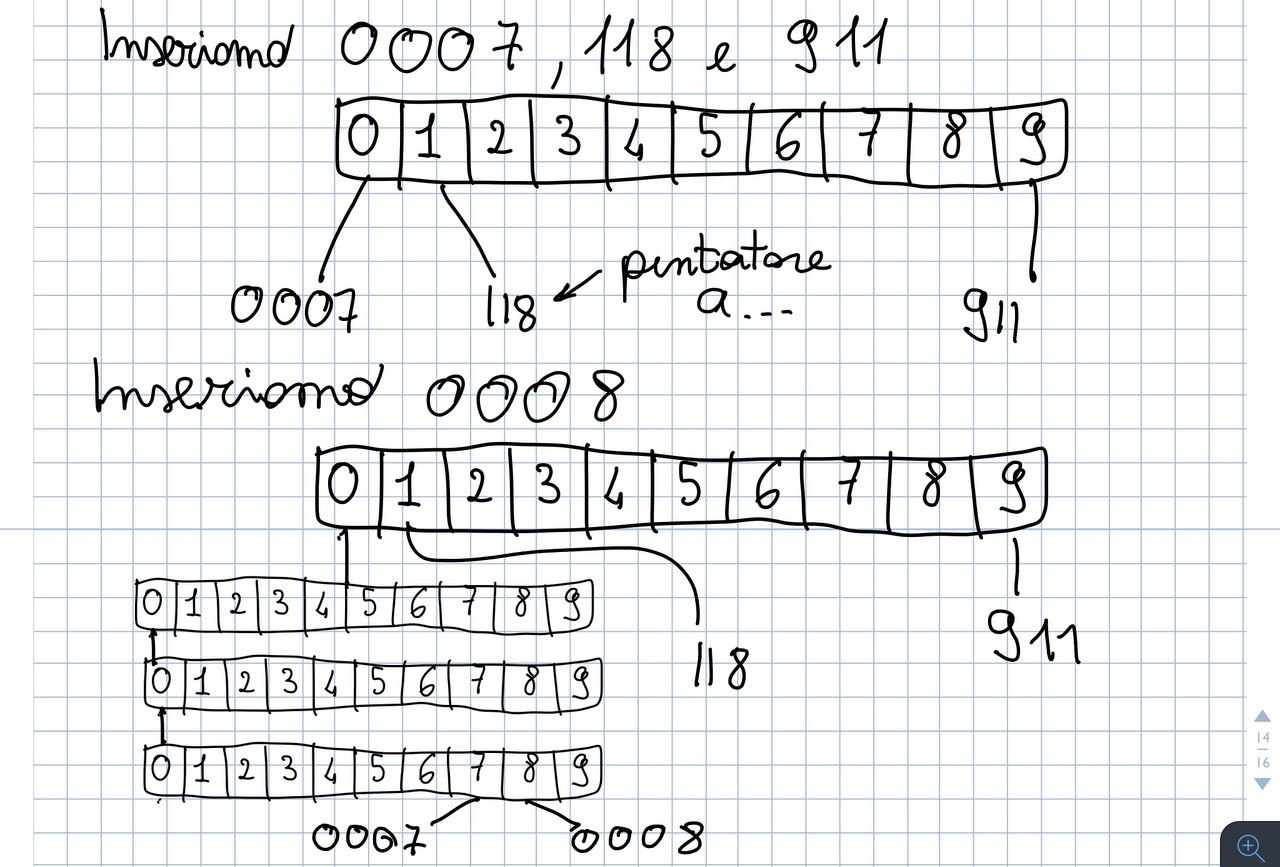
\includegraphics[width=\linewidth]{Trie.jpg}
\end{figure}

Ogni nodo che viene creato occupa uno spazio che è $O(\sigma)$ e ne vengono creati d interni in più abbiamo n puntatori alle stringhe. Quindi in tutto portano uno spreco di memoria pari a $O(n+d*\sigma)$. La complessità in tempo necessaria per creare il trie è pari a $O(n+d*\sigma)$.

Possiamo provare a ridurre lo spazio necessario per mantenere tutta la struttura che ci permette di visitare l'albero da sinistra verso destra per ottenere un ordinamento della stringa.
Al posto degli array che mi occupano sempre $O(\sigma)$ possiamo usare una hash table in cui però il numero delle entry è pari a $e_u$ ed è proporzionale al numero di archi che escono dalla tabella hash. 
In nodi interni sono sempre d quindi abbiamo un costo $O(d)$ per creare tutti i nodi della struttura, poi l'aggiunta di un nuovo arco nei vari nodi mi costa $O(1)$.
Il problema è che le tabelle hash non sono ordinate, quindi ogni tabella hash va prima ordinata e poi va fatta la visita da sinistra a destra.
Ogni singola hash table va ordinata e questo mi costa
\newline
$\sum_u e_u Log e_u$ ovvero $(\sum_u e_u) Log \sigma$ che diventa $O(d Log \sigma)$.

Lo spazio occupato utilizzando MSD con le tabelle hash è pari a $O(d+n)$ perchè dobbiamo allocare tutti i puntatori per i nodi interni e poi abbiamo le foglie.

Il tempo invece è $O(d Log \sigma)$ che non è ottimo ma almeno abbiamo guadagnato molto in spazio.

Una alternativa all'utilizzo delle hash table consiste nell'uso dei compacted trie (spiegati in seguito) in cui riduciamo il numero dei nodi interni che diventano al più n, come il numero delle foglie. Quindi la complessità diventa in spazio $O(n+n)$ perchè abbiamo n nodi interni e n foglie mentre il tempo sarà $O(d+nLog\Sigma)$.

\section{Multi-Key QuickSort}

Si tratta dell'estensione del classico algoritmo QuickSort visto in precedenza, in questo caso non vogliamo solamente ordinare elementi atomici ma elementi di lunghezza variabile, come le stringhe.
Anche in questo caso si utilizza il pivot scelto random, qua il pivot è una stringa del nostro set di stringhe da ordinare e, in particolare, ad ogni esecuzione del Multi-Key Quicksort il pivot non è tutta la stringa ma solamente un carattere della stringa che ci consente di partizionare il set di stringhe R.
La richiesta è che il set di stringhe R sia fatto in modo che nessuna delle stringhe sia un prefisso delle altre.
Il codice di Multi-Key Quicksort:
\begin{code}
\begin{lstlisting}[escapeinside={(*}{*)}]
if |R| $\leq$ 1:
    return R
else:
    scegliere un pivot p in R
    $R_<$ = {s: s[i]<p[i]}
    $R_=$ = {s: s[i]=p[i]}
    $R_>$ = {s: s[i]>p[i]}
    A = Multi-KeyQuicksort($R_<$, i)
    B = Multi-KeyQuicksort($R_=$, i+1)
    C = Multi-KeyQuicksort($R_>$, i)
    
    return A+B+B
\end{lstlisting}
\end{code}

La precodizione del'algoritmo e di tutte le chiamate ricorsive è che nel momento in cui scegliamo la stringa s come pivot e prendiamo l'indice i da usare all'interno della stringa pivot, i precedenti $(i-1)$ caratteri siano già ordinati.
Da notare che faccio tre chiamate ricorsive a Multi-KeyQuicksort, in particolare in due occasioni non viene neanche aumentato il valore di i mentre una volta si. Se sono nel caso $R_<$ e $R_>$ non va aumentato i perchè anche l'elemento in posizione i va di nuovo confrontato, infatti questo elemento era uguale all'elemento in posizione i del pivot ma potrebbe essere differente rispetto agli altri elementi in posizione i dello stesso set.
Invece nel caso $R_=$ non confronto l'elemento i perchè sappiamo già che è uguale e si passa direttamente all'(i+1).

Contiamo il numero di confronti che vengono effettuati per ognuna delle stringhe. Quando facciamo un confronto una stringa ha due possibilità:
\begin{itemize}
\item O finisce in $R_<$ e $R_>$ e in questo caso non viene modificata la i. Se la selezione dei pivot è buona e le stringhe vengono distribuite nel modo corretto abbiamo che $|R_< \cap R_>| < \frac{\alpha}{n}$ dove $\alpha$ è un valore minore di 1, quindi in pratica vuol dire che la dimensione del set viene diminuita di un fattore costante ad ogni iterazione, ovvero viene ridotta $log_2 n$ volte.
\item La stringa finisce in $R_=$ e in questo caso abbiamo un aumento della i che quindi porta una diminuzione del numero di confronti rimasti da fare. Dato che la stringa è lunga $|s|$ vuol dire che al più possiamo fare s confronti. Questo valore può essere raffinato se pensiamo al fatto che in ogni stringa abbiamo un numero di caratteri $d_s$ che mi permette di distinguere la stringa dalle altre e quindi non dovrò fare $|s|$ confronti ma solamente $d_s$. 
\end{itemize}

Considerando non solo una stringa ma n stringhe, abbiamo che il numero di confronti da effettuare in tutto diventa $O(n(d_s + Logn)) = O(d+nLogn)$.

\subsubsection{Ternary Trees}

Possiamo fare un parallelismo tra l'idea del multi-key quicksort che divide le stringhe in tre set e l'idea del Ternary tree, un albero in cui i vari nodi possono avere al più tre figli fatti in questo modo, in ogni nodo abbiamo un certo carattere e poi possiamo avere tre figli, in un ramo mettiamo quelle stringhe che hanno il carattere minore del nodo padre, in uno gli uguali e in uno i maggiori.
In un albero ternario di questo tipo, così come nel MK Quicksort quando scendiamo a sinistra o destra di un nodo non aumentiamo la i che indica l'elemento da confrontare, l'aumento invece avviene quando prendiamo il ramo uguale.
La ricerca di ua stringa lunga p in un albero di questo tipo avviene eseguendo al più $O(Logn + p)$ confronti.
Un esempio di Ternary Search Tree, costruzione e ricerca:

\begin{figure}[]
\centering
  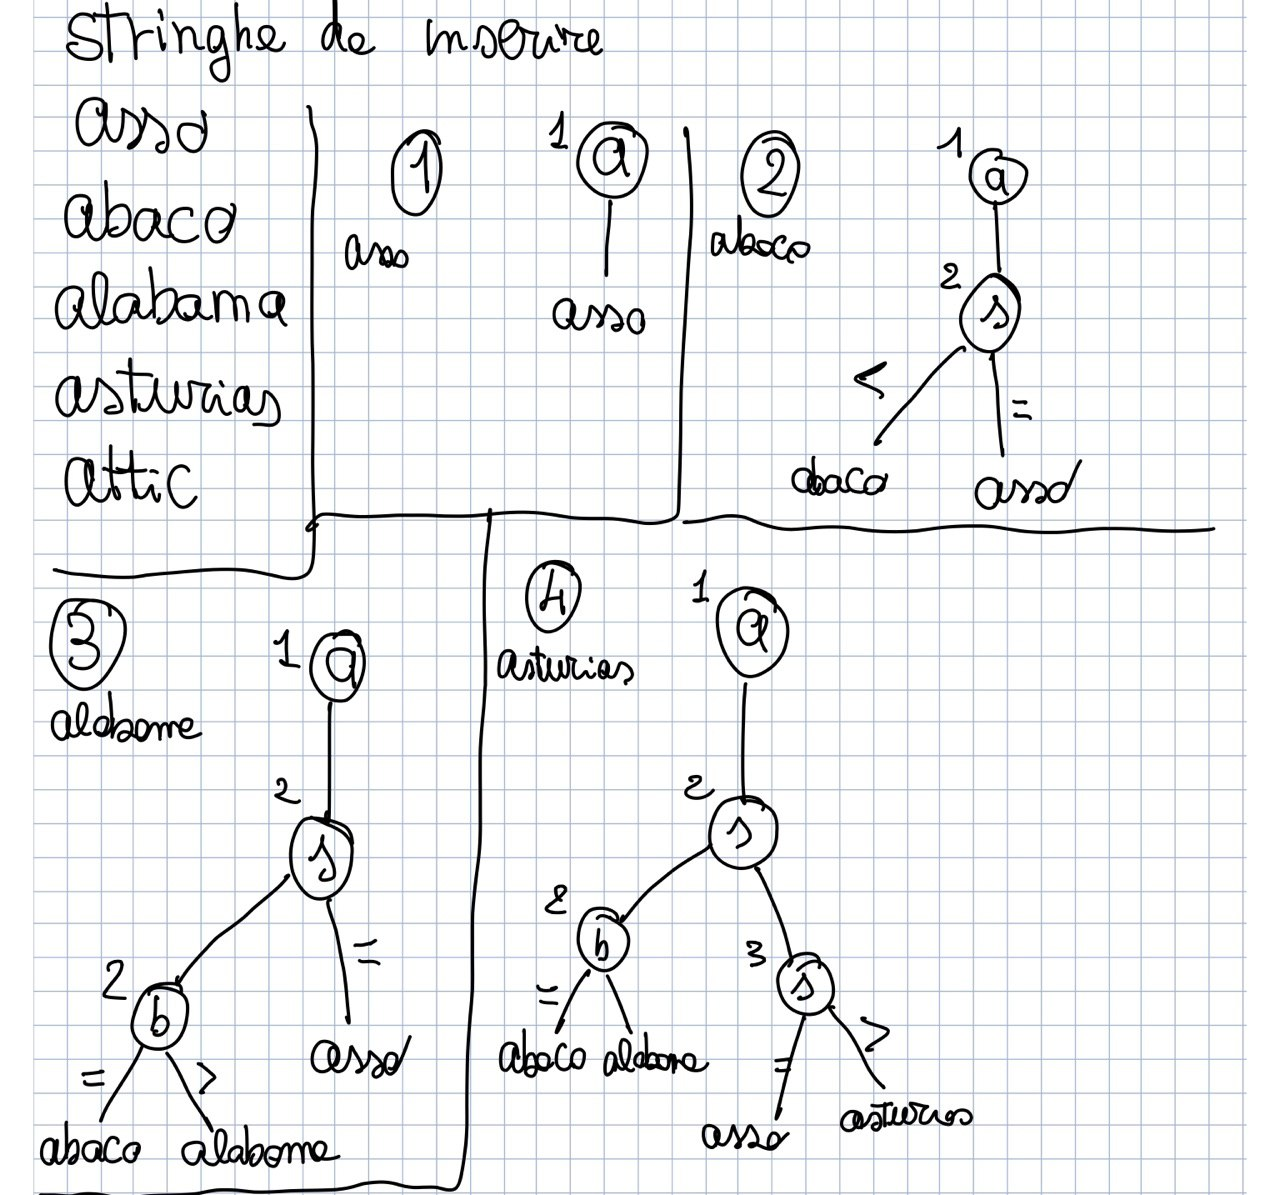
\includegraphics[width=0.85\linewidth]{Es1Trie.jpg}
\end{figure}

\begin{figure}[H]
\centering
  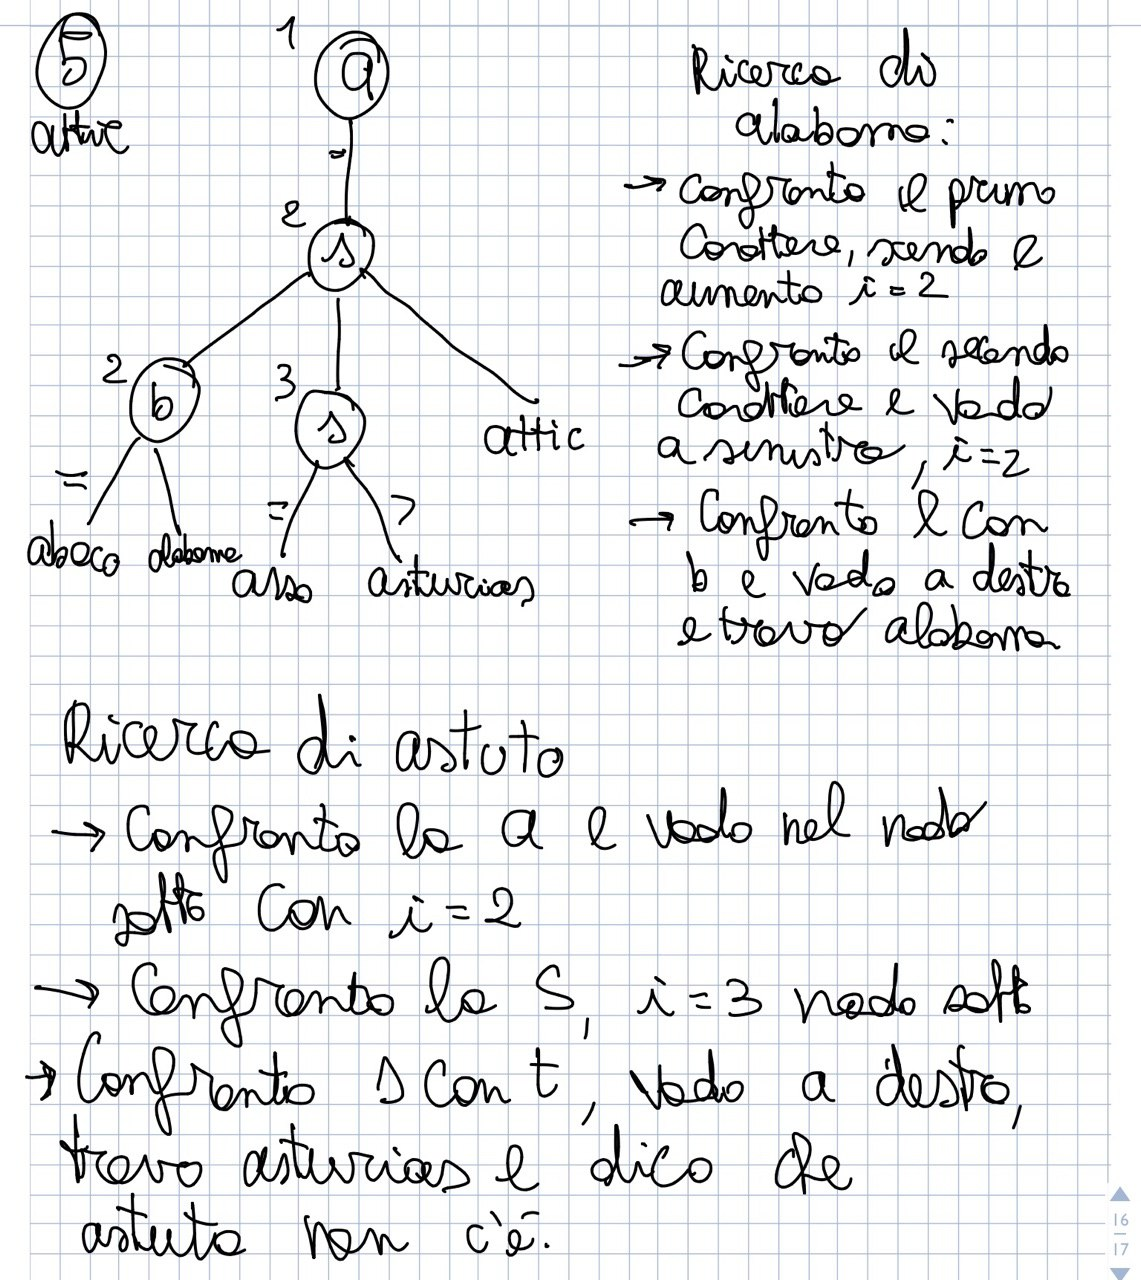
\includegraphics[width=0.85\linewidth]{Es2Trie.jpg}
\end{figure}
\newpage
\section{Ordinamento di stringhe con l'I/O Model (Probabilmente non va fatta)}

Il sorting delle stringhe usando il 2 level model è molto più complicato rispetto al sorting delle stringhe in memoria interna.
La difficoltà sta soprattutto nel fatto che il confronto brute force delle stringhe può comportare un alto numero di operazioni di I/O, inoltre avere delle stringhe di lunghezza variabile non rende più semplice il tutto.
Lavorando nel 2 level model, le stringhe possono essere divise in due tipologie:
\begin{itemize}
\item Stringhe che hanno una lunghezza minore del valore B del blocco di dati che posso portare in memoria, ne abbiamo un numero $n_s$ e in tutto hanno una lunghezza $N_s$.
\item Stringhe che hanno una lunghezza maggiore di B, sono $n_l$ e in tutte hanno una lunghezza $N_l$.
\end{itemize}
Il numero totale di stringhe è $n=n_s+n_l$ mentre la lunghezza totale delle stringhe è $N = N_l + N_s$.

Per l'ordinamento delle stringhe in memoria ci sono 3 modelli differenti e ognuno comporta una differente complessità in termini di I/O:

\begin{itemize}
\item Un primo modello considera le stringhe indivisibili (non divide in caratteri) e le divide solamente quando le deve portare in memoria se la lunghezza è maggiore di B.
\item Un secondo modello invece divide le stringhe in caratteri ma solamente quando sono in memoria interna
\item Un terzo modello invece divide le stringhe in caratteri sia quando le stringhe sono in memoria interna sia quando non sono in memoria interna.
\end{itemize}




\chapter{Prefix Search di Stringhe}

Il problema è il seguente:
\newline
\textit{Abbiamo un dizionario D con n stringhe, la somma totale della lunghezza delle stringhe è N. Dato il prefisso P dobbiamo cercare all'interno del dizionario quelle stringhe che hanno P come prefisso (possiamo contarle o restituirle).}

Il problema si presenta, ad esempio, quando si deve usare l'auto completion nei motori di ricerca perchè l'utente quando scrive una query ottiene anche dei suggerimenti basati su quello che ha scritto e anche su quello che gli altri utenti cercano.

\section{Soluzione con array di puntatori}

Una prima soluzione, semplice ma non buona dal punto di vista dell'efficienza consiste nell'utilizzo di:
\begin{itemize}
\item Un array A di puntatori alle stringhe
\item Il dizionario D delle stringhe vere e proprie
\end{itemize}

Le stringhe possono essere su disco e non sono ordinate e non si trovano una vicina all'altra. Nell'array A dei puntatori alle stringhe invece le varie stringhe sono ordinate.
L'array A deve soddisfare due proprietà:
\begin{itemize}
    \item In A le stringhe che hanno il prefisso in comune si trovano vicine tra loro. Quindi tutte le stringhe che hanno come prefisso P hanno i puntatori nel range A[l,r].
    \item La stringa P la troviamo tra A[l-1] e A[l].
\end{itemize}

Vista la prima delle due proprietà quello che vorremmo fare è trovare i due delimitatori l ed e e quindi in questo modo calcolare il numero di stringhe prefisse da P ed eventualmente ottenere le stringhe.
L'idea quindi è di ridurre il problema ad un problema di ricerca lessicografica di Q = {P,P\#} all'interno del dizionario di stringhe D utilizzando una ricerca binaria. Q viene formato considerando il pattern P che quindi nella ricerca sarà prima di tutti e ci restituirà l'indice l e poi il pattern P\# dove \# indica un carattere più grande di qualsiasi altro carattere dell'alfabeto, questo ci restituirà l'indice r+1.

Quindi preso Q andiamo ad eseguire una ricerca binaria all'interno del set D di stringhe, vengono eseguite $O(Logn)$ ricerche e in ognuna di queste ricerche vengono confrontati un numero di caratteri che è pari a O(p). Quindi, per ottenere il numero di stringhe che hanno come prefisso P abbiamo un costo in tempo che è $O(pLogn)$, un numero di operazioni di I/O pari a $O(\frac{p}{B}Logn)$. Lo spazio occupato è $O(N+(1+w)n)$ bytes perchè abbiamo le stringhe di lunghezza complessiva N e poi abbiamo i puntatori alle stringhe e ognuno dei puntatori ha lunghezza w.
Se invece vogliamo ottenere non il numero delle stringhe ma le stringhe vere e proprie non mi basta calcolare $r-l+1$ che richiede $O(1)$ ma devo accedere a tutte le stringhe, quindi il numero di operazioni I/O sale a $O(\frac{p}{B}Logn\ +\ #Noccorrenze)$ = $\Omega(n_{occ})$.

\subsection{Migliorare l'efficienza: 2 level Indexing}

Una prima idea per migliorare l'efficienza consiste nel cercare di diminuire il numero di operazioni I/O che devono essere effettuate nel momento in cui dobbiamo recuperare le stringhe che hanno come prefisso P. In precedenza avevamo detto che questo aveva un costo in termini di I/O pari a $\Omega(n_{occ})$.

Per diminuire questo costo ordiniamo le stringhe lessicograficamente anche in memoria, in questo modo abbiamo l'array A con i puntatori che è ordinato e poi in memoria abbiamo il dizionario D che ha tutte le stringhe ordinate e messe una dopo l'altra.
Questo è comodo sia perchè può comportare una diminuzione dello spazio occupato nel caso in cui si vada ad utilizzare un algoritmo di compressione sia perchè quando eseguirò la ricerca binaria su una parte di questi dati, probabilmente le stringhe vicine verranno portare in memoria e quindi non dovrò andare nel disco a prenderle risparmiando tempo.

Come funziona quindi:
\begin{itemize}
\item Prendiamo il dizionario D e lo dividiamo in blocchi di B caratteri, in questo modo creiamo $n_b = \frac{N}{B}$ blocchi, in A andiamo a mettere i puntatori alla prima stringa di questi $n_b$ blocchi.
\item La ricerca va modificata, abbiamo sempre Q = {P,P\#}, prima andiamo a fare la ricerca di Q tra le $n_b$ posizioni che sono state prese come sample e poi nel momento in cui troviamo queste posizioni eseguiamo la ricerca all'interno dei blocchi in cui sono le nostre stringhe prefisse.
\end{itemize}

Quindi, il numero di operazioni I/O ora diventa $O(\frac{p}{B}Log\frac{N}{B})$ perchè la ricerca binaria ora avviene tra $\frac{N}{B}$ elementi. Se poi dobbiamo ottenere le stringhe e non solamente il conteggio delle stringhe prefisse allora, considerato che le stringhe ora ordinate anche nel disco e chiamando $N_{occ}$ il numero dei caratteri delle stringhe che dobbimao restituire, possiamo dire che il numero di I/O si riduce a $O(\frac{N_{occ}}{B})$. 
Lo spazio utilizzato si riduce a $O(N+\frac{N}{B})$ perchè abbiamo sempre N stringhe ma ora i puntatori sono ridotti ai soli puntatori verso le stringhe sample.

\subsection{Front Coding}

Data una sequenza di stringhe ordinate, è probabile che alcune di queste stringhe abbiano in comune con la precedente un prefisso P, quindi potrebbe essere una buona idea applicare una compressione delle stringhe senza ripetere ogni volta il prefisso in comune con la stringa precedente.
È quello che si fa con il Front Coding, in questo algoritmo di compressione l'idea è quella di prendere i primi l caratteri di una stringa in comune con la precedente che occupano $lLog\sigma$ bit sostituendoli con $log_2 l$ bit.
La regola è la seguente:
Ogni stringa viene sostituita con una coppia $<l,s_i>$ in cui l indica il numero di caratteri in comune con la stringa precedente e $s_i$ indica i caratteri che non sono in comune e che sono nella seconda stringa. Durante la decodifica devo prendere gli l caratteri della stringa precedente e metterci dopo i caratteri $s_i$ che ho messo nella rappresentazione codificata della stringa. La decodifica mi costa $O(|s|)$ ma può essere un problema quando abbiamo una sequenza di molte stringhe perchè per codificare una certa stringa potrei dover arrivare all'inizio della sequenza.
Quindi un'idea che si sposa bene con l'allocazione continua delle stringhe vista in precedenza è la divisione delle stringhe in blocchi di dimensione B, in questo modo la prima stringa del blocco ha $l=0$ quindi viene memorizzata completamente e il resto è compresso.
Questo è comodo anche perchè nel momento in cui andiamo a creare l'array con i vari puntatori inseriamo un numero di puntatori che non sarà più $\frac{N}{B}$ ma sarà $\frac{FCB(D)}{B}$ dove FCB(D) indica la versione compressa di D, quindi in pratica ho meno puntatori e la ricerca binaria la faccio tra meno elementi.
In più questo mi permette di andare a fare la scansione del blocco in cui sono le stringhe prefisse andando contemporaneamente a scansionare (controllando se la stringa è prefissa) e decodificando.
Quindi:

\textbf{La prefix search richiede $O(\frac{P}{B}Log\frac{FCB(D)}{B})$} operazioni di I/O se vogliamo solamente contare il numero di occorrenze e invece ne richiede $\frac{FCB(D_{occ}}{B}$ se vogliamo proprio le stringhe dove $D_{occ}$ indica l'insieme delle stringhe che devono essere restituite.

Un problema può avvenire con alcune stringhe in particolare ($<0,a>,<1,a>,<2,a>$) e questo può comportare la salita del tempo necessaio per decodificare un blocco di B elementi da $O(B)$ a $O(B^2)$. 
Bisogna considerare bene la scelta di B:
\begin{itemize}
\item Con un valore di B molto grande abbiamo un'ottima compressione, dimuniscono le stringhe non compresse e quindi dimunisce la dimensione dell'array dei puntatori. Al contrario però sale il tempo necessario allo scan del blocco di dimensione B.
\item Con un valore di B piccolo, aumentano le stringhe non compresse, quindi aumenta l'array con i puntatori che potrebbe anche non entrare in memoria interna, però allo stesso tempo diminuisce il tempo necessario per eseguire la scansione dei sub array di dimensione B. Peggiore anche la compressione.
\end{itemize}

\section{Interpolation Search}

Se ci troviamo in presenza di un array che rispetta alcune caratteristiche statistiche possiamo sfruttare l'interpolation search per eseguire una ricerca all'interno dell'array.
L'idea è che questo metodo possa essere utilizzato sia con un array di interi ma possa essere soprattutto esteso alla ricerca di stringhe andando a rappresentare le stringhe come numeri interi in modulo.

La preconzione di questo algoritmo di ricerca è che l'array in cui vogliamo fare la ricerca sia ordinato, in particolare dato l'array $X[1,m]$ è necessario che $x_i > x_{i-1}$.
Come funziona l'algoritmo, vediamo come preparare l'array per la ricerca:
\begin{itemize}
\item È necessario dividere l'array in un numero di bin pari al numero m di elementi presenti all'interno dell'array. Ad esempio se abbiamo un array con 12 elementi (m=12) avremo un numero di bin pari a 12 $(B_1,...,B_12)$.
\item Ognuno dei bin avrà una lunghezza $b=\frac{x_m-x_1+1}{m}$
\item Calcoliamo i delimitatori dei bin non andando a calcolare la posizione in cui si devono trovare il punto d'inizio e di fine ma andando a vedere il range di elementi che si troveranno all'interno del bin. Questo comporta che alcuni bin potrebbero essere vuoti, ad esempio se ho un array con elementi 1,2,3,7,8 e voglio bin lunghi al massimo 3, posso creare un primo bin con 1,2,3 poi non avrò il secondo bin perchè magari sarebbe formato da 4,5,6 e quindi passo subito al terzo bin. In particolare la formula per calcolare i delimitatori dei bin è la seguente $B_i=[x_1+(i+1)b, x_1+ib]$.
\end{itemize}

La suddivisione in bin porta anche la necessità di avere un array di $O(m)$ elementi in cui andiamo a salvare i puntatori ai vari punti dell'array in cui iniziano i vari bin.

Per fare la ricerca all'interno dell'array faccio così:
\begin{itemize}
\item Calcoliamo il bin in cui dovrebbe trovarsi l'elemento y che cerchiamo, $j = \frac{x_y-x_1}{b} + 1$. 
\item Al secondo step andiamo a prendere il bin in cui potrebbe stare l'elemento ed eseguiamo una ricerca binaria all'interno del bin.
\end{itemize}

Il costo dell'algoritmo quindi è in spazio $O(m)$ perchè abbiamo l'array con i puntatori, e in tempo è $O(Log b)$ ($O(Log \Delta)$) perchè facciamo la ricerca binaria in array lunghi b elementi.

Teorema: La ricerca costa $O(Log \Delta)$ dove $\Delta$ è la media tra il massimo e il minimo gap tra due elementi consecutivi dell'array

\textbf{Dimostrazione:} Per dimostrare la complessità in tempo consideriamo che il massimo gap tra due interi presenti nell'array è maggiore della media degli elementi presenti nell'array:

\begin{equation}
    max_{i=2,..}(x_i-x_{i-1}) \geq \frac{\sum_{i=2}^m x_i - x_{i-1}}{m-1} \geq \frac{x_m - x_1 + 1}{m} = b
\end{equation}

Il numero massimo di elementi di ogni bin invece dipende dal fatto che gli elementi dell'array sono divisi da un numero di $s= min_{i=2...m}(x_i-x_{i-1})$ e quindi il numero di elementi di ogni bin diventa $\frac{b}{s}$.
Quindi considerando tutte le precedenti disuguaglianze possiamo scrivere:

\begin{equation}
    |B_i| \leq \frac{b}{s} \leq \frac{max_{i=2,..}(x_i-x_{i-1}) }{min_{i=2...m}(x_i-x_{i-1})} = \Delta 
\end{equation}

Note:
\begin{itemize}
\item Il caso pessimo lo abbiamo se tutti gli elementi finiscono in un bin e in questo caso avremmo una complessità che è $Log m$
\item L'algoritmo è cache oblivious
\item L'occupazione in spazio è $O(m)$ cosa che non è necessaria in una classica binary search

\end{itemize}

Se gli interi dell'array sono distribuiti in modo uniforme, l'algoritmo richiede un tempo $O(Log Log m)$ con alta probabilità.

\textbf{Dimostrazione:} Partiamo dicendo che abbiamo una distribuzione uniforme di interi e quindi ogni bucket contiene $O(1)$ intero. 
Assumiamo di partizionare gli interi in un numero di range pari a $r=\frac{m}{2Logm}$. Con probabilità $\frac{1}{r}$ un intero è in un range e con probabilità $(1-\frac{1}{r})^m = (1-\frac{m}{2Logm})^m = O(e^{-2Logm}) = O(\frac{1}{m^2})$ abbiamo un range che non contiene neanche un intero.
Se diciamo che ogni range contiene almeno un elemento allora la distanza massima tra due interi vicini nell'array dovrà essere minore di 2 volte la lunghezza del range, quindi $max_i(x_i-x_{i-1})=\frac{2U}{r}=O(\frac{ULogm}{m})$.
Se prendiamo $r' = \Theta(mLogm)$ range possiamo dire che ogni coppia di range vicini tra loro contengono almeno un intero (se sta in un range poi nei due vicini potrei non avere interi).
Quindi il gap minimo tra due interi della sequenza può essere limitato in questo modo: $min_i(x_i-x_{i-1})\geq \frac{U}{r'} = \Theta(\frac{U}{mLogm})$.
Ora prendiamo i due risultati e calcoliamo la divisione:
\begin{equation}
    \Delta = \frac{ULogm}{m}*\frac{mLogm}{U} = O(Log^2 m)
\end{equation}

Questo è il delta che volevamo calcolare che ci indica che se gli interi sono distribuiti in modo random allora il costo per l'interpolation search che di norma è $O(Log \ dimensione\ bin) = O(Log \Delta) = O(Log Log m)$.

\section{Locality Preserving Front Coding}

Si tratta di una versione migliorata del classico Front Coding, in questo caso l'idea è di andare a comprimere solamente quelle stringhe che poi vengono decompresse in tempo ottimo lasciando le altre non compresse.
Utilizzare questa tecnica diminuisce il tempo per la decodifica e migliora anche lo spazio occupato dalle stringhe compresse.
Come si comprime, data una sequenza di stringhe:
\begin{itemize}
\item Consideriamo la stringa S, andiamo a sinistra di $c|S|$ e vediamo se in questo intervallo troviamo una stringa copiata
\item Se troviamo una stringa copiata che è interamente contenuta nell'intervallo allora possiamo scrivere la stringa S comprimendola con front coding, altrimenti se una stringa finisce nell'intervallo o non ci sono stringhe nell'intervallo allora dobbiamo copiare la stringa S senza usare il front coding.
\end{itemize}

Le stringhe copiate sono tali che andando a sinistra di $C|S|$ non si trova un'altra stringa copiata (intera).

\textbf{Teorema}: Utilizzando il Locality Preserving Front Coding si consuma $O((1+\epsilon)FC(D))$ spazio e un numero di operazioni I/O pari a $O(\frac{FC(D)}{\epsilon B})$.

Dimostrazione: Consideriamo prima le stringhe che sono salvate compresse, quindi lo spazio che occupano è limitato superiormente da $FC(D)$. Le stringhe che invece sono copiate le dividiamo in due gruppi:
\begin{itemize}
\item Stringhe copiate Uncrowded: sono quelle stringhe che a sinistra hanno una quantità di caratteri Front coded maggiore di $\frac{C|S|}{2}$;
\item Stringhe copiate Crowded: sono quelle stringhe che a sinistra hanno una quantità di caratteri Front coded minore di $\frac{C|S|}{2}$;
\end{itemize}

Da questa relazione possiamo dire che per una stringa s' copiata che viene prima di una stringa crowded, vale la seguente relazione: $|s'| \geq \frac{C|S|}{2}$.

Ora creiamo delle sequenze tali che la prima stringa è uncrowded e poi dopo c'è la massima sequenza di stringhe crowded. 
Possiamo dire che, prendendo una stringa crowded $w_i$ si verifica la seguente relazione:
\begin{equation}
|w_{i-1}| > \frac{C|w_i|}{2} \ ovvero \ |w_{i}| < \frac{2|w_{i-1}|}{C} < (\frac{2}{C})^2|w_{i-2}| < (\frac{2}{C})^3|w_{i-3}|
\end{equation}
\begin{equation}
< (\frac{2}{C})^{i-1}|w_{1}|
\end{equation} 

Facciamo la sommatoria

\begin{equation}
\sum_{i=0}^x  (\frac{2}{C})^{i-1}|w_{1}| = \frac{c}{c-2}|w_i|
\end{equation}

Ora consideriamo la stringa uncrowded $w_1$ che è preceduta da una serie di caratteri Front coded maggiori di $\frac{C|w_1|}{2}$ e questo valore è limitato da FC(D).
Quindi abbiamo
\begin{equation}
\frac{C|w_1|}{2} < FC(D) \ => |w_1| < \frac{2FC(D)}{C}
\end{equation}

Ora sostituiamo questo secondo valore nel primo e otteniamo:
\begin{equation}
\frac{c}{c-2}\frac{2FC(D)}{C} = \frac{2FC(D)}{C-2}
\end{equation}
Per $\epsilon = \frac{2}{C-2}$ vale il teorema.

\section{Trie}



\begin{figure}[h!]
\centering
  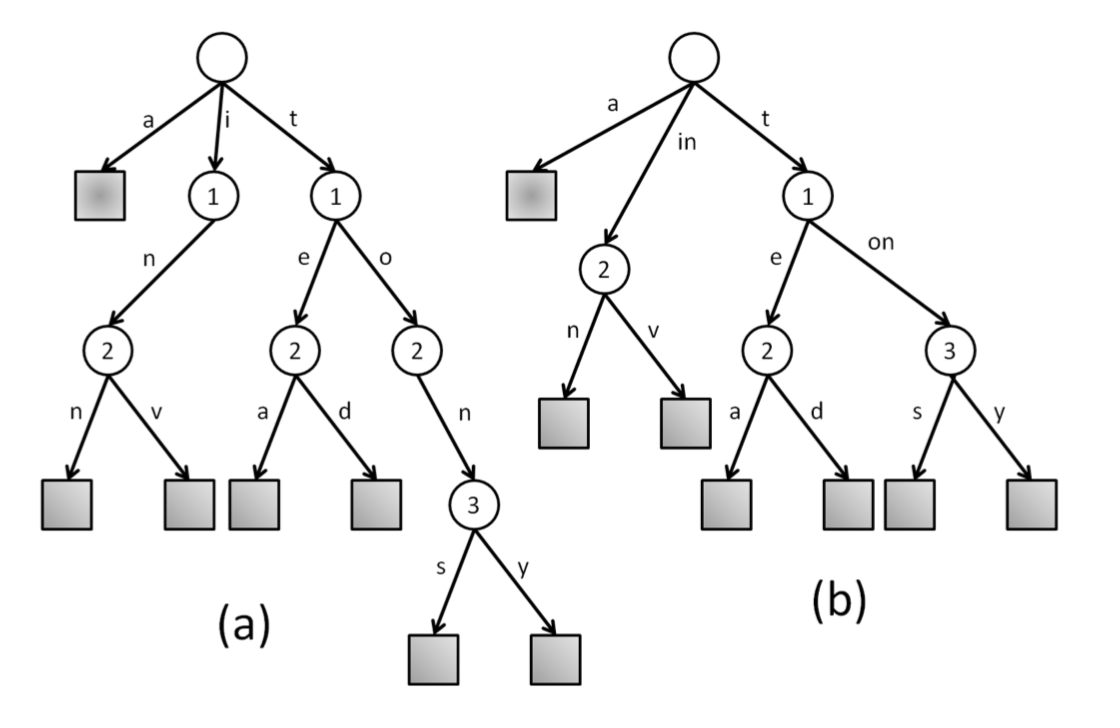
\includegraphics[width=0.5\linewidth]{CompUnc.png}
  \caption{Un Uncompacted trie a sinistra e il compacted a destra.}
  \label{}
\end{figure}

\subsection{Uncompacted Trie}

Un Uncompacted trie è un albero in cui da ognuno dei nodi possono uscire più archi, ognuno dei nodi interni è associato ad una stringa $s[u]$ che creiamo andando dal nodo root a u, questa stringa sarà prefissa di tutte le stringhe che possiamo raggiungere a partire dal nodo u. Questo tipo di albero è chiamato uncompacted perche è possibile avere dei percorsi formati da nodi unari ovvero da nodi che hanno solamente un arco in uscita. Il numero delle foglie è n, quante le stringhe, il numero dei nodi interni è N e dipende dalla lunghezza totale delle stringhe.
Il problema sta nel decidere la struttura dati da utilizzare per memorizzare i nodi, in particolare per ogni nodo devo salvarmi quali sono gli archi uscenti:
\begin{itemize}
\item Possiamo utilizzare una lista linkata, in questo caso se dobbiamo fare una ricerca del prefisso P e ci troviamo nel nodo, dobbiamo scorrere la lista e quindi potremmo avere un costo $O(\sigma)$ che diventa $O(p\sigma)$ per per cercare p caratteri
\item Possiamo usare un array ordinato, in questo caso eseguiamo una ricerca binaria e quindi alla fine in $O(pLog\sigma)$ troviamo l'arco da seguire.
\item Possiamo usare un array con $\sigma$ elementi in cui quelli che hanno un arco uscente hanno un puntatore, la ricerca all'interno di questo array mi costa $O(1)$ e quindi nel complesso la ricerca del prefisso P mi costa $O(P)$. Il problema qua è che ho una occupazione di spazio pari a $O(N\sigma)$.
\item La soluzione migliore è utilizzare una hash table perfetta in cui abbiamo la ricerca in $O(P)$ e una complessità in spazio che è ottima.
\end{itemize}

Teorema: L'uncompacted Trie risolve il problema del Prefix Search in $O(P+n_{occ})$ tempo dove $n_{occ}$ è il tempo necessario per trovare le occorrenze delle stringhe e quindi contarle, il numero di operazioni I/O necessarie è $O(P+\frac{n_{occ}}{B})$. Se oltre al numero di stringhe che hanno quel prefisso vogliamo trovare anche le stringhe allora abbiamo un costo I/O aggiuntivo pari a $\frac{O(N_{occ}}{B})$ dove $N_{occ}$ è la lunghezza delle stringhe da restituire.
Il tutto supponendo che le stringhe sono salvate ordinate in memoria e sono una vicina all'altra.

\subsection{Compacted Trie}

Dato che un uncompacted trie può sprecare molto spazio perchè abbiamo sempre una complessità $O(N+n)$, si può comprimere l'uncompacted trie in un compacted trie che permette di ridurre l'occupazione di spazio a n nodi interni + n nodi relativi alle stringhe, quindi complessivamente $O(n)$.
Nel compacted Trie vengono rimossi i percorsi unari e quindi abbiamo degli archi in cui non c'è più un solo carattere ma la stringa prefissa al nodo. Questo può essere un problema perchè avere sugli archi del nodo u la stringa prefissa alle stringhe che raggiungo da u può comportare un alto consumo di spazio.
Per risolvere il problema si cerca di rendere la rappresentazione più compatta andando a sostituire la stringa prefissa con una tripla $<ID stringa, inizio, lunghezza>$.
In questo modo utilizzo sole 3 parole di memoria ovvero 12 byte che non influisce sulla complessità perchè è una costante.
Alla fine lo spazio necessario per memorizzare gli archi diventa $O(n)$.
Teorema: Il compacted Trie risolve il problema del prefix search in $O(P+n_{occ})$ e con $O(p+\frac{n_{occ}}{B})$ I/O.
Ottenere le stringhe costa un tempo $O(N_{occ})$ e un numero di I/O pari a $\frac{N_{occ}}{B}$. Lo spazio occupato dal compacted Trie è $O(n)$ contro $O(N)$ dell'uncompacted.

Il compacted Trie può essere utilizzato anche per una ricerca lessicografica di una stringa perchè cerco la stringa nel trie e poi mi fermo quando ho un mismatch e capisco quale sarebbe la posizione della stringa e dove andrebbe inserita eventualmente.

\section{Patricia Trie}

Si tratta di una evoluzione del compacted Trie in cui per ogni arco non viene salvata una tripla ma solamente un carattere che è il primo del prefisso, poi all'interno del nodo collegato a quell'arco viene inserito un numero che indica la lunghezza della stringa associata fino a quel nodo.
Anche questo Patricia Trie è in grado di supportare la ricerca di un pattern P tra varie stringhe ma la tecnica utilizzata è differente e si utilizza un algoritmo chiamato Blind Search:
\begin{itemize}
\item Abbiamo a disposizione un pattern P da cercare, viene eseguita la ricerca di questo pattern all'interno del patricia trie e si arriva ad una foglia l in cui troviamo una stringa che è interessante rispetto al pattern (perchè rappresenta l'ultima stringa che ha un prefix in comune con P).
Durante la scansione del patricia trie dall'alto verso la foglia troviamo una serie di caratteri che possono essere in comune e poi ad un certo punto arriviamo ad un carattere che invece segna un primo mismatch. Quindi diciamo che, se arriviamo in una foglia che punta ad una stringa che chiamiamo C, ci saranno n caratteri di s in comune con P ovvero $P[1,n]=C[1,n]$ e poi avremo $P[n+1]\ != \ C[n+1]$.
\item La seconda fase è una visita dal basso all'alto, si parte dalla foglia l che punta alla stringa C e si va verso l'alto fino a che non troviamo che l'arco $e=(u,v)$ tale che $S[u] < l < S[v]$ ovvero il numero scritto nel nodo deve essere minore o uguale a l in tal caso ci fermiamo.
Una volta trovato l'arco (u,v) abbiamo due possibilità:
\begin{itemize}
\item $S[u]=l$, in questo caso tutte le stringhe che sono sotto al nodo u hanno come lcp (longest common prefix) il prefisso P[1,l]. Per trovare la posizione lessicografica di P devo vedere tutti gli archi uscenti da u e appena ne trovo uno in cui il carattere $l+1$ è maggiore di $P[l+1]$ allora dico che la posizione di P è a sinistra di questo arco.
\item Se invece il mismatch è a metà tra $S[u]$ e $S[v]$ allora posso dire che le foglie che stanno nel sottoalbero che inizia in v hanno tutte come lcp $P[1,l]$. 
Per trovare la posizione lessicografica di P poi ci sono due casi:
\begin{itemize}
\item Se $P[l+1] < S[l+1]$ allora la posizione di P è a sinistra del sottoalbero che esce da V
\item Se $P[l+1] > S[l+1]$ allora la posizione di P è a destra del sottoalbero che esce da V
\end{itemize}
In entrambi i casi la posizione lessicografica di P è adiacente al sottoalbero che esce da V.
\item 
\end{itemize}
\end{itemize}

\textbf{Teorema:} Un Patricia Trie permette di eseguire la ricerca di un pattern P[1,p] in tempo $O(p)$ con un consumo di spazio che è $O(n)$ e un numero di operazioni I/O che è pari a $O(\frac{p}{B})$ e che vengono utilizzate per comparare la stringa identificata dall'algoritmo blind search.
Se $n<M$ possiamo far entrare in memoria tutto il Patricia trie, occuperò sempre $O(n)$ in memoria e poi avrò $O(N)$ per l'occupazione nella memoria esterna.

Possiamo anche utilizzare il Patricia Trie insieme al Locality Preserving Front Coding, si può sfruttare la compressione per cercare di ridurre l'occupazione di memoria delle stringhe che stanno salvate su disco.
Quindi su disco vengono salvate le stringhe compresse che quindi occuperanno $O((1+\epsilon)FC(D))$, poi in memoria invece rimane sempre $O(n)$, la ricerca del pattern P la facciamo sempre in $O(p)$ con la differenza che le operazioni di I/O per cercare di capire l'lcp sono $O(\frac{p}{B} + \frac{|s|}{\epsilon B})$. Se invece vogliamo ottenere proprio le stringhe mi costa un numero di operazioni I/O pari a $\frac{(1+\epsilon)FC(D_{occ})}{B}$.

\chapter{Substring Search Problem}

Il problema in questione consiste nel trovare (o contare) all'interno di una stringa $T[1,n]$ le posizioni in cui si trova la sottostringa $P[1,n]$ che abbiamo definito come pattern da ricercare.

Una soluzione brute force consiste nel trovare tutte le possibili sottostringhe di T e poi andarle a confrontare con P, questa mi costa $O(np)$.
Ci sono due strutture dati che possono essere utilizzate per risolvere il problema, i suffix tree e i suffix array.
È necessario fare delle osservazioni:
\begin{itemize}
\item Tutte le stringhe terminano con il carattere $\$$ che è più piccolo di tutti gli altri
\item Presa la posizione $i$ di una certa stringa T, possiamo chiamare suffisso di T in posizione i il sub array $T[i,n]$.
\item Dato un pattern $P[1,p]$ da ricercare nella stringa T, quello che troviamo è il suffisso di T che inizia in una certa posizione i, noi di questo prendiamo il prefisso ovvero il $T=[i,i+p-1]$ che coincide con $P[1,p]$.
\end{itemize}

Il problema quindi si riduce ad avere un pattern P da ricercare e una stringa T in cui cercare. Creiamo il SUF(T) ovvero l'insieme dei suffissi di T, li ordiniamo in ordine lessicografico e poi cerchiamo il pattern che quindi sarà il prefisso di una (o più) stringa del SUF(T).
Nell'elenco ordinato del SUF(T), i suffissi che hanno il prefisso P in comune si trovano uno dopo l'altro.
La posizione di P all'interno di SUF(T) precede il primo suffisso che ha P come prefisso.

Esempio di SUF(T):

\begin{figure}[!h]
\centering
  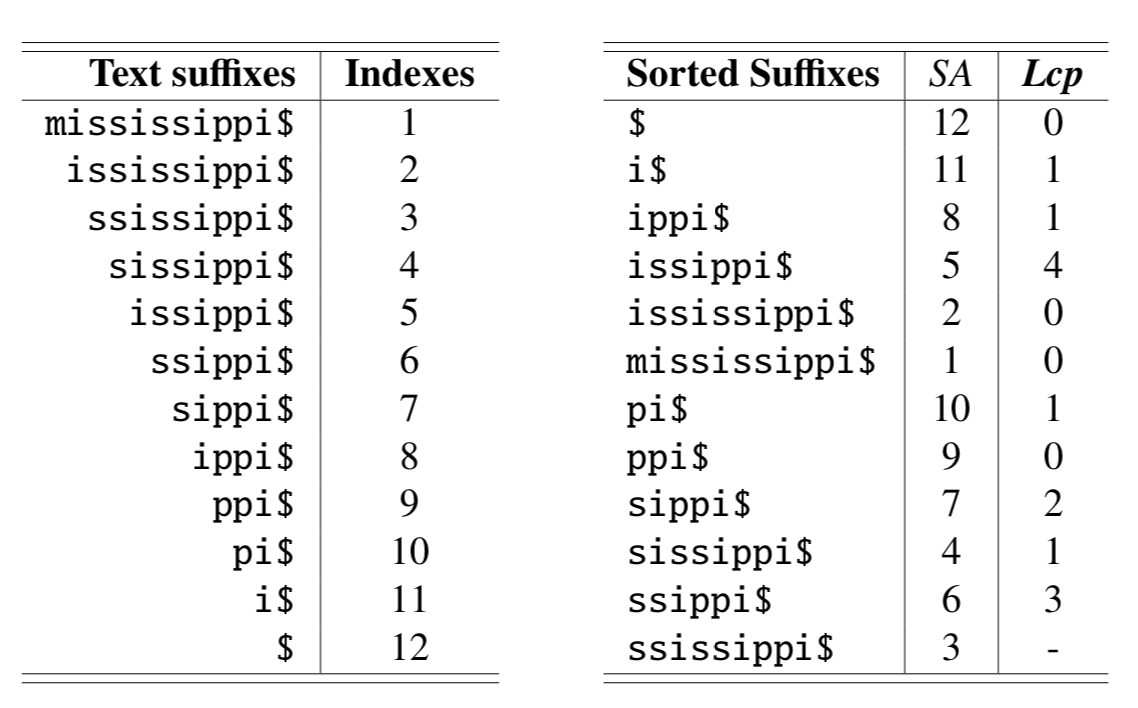
\includegraphics[width=0.7\linewidth]{SUFT.png}
\end{figure}

\section{Suffix Array}

Il suffix array SA è un array di puntatori ai suffissi ordinati di una stringa T. All'interno dell'array ogni suffisso viene identificato con un intero che indica la posizione di partenza del suffisso.
Il suffix array contiene n interi e quindi occupa uno spazio $O(nLogn)$ bit. 
Oltre al suffix array viene mantenuto anche un array LCP che contiene i longest common prefix tra due suffissi consecutivi, all'interno di questo suffix array ci sono $n-1$ interi.

\subsection{Substring Search}

Il problema della ricerca della sottostringa P all'interno della stringa T può essere ridotto alla ricerca di un prefisso P tra l'insieme delle stringhe dei suffissi che si creano nell'array SA(T).
Preso l'array SA viene svolta una ricerca binaria di P all'interno dei suffissi, ad ogni iterazione della ricerca binaria vengono confrontati al più p caratteri. In tutto questa ricecrca binaria mi costa $O(pLogn)$ per capire quante sono le sottostringhe P in T, se poi vogliamo anche trovare quali sono le posizioni ho bisogno di un tempo aggiuntivo che è $O(occ)$. Lo spazio che viene occupato da questa ricerca è $O(nLogn + nLog\sigma)$.
La ricerca binaria è una modifica della ricerca binaria su interi, qua ad ogni iterazione confrontiamo dei caratteri e a seconda di come va il confronto eseguiamo la ricorsione su una parte dell'array o sull'altra.

Abbiamo però la possibilità di migliorare la complessità in tempo di questa procedura andando a considerare che non devo confrontare ogni volta p caratteri perchè in alcuni casi posso saltarne alcuni. Per svolgere questa procedura ho bisogno di alcune informazioni aggiuntive:

\begin{itemize}
\item Abbiamo l'array lcp[1,n-1] in cui salviamo i lcp tra il suffisso i e il suffisso i+1
\item Abbiamo due array di n elementi, ognuno degli elementi dell'array è legato alla tripla $<L,M,R>$ che si crea ad ogni iterazione della ricerca binaria. Dove L è il limite inferiore dell'array, M è il punto medio e R è il superiore. In particolare si va a definire gli array Llcp[] e Rlcp.
$Llcp[M] = lcp(Suff_{SA[M]}, Suff_{SA[L]})$
$Rlcp[M] = lcp(Suff_{SA[M]}, Suff_{SA[R]})$
\item Per ogni iterazione della ricerca binaria salviamo anche due variabili l e r:
$l = lcp(P, Suff_{SA[L]})$
$r= lcp(P, Suff_{SA[R]})$
\item Poi possiamo calcolare LCP(L,R)
\end{itemize}

Ci sono alcune cose che possiamo notare e che ci portano a ridurre il numero di confronti:

\begin{itemize}
\item Il pattern P che ricerchiamo si trova tra L e R quindi condivide con le stringhe che si trovano in questo range almeno LCP(L,R) caratteri.
\item Valgolo le relazioni:
$l\ >\ LCP(L,R)$
$r\ >\ LCP(L,R)$
$Lcp(Suff_{SA[M]},P)\ >\ LCP(L,R)$
\end{itemize} 

Quindi da queste due osservazioni possiamo dire che ad ogni iterazione possiamo scartare i primi $LCP(L,R)$ caratteri e possiamo partire dal successivo durante il confronto del pattern P con $Suff_{SA[M]}$.
C'è un altro dettaglio da considerare, se consideriamo il caso $l \geq r$ abbiamo queste relazioni che ci permettono di escludere altri confronti:

\begin{itemize}
\item Se vale $l \ >\ Llcp[M]$ allora devo eseguire la ricorsione nella prima parte dell'array quindi $m = r$ ma non faccio altri confronti
\item Se vale $l \ <\ Llcp[M]$ allora devo eseguire la ricorsione nella seconda parte dell'array quindi $m = l$ ma non faccio altri confronti
\item Se invece vale $l \ =\ Llcp[M]$ possiamo dire che i primi l caratteri sono in comune tra il pattern P e $Suff_{SA[M]}$ quindi confrontiamo a partire da P[l+1].
\end{itemize}

In questo modo il tempo necessario per l'esecuzione dell'algoritmo passa a $O(p+Logn)$, più $O(occ)$ se vogliamo la posizione delle occorrenze delle sottostringhe. Lo spazio necessario è $O(n)$.


\subsection{Come si crea l'array dei LCP}

L'array LCP con i valori dei longest common prefix è fatto in modo che $lcp[i]=lcp(suff_{SA[i]}, suff_{SA[i+1]})$ e sono presenti al suo interno n-1 interi (dato un SA(T) di n elementi).
La creazione di questo array deve essere fatta in tempo costante, in modo banale potrei farla in $O(n^2)$.
Riducendo il numero di confronti che vengono eseguiti tra i caratteri possiamo arrivare ad un tempo $O(n)$.

Per creare questo array vanno sfruttate due proprietà dell'array dei suffissi.
Una prima proprietà è la seguente:
\newline
\textit{Per ogni x,y con x<y abbiamo che $lcp(Suff_{SA[y-1]}, Suff_{SA[y]})$ è maggiore di $lcp(Suff_{SA[x]}, Suff_{SA[y]})$. Questo vale perchè, dato che i suffissi sono ordinati lessicograficamente, più ci allontiamo da y e più diminuiscono i caratteri in comune all'inizio del suffisso.}

C'è anche una seconda proprietà che vale, a questa possiamo arrivarci se consideriamo i suffissi $suff_{j-1}$ e $suff_{i-1}$ con $suff_{j-1}$ < $suff_{i-1}$ e poi consideriamo  $suff_{j}$ e $suff_{i}$.
tra $suff_{j-1}$ e $suff_{i-1}$ ci sono due probabilità:
\begin{itemize}
\item Non ci sono elementi in comune nel prefix ovvero lcp = 0
\item Ci sono degli elementi in comune ovvero $lcp(suff_{j-1}, suff_{i-1}) > 0$. Sapendo che $suff_{j-1}$ < $suff_{i-1}$ possiamo dire che vale anche $suff_{j}$ < $suff_{i}$ perchè viene preservato l'ordinamento lessicografico e possiamo anche dire che $lcp(suff_{j}, suff_{i}) = lcp(suff_{j-1}, suff_{i-1}) - 1$ perchè dal prefisso originale viene droppato un carattere. 
\end{itemize}

Quindi la seconda osservazione è la seguente:

\textit{Se vale $lcp(Suff_{SA[y-1]}, Suff_{SA[y]})\ >\ 0$ allora possiamo dire che \newline $lcp(Suff_{SA[y-1]+1}, Suff_{SA[y]+1}) = lcp(Suff_{SA[y-1]}, Suff_{SA[y]})\ -\ 1$ }

Vediamo l'implementazione dell'algoritmo, il tempo richiesto è $O(n)$ perchè ci muoviamo sempre verso destra e non facciamo dei confronti in più che non sono necessari:

\begin{code}
\begin{lstlisting}[escapeinside={(*}{*)}]
LCP-Build(char *T, int n, char **SA):
    h = 0
    for (i=0;i<n;i++):
        q = SA^{-1}[i] # prendiamo la posizione di SA[i]
        if q > 1:
            k = SA[q-1]
            if(h > 0):
                h--
            while(T[k+h] == T[i+h]):
                h++
            lcp[q-1] = h
\end{lstlisting}
\end{code}

Esempio di esecuzione dell'algoritmo:

\begin{figure}[H]
\centering
  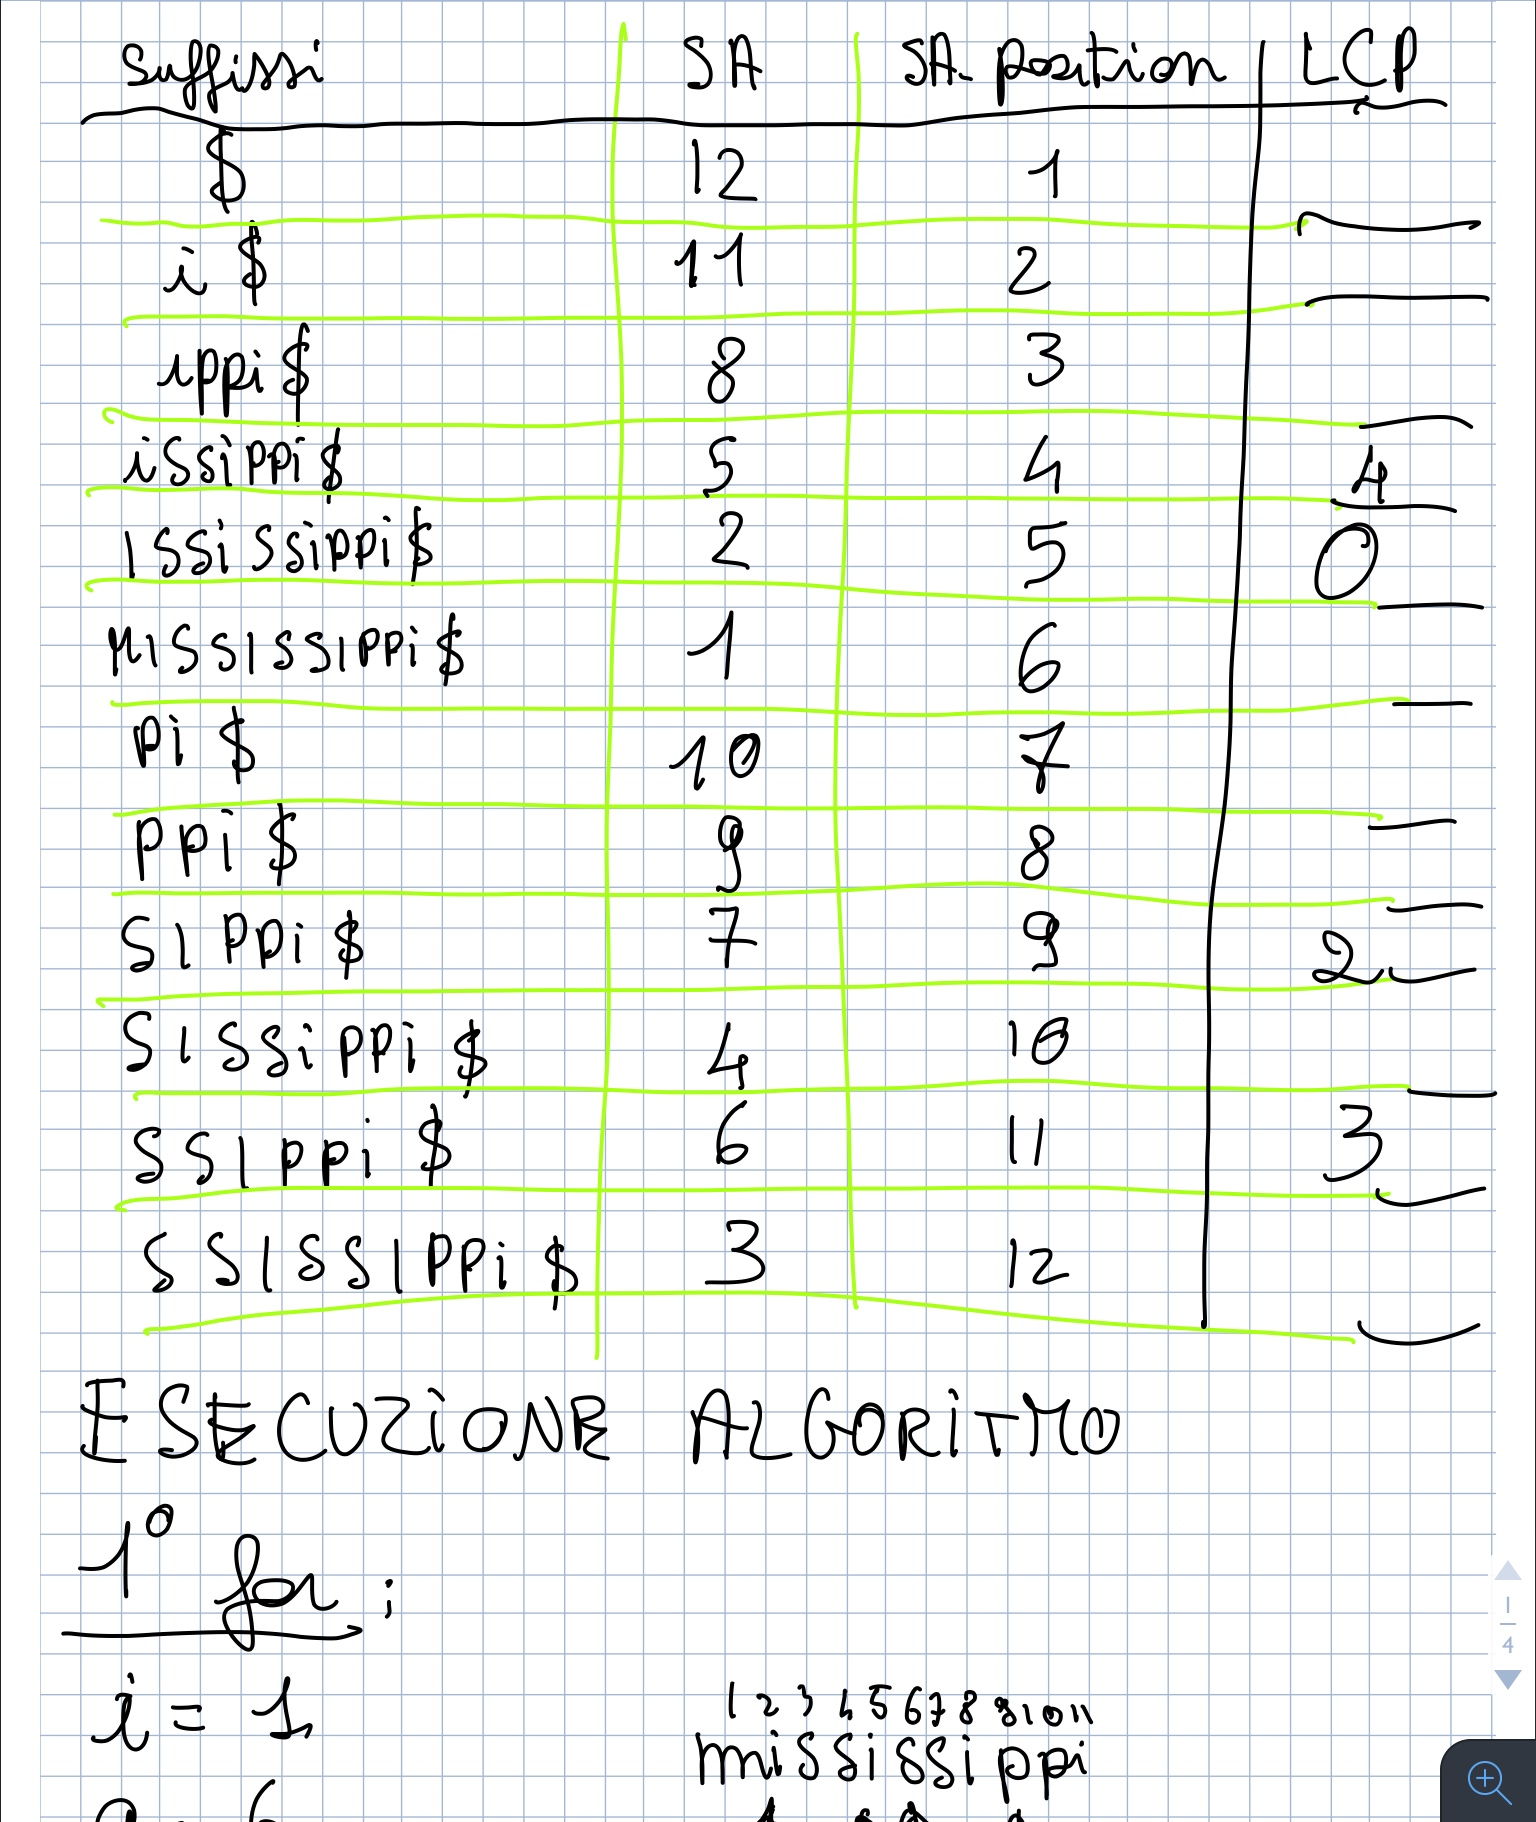
\includegraphics[width=\linewidth]{IMG_0155.jpg}
\end{figure}
\begin{figure}[H]
\centering
  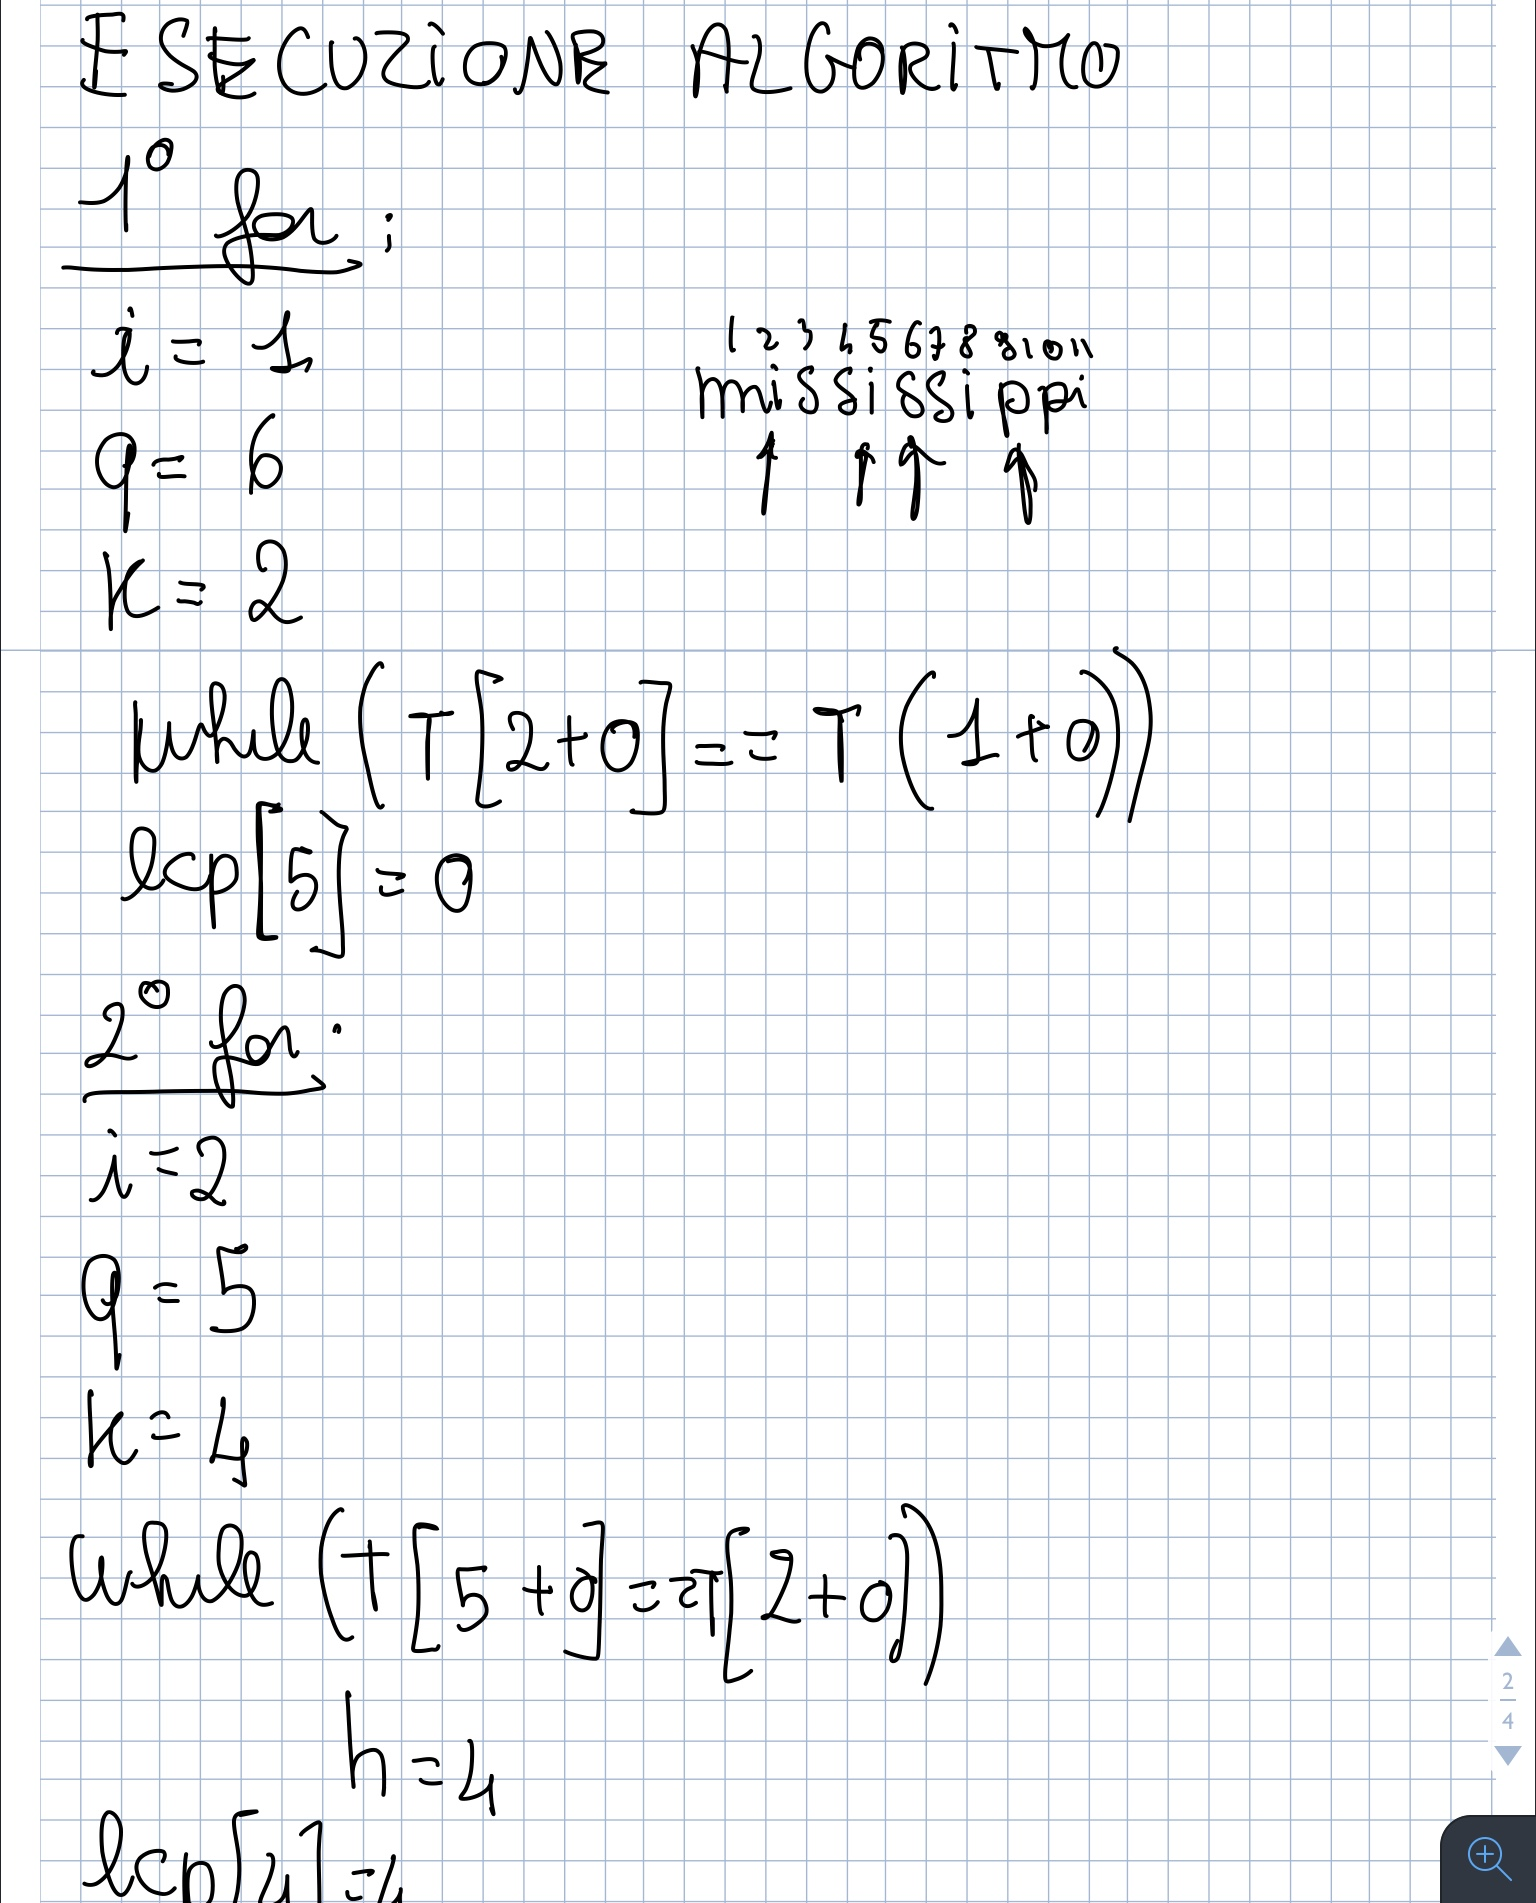
\includegraphics[width=0.6\linewidth]{IMG_0156.jpg}
\end{figure}
\begin{figure}[H]
\centering
  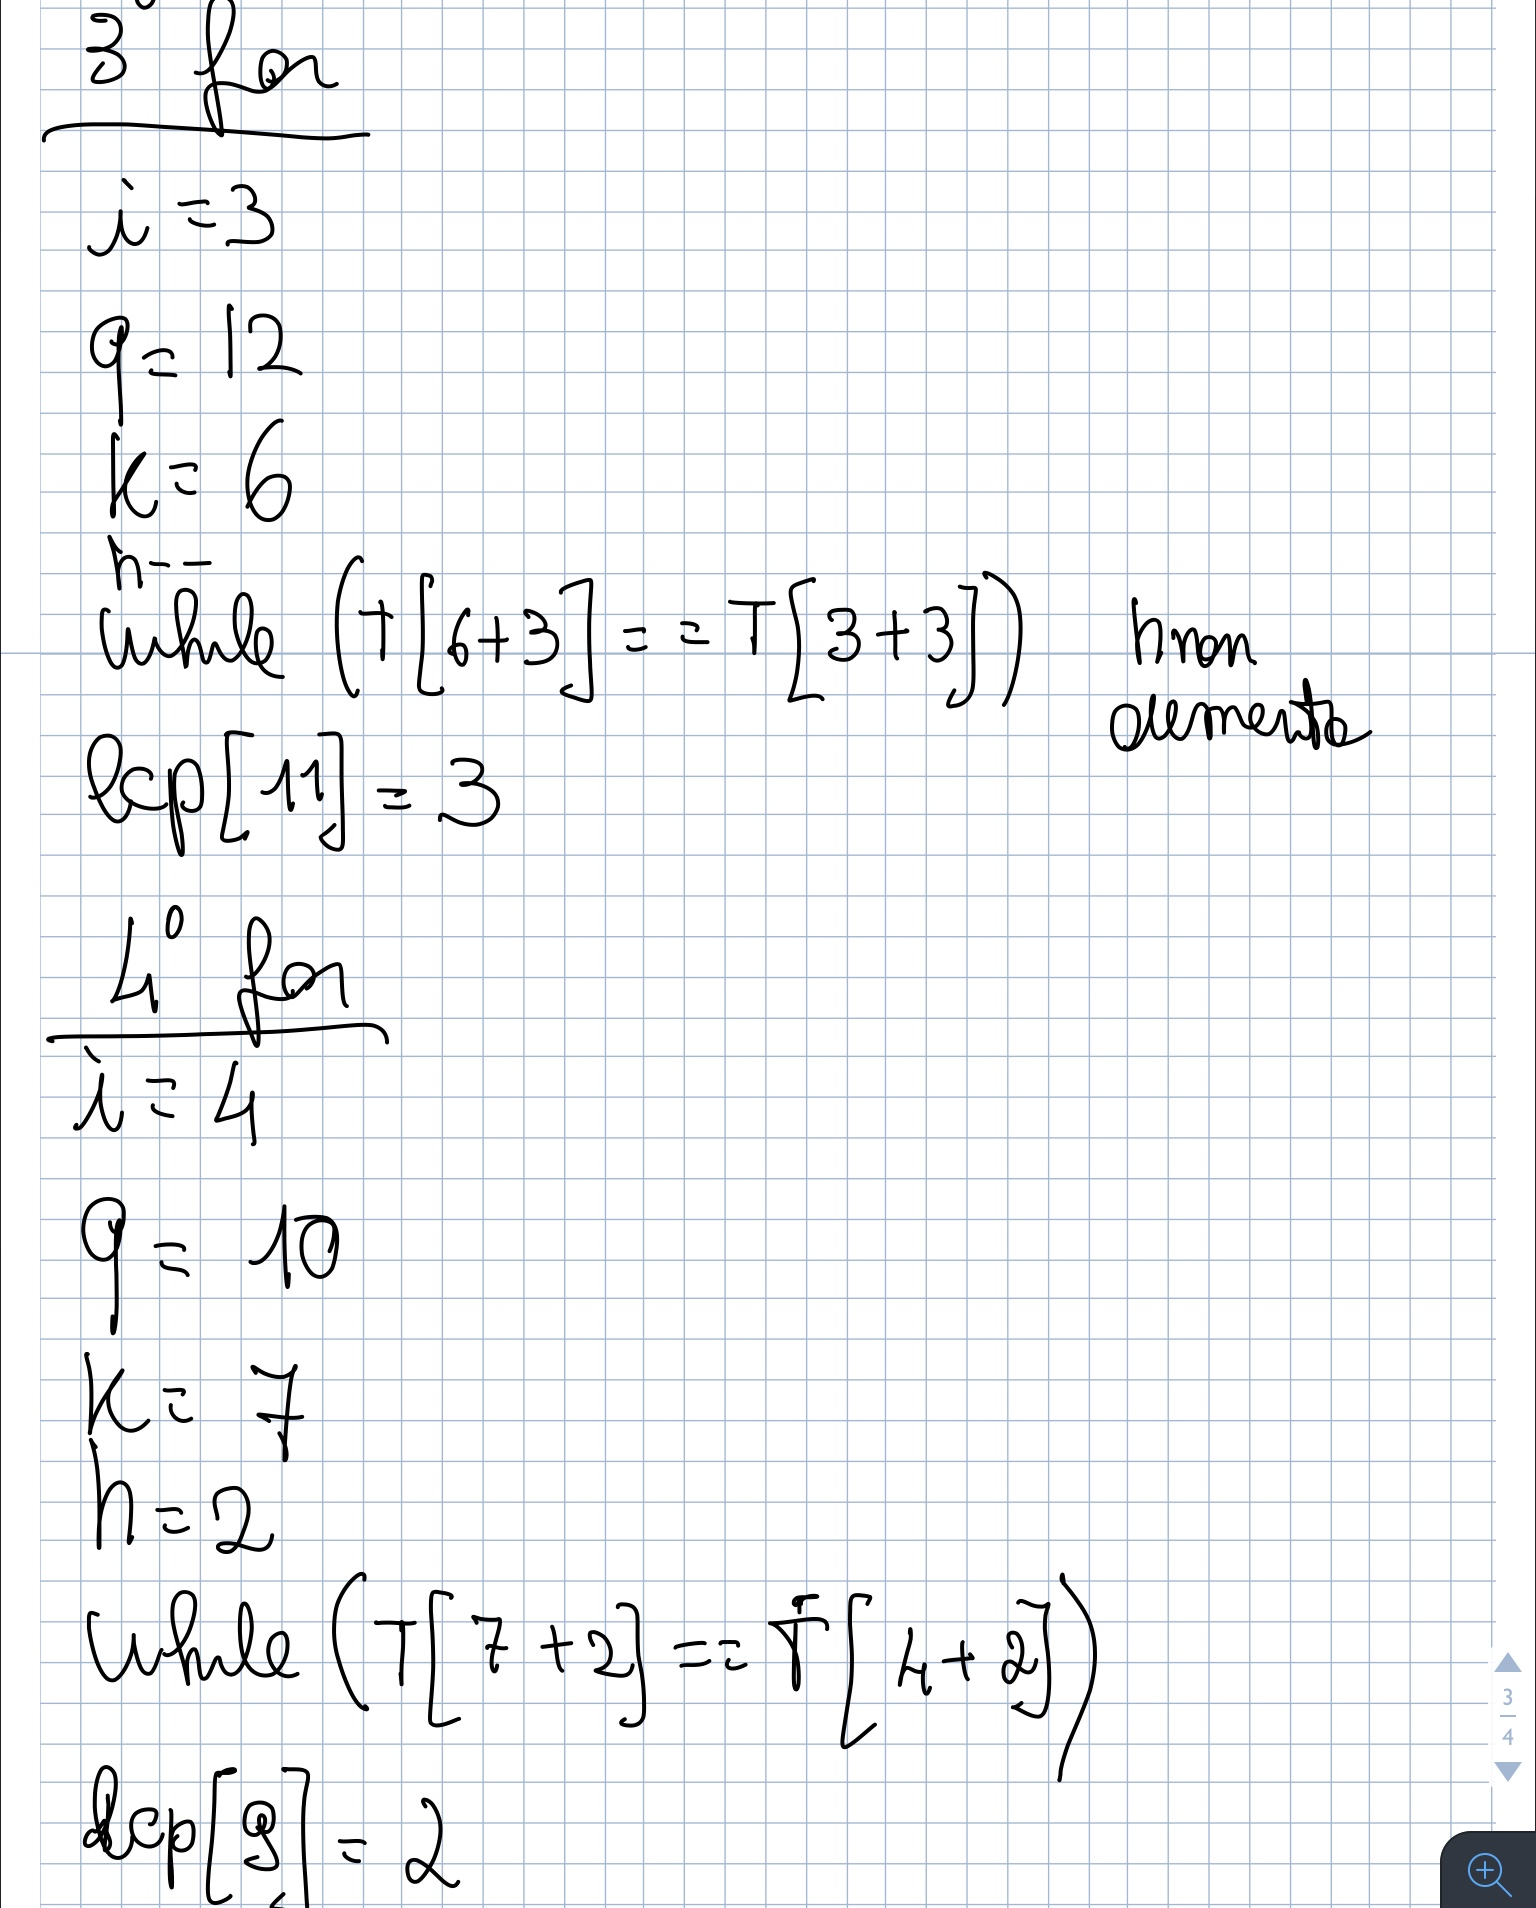
\includegraphics[width=0.6\linewidth]{IMG_0158.jpg}
\end{figure}

\subsection{Costruzione del Suffix Array}

La costruzione del suffix array va svolta utilizzando un algoritmo che mi permetta un ordinamento lessicografico dei suffissi presenti all'interno dell'array SA.
L'idea è di usare un algoritmo tipo il Quick Sort passando come parametro l'algoritmo per il confronto dei suffissi.
L'algoritmo per la creazione dell'SA ordinato crea per prima cosa l'array dei suffissi in cui ogni elemento è un puntatore che punta alla posizione in memoria dei suffissi da ordinare, poi si usa quicksort:

\begin{code}
\begin{lstlisting}[escapeinside={(*}{*)}]
Suffix_cmp(char **p, char **q):
    return strcmp(*p,*q)
\end{lstlisting}
\end{code}
\begin{code}
\begin{lstlisting}[escapeinside={(*}{*)}]
Comparison_based_construction(char *T, int n, char **Sa):
    for(i=0;i<n;i++):
        SA[i] = T+i
    Qsort(SA,n,sizeof(char*), Suffix_cmp)
\end{lstlisting}
\end{code}

Il problema di utilizzare questo algoritmo è che ogni volta che faccio un confronto tra due suffissi (ne faccio $O(nLogn)$), posso confrontare fino a n caratteri, al caso pessimo. Questo si traduce in una complessità al caso pesimo di $O(n^2Logn)$.
Il numero di operazioni I/O che vengono eseguite è $O(\frac{n}{B}nLogn)$, lo spazio necessario è $O(nLogn)$ perchè abbiamo creato l'array SA con n puntatori.


\section{Suffix Tree}

Si tratta di un'altra struttura dati che può essere utilizzata per risolvere il problema del substring search. In questo caso viene utilizzato un compacted trie in cui troviamo n nodi interni che hanno almeno due figli e poi n foglie che rappresentano i vari suffissi.
Quindi in tutto abbiamo $O(n)$ nodi e $O(n)$ archi.
All'interno del Suffix Tree vengono inseriti i vari suffissi della stringa T in cui vogliamo cercare, ogni percorso che va dal nodo root ad una foglia è unico e rappresenta uno dei suffissi.
Tutti gli archi sono associati ad una sottostringa della stringa T, non possiamo memorizzare tutte queste sottostringhe associate agli archi quindi si memorizza la coppia $<start, length>$ che mi dice in che punto inizia la sottostringa e quando finisce.

Notazione:
\begin{itemize}
\item Se abbiamo una sottostringa t tale che la sottostringa che esce dal nodo v è proprio v, ovvero $t==s[v]$ allora quel nodo v è detto locus
\item Se invece abbiamo una stringa t che finisce nel mezzo di un arco (u,v) allora il nodo v è detto extended locus di t.
\end{itemize}

Valgono quindi delle regole:

\begin{itemize}
\item Data una sottostringa $\alpha$, se esiste un nodo interno u tale che $s[u]==\alpha$ allora il nodo u è locus e ci sono due occorrenze di $\alpha$ in T che sono seguite da due lettere diverse
\item Se invece abbiamo una sottostringa $\alpha$ di T che ha un extended locus, allora il carattere successivo della sottostringa $\alpha$ in T sarà sempre uguale.
\item Ogni nodo interno u ha un arco uscente segnato come $s[u]$ che indica la sottostringa massima tra i nodi che stanno sotto di lui e che non può essere esteso di alcun carattere.
\end{itemize}

Come trovo l'lcp tra due suffissi? Dati i suffissi $T[i,n]$ e $T[j,n]$, l'lcp di questi due è il longest common ancestor (lca) ovvero il nodo più profondo che è antenato di entrambi i nodi.

\subsection{Come risolvere il substring search}

Il problema del substring search viene risolto tramite il suffix tree andando a fare una ricerca della sottostringa che cerchiamo a partire dal nodo root, andiamo avanti nel nostro percorso verso le foglie fino a quando non troviamo un mismatch tra il carattere nel percorso e il carattere nella sottostringa che cerchiamo.
Quando troviamo un percorso che matcha completamente la sottostringa che stiamo cercando, possiamo dire che tutti i nodi presenti sotto a quel percorso hanno come prefisso la sottostringa cercata. Quindi se abbiamo occ nodi, possiamo trovare la posizione di queste occ sottostringhe in $O(occ)$.

Il costo della ricerca di un pattern P di lunghezza p all'interno del suffix tree è in tempo $O(p+occ)$ se utilizziamo una hash table perfetta per mantenere salvati i figli dei nodi del nostro albero.

\subsection{Passare da SA a ST e da ST a SA}

\subsubsection{Passare da ST a SA}

Il passaggio da ST a SA è facile e viene fatto in $O(n)$ perchè viene fatta una visita in-order del suffix tree e ogni volta che troviamo una foglia, il puntatore corrispondente viene scritto nell'array SA, quando trovo il nodo interno associamo quel valore all'array lcp.


\subsubsection{Passare da SA a ST}

Anche il passaggio da SA a ST viene svolto in $O(n)$ però è un po' più complesso:
\begin{itemize}
\item La costruzione avviene in modo incrementale e ad ogni passaggio sappiamo che è stato costruito il suffix tree parziale $ST_{t-1}$.
\item Al primo passaggio abbiamo nel suffix tree il nodo root che ha valore 0 e poi abbiamo $SA[1]$.
\item Nei passaggi successivi andiamo ad inserire gli elementi successivi dell'array, l'inserimento viene effettuato partendo dall'ultimo elemento che ho inserito all'interno dell'albero, da questo eseguiamo una visita verso l'alto dell'albero e ci fermiamo quando troviamo un nodo x tale che $lcp[i-1]\ \leq \ |s[x]|$.
\item In pratica quando inserisco un nodo vedo se nel percorso dall'ultimo nodo inserito al root ho già un elemento che ha il valore di $lcp[l-1]$, se c'è aggiungo il nuovo nodo come figlio di questo nodo, altrimenti devo creare un nuovo branching node con valore $lcp[l-1]$ che ha come figli l'ultimo nodo inserito e quello che devo inserire in questo passaggio.
\end{itemize}

\subsection{Text Mining}

Ci sono alcuni problemi di text mining che possono essere risolti facilmente utilizzando i SA con l'array lcp o i ST.

\begin{itemize}
\item Se prendiamo due suffissi dell'array SA, ad esempio i e j, e vogliamo capire il loro lcp dobbiamo considerare l'array lcp e prendere il minimo valore che è compreso nel range lcp[i,j].
Quindi abbiamo $lcp(SA[i], SA[j])\ =\ min(lcp[i,...,j])$.
\item Cerchiamo se esiste la sottostringa che si ripete almeno C volte. Possiamo risolvere questo problema con il ST andando a vedere se c'è un nodo che ha almeno C foglie sotto. Se vogliamo risolverlo con il SA dobbiamo vedere se c'è un sub array di SA di lunghezza almeno C che ha un lcp associato maggiore di 0.
\item Se cerchiamo se esiste una sottostringa di lunghezza maggiore di L che si ripete almeno C volte.
È una variante del problema precedente, in questo caso se vogliamo usare l'albero dobbiamo vedere sia se c'è un nodo u che ha almeno C foglie e sia se $|s[u]|>L$. Lo stesso vale per l'array, dobbiamo cercare il subarray che è lungo almeno C elementi e che ha associati valori dell'lcp array $\geq \ L$.
\item Se vogliamo vedere se c'è una sottostringa che si ripete più di due volte ed è lunga almeno L.
Nel caso del ST, ammesso che esiste una sottostringa che si ripete più di due volte, devo prendere le due foglie che corrispondono ai suffissi $suff_i$ e $suff_j$ e poi devo andare a calcolare il longest common ancestor lca(i,j) che mi restituisce un certo nodo x, se il nodo x ha una $|s[x]|>L$ allora vuol dire che esiste questa sottostringa.
Se lo stesso problema lo vogliamo risolvere con il SA devo considerare che le sottostringhe che si ripetono più di una volta sono una vicina all'altra nel SA quindi l'array LCP associati a questi due valori deve avere valore L.
\end{itemize}


\section{Approximate Pattern Matching}

Si tratta del problema di cercare un pattern P di lunghezza p all'interno di un testo T di lunghezza n, vengono considerate valide le sossostringhe di T che hanno un match parziale con P con un numero di mismatch che al più è pari a k.
Il problema in questione ha applicazioni anche in bio-informatica.
Una soluzione banale che costa $O(pn)$ consiste nel prendere le varie sottostringhe di T e andare a vedere se il numero di match tra la sottostringha e il pattern è minore di k.
Una soluzione migliore utilizza anche una struttura dati utilizzata anche per il problema del Range Minimum Query.
L'algoritmo che viene utilizzato per questo problema alla fine costa in tempo $O(nk)$ perchè funziona in questo modo:
\begin{itemize}
\item Se abbiamo la stringa T e il pattern P, possiamo allineare le due stringhe e vedere che avremo un numero j di sottostringhe che coincidono e un numero j di caratteri che segnano il mismatch.
\item Se il numero di mismatch è minore di k allora possiamo dire che quel pattern è presente all'interno della stringa T.
\item Se ad esempio troviamo che $T[i,i+l]=P[j,j+l]$ per poi avere un carattere di mismatch, possiamo dire che attualmente il lcp tra la sottostringa di T e P è l ma possiamo andare avanti con una seconda iterazione in cui andremo a calcolare l'lcp tra $T[i+l+1]\ e\ P[j+l+1]$.
Il numero di iterazioni che svolgo è pari al numero k di mismatch che voglio ci siano nel confronto tra il pattern e la stringa T.
\end{itemize}

La complessità in tempo è $O(nk)$ ma questo è vero se troviamo un modo per eseguire il calcolo dell'lcp in $O(1)$.
Questo calcolo è possibile utilizzando i dati relativi all'lcp che mi salvo nel SA o anche nel ST però dobbiamo creare in modo differente i nostri suffissi perchè dobbiamo unire la stringa T con il pattern per ottenere una stringa $X=T#P$.
In questo modo il calcolo dell'lcp tra il pattern e la stringa diventa il calcolo dell'lcp tra due sottostringhe della stringa X.

L'algoritmo che viene utilizzato il pattern matching approssimato:

\begin{code}
\begin{lstlisting}[escapeinside={(*}{*)}]
matches = {}
for i=1 to n:
    m = 0, j = 1;
    while (m<k) and (j<p):
        l = lcp(T[i+j-1,n],P[j,p])
        j = j+l
        if (j<p):
            m = m+1
            j = j+1
    if m<k:
            matches = matches + T[i,i+p-1]
\end{lstlisting}
\end{code}

\subsubsection{Legame tra lcp e lca}

Ricordiamo che noi dobbiamo trovare un modo per risolvere il problema dell'lcp in $O(1)$.
Prendiamo una certa stringa T e creiamo il suo suffix tree. Consideriamo due suffissi, $X[i,x]$ e $X[j,x]$, tra questi due c'è un prefisso in comune che viene indicato dal nodo u che è antenato di entrambi. C'è quindi un legame tra il problema dell'lcp e quello dell'lca (longest common anchestor). In particolare il nodo u antenato di entrambi i suffissi avrà un $|S[u]|$ associato che rappresenta la lunghezza dell'lcp delle due sottostringhe.
Lo stesso problema può essere risolto anche utilizzando il suffix array e il relativo array con i vari lcp. In particolare prese le sottostringhe $X[i,x]$ e $X[j,x]$ per cui vogliamo calcolare l'lcp, devo andare a prendere le corrispondenti posizioni nell'array lcp e poi prendere il minimo dei valori compresi tra queste due posizioni.
Questo valore minimo è esattamente $|S[u]|$ che abbiamo nominato prima ed è la lunghezza del longest common prefix.
Questa seconda soluzione che consiste nel trovare il minimo in un range all'interno di un array prende il nome di Range Minimum Query problem (RMQ).
Il problema, dato un array A[1,n] consiste nel trovare il minimo elemento all'interno del range (i,j) in modo da restituire la posizione di questo valore minimo.

Una soluzione banale al problema consiste nel prendere tutte le possibili coppie i,j e calcolare il minimo compreso in quel range, poi si mettono tutti i risultati in una hash table in tempo $O(n^2)$ e spazio $O(n^2)$.

Un'altra soluzione è il metodo sparsification, in questo caso partiamo da un indice i e andiamo a calcolare ad ogni iterazione il minimo del range $(i,i+2^L-1)$ dove $L=Log(j-i+1)$. In questo modo l'array in cui salviamo i minimi mi occupa $O(nLogn)$.
Se voglio risolvere il problema dell'RMQ di un certo range:
$RMQ(i,j)=argmin(RMQ_a(i,i+2^L-1),RMQ(j-2^L+1,j))$ eseguo questa query e ottengo la risposta in $O(1)$.

Possiamo utilizzare il metodo sparsification con una variante andando a dividere in blocchi l'array A di partenza:
\begin{itemize}
\item Dividiamo A in $n/b$ blocchi e ogni blocco ha $Logn$ elementi.
\item Per ognuno dei blocchi calcoliamo il minimo e lo salviamo in un array A' che quindi occuperò $O(\frac{n}{Logn})$.
\item Poi usiamo il metodo sparsification sull'array A' e quindi in questo modo abbiamo $RMQ_A$ che mi occupa $(O(|A'|Log|A'|)) = O(n)$.
\end{itemize}

Ora se vogliamo risolvere le query RMQ:
\begin{itemize}
\item Se abbiamo la richiesta di RMQ che combacia direttamente con un blocco dell'array ottengo la risposta in O(1)
\item Se abbiamo una query in cui i due limiti escono fuori da un blocco e quindi coprono un blocco per intero e due in parte dobbiamo andare a calcolare il minimo di due sottoblocchi $B_i[i,b]$ e $B_j[1,i]$. Per farlo possiamo salvarci per ogni blocco i minimi dei vari sottoblocchi con uno spreco di spazio pari a $O(b*\frac{n}{b})=O(n)$.
Anche in questo caso si risolve il problema in $O(1)$.
\end{itemize}

Il problema si presenta quando dobbiamo calcolare RMQ di un sottoblocco. 
Per risolverlo vengono fatte due riduzioni:
\begin{itemize}
\item La prima riduzione è dal problema RMQ al problema LCA
\item La seconda riduzione è dal problema LCA a RMQ
\end{itemize}

Per quanto riguarda la prima riduzione, si parte con un array di interi (che sarebbe il nostro array lcp) e poi andiamo a creare un cartesian tree. Il cartesian tree lo costruisco così:
\begin{itemize}
\item Prendiamo il minimo dell'array e questo diventa il nodo root nel formato $<valore minimo, posizione>$. Dove posizione = m.
\item Il cartesian tree ha due figli, è binario. Il figlio sinistro sarà il minimo che troviamo nel sub array che va da 1 a m e il sub array a destra sarà il minimo del sub array che va da m a n dove n è la lunghezza complessiva dell'array.
\item Ricorsivamente andiamo avanti in questo modo costruendo l'albero.
\end{itemize}

Se vogliamo calcolare il RMQ(i,j) ovvero il minimo del range (i,j), il problema può essere affrontato usando il cartesian tree andando a risolvere lca(i,j) ovvero trovando il common anchestor di i e di j all'interno del cartesian tree.

\textbf{Poi va fatta una seconda riduzione da LCA e RMQ.}

Per la seconda riduzione trasformiamo il problema dell'LCA da svolgere sul cartesian tree in un RMQ da svolgere su un array binario.
\begin{itemize}
\item Partiamo dal Cartesian tree creato al passo precedente, svolgiamo un euler tour di questo albero andando ad inserire in un array $\Delta[1,2e]$ (dove e è il numero di archi visitati) il valore dei vari nodi che visitiamo.
\item Mentre creiamo l'array dell'euler tour creiamo anche un secondo array D in cui inseriamo la profondità del nodo che stiamo visitando.
La particolarità di questo array D è che c'è una differenza di 1 tra i vari elementi che sono presenti al suo interno. Ogni interò è +1 o -1 rispetto al precedente.
\end{itemize}

Ora vogliamo risolvere il problema del LCA, se prendiamo il CT, e dobbiamo trovare il LCA(i,j) tra due nodi i e j possiamo utilizzare l'array D e svolgere RMQ(pos(i), pos(j)) dove con pos indichiamo la posizione di i e j che viene trovata prendendo la i più a sinistra nell'array dell'euler tour e la j più a destra.

Il problema RMQ può essere risolto sull'array D in spazio $O(n)$ e tempo $O(1)$:

\begin{itemize}
\item L'array D viene diviso in blocchi di dimensione $d=\frac{1}{2}Log e$, ogni blocco $D_k$ è formato da $\frac{2e}{d}$ elementi.
\item Per ogni blocco $D_k$ calcoliamo il minimo che viene salvato in un array A che avrà al suo interno un numero di elementi pari al numero di blocchi. 
\item Applichiamo il metodo sparsify sull'array appena creato creando un secondo array M che avrà dimensione $|A|\ Log\ |A|$ ovvero $\frac{e}{Loge}Log \frac{e}{Loge}\ =\ O(n)$.
\end{itemize}

Ci serve una seconda struttura dati per coprire anche il caso in cui le i,j di RMQ(i,j) sono interne ad un blocco.
\begin{itemize}
\item L'array D viene trasformato, ogni blocco $D_k$ viene scritto nella forma $<D_k[1], \Delta_k>$ Dove in $\Delta_k$ ogni elemento è 1 o 0, 1 se nell'array D abbiamo un +1 rispetto all'elemento precedente e 0 se abbiamo un -1.
\item Per ogni blocco salviamo anche la coppia $\Delta_k, posizione minimo$.
\end{itemize}

Notiamo che abbiamo $2^{d-1}$ possibili $\Delta_k$, li vogliamo elencare tutti quanti e per ognuno elencare la possibile posizione del minimo, in tutto sono $2^{\frac{Loge}{2}} = O(\sqrt{n})$.
In più vogliamo considerare tutte le possibili coppie (i,j) prese all'interno di $D_k$, abbiamo $d=\frac{1}{2}Log e$ possibili valori per ognuno dei due quindi in tutto abbiamo $O(Log^2 e) = O(Log^2 n)$ possibili coppie.
Vogliamo creare una tabella T in cui troviamo $<i_0,j_0, \Delta_k, pos min>$, questa tabella avrà un numero di entry pari a $O(\sqrt{n})*O(Log^2 n)$ ovvero $O(n)$ entry e lo creiamo in $O(n)$.

Ora, se dobbiamo risolvere la query RMQ(i,j) con i,j che sono interni al blocco $D_k$, dobbiamo fare due passaggi:
\begin{itemize}
\item Prima calcoliamo $i_0$ e $j_0$ che sono le nuove posizioni di i e di j all'interno di $D_k$. Prendiamo la corrispondente configurazione $\Delta_k$.
\item Usiamo la tripla $<i_0,j_0,\Delta_k>$ per andare ad accedere alla tabella T in tempo $O(1)$.
\end{itemize}


Quindi per eseguire il calcolo dell'RMQ in un array A, possiamo utilizzare una struttura dati che ci permette di risolvere il problema in $O(1)$. La risoluzione di questo problema in $O(1)$ ci permette di risolvere anche il LCA in $O(1)$.

\chapter{Codifica degli interi}

Il problema di codificare un insieme di interi consiste nell'avere un array di interi positivi S = [$s_1,...,s_n$] e volerli rapresentare come una sequenza binaria che utilizza un numero minore di bit.
Gli interi devono essere positivi, se sono negativi possiamo apportare una trasformazione ovvero, quelli già positivi diventano $x\ ->\ 2x$, quelli negativi invece diventano $x\ ->\ -2x+1$.

Se abbiamo questa sequenza di interi una prima idea potrebbe essere quella di andare a prendere l'intero m più grande e utilizzare quindi $logm\ +\ 1$ bit per rappresentare tutti gli interi della sequenza.
Questo metodo sicuramente funziona ed è anche veloce decodificare la sequenza codificata, il problema è che abbiamo uno spreco di spazio perchè se c'è una grande distanza tra gli interi più piccoli e m allora vuol dire che utilizziamo logm + 1 bit per rappresentare interi che potrebbero essere rappresentati con molto meno.

Un'alternativa consiste nell'utilizzo di un numero variabile di bit, quindi per ogni intero $s_i$ vengono utilizzati $1+log\ s_i$ bit. In questo caso il problema però sta nel delimitate i vari blocchi di bit perchè leggendo la sequenza codificata potremmo avere varie interpretazioni.

Un'altra alternativa consiste nell'utilizzare lo unary coding, in questo caso preso l'intero $x$, utilizziamo un numero x-1 di 0 seguito da un solo 1 per rappresentare l'intero. In questo modo abbiamo bisogno di x bit per rappresentare l'intero. Si spreca tempo e se gli interi sono grandi non è molto efficiente.

Per parlare di efficienza dei vari sistemi per il coding di sequenze di interi si deve considerare in particolare il teorema di Shannon secondo cui: \newline
\textit{Dato un simbolo c da codificare, la lunghezza ideale L(c) della sua codifica è uguale a $Log_2\frac{1}{Pr[c]}$} dove Pr[c] è la probabilità che compaia il simbolo c che dobbiamo codificare.
Questo teorema lo possiamo utilizzare per uguagliare il valore indicato da Shannon al numero di bit necessario per codificare un certo intero in modo da capire la distribuzione di probabilità ideale per poter utilizzare quel certo tipo di coding.

Sempre parlando di performance possiamo parlare del costo medio di un encoder:
\begin{equation}
\sum_x p(x)*|len(x)| \geq \sum_x p(x)*Log \frac{1}{p(x)}
\end{equation}

In particolare $\sum_x p(x)*Log \frac{1}{p(x)}$ indica l'entropia della sequenza di interi da codificare, se fissiamo $p(x)=\frac{1}{|s|}$, il valore di H oscilla tra 0 e $log_2|S|$, se è vicino a 0 allora abbiamo una serie di interi che sono molto compressi, se invece abbiamo un valore molto vicino a $log_2|S|$ allora la distribuzione degli interi è random.


Possiamo utilizzare lo shannon Theorem per capire la distribuzione ottimale che devono avere gli interi quando utilizziamo lo unary encoding o il Fixed Length Binary Code:

\begin{itemize}
\item Fixed Length Binary Code: ogni intero viene codificato con $1+logm$ bit quindi abbiamo 
\begin{equation}
Log_2\frac{1}{Pr(x)} = 1+log m 
\end{equation}
Ovvero Pr(x) = $\frac{1}{m}$.
\item Nello Unary Encoding invece (per togliere log eleviamo alla seconda x e il primo termine):
\begin{equation}
Log_2\frac{1}{Pr(x)} = x\ quindi \ \frac{1}{Pr(x)} = 2^x
\end{equation}
Quindi Pr(x) = $2^{-x}$.
\end{itemize}


\section{Gamma Code: $\gamma$}

Il Gamma code è uno universal code perchè la lunghezza della sequenza codificata è $O(Logx)$ quindi lontano solamente per una costante rispetto all'ottimo.

Il Gamma Code funziona in questo modo:
\begin{itemize}
\item Dato X da codificare, codifichiamo X in binario B(X)
\item Prendiamo la lunghezza della codifica in binario e la rappresentiamo con la rappresentazione unaria $U(|B(X)|)$.
\item Alla fine la codifica del nostro intero sarà $U(|B(X)|)$ seguita da $B(X)$.
\end{itemize}

Per questa rappresentazione, la lunghezza di $B(X)$ è $Logx+1$, per la rappresentazione unaria abbiamo $Logx$. Quindi in tutto abbiamo $2Logx\ +\ 1$.
Secondo il teorema di Shannon dobbiamo uguagliare $Log_2\frac{1}{Pr[X]}=2Logx\ +\ 1$.
Questo ci dice che la distribuzione di probabilità che deve avere la sequenza per usare il Gamma code è: $\frac{1}{2x^2}$

Il Gamma code è lento per la decodifica.

\section{Delta Code: $\delta$}

Nel caso del delta code abbiamo una situazione simile alla precedente, preso X da codificare abbiamo:

\begin{itemize}
\item Codifichiamo X in binario creando $B(X)$ che richiede uno spazio $LogX+1$
\item Prendiamo la lunghezza di $B(X)$ e la codifichiamo con il Gamma code, creando quindi una rappresentazione in binario e una unaria. Questa mi costa $Log(|B(X)|)+1$ per la rappresentazione in binario e in più $Log(|B(X)|)$ per la rappresentazione unaria. Quindi in tutto abbiamo $2Log(|B(X)|)\ +\ 1$.
\item Nel complesso abbiamo $2Log(LogX)\ +\ 1\ +\ LogX$ bit per rappresentare un intero con il delta code.
\end{itemize}

Quindi usando il teorema di Shannon possiamo fare l'uguaglianza e dire che la distribuzione per cui è ottimo è $\frac{1}{2x(Logx)^2}$.

Il Delta code è molto lento per la decodifica.

\section{Rice Code}

L'encoding di Rice dipende da un parametro k che viene scelto dall'utilizzatore, viene utilizzato quando abbiamo degli interi che sono tutti intorno ad un certo valore.
Dato l'intero X da codificare e il parametro k, la codifica funziona in questo modo:

\begin{itemize}
\item Calcoliamo quoziente $q=\frac{x-1}{2^k}$ e resto $r=x-2^k*q-1$
\item Ora q viene rappresentato con la rappresentazione unaria mentre r viene rappresentato in binario.
\item La rappresentazione in binario mi prende k bit perchè rappresentiamo gli interi compresi tra $[0,2^k]$. La rappresentazione unaria mi prende q+1 bit. Nel complesso abbiamo una lunghezza dell'intero codificato pari a $k+q+1$.
\end{itemize} 

Per la decodifica, la prima parte viene letta di bit in bit mentre la seconda viene letta in un solo colpo perchè conosciamo il valore di k.
La distribuzione ottima per il Rice code è $(1-p)^{x-1}p$ che è una distribuzione geometrica dove la p è pari a $0.69*Average(s)$.

\section{PForDelta Code}

L'encoding con PForDelta viene utilizzato quando abbiamo una distribuzione gaussiana dei dati del nostro array.
Assumiamo che la maggior parte dei valori del nostro array sono nell'intervallo $[base, base+2^b-1]$, questi vengono proiettati nell'intervallo $[0, 2^b-1]$ andando a sottrarre il valore di base.
L'idea è di andare a rappresentare questi valori con b bit compresi nell'intervallo $[0, 2^b-1]$ mentre gli interi per cui non bastano b bit vengono inseriti in un array di eccezioni e nel primo array viene inserito un carattere escape che può corrispondere all'ultimo valore rappresentabile con b bit ovvero $2^b-1$.
Quando utilizziamo PForDelta quindi partiamo da un certo array, prendiamo come base il primo elemento dell'array e andiamo a sottrarre a tutti quell'elemento. Poi eseguiamo una compressione con gap encoding e poi eseguiamo PForDelta.
Alla fine ogni intero viene codificato con b bit oppure con $b+w$ bit.

È fondamentale scegliere bene b perchè se prendo un valore troppo piccolo ho un array di eccezioni molto grande, se invece lo prendo troppo grande allora ho uno spreco di memoria perchè abbiamo che gli interi più piccoli vengono rappresentati con b bit quando gliene basterebbero molti di meno.
L'idea è di scegliere una b che ci permetta di avere il 90\% degli interi della sequenza all'interno dell'intervallo $[0,2^b-1]$.
Esistono anche dei metodi basati su programmazione dinamica che ci permettono di scegliere la b che andrà a minimizzare il numero di interi che poi finiranno all'interno dell'array delle eccezioni.
Un'altra possibile soluzione (\textbf{poco chiara}) consiste nel flippare la gaussiana, si ha quindi un nuovo "divisore" della gaussiana che sta al centro e che va a dividere gli interi in positivi e negativi, gli interi vengono poi resi tutti positivi moltiplicando i positivi per $2x$ e i negativi per $-2x+1$, poi una volta fatta questa modifica si va ad applicare l'algoritmo PForDelta scegliendo la b.


\section{Variable Byte Code}

Questo metodo viene utilizzato se la sequenza che vogliamo codificare contiene dei numeri molto grandi.
Preso un certo X da codificare, lo scriviamo in binario, dividiamo la rappresentazione in binario in blocchi di 7 bit, se la lunghezza complessiva non è multipla di 7 dobbiamo inserire degli 0 all'inizio della sequenza.
Davanti a tutti i blocchi di 7 bit deve essere aggiunto un altro bit, questo sarà 0 per l'ultimo di questi blocchi mentre sarà 1 per tutti gli altri.
Tutto questo ci porta ad avere una codifica che occupa $\frac{B(X)}{7}$ bytes ovvero $8*\frac{B(X)}{7}$.
L'encoding con Variable Byte è ottimo se abbiamo la distribuzione $Pr[X] = \sqrt[7]{\frac{1}{x^8}}$.

Per quanto riguarda la decodifica, viene letto 1 byte alla volta fino a che non trovo un byte che ha un valore minore di 128. In quel momento vuol dire che sono arrivato all'ultimo blocco che deve essere letto.
I blocchi che hanno un 1 davanti sono detti continuers mentre quelli che hanno lo 0 sono detti stoppers.
Le possibili configurazioni di continuers e stoppers sono 128, in tutto quindi, facendo la somma sono $2^b=2^8=256$.


\section{S,C Code}

Possiamo notare che con alcuni tipi di distribuzione degli interi della sequenza potremmo avere una migliore codifica (risparmiando spazio) se utilizzassimo una differente quantità di configurazioni per stopper e continuer.
L'importante è che la somma delle configurazioni degli stopper e dei continuer sia sempre pari a $2^b$ dove b è la dimensione dei vari blocchi.
In particolare se abbiamo una sequenza di numeri che sono molto piccoli, ci conviene utilizzare una quantità più grande di configurazioni per gli stopper mentre una minore per i continuer.
Se invece abbiamo una distribuzione meno concentrata in alcuni punti, sarà meglio avere una scelta più distribuita delle varie configurazioni. 
Esempio:\\
Prendiamo $b=3$:
\begin{itemize}
\item Se fissiamo $s=4$ e $c=4$ dove con $s$ e $c$ indichiamo il numero di configurazioni di stopper e continuer, stiamo dicendo che soltanto 4 configurazioni saranno riservate per gli stopper, quindi i numeri dopo il 3 dovranno essere rappresentati con almeno un continuer e uno stopper.
\item Se fissiamo $s=6$ e $c=2$ abbiamo invece che i numeri fino a 5 sono codificati come stopper. Se la distribuzione degli interi da codificare è concentrata tra i primi numeri, questa è l'assegnamento di configurazioni da preferire.
\end{itemize}

\section{Interpolative Code}

Si tratta di un encoding che sfrutta l'ordinamento della sequenza di interi che vogliamo codificare, inoltre viene utilizzato soprattutto se all'interno della sequenza abbiamo dei cluster di interi ovvero se ci sono dei sub array in cui compaiono degli interi concentrati in range piccoli.
L'encoding in questione è ricorsivo e ogni intero che viene codificato non dipende solamente dall'intero stesso ma anche da altri elementi della sequenza.

Ad ogni iterazione mi servono i seguenti dati:

\begin{itemize}
\item L'indice l che è il più a sinistra nell'array e l'indice r che è il più a destra
\item la lunghezza n dell'array
\item l'elemento low tale che $low \leq s_i$ per ogni $s_i$ all'interno dell'array e poi hi che invece è tale che $hi \geq s_i$.
\end{itemize}

Ad ogni chiamata ricorsiva vengono effettuati i seguenti passaggi:
\begin{itemize}
\item Calcoliamo $m=\frac{r+l}{2}$ ovvero l'elemento $s_m$ a metà nell'array
\item Dobbiamo codificare questo $s_m$, notiamo che valgono due relazioni: $s_m \geq low+m-l$ e $s_m \leq hi+m-r$. Quindi vuol dire che $s_m$ è compreso nell'intervallo $[low+m-l, hi+m-r]$.
\item Ora vogliamo codificare $s_m\ -\ low\ - \ m\ +\ l$ utilizzando un numero di bit pari a $log_2(hi-r-low+l+1)$.
\end{itemize}

Una volta eseguita la codifica di $s_m$ possiamo prendere le due parti rimanenti dell'array e andare a fare due chiamate ricorsive. Notare che sequenze di valori crescenti tipo 1,2,3 non producono bit in uscita.
Notare anche che quando facciamo le chiamate ricorsive, siamo in grado di prendere dalla chiamata precedente tutti i parametri, comepresi i nuovi low e hi, che sono infatti $s_m+1$ e $s_m-1$.

L'interpolative code non rispetta il teorema di shannon perchè non utilizza una codifica per ogni elemento differente ma ognuno dipende sia da se stesso che dagli elementi precedenti nell'array.
L'interpolative code è considerato il miglior encoder da utilizzare in particolare negli inverted index.


\section{Elias Fano Code}

Altro algoritmo di encoding che parte da una sequenza ordinata (quindi non si deve usare prima il gap encoding).
Data la sequenza di interi crescenti definiamo:
\begin{itemize}
\item $n$ ovvero il numero di elementi della sequenza
\item $u$ che è l'elemento maggiore della sequenza
\item $b$ ovvero la quantità di bit necessari per rappresentare ogni intero della sequenza, $b=log_2 u$.
\end{itemize}

Ora ogni intero della sequenza viene codificato in binario, poi deve dividere ciasuna di queste codifiche in due parti, una low e una high. La parte low è formata da $l=Log(\frac{u}{n})$ bit, quindi la parte high è formata da $w=b-l$ bit dato che la somma deve essere b.

Una volta divisa la codifica binaria in due parti, la parte low la scriviamo così com'è direttamente in un nuovo array L che quindi avrà al suo interno $n(Log\frac{u}{n})$ elementi.
La parte High invece deve essere codificata, abbiamo n che è il numero di elementi all'interno dell'array, sappiamo che la parte H potrà avere valori che sono compresi tra $[0,n]$ quindi creiamo le n possibili configurazioni e per ognuna di esse vediamo quante sono le rappresentazioni in binario che troviamo all'interno della zona H.
Quindi usiamo la rappresentazione unaria per rappresentare ciascuna di questi "contatori", questo è il nostro array finale H che conterrà n 1 e n 0. In tutto abbiamo $2n$ elementi.
Lo spazio necessario all'encoding con Elias Fano è $n(2+Log\frac{u}{n})$ quindi siamo distanti di 2 bit dall'ottimo.


Per accedere agli elementi di L e H:
\begin{itemize}
\item Se abbiamo un numero e sappiamo la sua posizione i , basta accedere all'i esimo blocco di l bit presente nell'array L. Questo rappresenta la parte L di quel numero
\item Per quanto riguarda l'accesso dell'informazione in H invece dobbiamo considerare sempre la posizione i, contiamo il numero di 1 e ci fermiamo all'i-esimo 1. Poi contiamo il numero di 0 che ci sono prima di quell'1. Il numero di 0 che troviamo lo codifichiamo in binario e questo è il valore della parte H.
Uniamo le due parti che abbiamo trovato e abbiamo ricostruito il numero.
\end{itemize}

Esempio:

\begin{figure}[H]
\centering
  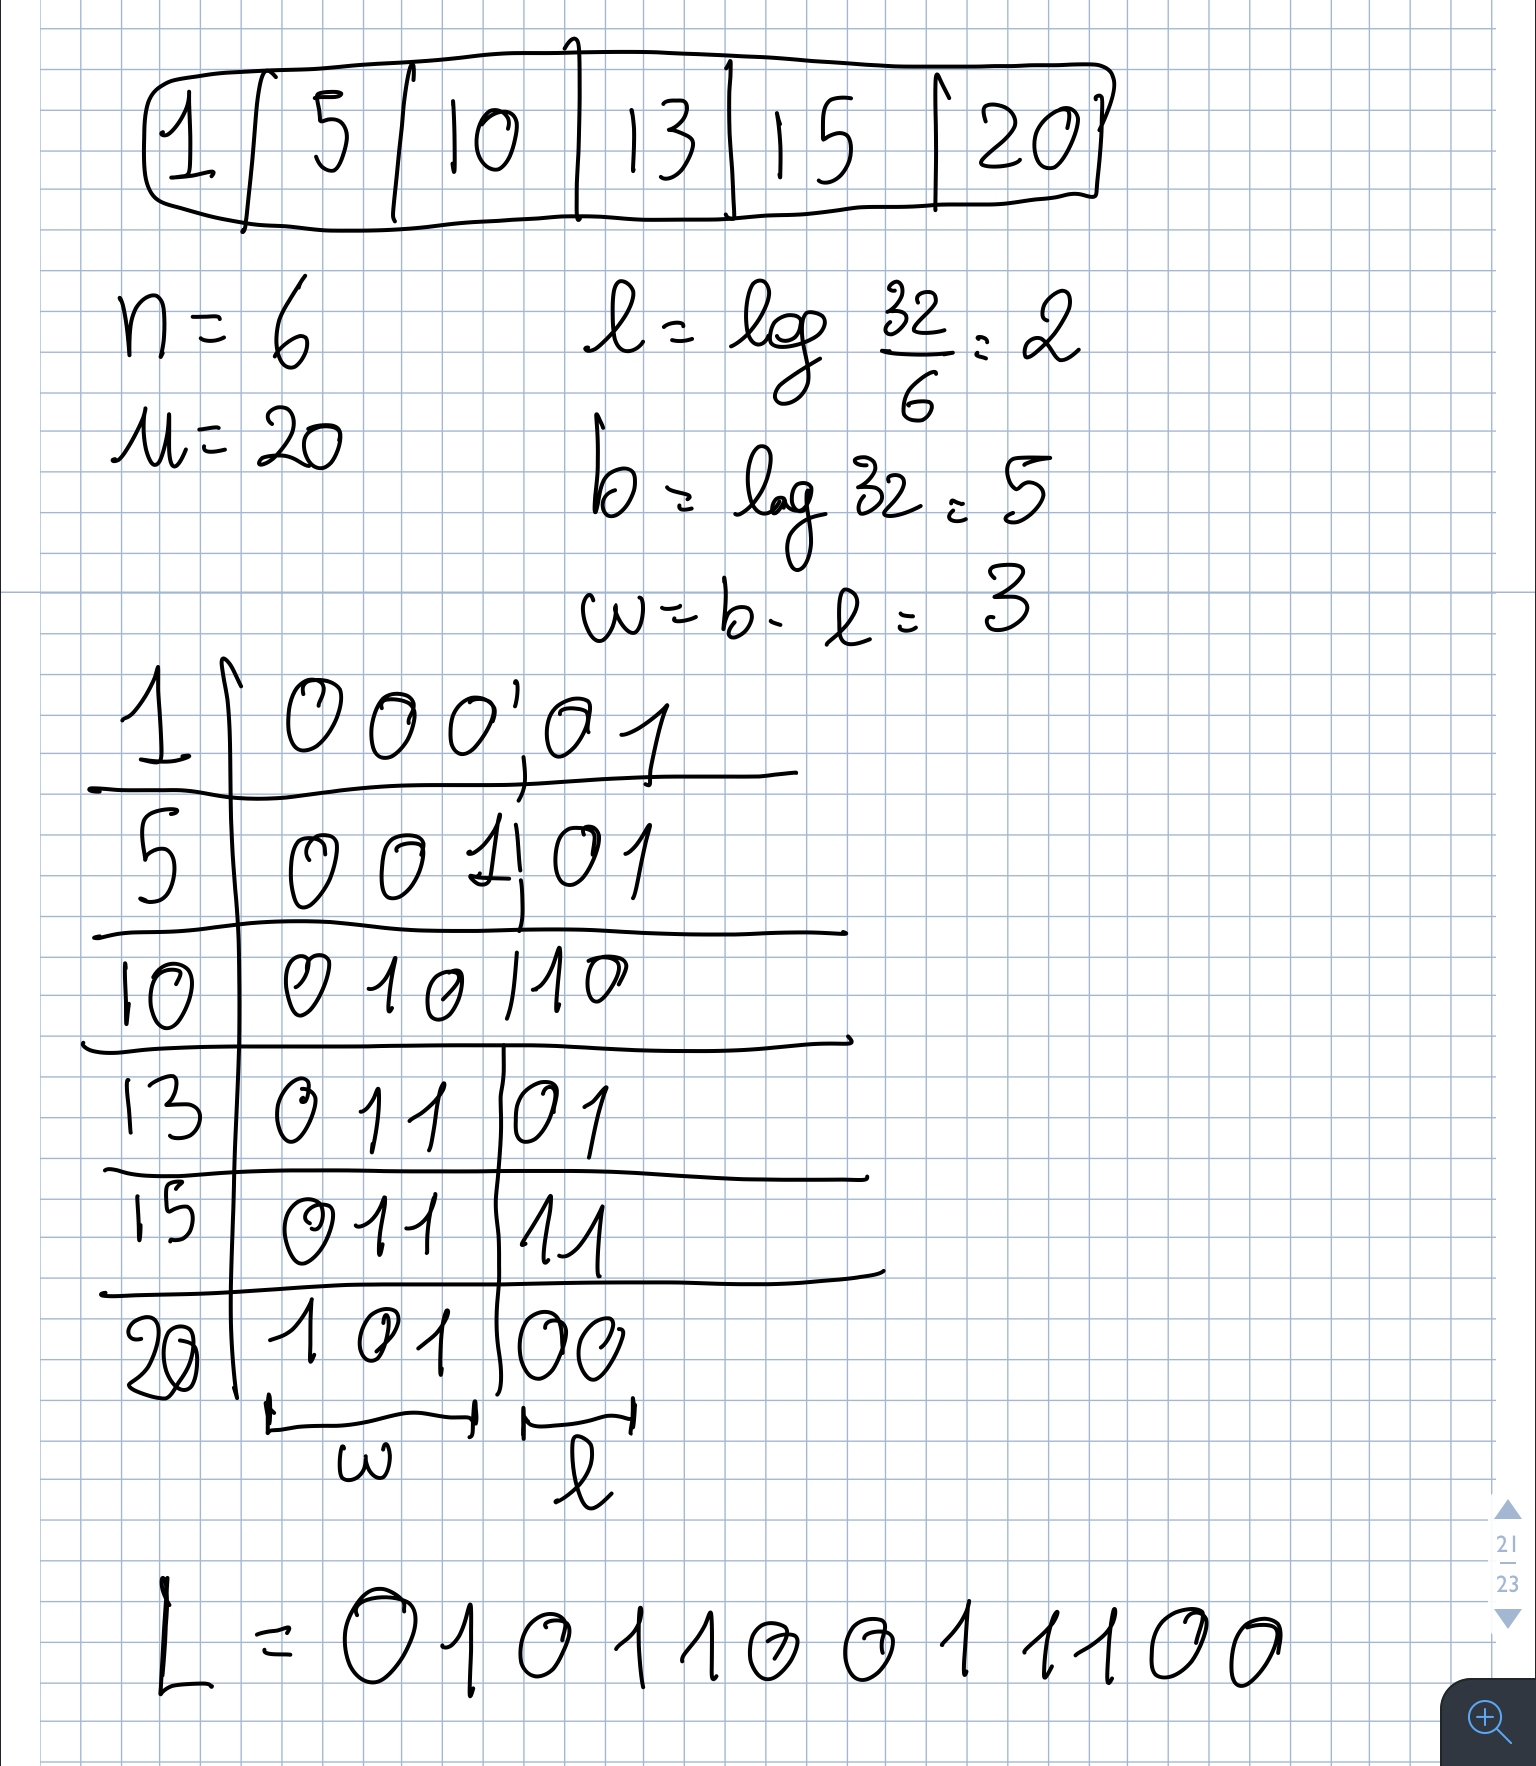
\includegraphics[width=0.7\linewidth]{EF1.jpg}
\end{figure}

\begin{figure}[H]
\centering
  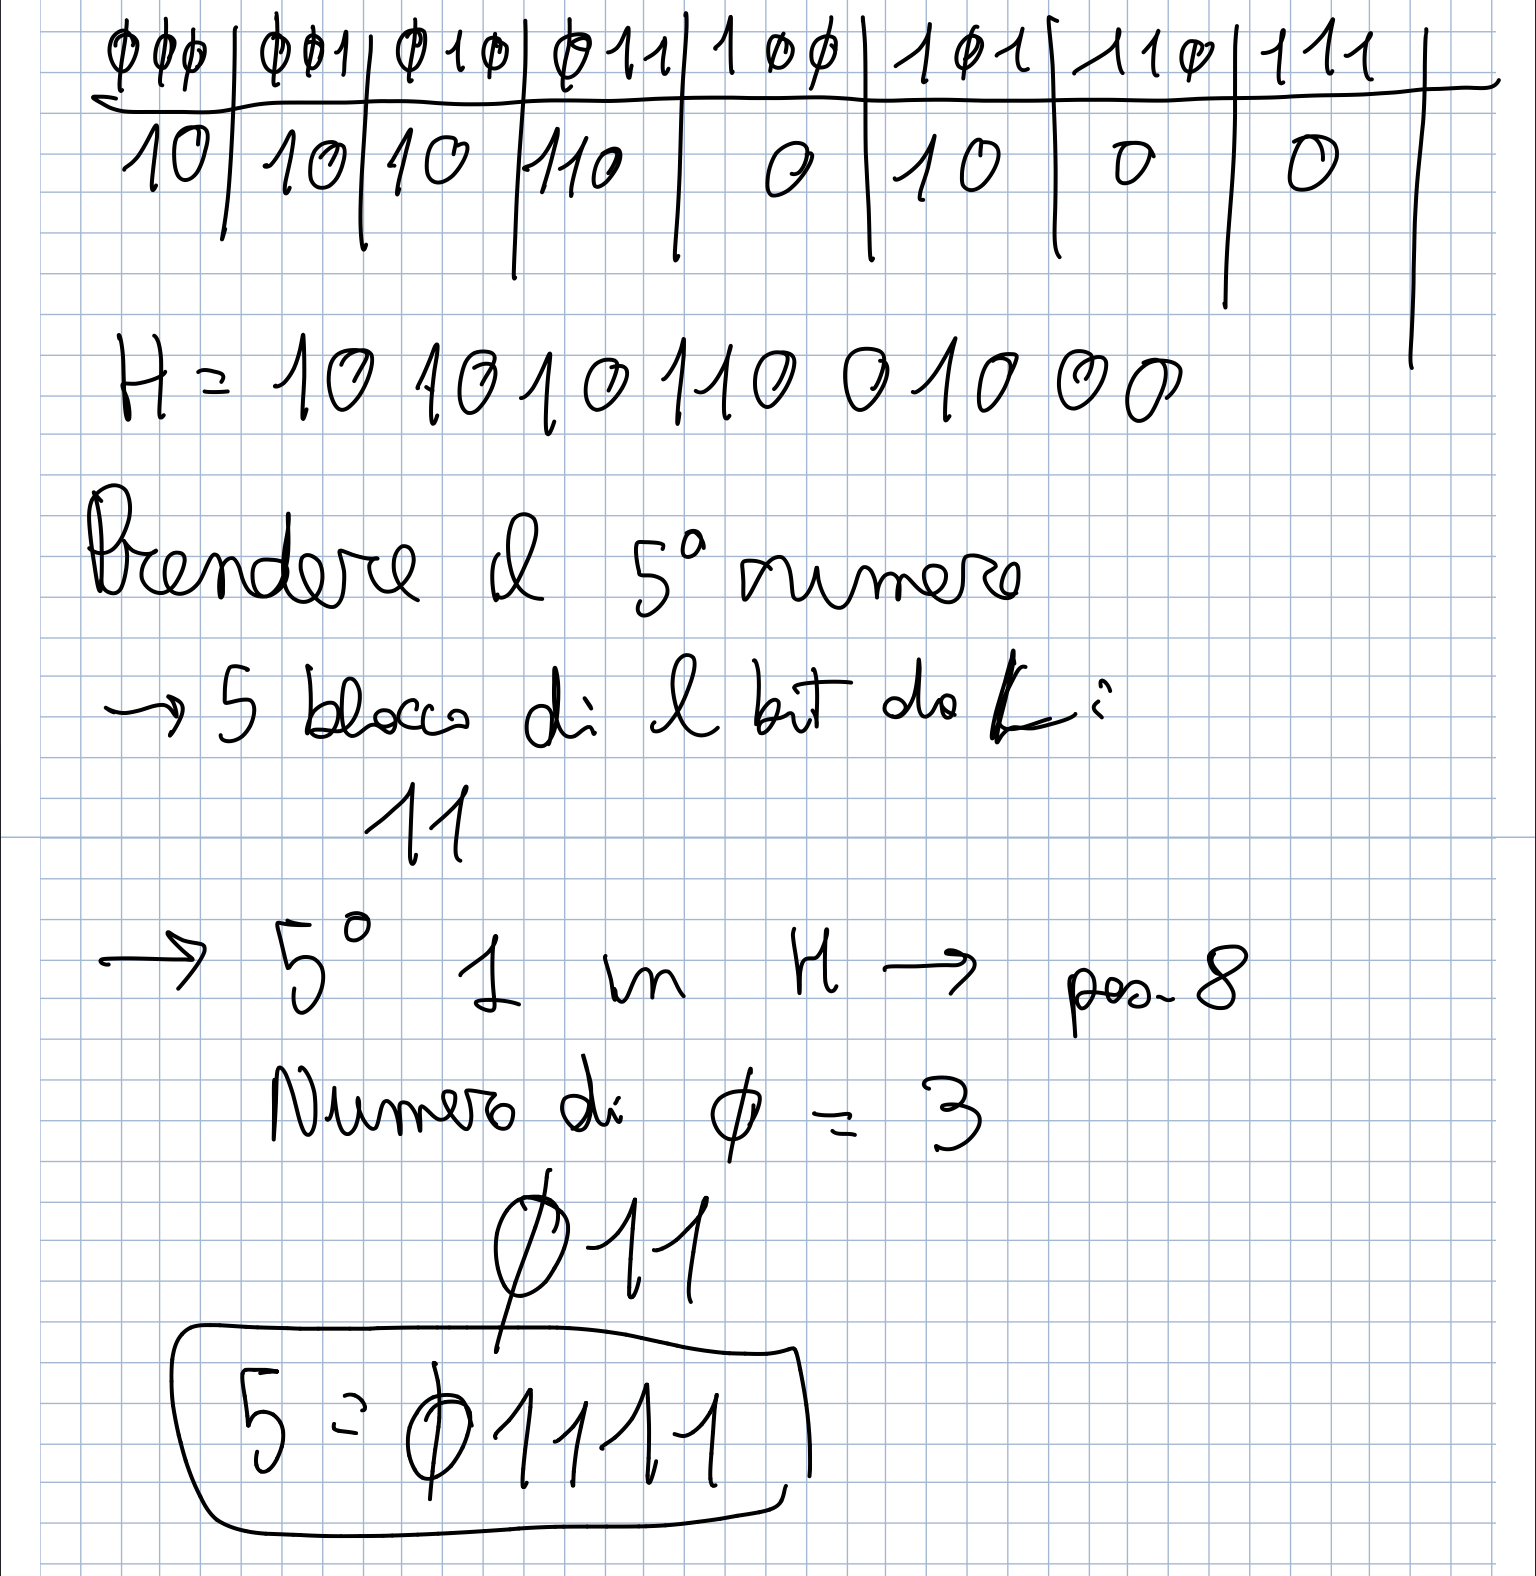
\includegraphics[width=0.7\linewidth]{EF2.jpg}
\end{figure}



\chapter{Statistical Coding}

Il problema in questo caso consiste nella compressione del testo. Abbiamo delle stringhe e ogni carattere è preso da un certo alfabeto $\Sigma$.
Una compressione statistica può essere suddivisa in due fasi:
\begin{itemize}
\item Una prima fase consiste nella creazione di un modello che sfrutta le proprietà statistiche dei vari caratteri che sono presenti all'interno della sequenza da codificare.
\item Nella seconda fase utilizziamo il modello per codificare la sequenza di input.
\end{itemize}

\section{Huffman Coding}

L'Huffman Coding è un algoritmo greedy che però è ottimo.
L'idea è quella di costruire un albero binario in cui abbiamo come foglie i vari caratteri del nostro alfabero $\Sigma$ con associata la probabilità $P[\sigma]$. 
L'algoritmo funziona in questo modo:
\begin{itemize}
\item Partiamo con una lista dei vari caratteri dell'alfabeto, ordinati in base alla probabilità $P[\sigma]$ crescente.
\item Ad ogni passaggio prendiamo i due caratteri che hanno la probabilità più bassa e li uniamo creando un nodo padre.
\item Rimuoviamo dalla lista le probabilità dei nodi che abbiamo unito e aggiungiamo la probabilità del nodo padre che corrisponde alla somma delle probabilità dei nodi figli.
\end{itemize}

In tutto si vanno a creare un numero di foglie pari al numero di caratteri dell'alfabeto, quindi $\Sigma$ e un numero di nodi interi pari a $\Sigma-1$ perchè ci fermiamo dopo $\Sigma-1$ step.
Ognuno dei nodi che viene creato viene anche labellato con 0 o con 1, quindi per ogni nodo creato avremo due archi in uscita, uno con 0 e uno con 1.

In alcuni casi possiamo avere dei caratteri che vanno uniti e che hanno una probabilità uguale, quindi potremmo fare scelte differenti che ci porterebbero ad avere degli alberi differenti.
Il problema viene risolto perchè ogni volta, in caso di caratteri con la stessa probabilità, si scelgono quelli che sono più vecchi ovvero che sono stati generati prima. Questa cosa si implementa con una seconda coda di priorità in cui però ordiniamo in base al momento della creazione del nodo e allo stesso tempo anche in base al valore della probabilità.

Esempio di creazione dell'albero dell'Huffman coding usando le due code di priorità:

\begin{figure}[H]
\centering
  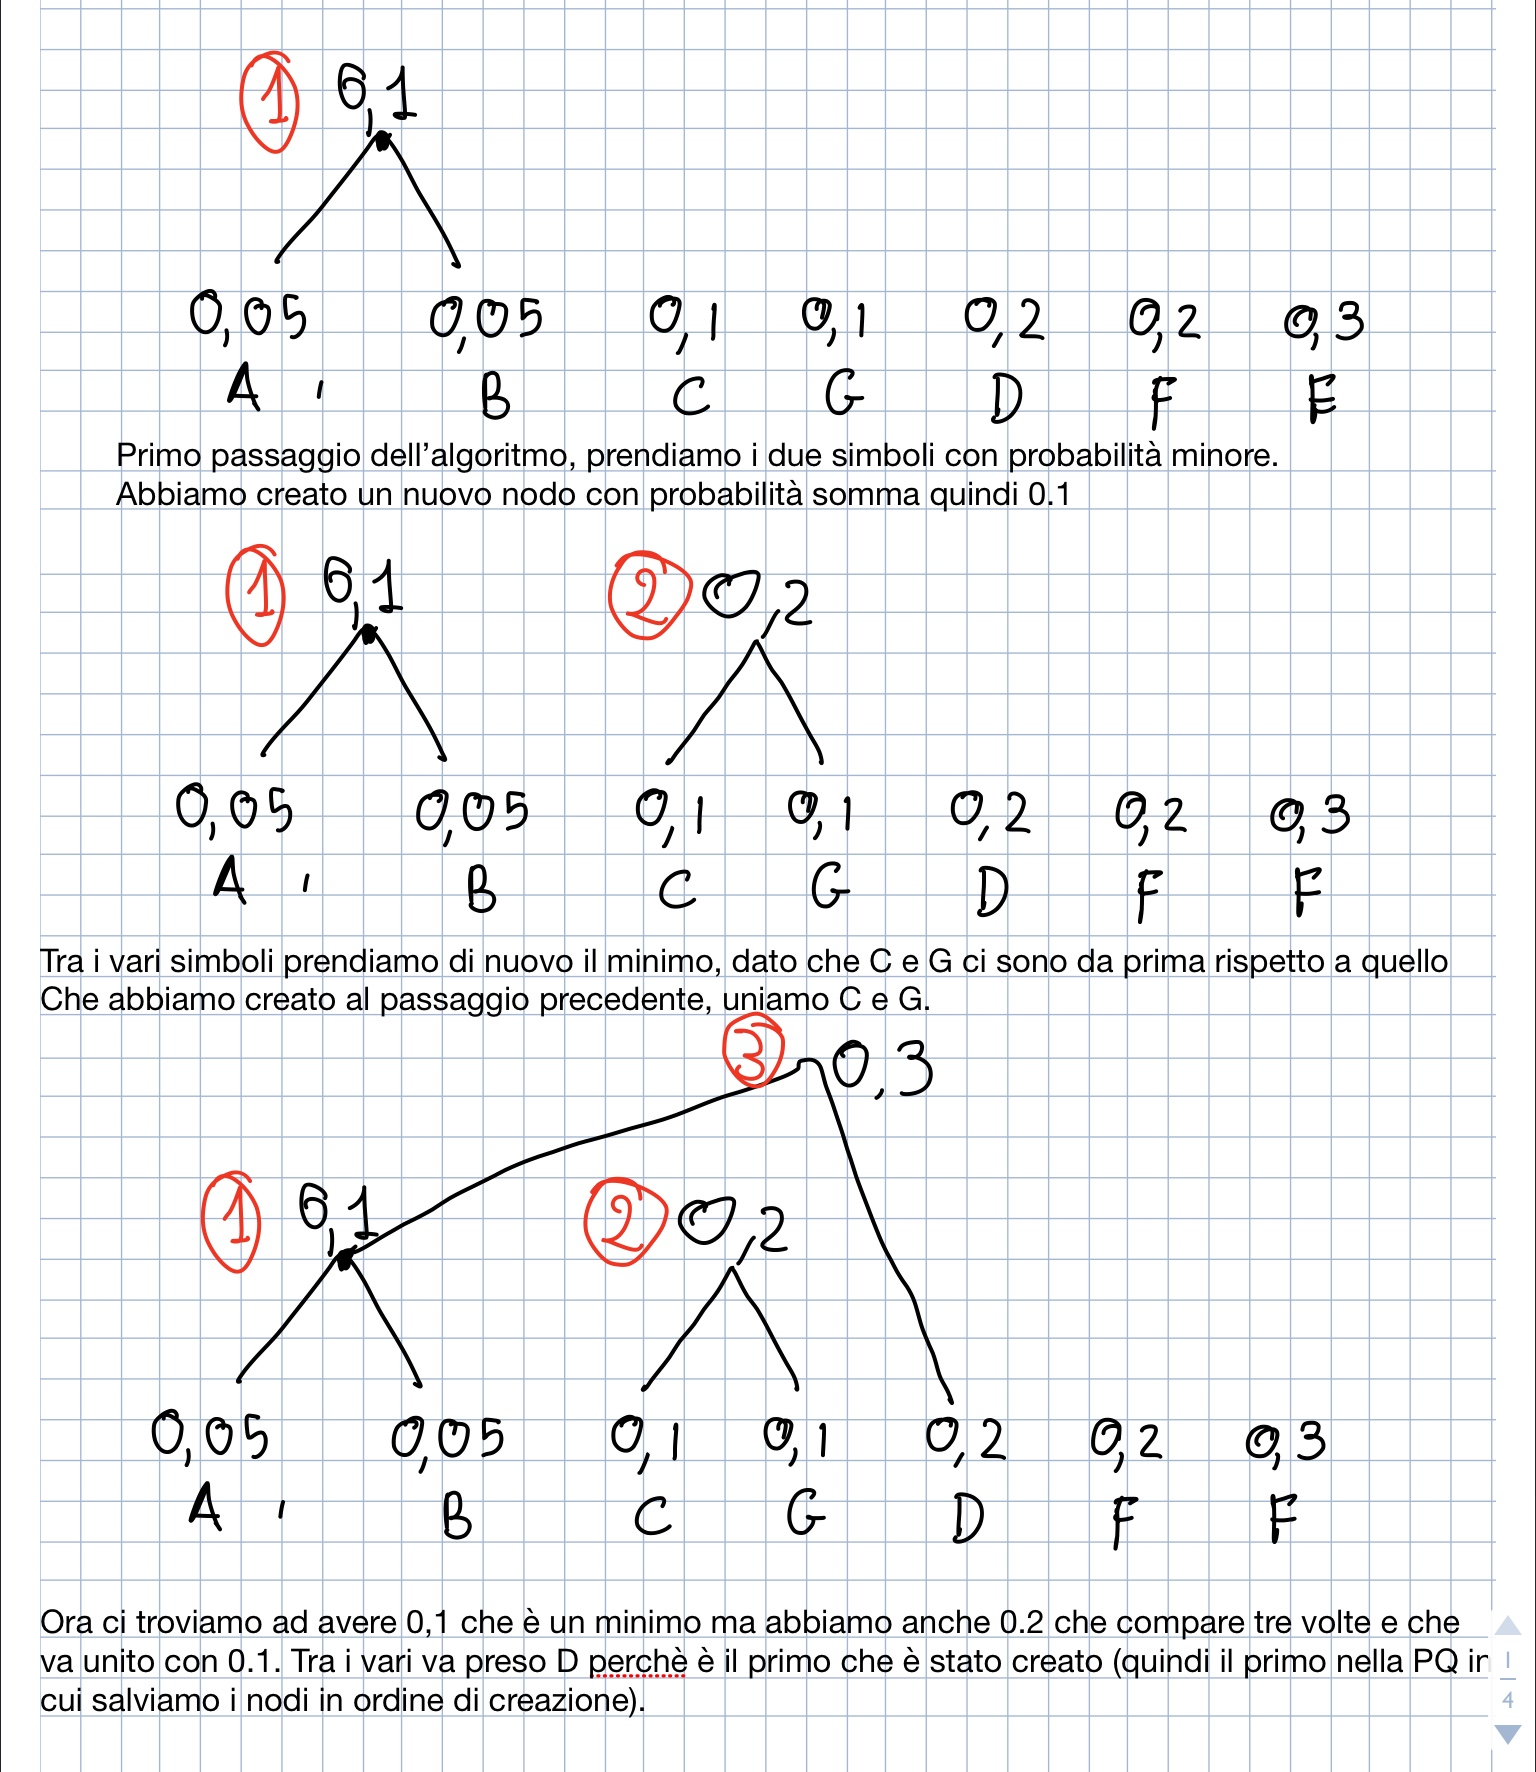
\includegraphics[width=\linewidth]{IMG_0168.jpg}

\end{figure}

\begin{figure}[H]
\centering
  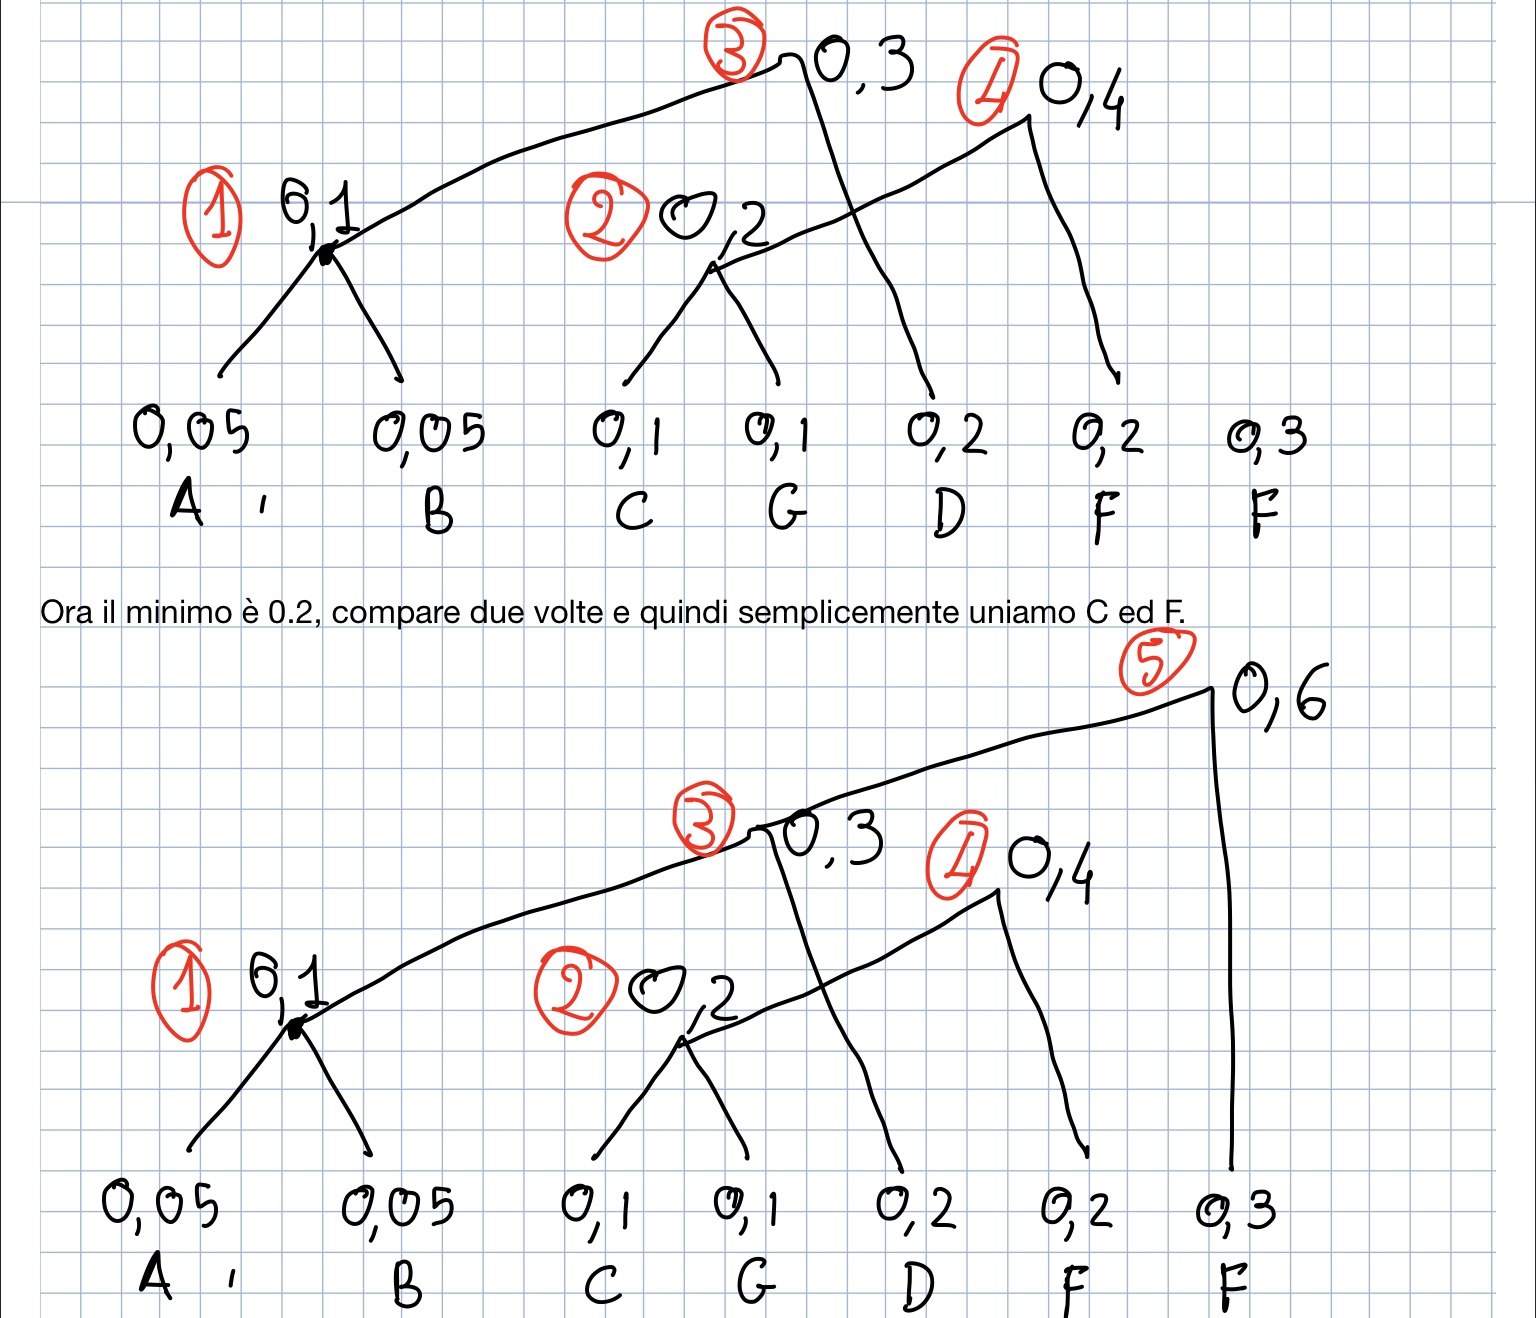
\includegraphics[width=\linewidth]{IMG_0169.jpg}

\end{figure}

\begin{figure}[H]
\centering
  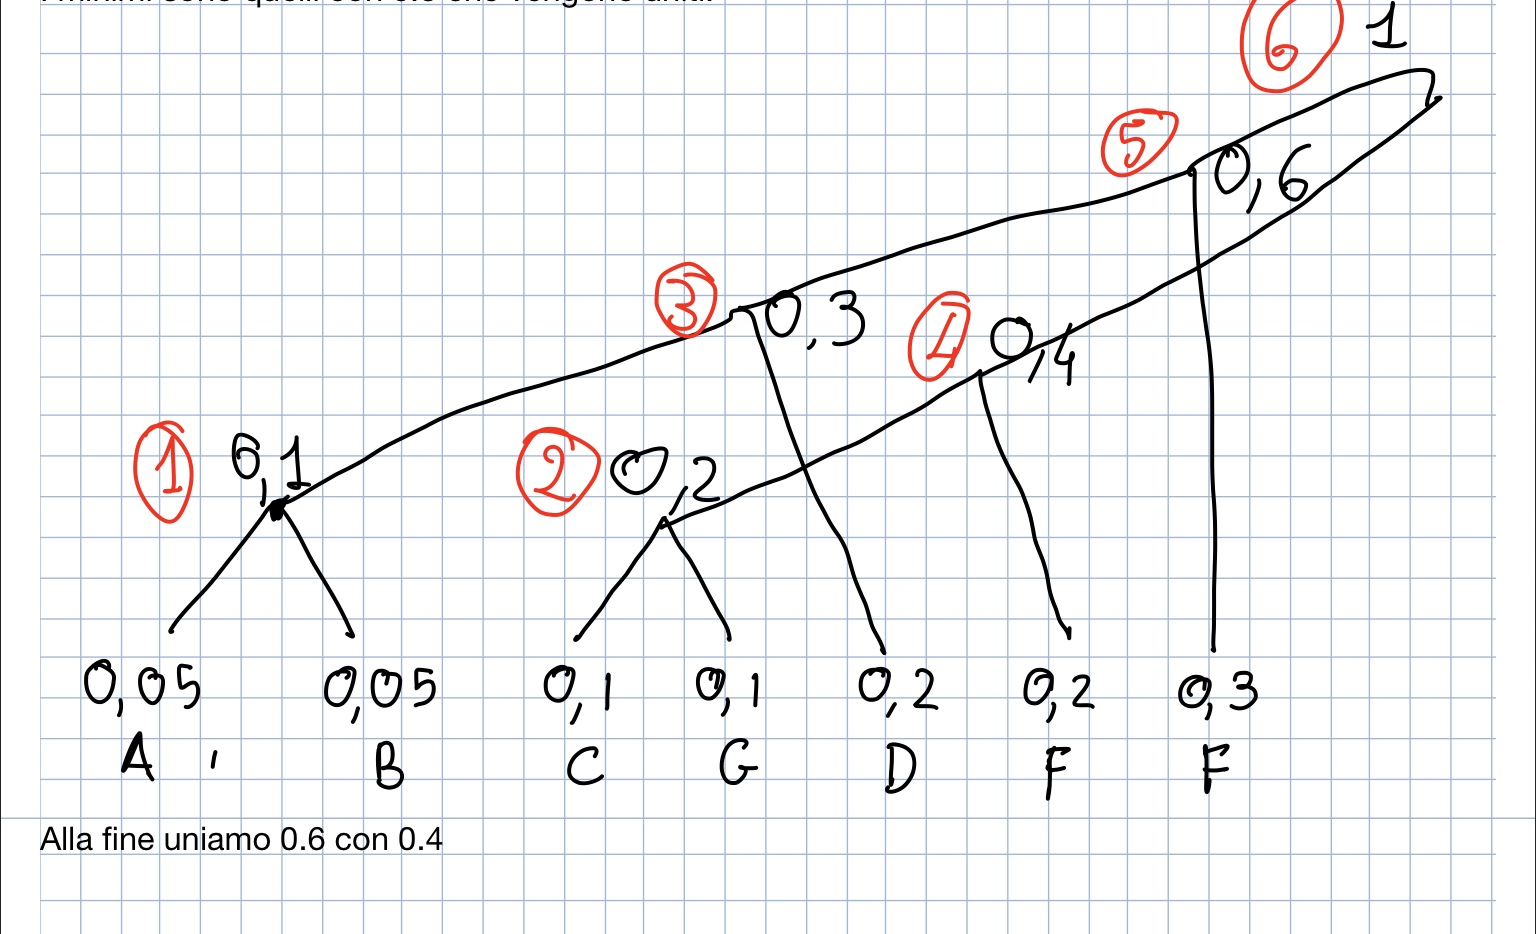
\includegraphics[width=\linewidth]{IMG_0170.jpg}

\end{figure}

Alla fine della creazione di questo albero binario, i vari caratteri che si trovano nelle foglie potranno essere codificati con l'unione dei valori che troviamo negli archi che percorriamo per andare dal nodo root alla foglia corrispondente.
Per ogni carattere $\sigma$ che vogliamo codificare, corrisponde una codifica $L(\sigma)$ che ha una lunghezza pari al percorso che faccio per andare dal nodo root alla foglia, quindi corrisponde alla profondità di quella foglia.
L'obiettivo è avere una lunghezza della codifica del carattere $L(\sigma)$ che sia la minima possibile in modo da ridurre il tempo per la compressione e per la decompressione. Questa minimizzazione la otteniamo con la tecnica del più vecchio spiegata prima.

Dato che abbiamo $\Sigma-1$ nodi interi e un alfabeto di $|\Sigma|$ caratteri allora potremo generare $2^{|\Sigma|-1}$ alberi labellati.

\textbf{Teorema:} Se prendiamo la lunghezza di tutte le codifiche dei caratteri che creiamo con l'Huffman coding abbiamo una lunghezza $L_c=\sum_{\sigma \in \Sigma} L(\sigma)P[\sigma]$.
Possiamo dire che utilizzando l'Huffman coding, questa lunghezza $L_c$ è la minore che possiamo ottenere tra tutti gli algoritmi di encoding, quindi $L_c<L_c'$ dove $c$ è l'Huffman Coding e $c'$ è un qualsiasi altro algoritmo.

Per dimostrare il teorema dobbiamo considerare che ogni albero che si crea con l'Huffman encoding è un albero binario, l'ottimalità dell'Huffman encoding la possiamo dimostrare se consideriamo che vogliamo trovare l'albero binario con la profondità minore.

Lemma: Dato di un set F di alberi binari di profondità minima costuiti da un alfabeto di n caratteri (n foglie quindi), ne esiste uno T che è quello in cui abbiamo le foglie x,y con probabilità minore che sono unite insieme in un nodo padre, alla profondità maggiore nell'albero.

Questo lemma è vero perchè altrimenti avremmo alla profondità maggiore nelle foglie una unione di due nodi, uno con la probabilità minore possibile e uno con probabilità più alta. Allo stesso tempo avremmo all'interno dell'albero un nodo che avrà probabilità minore di questo nella foglia. Scambiano la foglia con il nodo con probabilità minore otterremmo un albero che quindi avrà una profondità minore rispetto a quella dell'albero che stiamo considerando, questo però non è possibile perchè abbiamo già preso gli alberi di probabilità minima (il set F).

Consideriamo un secondo lemma, prendiamo un albero binario T che abbiamo creato con l'Huffman Code, quindi in una delle foglie a massima profondità abbiamo x e in un'altra x che vengono unite in un nodo z. Prendiamo la versione ridotta di T che è R ed è creato su $n-1$ caratteri andando a rimuovere x e y e lasciando solamente z.

Il lemma mi dice che tra l'albero T e la versione ridotta c'è la seguente relazione: $L_T = L_R\ + \ P_x + P_y$.
Dimostrazione: $L_T$ è uguale a $L_T=\sum(p_\sigma L(\sigma))+(P_x+P_y)(L_T(z)+1)$, invece $L_R=\sum(p_\sigma L(\sigma))+(P_x+P_y)(L(z))$. Quindi in pratica prendendo $L_T$ vediamo che la differenza rispetto a $L_R$ è il +1 nella moltiplicazione e quindi è dimostrata la relazione nel lemma.

Ora possiamo dimostrare il teorema e lo dimostriamo per induzione:

\begin{itemize}
\item Partiamo dicendo che vogliamo dimostrare che $L_h<L_c$ ovvero che la lunghezza che ottengo con l'encoding di Huffman è migliore di qualsiasi altro encoding. 
\item Partiamo con un alfabeto di 2 caratteri, ogni encoder e anche Huffman utilizzano 2 bit per codificare, 1 bit per ogni carattere, quindi qua abbiamo che Huffman è l'ottimo.
\item Prendiamo adesso il caso dell'alfabeto con n caratteri e consideriamo che per n-1 caratteri Huffman è l'ottimo e quindi vale $L_h \leq L_c$.
\item Nel caso n caratteri diciamo che abbiamo un encoder ottimo quindi vale $L_c \geq L_h$ abbiamo due alberi binari che sono creati dai due encoder, $T_C$ e $T_H$. Per entrambi possiamo creare la versione ridotta che viene creata su $n-1$ caratteri. Quindi abbiamo $R_C$ e $R_H$ quindi in pratica possiamo dire che vale la relazione $L_{R_H}\ \leq \ L_{R_H}$.
\item Ora consideriamo il lemma, possiamo riscrivere $L_C$ e $L_H$ come \\ 
$L_C=R_{L_C}+P_x+P_y$ \\
$L_H=R_{L_H}+P_x+P_y$ \\
Quindi vale che $L_C \leq L_H$ e quindi $L_C = L_H$ perchè valeva anche l'opposto e quindi l'Huffman Code è ottimo. 
\end{itemize}

\textbf{Teorema:} Data l'entropia $H$ definita come $H=\sum^n_1 p(\sigma)Log_2\frac{1}{p(\sigma)}$, la lunghezza media del codeword che ottengo con Huffman è $H \leq L_H \leq H+1$. \\

Questo teorema mi dice con Huffman perdiamo 1 bit per ogni simbolo che viene compresso. Se questa perdita è importante o meno dipende dal valore H dell'entropia. Se abbiamo una sequenza con un solo simbolo abbiamo una entropia pari a 0 perchè un simbolo compare con probabilità 1 gli altri con 0, in questo caso perdere 1 bit è importante.
Se invece abbiamo una sequenza con tanti simboli avremo che al massimo l'entropia avrà valore $Log_2 |\Sigma|$ e in questo caso perdere un bit non è importante.

Una possibile soluzione proposta da Shannon consiste nell'aumentare la dimensione della $\Sigma$ andando a considerare tutte le sottostringhe di dimensione k che possono essere generate, in questo modo non costruiamo una codifica sulla singola lettera ma costruiamo una codifica su blocchi di dimensione k, in questo modo perdiamo un bit per ogni blocco di dimensione k, quindi una frazione di bit per ogni carattere.
Questo approccio diventa inutilizzabile in pratica perchè se aumentiamo troppo il valore di k andiamo ad aumentare anche la dimensione dell'alfabeto e quindi aumenta anche l'encoding dell'albero binario che si crea nella prima fase dell'Huffman code.

\section{Canonical Huffman Coding}

L'huffman coding presenta due problemi principali:
\begin{itemize}
\item Si deve memorizzare tutta la struttura ad albero che può diventare molto grande se aumenta la dimensione di $\Sigma$
\item La decodifica può essere lenta se devo attraversare tutto l'albero, inoltre la visita di ogni arco può comportare anche un cache miss.
\end{itemize}

Per risolvere queste due problematiche è stato utilizzato il Canonical Huffman. Vogliamo trasformare l'albero binario in una nuova forma che non necessita i puntatori e quindi trasformiamo l'albero in uno heap.

Il canonical Huffman Coding inizialmente crea l'albero come nella classica codifica di Huffman e per ogni simbolo $\sigma$ si calcola la corrispondente lunghezza $L(\sigma)$ della rappresentazione codificata. 
Canonical Huffman Coding utilizza le seguenti strutture dati:
\begin{itemize}
\item Un array $num$ in cui $num[l]$ indica la quantità di simboli che hanno una codifica di lunghezza l
\item Un array $symb$ in cui $symb[l]$ è una lista in cui inseriamo i simboli che vengono codificati con una codifica di lunghezza l
\item Un array firstCode in cui in $fc[l]$ memorizziamo la codifica del primo simbolo codificato con l bit.
\end{itemize}

È importante notare come viene costruito l'array $fc$, $fc[l]=x$ indica il codeword che rappresenta x in l bit, ad esempio se abbiamo $fc[5]=4$ vuol dire che dobbiamo trovare il codeword che in 5 bit rappresenta 4 che sarebbe $00100$.
Quindi, l'ultimo elemento dell'array $fc[max]$, che è relativo alla rappresentazione più lunga che abbiamo con il canonical Huffman code avrà valore 0. I precedenti invece dipendono dal valore del successivo e dal corrispondente valore nell'array num.
\begin{code}
\begin{lstlisting}[escapeinside={(*}{*)}]
fc[max] = 0
for(l=max-1;i>=1;i--):
    fc[l]=(fc[l+1]+num[l+1])/2
\end{lstlisting}
\end{code}

In quanto a spazio per memorizzare la tabella symb abbiamo bisogno di $(|\Sigma|+max)Log_2(|\Sigma|+1)$ bit e per l'array num invece abbiamo bisogno di $max^2$ bit.
Non usiamo puntatori e ammesso che fc sia abbastanza piccola non abbiamo dei cache miss durante la decodifica.

Ammesso di avere una sequenza di bit da codificare, la decodifica funziona in questo modo:
\begin{code}
\begin{lstlisting}[escapeinside={(*}{*)}]
v = nextBit()
l = 1
while(v < fc[l]):
    v = 2*v + nextBit()
    l++
return symb[l,v-fc[l]]
\end{lstlisting}
\end{code}

Dove nextBit() è la funzione che ci restituisce il prossimo bit della sequenza.
Un esempio:  

\begin{figure}[H]
\centering
  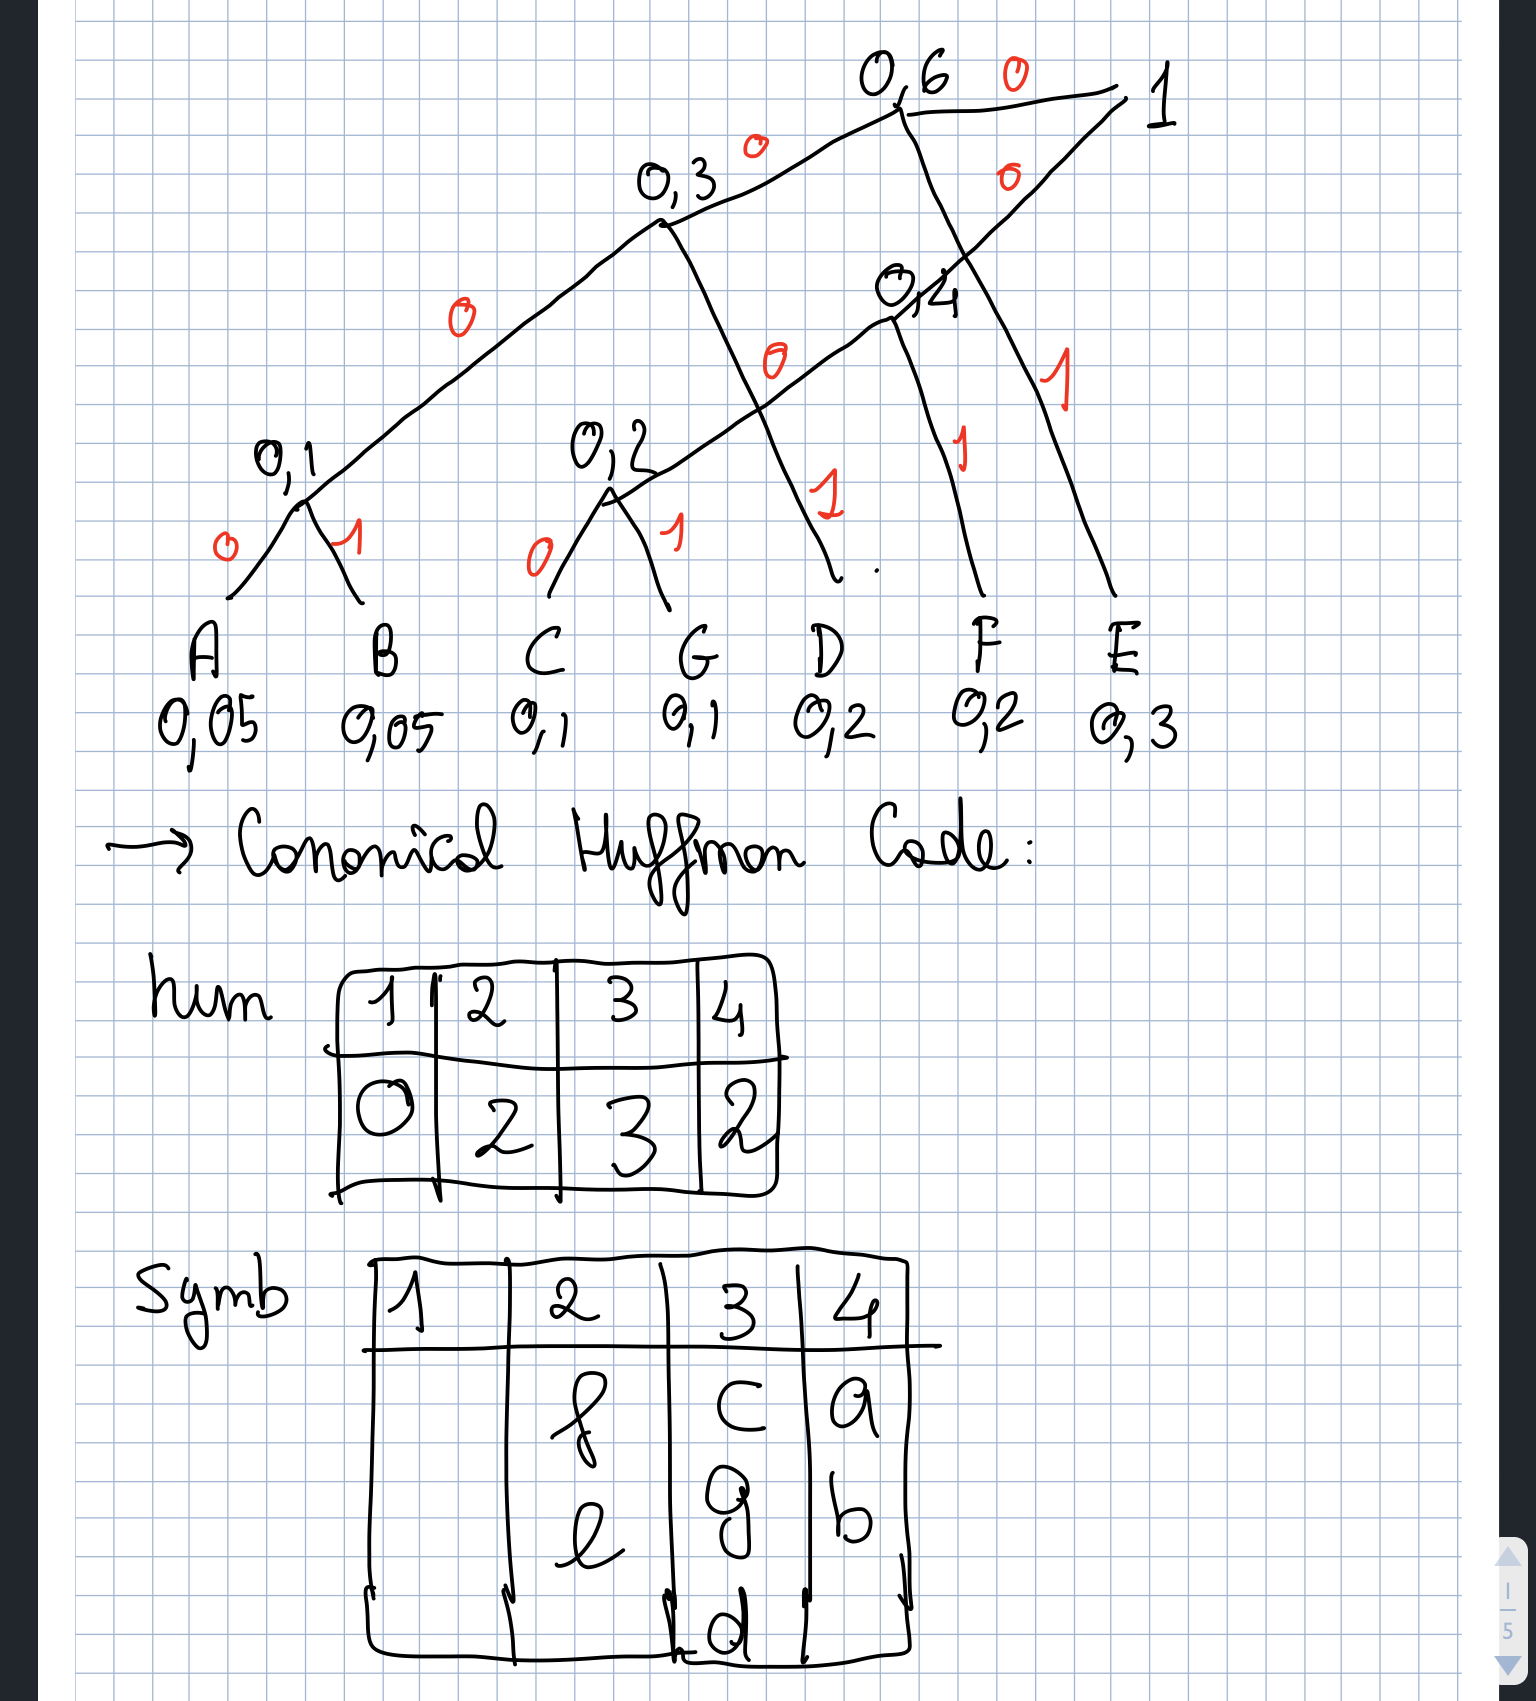
\includegraphics[width=0.7\linewidth]{IMG_0171.jpg}

\end{figure}
\begin{figure}[H]
\centering
  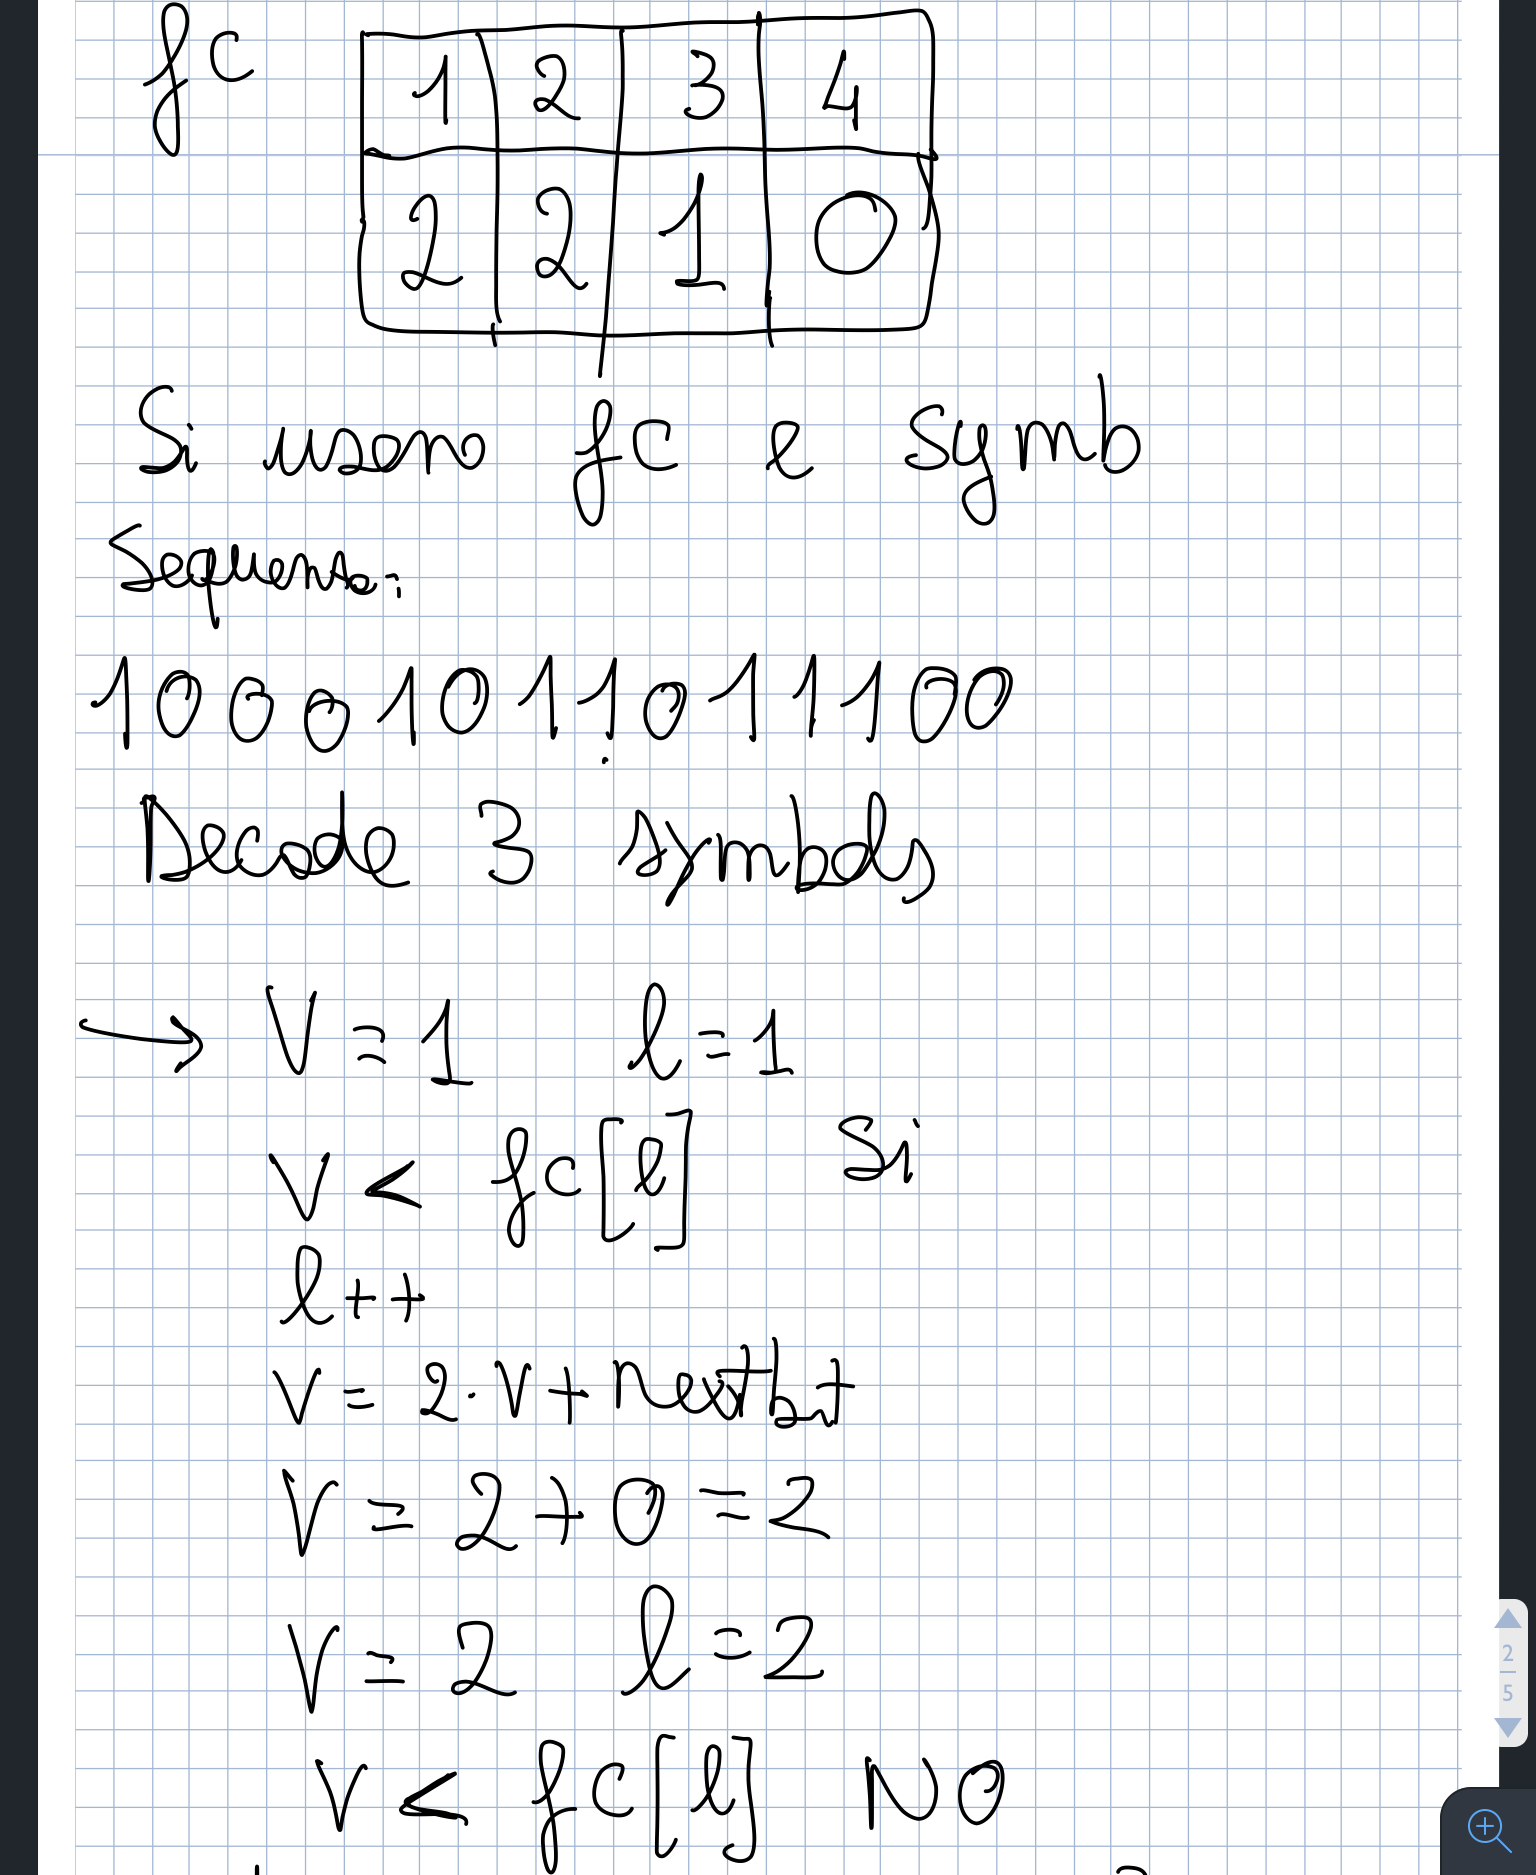
\includegraphics[width=0.7\linewidth]{IMG_0172.jpg}

\end{figure}
\begin{figure}[H]
\centering
  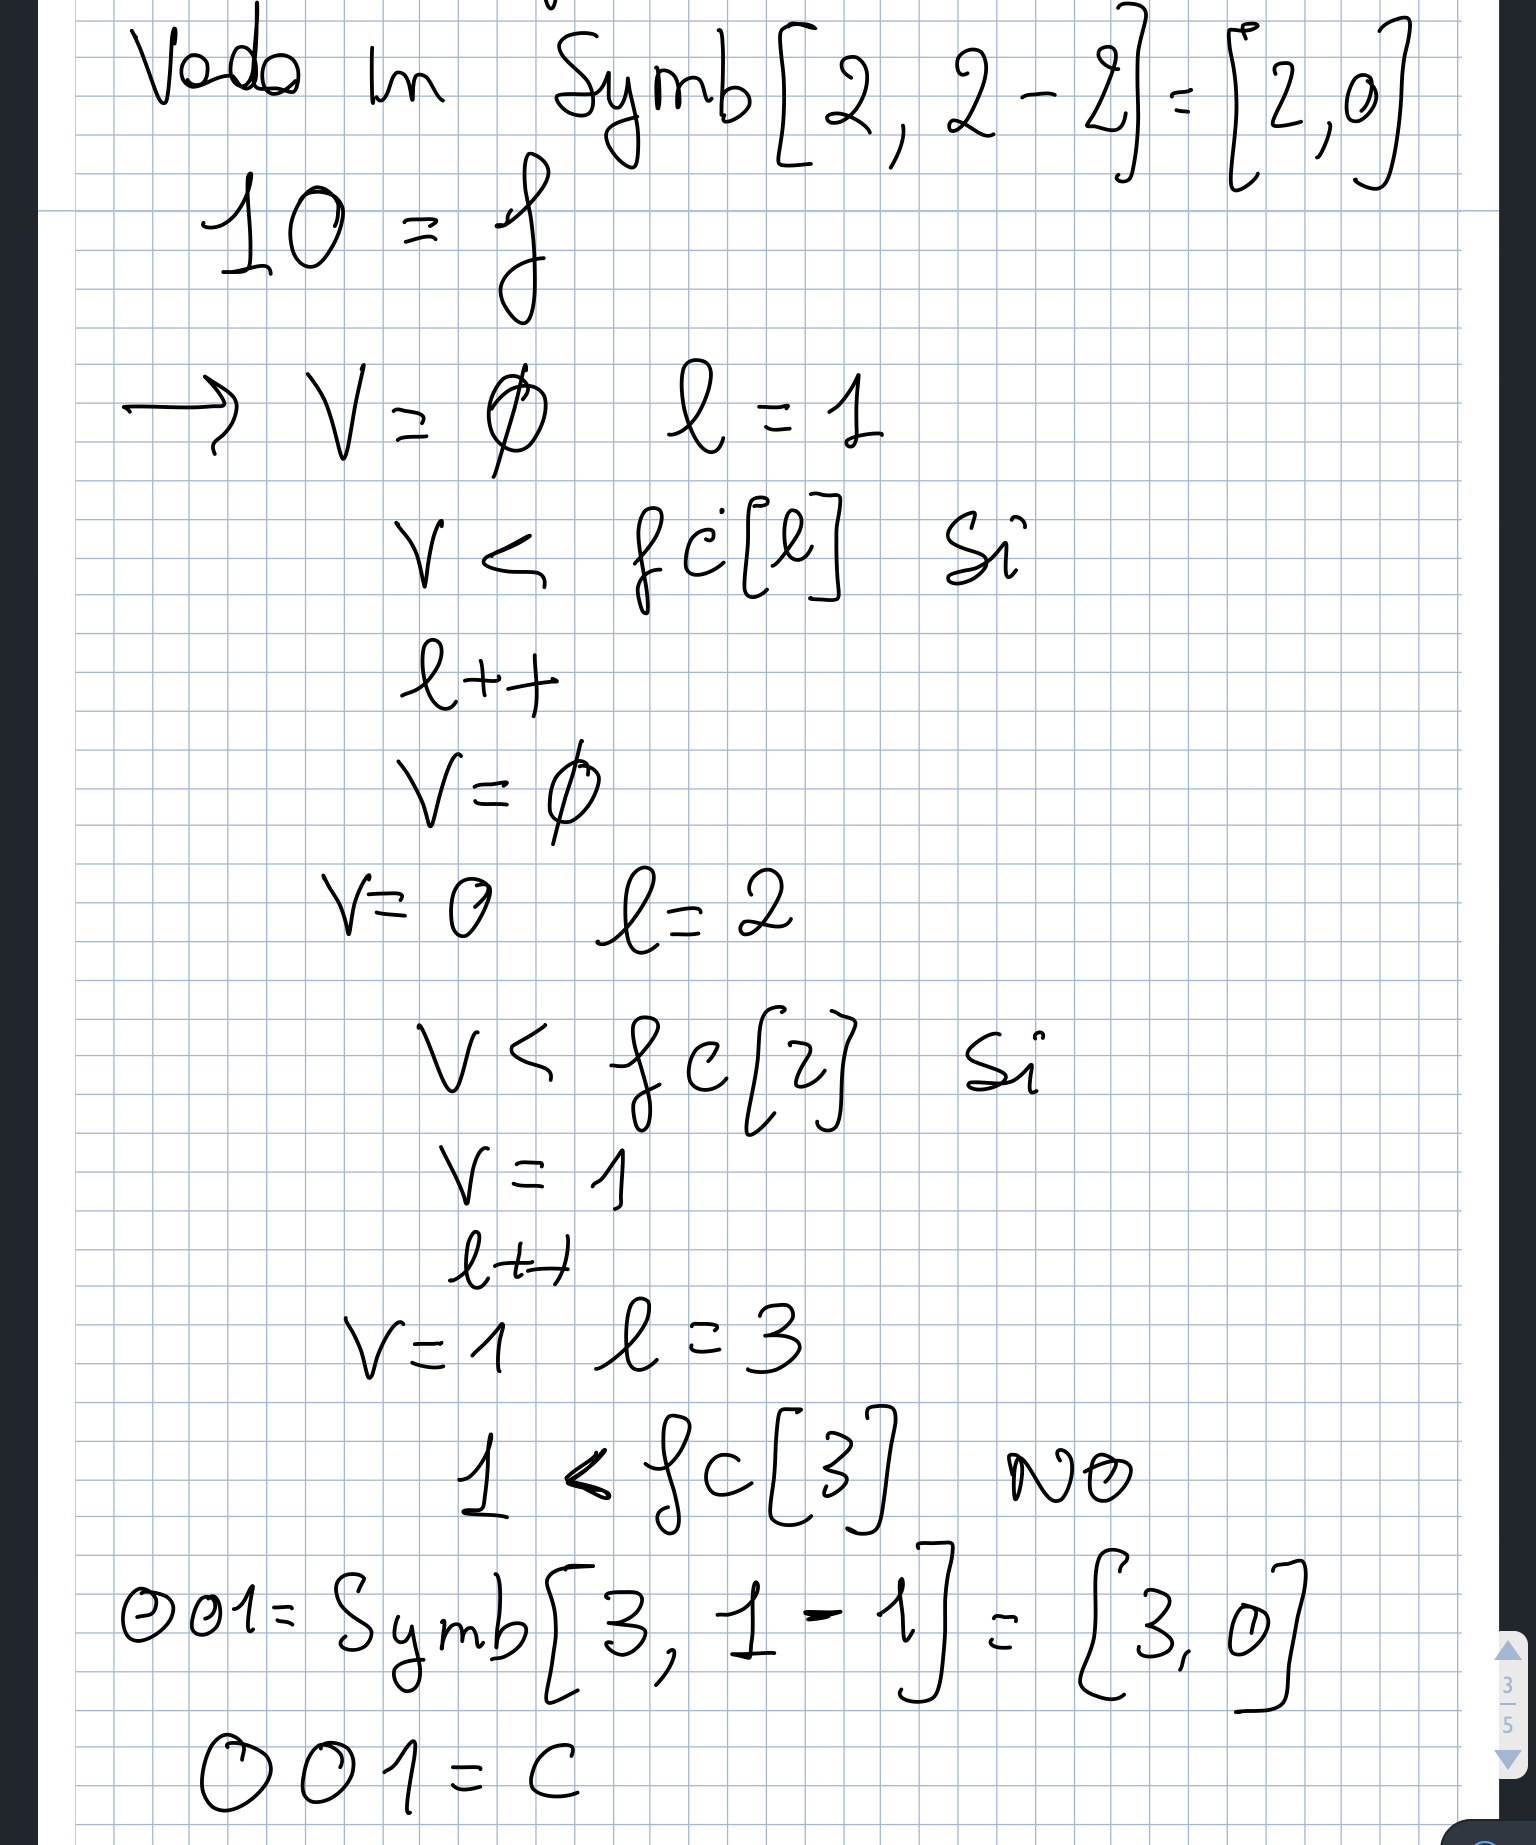
\includegraphics[width=0.7\linewidth]{IMG_0173.jpg}

\end{figure}
\begin{figure}[H]
\centering
  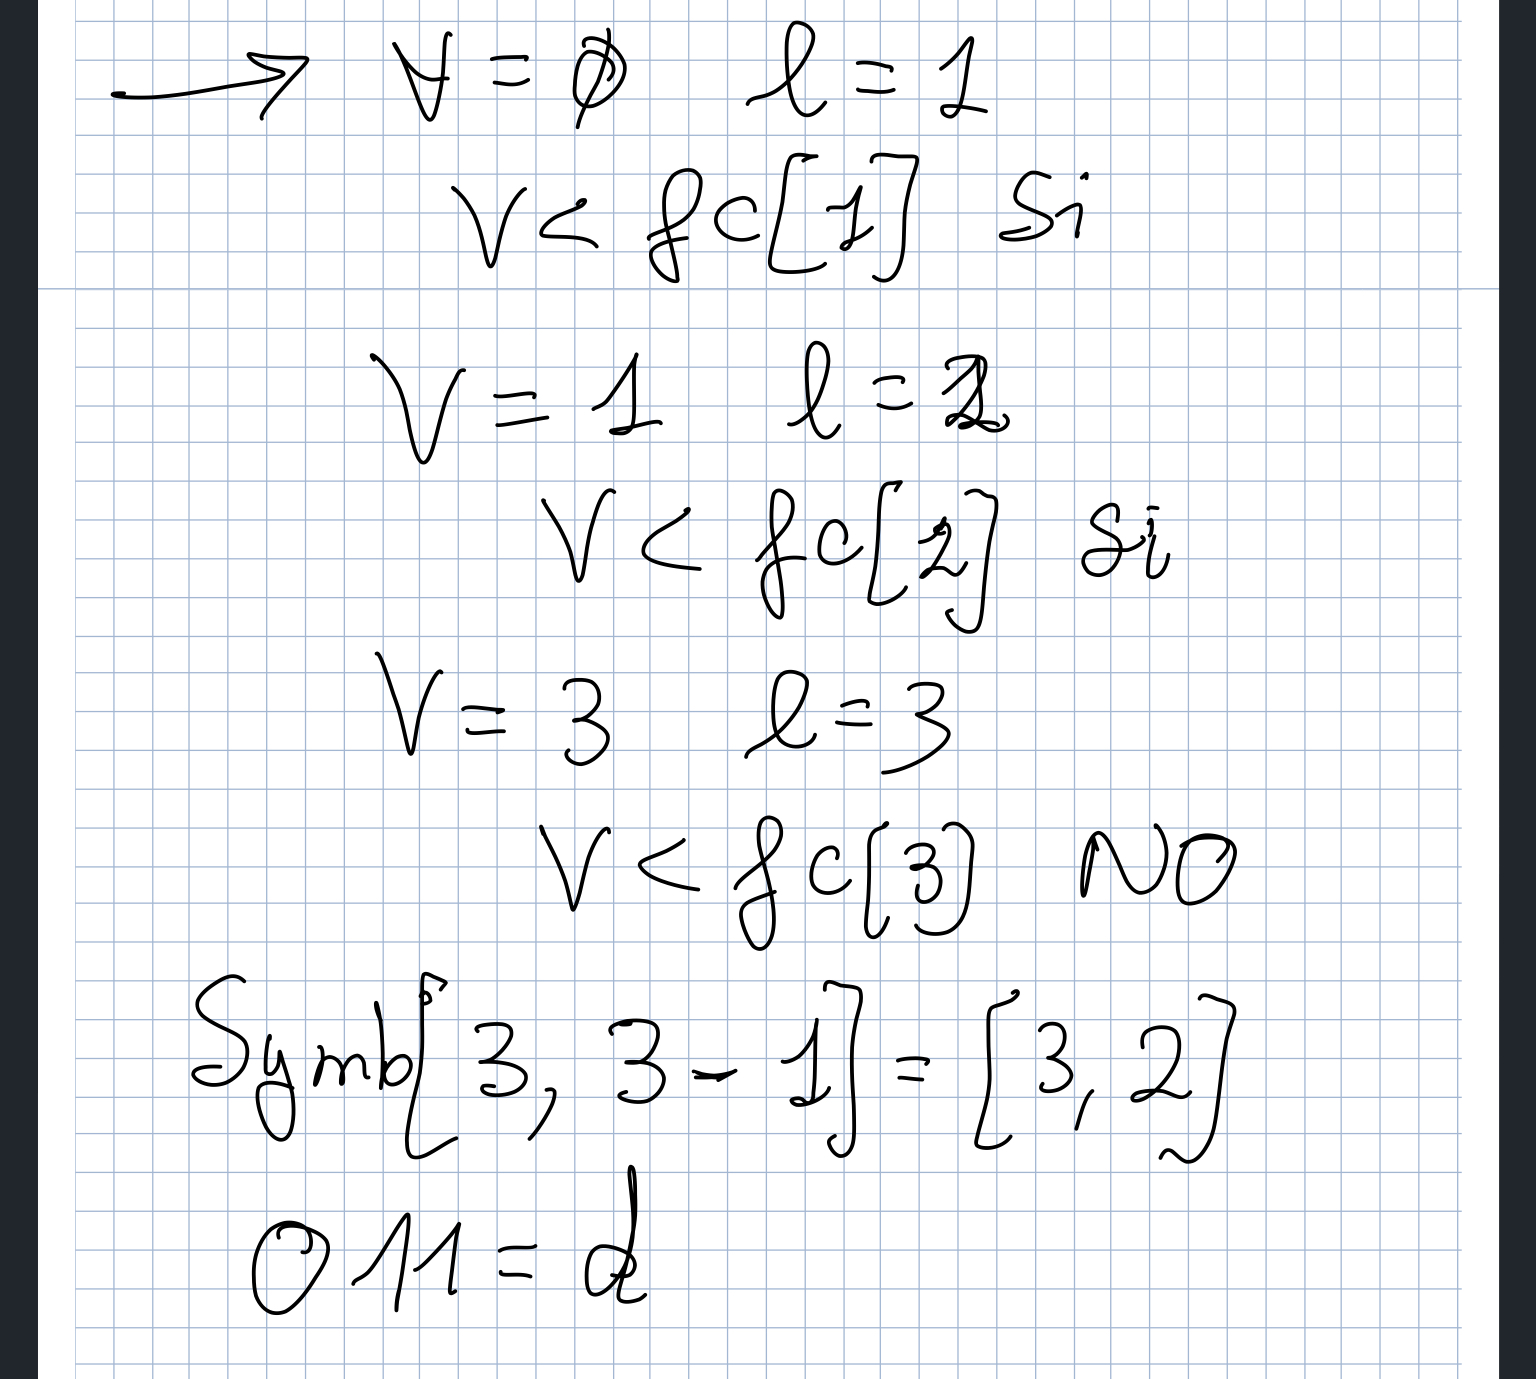
\includegraphics[width=0.7\linewidth]{IMG_0174.jpg}

\end{figure}


\section{Arithmetic Coding}

Il problema principale dell'Huffman Code è che viene sprecato 1 bit anche quando l'entropia è vicina a 0. L'arithmetic coding risolve questo problema perchè può codificare dei simboli creando una sequenza di lunghezza vicina alla 0-order entropy.
Quindi abbiamo che $H \ \leq \ L_A \ \leq \ H + \frac{1}{n}$.

Riusciamo ad ottenere questa riduzione della lunghezza della sequenza codificata perchè nell'Arithmetic coding l'output non è semplicemente una sequenza di codeword concatenati, ogni bit dell'output può rappresentare più di un simbolo in input.

\subsection{Stream di bit e frazioni diadiche}

Uno stream di bit può essere interpretato come un numero reale nel range $[0,1)$ inserendo 0, davanti alla sequenza.
Ad esempio abbiamo:\\
$0.b_1b_2b_3... = \sum_i b_i*2^{-i}$
E partendo da un numero come ad esempio 0.1101 possiamo ottenere la frazione diadica corrispondente ovvero $\frac{v}{2^k}$ dove la v rappresenta il valore della sequenza binaria mentre k indica la lunghezza della sequenza.
Per ottenere una codifica di questo genere dobbiamo partire da un numero che sia compreso tra $[0,1)$, il codice è il seguente, ci fermiamo se raggiungiamo un output periodico o quando abbiamo già un output lungo abbastanza:

\begin{code}
\begin{lstlisting}[escapeinside={(*}{*)}]
while(!accuracy):
    x = 2*x
    if(x<1):
        output = output::0
    else 
        output = output::1
        x--
\end{lstlisting}
\end{code}

\section{Algoritmo di compressione}

L'algoritmo di compressione dell'arithmetic coding è il seguente:

\begin{code}
\begin{lstlisting}[escapeinside={(*}{*)}]
$s_0$ = 1
$l_0$ = 1
i = 1
while i $\leq$ n:
    $s_i$ = $s_{i-1}$*P[S[i]]
    $l_i$ = $l_{i-1}$ + $s_{i-1}$*f[S[i]]
    
output = $<x \in [ln, ln+sn), n>$
\end{lstlisting}
\end{code}

La procedura è iterativa e vengono svolte le seguenti operazioni:
\begin{itemize}
\item Partiamo con una stringa da codifica che è formata da caratteri che sono in un alfabeto e per ogni carattere abbiamo una probabilità che compaia. Poi Calcoliamo anche la probabilità cumulativa, $f[a]=0$, $f[b]=P[a]$, $f[c]=P[a]+P[b]$ ecc.
\item Ora ad ogni iterazione si prende un carattere dalla stringa da codificare e si calcola $s_i$ e $l_i$.
\item Arrivati alla fine avremo in output $<x \in [ln, ln+sn), n>$, quindi non avremo una coppia ma un intero x che è all'interno del range e la lunghezza della sequenza codificata.
\end{itemize}

Il loop viene ripetuto un numero di volte pari alla lunghezza della sequenza che vogliamo codificare.
Graficamente lo possiamo vedere come una divisione di un certo intervallo che ad ogni iterazione viene di nuovo suddiviso in n parti.
Un esempio di codifica:

\begin{figure}[H]
\centering
  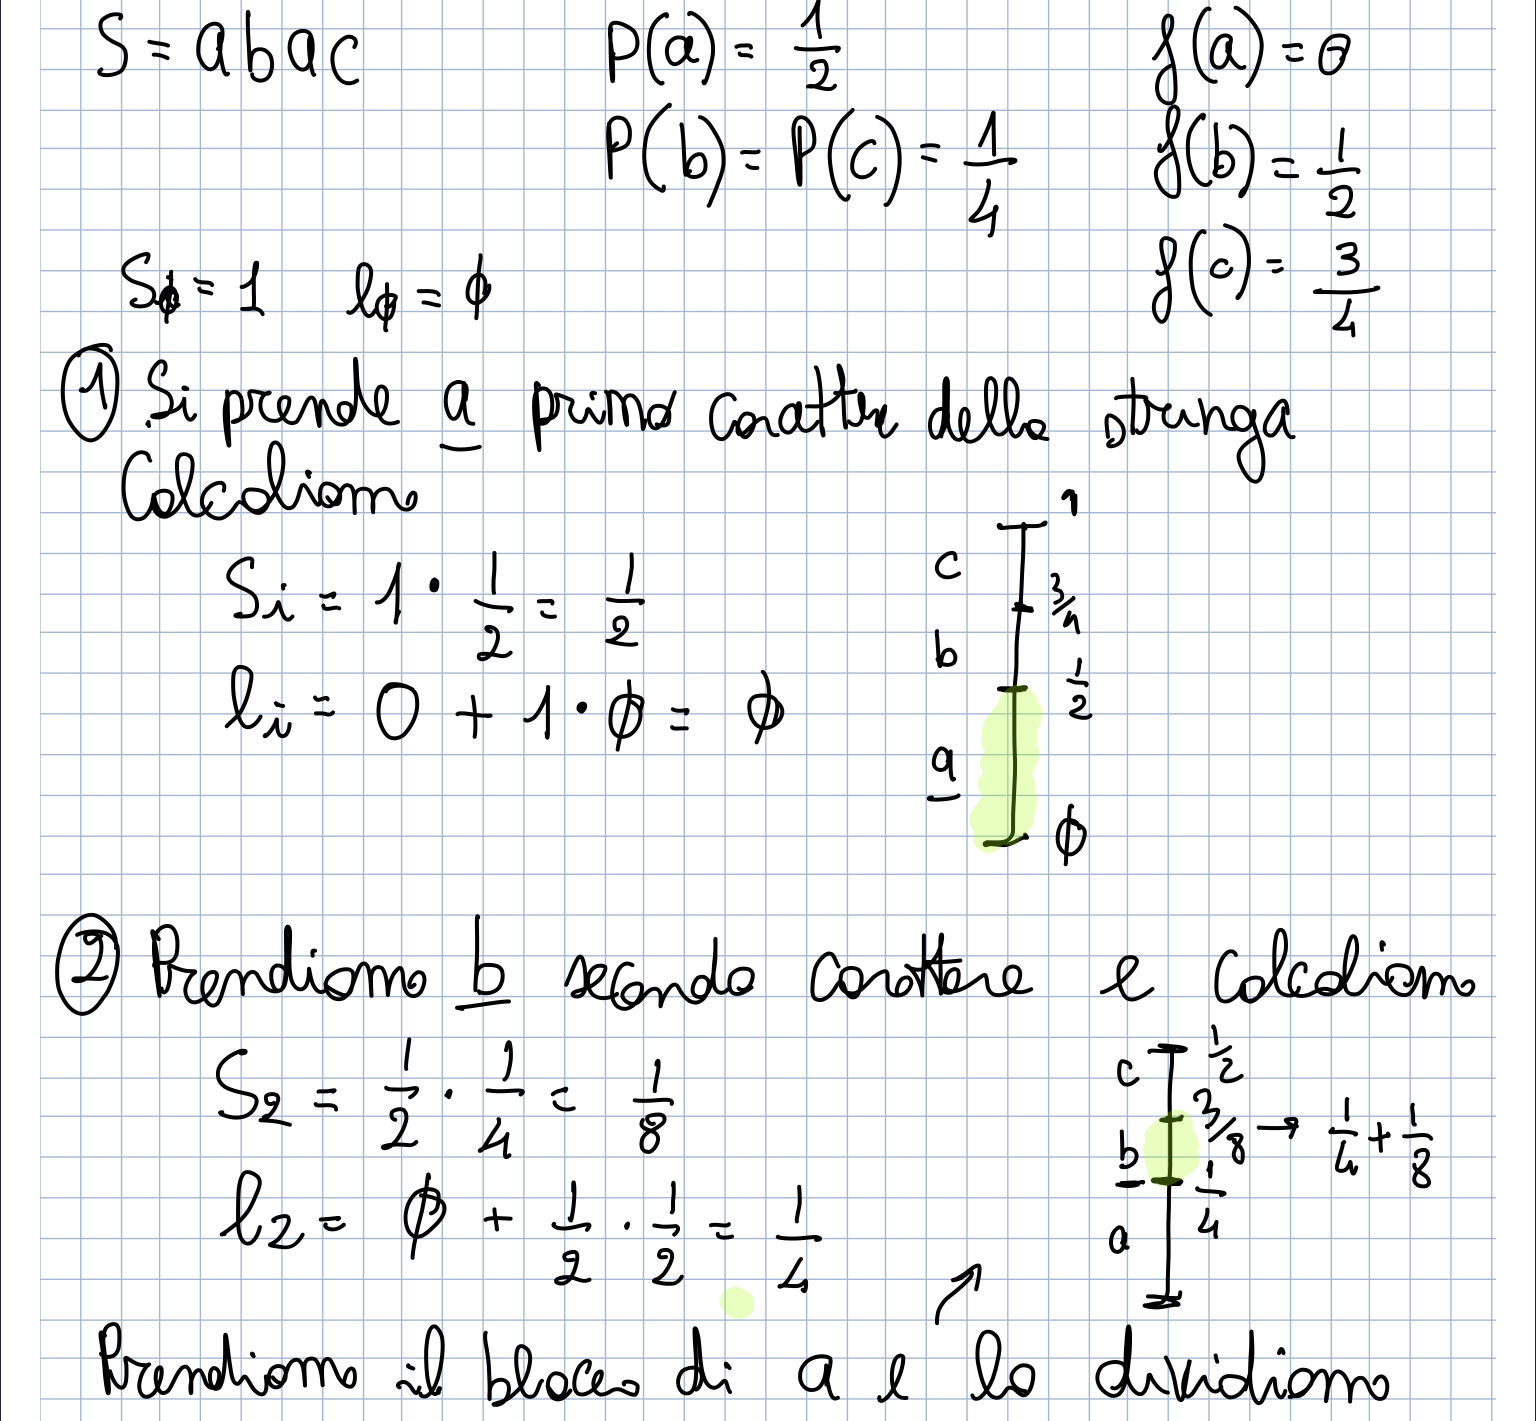
\includegraphics[width=\linewidth]{IMG_0175.jpg}
\end{figure}

\begin{figure}[H]
\centering
  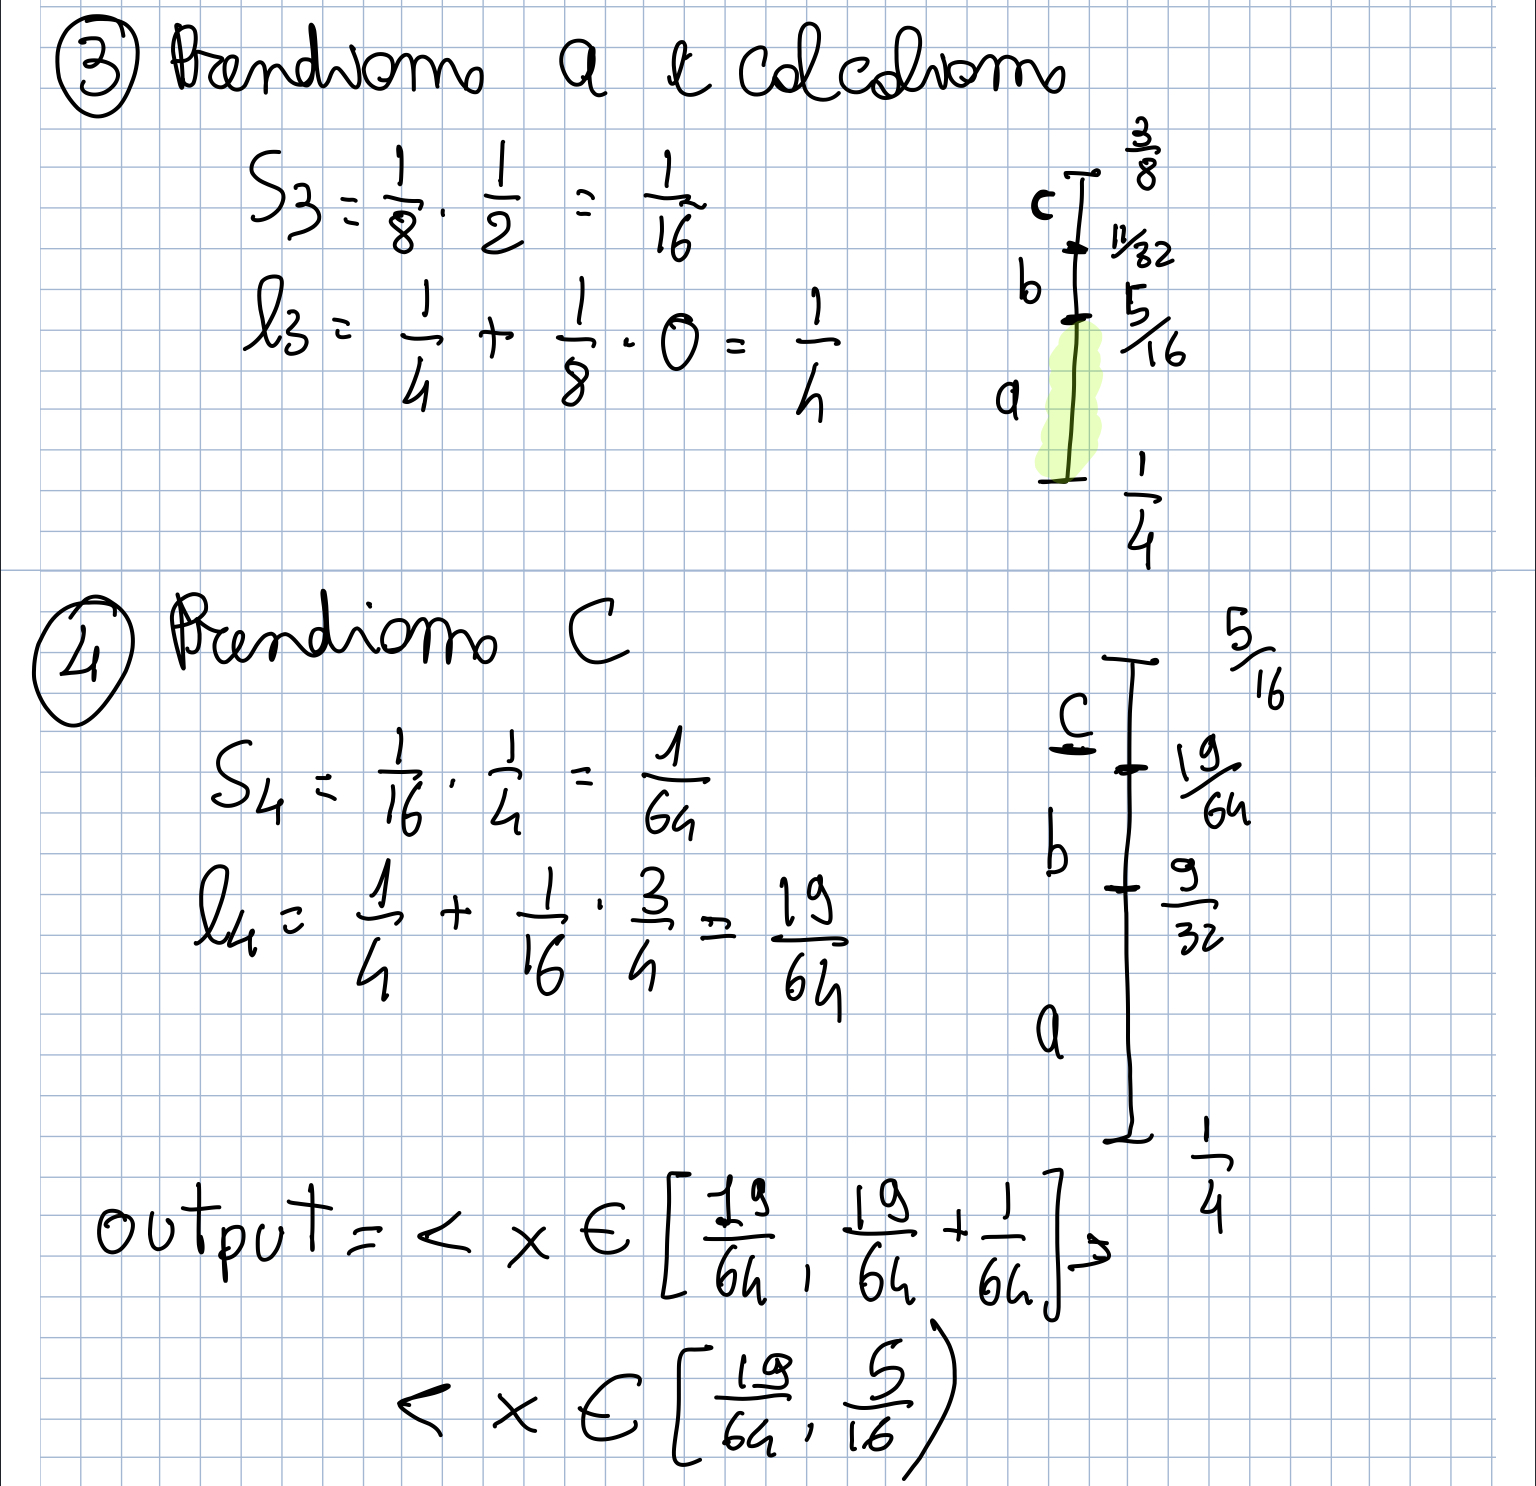
\includegraphics[width=\linewidth]{IMG_0176.jpg}
\end{figure}

\section{Decompressione}

L'algoritmo di decompressione ha bisogno di:
\begin{itemize}
\item Uno stream di bit che è stato creato dalla compressione
\item La lunghezza della sequenza compressa
\item La probabilità dei vari caratteri della sequenza compressa
\end{itemize}

La decompressione funziona in questo modo:
\begin{itemize}
\item Ad ogni iterazione suddividiamo l'intervallo in intervalli più piccoli e proporzionali rispetto alla probabilità dei simboli dell'alfabeto.
\item Prendiamo lo stream di bit che è stato creato dalla compressione e lo trasformiamo in una frazione diadica, poi vediamo in quale delle sottosequenze che abbiamo creato finisce questo valore
\item Prendiamo il carattere associato alla sequenza in cui finisce la frazione diadica e poi iteriamo su quella sequenza.
\item Dopo n passaggi siamo riusciti a ricreare la stringa originale.
\end{itemize}

Un esempio:

\begin{figure}[H]
\centering
  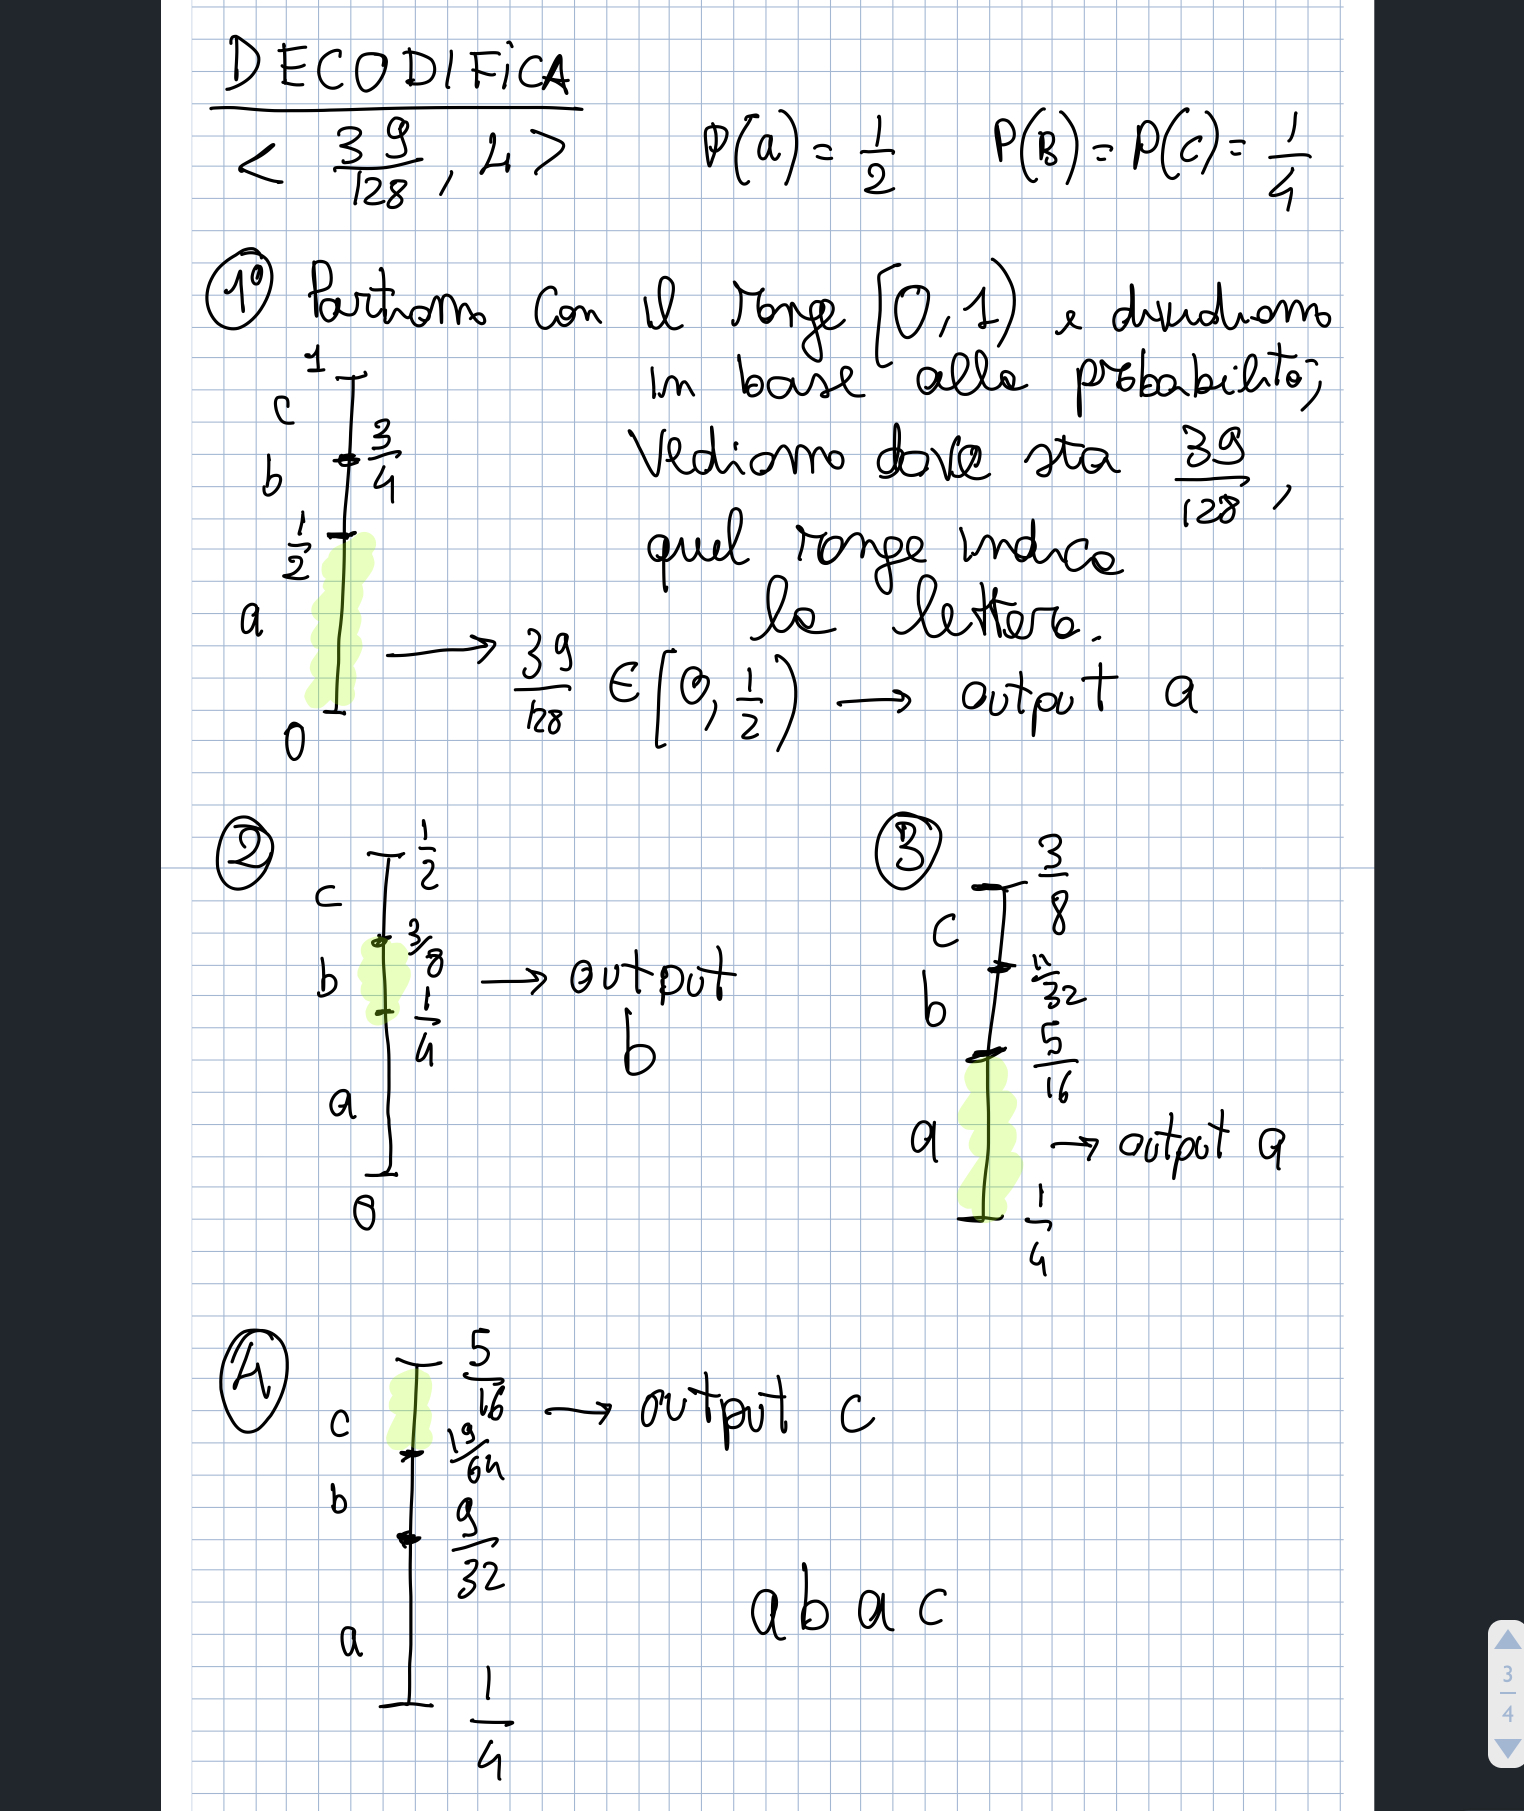
\includegraphics[width=\linewidth]{IMG_0177.jpg}
\end{figure}


\section{Efficienza di Arithmetic Coding}

La dimensione della sn finale dipende dalla probabilità dei vari caratteri della sequenza da codificare.
$sn=1*\prod^n_{i=1} P[S[i]]$.

Una volta che abbiamo fatto la codifica otteniamo un intervallo $[l_n,l_n+s_n)$ e per emettere la sequenza di bit dobbiamo trovare un intero all'interno di questo range che possa essere espresso come una frazione diadica.
Per farlo c'è da considerare un lemma:\\

Lemma: prendiamo un numero $x=0.b_1b_2...$ e consideriamo solamente i primi d bit, quindi $trunc_d(x) \in [x-2^{-d},x)$. \\
Dimostrazione: Il numero iniziale x ha in comunque con $trunc_d(x)$ i primi d bit, il resto è diverso, quindi abbiamo:\\
$x-trunc_d(x) = \sum^\infty_{i=1} b_{d+1}*2^{d-i} \leq \sum^\infty_{i=1} 1*2^{d-i} = 2^d \sum^\infty_{i=1} \frac{1}{2^i}= 2^{-d}$.

Quindi $x-trunc_d(x) \leq 2^-d$ ovvero $x-2^-d \leq trunc_d(x)$.

Da questo lemma deriva il fatto che se noi prendiamo $l_n+\frac{s_n}{2}$ come intero nel range e poi tronchiamo i primi $Log_2 \frac{2}{s_n}$ bit allora cadiamo con il numero reale scelto nell'intervallo $l_n, l_n+s_n$.\\

\textbf{Teorema:} Il numero di bit che vengono emessi dall'Arithmetic Coding per una sequenza S di lunghezza n è al più $2+nH_0$. \\
Dimostrazione: sappiamo che il numero di bit in output è pari a: \\

$Log_2 \frac{2}{s_n} < 2 - Log_2 sn = 2 - log_2(\prod^n_{i=1}P[S[i]]) = 2-\sum^n_{i=1}Log_2 P[S[i]]$

Se consideriamo $n_\sigma$ il numero di volte che un simbolo $\sigma$ occorre in S allora possiamo indicare $P[\sigma] = \frac{n_\sigma}{n}$.\\
Quindi abbiamo:
$2-\sum^n_{i=1}n_\sigma Log_2 P[\sigma]\ =\ 2-n(\sum_{\sigma \in \Sigma}P[\sigma]Log_2P[\sigma]) = 2+nH_0$. 


\chapter{Dictionary Based Compressor}

Esistono altri tipi di algoritmi di compressione oltre a quelli basati sulla statistica che sfruttano la probabilità dei vari caratteri presenti nella stringa. Ci sono gli algoritmi basati su dizionari di stringhe, presa la stringa S da codificare guardiamo all'interno del dizionario per sostituire con un token le sottostringhe di S.

\section{LZ77}

L'algoritmo di compressione LZ77 si basa su una "sliding windows" di dimensione W che contiene parte della stringa di input. L'algoritmo funziona in modo induttivo, quando arrivo alla posizione i della stringa S, suppongo di aver già compresso i precedenti i-1 caratteri.
L'algoritmo comprende una prima fase di parsing in cui vengono codificate le sottostringhe di S e una seconda fase in cui questa codifica viene trasformata in uno stream di bit con metodi come Huffman.
Il funzionamento della fase di parsing è il seguente: \\
Ci troviamo in posizione i nella stringa S, cerchiamo la sottostringa $\alpha$ che parte da i, a sinistra di i. 
Quindi mi sposto verso sinistra di $d$ caratteri e quando trovo una sottostringa in W che match $\alpha$ emetto una tripla $<d, |\alpha|, c$ dove c è il primo carattere della stringa che ha un mismatch.
La sottostringa $\alpha$ ha una dimensione variabile che dipende dalla dimensione della sottostringa che matcha e che trovo nella sliding window W.
È importante notare che $d$ può essere minore di $|\alpha|$ e quindi potremmo avere un overlap tra la stringa che vogliamo codificare e la stringa che abbiamo in W.

In LZ77 più aumenta la dimensione della sliding window e più abbiamo una compressione ma allo stesso tempo aumenta il tempo per comprimere e per decomprimere.
Diminuendo la dimensione diminuisce anche il tempo ma diminuisce anche il compression ratio.

\subsection{LZSS}

Una versione modificata di LZ77 è LZSS, la differenza è che in questo caso non viene emessa una tripla come output ma viene emessa una coppia, questa viene creata in questo modo:
\begin{itemize}
\item $<d, |\alpha|, c$ dove d è 0 e $|\alpha|$ è 0 diventa $<0,c>$
\item $<d, |\alpha|, c$ dove d e $|\alpha|$ sono diversi da 0 diventa $<d, |\alpha|$ perchè in questo modo sappiamo comunque che devo andare  sinistra di d e poi copiare una stringa di lunghezza $|\alpha|$, non ho bisogno del carattere.
\end{itemize}

\subsection{Gzip}

Gzip è una delle implementazioni di LZ77 che permette una ricerca rapida della stringa all'interno dello sliding window.
Gzip utilizza una struttura dati ausiliaria per memorizzare le varie sottostringhe che trova all'interno della stringa S.
Si utilizza una tabella hash inizialmente vuota, poi si effettuano i seguenti passaggi:
\begin{itemize}
\item Creo un blocco B di tre lettere, controllo se è presente nell'hash table e se non è presente lo inserisco e in output mando $<0,B[1]>$, poi avanzo di un carattere e creo un altro blocco di tre lettere. È possibile che alcuni blocchi siano ripetuti, in questo caso associo ad ogni blocco nella tabella la posizione in cui inizia quello specifico blocco
\item Quando trovo un blocco B già esistente nell'hash table, prendo le varie posizioni in cui si trova quel blocco e vado a confrontare B con le sottostringhe che partono da quelle posizioni. Alla fine trovo il blocco che ha in comune il prefisso più lungo con il mio e quindi trovo la posizione in cui ho il primo mismatch. 
\item Alla fine emetto la coppia $p-i*, |\alpha|$ dove p è la posizione in cui ho il mismatch e $i*$ è la posizione del blocco del dizionario che ho preso in considerazione e con cui ho il longest common prefix.
\end{itemize}

In questo caso più aumento la dimensione dei k-gram che creo e che metto all'interno del dizionario e più diminuiscono le collisioni e quindi diminuiscono anche le ricerche che vengono effettuate per trovare il longest common prefix. Invece diminuendo la k aumentano le collisioni e quindi anche le ricerche.

\subsection{Implementazione di LZ77 con il Suffix Tree}

Vogliamo eseguire la fase di Parsing di LZ77 in $O(n)$, questa fase si può effettuare utilizzando una struttura dati come il Suffix Tree in modo da mandare in output la solita tripla $d,l,T[i+l]$.
Noi in LZ77 ci troviamo in una posizione i e dobbiamo trovare una posizione $i-d$ tale che $suff_i$ e $suff_{i-d}$ abbiano in comune un prefisso $\Pi_i$ di lunghezza l.
Per trovare il suffisso di posizione $j=i-d$ però non possiamo fare una visita del suffix tree ma bisogna trovare un modo più intelligente:
\begin{itemize}
\item Si deve creare il suffix tree per la stringa da codificare
\item Facciamo una visita del suffix tree e per ogni nodo mettiamo come valore il valore minimo che troviamo nelle foglie sotto
\item Ora quando dobbiamo cercare un certo $suff_i$ iniziamo la ricerca nel suffix tree e ci fermiamo nel nodo v tale che il valore del nodo v è uguale al valore di i.
\item Dato u, il padre di v, prendiamo $s[u]$ che è la stringa in comune. In output mandiamo $<d=i-min(u), l, T[i+l]>$ dove l è la lunghezza della stringa in comune $s[u]$.
\end{itemize}

Un esempio:

\begin{figure}[H]
\centering
  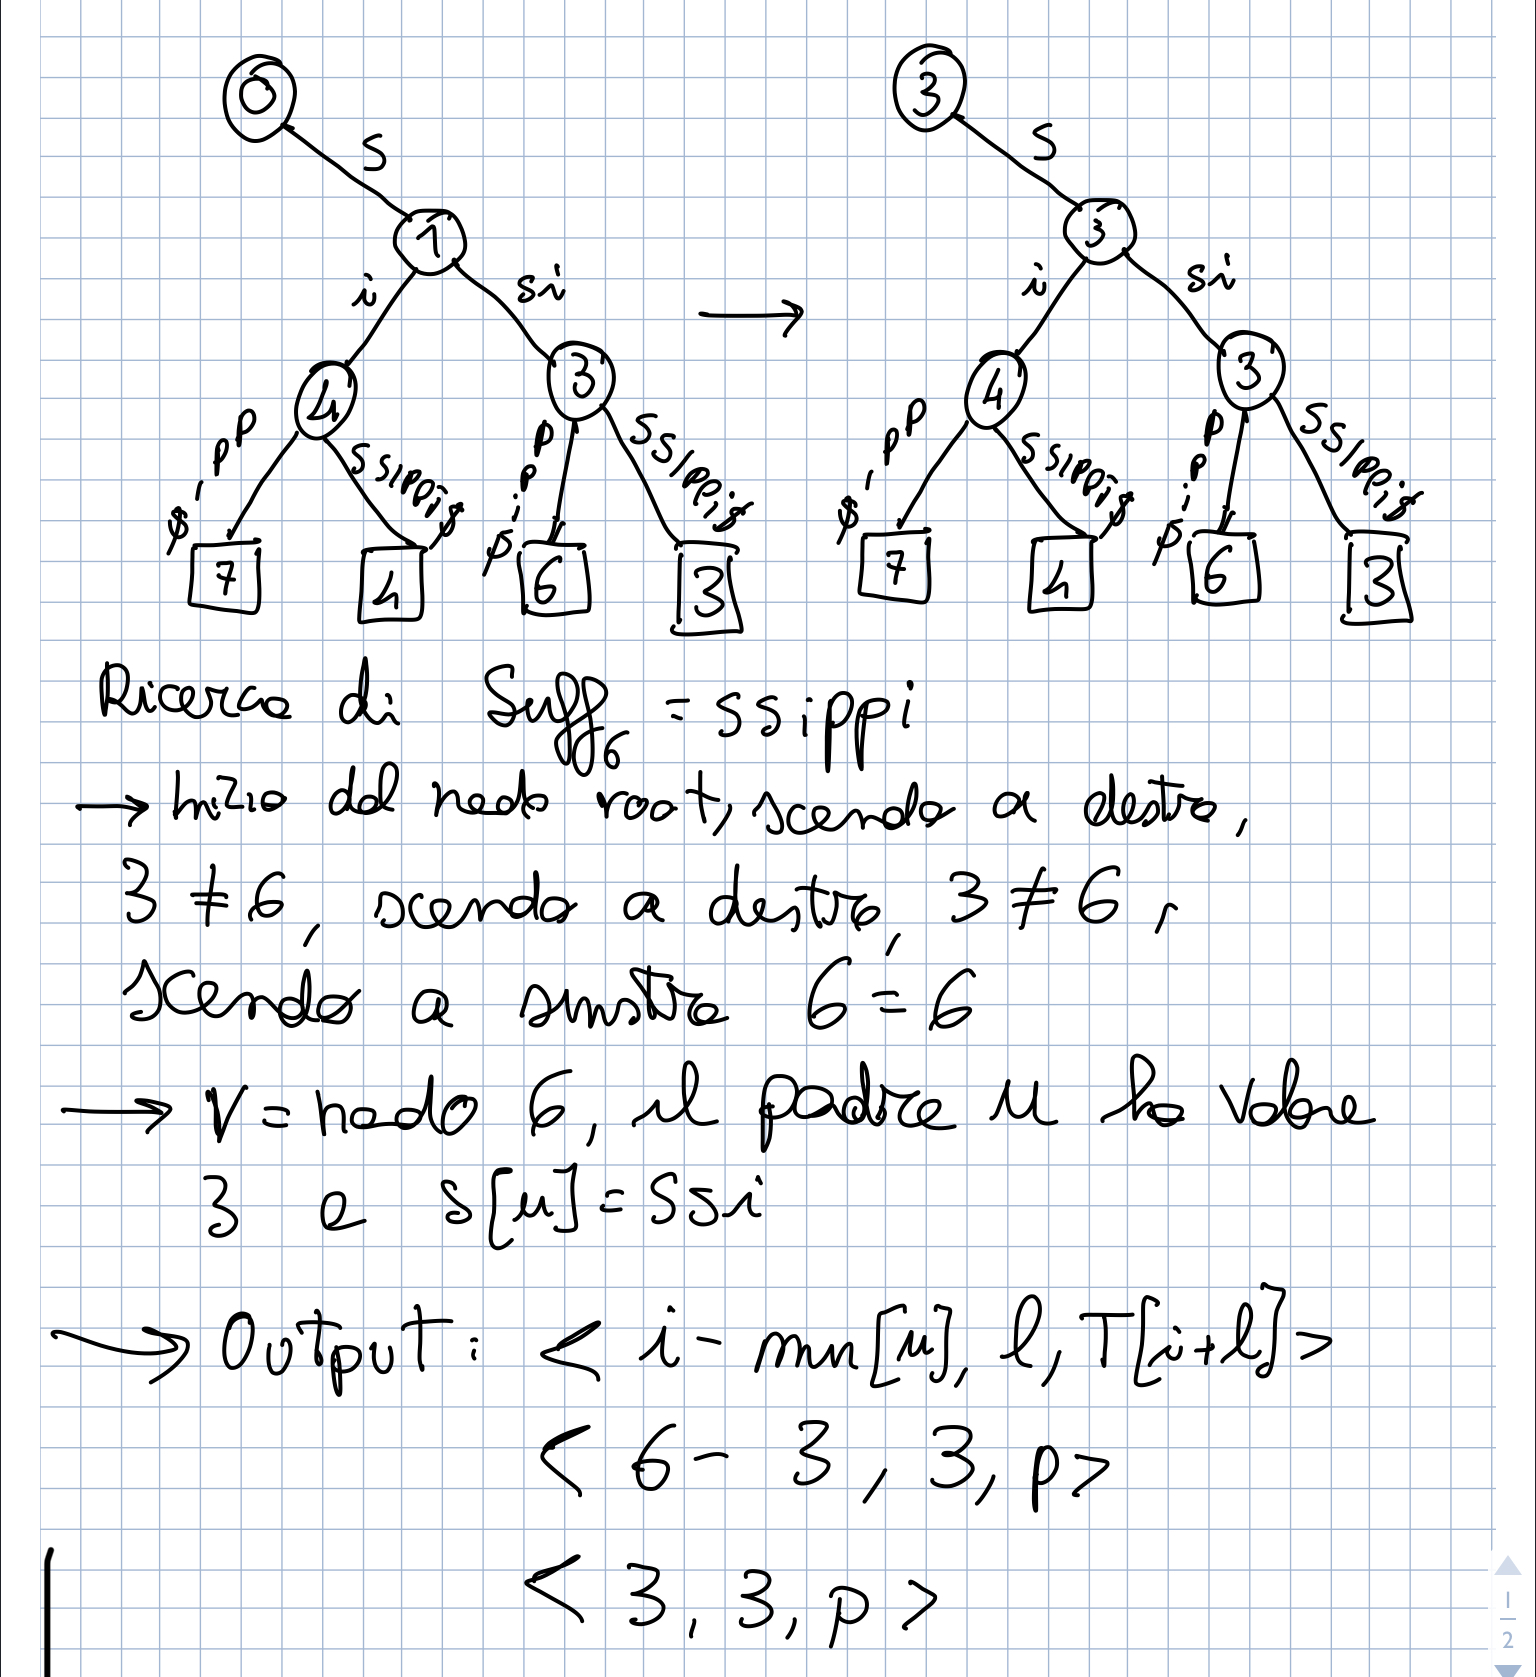
\includegraphics[width=\linewidth]{IMG_0178.jpg}
\end{figure}

\section{LZ78}

Si tratta di una evoluzione di LZ77 che cerca di risolvere il problema della sliding windows e del compression rate.
L'idea è di creare un dizionario in modo incrementale quando troviamo una nuova sottostringa da codificare.
L'algoritmo funziona in questo modo:
\begin{itemize}
\item Viene creato un dizionario che inizialmente è vuoto
\item Ammesso di essere arrivati alla posizione i della stringa e quindi di aver codificato fino a quel punto, cerchiamo la sottostringa di S che parte dalla posizione i e che è presente nel dizionario. Quando troviamo la sottostringa di lunghezza massima che è presente nel dizionario, emettiamo in output una coppia che è formata dal'ID della stringa trovata nel dizionario e dal primo carattere che segue la stringa $<ID, next_char>$. 
\item Poi inseriamo nel dizionario una nuova entry che è uguale a quella che abbiamo trovato con l'aggiunta, in fondo, del $next_char$. Anche questo nuovo elemento prende un nuovo ID.
\end{itemize}

La struttura dati che viene utilizzata per mantenere questi dati è un uncompacted trie in cui inseriamo in ogni nodo la coppia $<ID, next_char>$. 
Tramite la sequenza codificata possiamo ricostruire la stringa S di partenza e anche l'uncompacted trie.


Il problema rimane per quel che riguarda le stringhe molto grandi, in questo caso c'è il rischio di creare un dizionario enorme, quindi ci sono tre possibilità:
\begin{itemize}
\item Ad un certo punto non aggiungiamo altro nel dizionario
\item Ogni tanto svuotiamo il dizionario e ne creiamo uno nuovo
\item Per ogni inserimento eliminiamo l'elemento usato meno recentemente nel dizionario.
\end{itemize}


\chapter{Dictionary Problem}

Vogliamo avere una struttura dati che mi permetta di mantenere memorizzate delle coppie $<key, value>$ e che supporti le seguenti operazioni:
\begin{itemize}
\item Ricerca di una chiave k
\item Inserimento di una coppia $<key, value>$
\item Cancellazione di una coppia $<key, value>$
\end{itemize}

Una soluzione per questo problema potrebbe essere una tabella as accesso diretto in cui inseriamo per ogni chiave un valore. Il problema in questo caso è che avendo una grande quantità di chiavi da inserire, andremmo ad occupare molto posto.

\subsection{Hashing}

L'alternativa è utilizzare un array e una funzione hash h che, presa una chiave k vada a mappare k in una delle m posizioni dell'array.
Le varie posizioni dell'array o valgono NULL oppure hanno un puntatore ad una lista, all'interno della lista vengono inseriti i valori.
L'inserimento in questo caso ha un costo $O(1)$ perchè viene calcolata la funzione hash e poi si segue il puntatore e si inserisce il valore corrispondente all'inizio della lista.
La ricerca e la cancellazione invece hanno un costo che dipende dalla lunghezza della lista che dobbiamo scorrere per trovare l'elemento da cancellare.
Nel caso in cui dovessimo avere una funzione h capace di distribuire in modo random tutte le chiavi ovvero una funzione "uniform hash" allora ci troveremmo con m possibili bucket nella tabella hash e n inserimenti da fare, in questo caso avremmo liste di dimensione $\frac{n}{m}$ perchè ogni elemento ha probabilità $\frac{1}{m}$ di finire nei vari bucket. La $\frac{n}{m}$ è detto load factor.
Lo spazio occupato da una tabella hash di questo tipo è $O(n+m)Log_2n + n(Log_2 u)$ bit.

Il problema è che h semplice e uniforme non esiste nella realtà perchè anche se abbiamo una funzione di questo genere possiamo mappare alcuni valori tutti in un unico bucket. Va fatta una distinzione tra hash function e famiglie di hash function.

Due possibili metodi per creare una buona hash function:
\begin{itemize}
\item Hashing con divisione: la funzione hash viene calcolata come resto della divisione di k con la dimensione m della tabella: $h(k)=k\ mod\ m$.
\item Hashing con moltiplicazione: in questo caso abbiamo $h(k)=m\ frac(kA)$.
\end{itemize}

\section{Universal Hashing}

Non abbiamo una funzione hash semplice ed uniforme.
Se abbiamo U key da mappare in ${0,1,...,m-1}$ interi abbiamo un numero di funzioni hash pari a $m^{|U|}$, questo comporta la necessità di $ULog_2m$ bit per rappresentare una delle funzioni.
Dato che serve troppo spazio per rappresentare questa funzione hash, questo percorso non è fattibile.

L'idea quindi è quella di usare una strategia differente e prendere le funzioni hash da una famiglia di funzioni a random un po' come si fa quando si prende il pivot del quicksort.

\textbf{Universal Hashing: } Data H collezione finita di hash function che mappa un universo U in interi ${0,1...m-1}$ allora H è universale se e solo se \\
\begin{equation}
|{h \in H: h(x) = h(y)}| \leq \frac{|H|}{m}
\end{equation}

Questo mi dice anche che la probabilità di avere $P(h(x)=h(y))$ sarà uguale a $\frac{\frac{|H|}{m}}{|H|}$ ovvero $\frac{1}{m}$.

\textbf{Teorema: } Data l'hash table con chaining, la lunghezza media delle liste che si creano è pari a $1+\frac{n}{m}$ dove m è la dimensione dell'hash table e n sono gli elementi inseriti all'interno.

\textbf{Dimostrazione: } Per prima cosa definiamo $I_{x,y}$: \\

$I_{x,y}$:
\begin{cases}
      1, & \text{if}\ h(x)=h(y) \\
      0, & \text{otherwise}
    \end{cases}

Ora consideriamo che la $P(h(x)=h(y)) < \frac{1}{m}$ e quindi abbiamo che 
\begin{equation}
E[I_{x,y}] = 1*P(I_{x,y}=1) + 0* P(I_{x,y}=0) = P(I_{x,y}=1) \leq \frac{1}{m}
\end{equation}

Ora calcoliamo $N_x$ che mi indica il numero di chiavi che collidono con x, escluso x:
\begin{equation}
N_x = \sum_{y \in D} E[I_{x,y}] = \sum_{y \in D} P(I_{x,y}=1) = \frac{n-1}{m} \leq \frac{n}{m}
\end{equation}

Se consideriamo anche x abbiamo la dimostrazione.

\subsection{Definizione della Universal Hash Function}

Vogliamo creare una famiglia di universal hash Fuction tale che $H = {h:\ U\ ->\ {0,...,m-1}}$. Le chiavi sono rappresentate con $Log_2 U $ bit e la tabella ha dimensione m.
Definiamo $r=\frac{Log_2 |U|}{Log_2 m}$, e decomprimiamo ogni chiave k in $[k_0,k_1,....,k_{r-1}]$, ogni parte della chiave è formata al più da $log_2 m$ bit. La stessa cosa la facciamo con un intero a quindi abbiamo $[a_0,a_1,....,a_{r-1}]$.

\textbf{Teorema: } la classe H che contiene le funzioni definite come $h_a(k)\ =\ \sum^{r-1}_{i=0}a_ik_i\ mod\ m$ con m primo e a intero positivo è universale.

\textbf{Dimostrazione: } Prendiamo due interi x e y che sono diversi per almeno un bit, $x_0 \neq y_0$. 
Ora vogliamo dimostrare che il numero di collisioni è limitato da $\frac{|H|}{m}$ e quindi che abbiamo H universale.
\begin{equation}
h_a(x) = h_a(y) ==> \sum^{r-1}_{i=0} a_i*x_i mod m = \sum^{r-1}_{i=0} a_i*y_i mod m 
\end{equation}
\begin{equation}
 (a_0*x_0)\sum^{r-1}_{i=1} a_i*x_i mod m = (a_0*y_0)\sum^{r-1}_{i=1} a_i*y_i mod m
\end{equation}

\begin{equation}
a_0(x_0-y_0) = \sum^{r-1}_{i=1} a_i*(x_i-y_i) mod m
\end{equation}

\begin{equation}
a_0 = (\sum^{r-1}_{i=1} a_i*(x_i-y_i))*(x_0-y_0)^{-1} mod m
\end{equation}

Ora possiamo dire che $(x_0-y_0)^{-1}$ esiste ed è un intero compreso tra $[0,|U|-1]$, quindi abbiamo trovato l'unico valore di $a_0$ per cui abbiamo una collisione. Allo stesso modo possiamo fare la stessa cosa per le altre $[a_1,....,a_{r-1}]$, quindi in tutto abbiamo $m^{r-1}$ collisioni e quindi 
\begin{equation}
m^{r-1} = \frac{|U|}{m} = \frac{|H|}{m}
\end{equation}

\section{Perfect, Minimal e Order Preserving Hashing}

\textbf{Definizione:} Una funzione hash $h:\ U->{0,1,...,m-1}$ si dice perfetta se per ogni coppia $x,y$ abbiamo che $h(x) \neq h(y)$. 

\textbf{Definizione:} Una funzione hash si dice perfetta se data la dimensione m della tabella e la dimensione n del dizionario di elementi da inserire nella tabella, abbiamo che $m=n$. Ovvero se abbiamo un elemento per ciascun bucket.

\textbf{Definizione:} Una funzione hash si dice preserving order se prese due chiavi $k_0$ e $k_1$ con $k_0\ <\ k_1$ abbiamo che $h(k_0)\ <\ h(k_1)$.

Vogliamo creare una funzione h che abbia tutte queste caratteristiche, presa la tabella di dimensione m e la dimensione n del dizionario, ci servono delle funzioni ausiliarie:
\begin{itemize}
\item Ci serve una funzione hash $h_1$ e una funzione hash $h_2$ che mappano le stringhe che dobbiamo inserire nella hash table in interi compresi nell'intervallo $[0,m-1]$.
\item Ci serve una funzione g che mappa gli interi da $[0,m-1]$ a $[0,n-1]$
\end{itemize}

La nostra funzione hash alla fine sarà definita come $h(t)=(g(h_1(t)) + g(h_2(t))) mod\ m$.

Ora, le due funzioni hash $h_1$ e $h_2$ sono prese random dalla classe U di funzioni possibili, invece la funzione $g$ è diversa e la possiamo costruire in un certo modo.

Come costruire la funzione $g$:
\begin{itemize}
\item Dobbiamo creare un grafo aciclico che ha un numero di nodi pari alla dimensione m.
\item Per ogni elemento da inserire nella hash table calcoliamo $h_1$ e $h_2$ e poi uniamo i nodi corrispondenti ai valori calcolati.
\item Gli archi vengono labellati in ordine crescente in base a quando vengono aggiunti.
\item Per ottenere g dobbiamo fare una visita di questi nodi, partiamo da uno qualsiasi e per calcolare g(i) dobbiamo calcolare $g(v_i)=(h(v_{i-1},v_i)-g(v_{i-1}))mod\ n$.
Ad ogni nodo seguiamo gli archi e ricorsivamente calcoliamo il valore di g. Quando ci fermiamo perchè non ha più vicini cambiamo nodo.
\end{itemize}

È importante che il grafo sia aciclico altrimenti non trovo soluzioni.
Se il grafo non è aciclico devo renderlo tale andando a spostare l'arco che lo rende ciclico e collegandolo ad un altro nodo.

Un esempio di questa procedura:

\begin{figure}[H]
\centering
  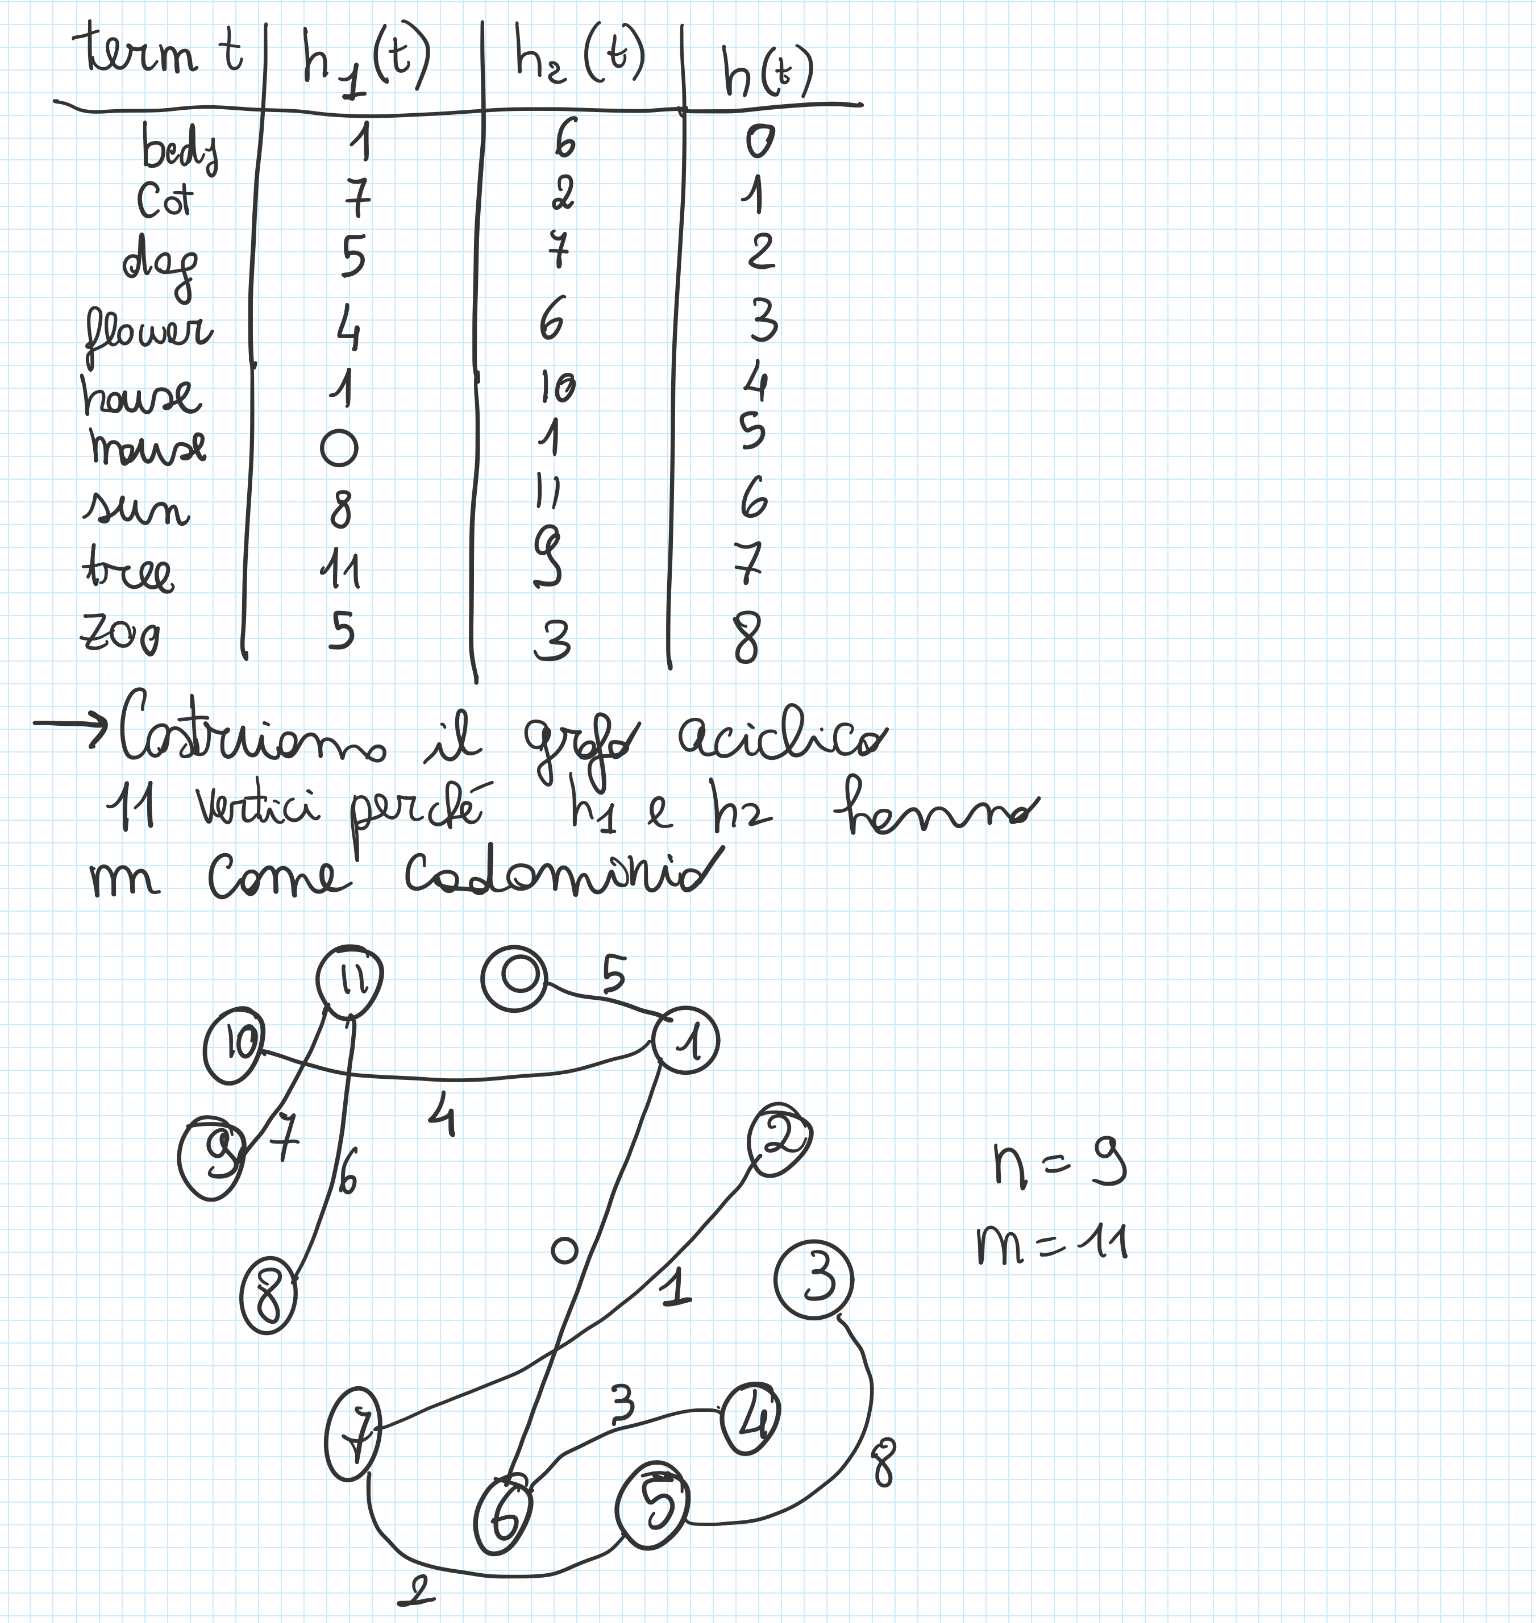
\includegraphics[width=0.8\linewidth]{IMG_0188.jpg}
\end{figure}

\begin{figure}[H]
\centering
  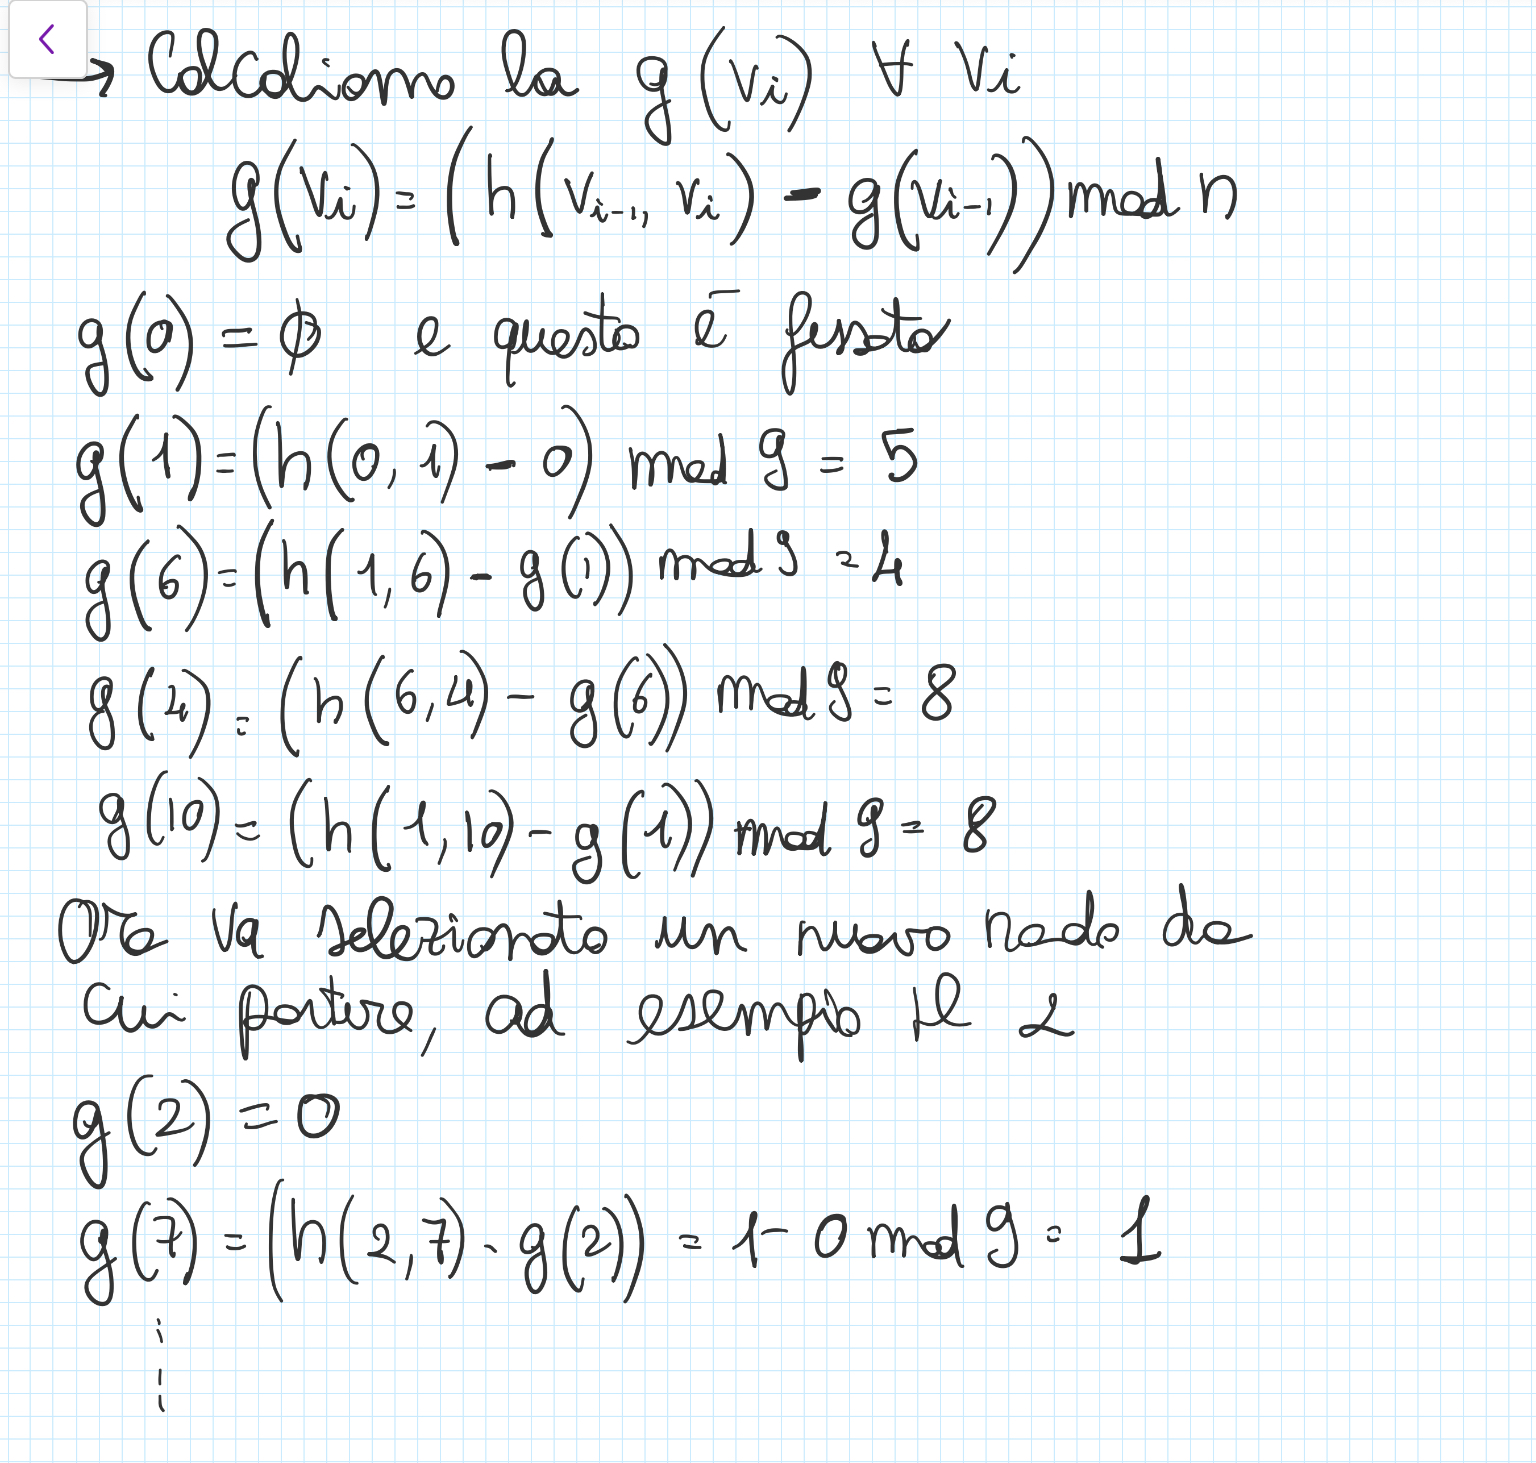
\includegraphics[width=0.8\linewidth]{IMG_0189.jpg}
\end{figure}


\section{Costruire l'hash table perfetta}

Se vogliamo una hash table che sia perfetta (e non minimal e preserving order) possiamo utilizzare un two level hashing scheme. 
In questo metodo andiamo ad utilizzare una prima hash table di dimensione m in cui inseriamo n elementi, al momento dell'inserimento però non creiamo la lista per ogni key, ogni bucket punterà ad una seconda tabella hash che avrà una sua corrispondente funzione hash che deve fare in modo di non creare collisioni tra gli elementi che vengono inseriti all'interno.

\textbf{Teorema:} Data una hash table di dimensione $q^2$ e $q$ chiavi da inserire all'interno dell'hash table, allora abbiamo un numero di collisioni atteso pari a $\frac{1}{2}$. Quindi la probabilità di collisioni p pari a $\frac{1}{2}$.

\textbf{Dimostrazione:} Dato che abbiamo $q$ chiavi da inserire all'interno dell hash table, consideriamo le possibili coppie che possiamo creare, queste sono $\binom{q}{2}$. 
Se consideriamo che per definizione di hash function ogni coppia ha probabilità $\frac{1}{m}$ di avere una collisione, possiamo scrivere:

\begin{equation}
\binom{q}{2}*\frac{1}{m} = \binom{q}{2}*\frac{1}{q^2} = \frac{q(q-1)}{2}*\frac{1}{q^2} < \frac{q^2}{2q^2} = \frac{1}{2}
\end{equation}

Ora possiamo considerare lo spazio occupato dalla struttura dati in due livelli che utilizziamo per risolvere il problema.

\textbf{Teorema:} Se inseriamo n chiavi in una tabella hash di dimensione $m=n$ allora la dimensione complessiva delle sotto tabelle che vengono create per memorizzare le n chiavi è pari a $E[\sum^{m-1}_{j=0}n_j^2]\ <\ 2n$.

\textbf{Dimostrazione:} Consideriamo:

\begin{equation}
E[\sum^{m-1}_{j=0}n_j^2] = E[\sum^{m-1}_{j=0}(n_j + 2\binom{n_j}{2})] = E[\sum^{m-1}_{j=0}(n_j) + 2\sum^{m-1}_{j=0}\binom{n_j}{2})] = n + E[2\sum^{m-1}_{j=0}\binom{n_j}{2}]
\end{equation}

Ora consideriamo che $2\sum^{m-1}_{j=0}\binom{n_j}{2}$ indica il numero delle collisioni create da h, dato che abbiamo una universal hash function possiamo dire che questo è pari a $\binom{n}{2}\frac{1}{m}$. Quindi abbiamo 
\begin{equation}
n + 2\binom{n}{2}\frac{1}{m} = n + 2\frac{n(n-1)}{2}\frac{1}{m} = 2n-1 < 2n
\end{equation}

Quindi in ognuna delle tabelle hash aggiuntive che vengono create ci stanno al più $2n$ elementi.



\section{Cuckoo Hashing}

Quando dobbiamo utilizzare un dizionario dinamico allora bisogna utilizzare il Cuckoo Hashing per la creazione della tabella hash.
Il Cuckoo Hashing ci consente di:
\begin{itemize}
\item Effettuare ricerche in tempo costante
\item Effettuare cancellazioni in tempo costante
\item Effettuare inserimenti in tempo costante, anche se per gli inserimenti consideriamo che ogni tanto potremmo dover fare una operazione più costosa che poi ammortizziamo con il passare del tempo e inserendo nuove chiavi nel dizionario
\end{itemize}


Come funziona il Cuckoo Hashing:

\begin{itemize}
\item Scegliamo due funzioni hash, $h_1(x)$ e $h_2(x)$
\item Per ogni chiave che viene inserita calcoliamo $h_1(x)$ e $h_2(x)$ e abbiamo varie possibili situazioni:
\begin{itemize}
\item La posizione $h_1(x)$ o $h_2(x)$ è libera, in questo caso inseriamo senza problemi e creiamo un arco tra $h_1(x)$ e $h_2(x)$.
\item Entrambe le posizioni sono occupate, in questo caso dobbiamo spostare uno degli elementi e lo spostiamo nella posizione a cui è collegato e poi facciamo l'inserimento del nuovo valore.
\end{itemize}
\end{itemize}


Il problema ce l'abbiamo quando spostiamo una chiave già esistente perchè in alcuni casi possono crearsi dei cicli che possono fermare l'algoritmo. In questi casi l'unica cosa è effettuare il re hashing modificando la funzione hash e cambiando quindi la disposizione degli elementi all'interno della tabella. Il costo $O(n)$ del re hashing è ammortizzato dall'inserimento in $O(1)$ che viene fatto.

\textbf{Teorema:} Per ogni coppia i,j di posizioni nella tabella, con $m\geq 2cn$ dove m è la dimensione della tabella e n sono le chiavi nel dizionario, abbiamo che la probabilità che esista un percorso da i a j di lunghezza $L \geq 1$ è al più $\frac{c^-L}{m}$. 

\textbf{Dimostrazione:} La dimostrazione è per induzione:
\begin{itemize}
\item Per L=1 dobbiamo calcolare la probabilità di avere un arco che collega i a j. Abbiamo $\frac{1}{m}$ di probabilità di avere una chiave che finisce in i e $\frac{1}{m}$ che finisca in j, va moltiplicato per 2 perchè abbiamo 2 funzioni hash per ogni chiave. Ora consideriamo anche il fatto di avere n possibili chiavi e quindi possiamo calcolare la probabilità per il caso L=1. Abbiamo quindi $\sum_{n \in S}\frac{2}{m^2} = \frac{2n}{m^2}$. Dato che abbiamo $m\geq 2n$ allora $\frac{m}{c}\geq 2n$ quindi:
\begin{equation}
\frac{2n}{m^2} = \frac{mc^-1}{m^2} = \frac{c^-1}{m}
\end{equation}

\item Prendiamo poi il caso $L\geq1$, sappiamo che il teorema vale fino a L-1 e consideriamo una divisione del path che va da i a j:
\begin{itemize}
\item Una prima parte del percorso va da i a z ed è lungo L-1, questo ha una probabilità che è limitata da $\frac{c^{-L+1}}{m}$
\item Una seconda parte va da z a j ed abbiamo probabilità $\frac{c^{-1}}{m}$. 
\end{itemize}
Ora moltiplichiamo le due probabilità quindi otteniamo $\frac{c^{-L+1}}{m}*\frac{c^{-1}}{m}$ ovvero $\frac{c^{-L}}{m^2}$. Se consideriamo le possibili m posizioni che può prendere z allora abbiamo $\frac{c^{-L}}{m}$
\end{itemize}


\textbf{Teorema:} Per ogni coppia di chiavi x,y abbiamo che la probabilità che x venga hashato nella stessa posizione di y è $O(\frac{1}{m})$.

\textbf{Dimostrazione:} Consideriamo la probabilità che si crei un ciclo di una lunghezza L ovvero la probabilità di avere un arco che parte dalla posizione i e arriva in i. Consideriamo che stando al teorema precedente questo avviene con probabilità $\frac{c^{-L}}{m}$. 
Se consideriamo tutte le possibili L abbiamo:
\begin{equation}
\sum^{\infty}_{L=0}\frac{c^{-L}}{m} = \frac{1}{m}\sum^{\infty}_{L=0}\frac{1}{C^L} = \frac{1}{m}*\frac{1}{c-1}
\end{equation}

Quindi è $O(m)$.

\textit{Corollario:} Fissando $c\geq3$ e prendendo $m\geq6n(1+\epsilon)$ allora possiamo dire che la probabilità di avere un ciclo nel grafo è minore di $\frac{1}{2}$.


\section{Bloom Filter}

Ci sono alcune situazioni in cui non è possibile memorizzare le chiavi all'interno di una hash table ma vorremmo comunque capire se una certa chiave è presente o meno. Un esempio può essere quello di un crawler di pagine web che deve memorizzare i link alle pagine visitate. Mantenere tutti i vari link sarebbe uno spreco di memoria quindi si preferisce usare il bloom filter.

Il funzionamento del bloom filter è abbastanza semplice:
\begin{itemize}
\item Abbiamo r funzioni hash $h_0,...h_{r-1}$
\item Abbiamo un array di bit di dimensione m
\item Abbiamo n chiavi da inserire
\end{itemize}

Per ogni chiave che deve essere inserita calcoliamo r volte l'hash utilizzando le r funzioni e settiamo a 1 il bit corrispondente.
Una volta che dobbiamo fare una ricerca ci sono due situazioni:
\begin{itemize}
\item La ricerca ci porta a trovare un $B[i]=0$, in questo caso possiamo dire con sicurezza che quella chiave non è presente all'interno dell'array di bit
\item Se invece abbiamo per tutte le funzioni hash $B[i]=1$ allora possiamo dire che:
\begin{itemize}
\item La chiave è effettivamente presente all'interno del bloom filter
\item La chiave non è presente ma comunque viene restituito si e quindi abbiamo un falso positivo.
\end{itemize}
\end{itemize}

Vogliamo cercare di capire il valore della probabilità di avere un falso positivo.
Per prima cosa consideriamo il caso in cui inseriamo una chiave, vogliamo vedere, dopo ogni inserimento, la probabilità che una certa posizione i rimanga a 0.
\begin{equation}
P(B[i]=0 dopo un inserimento) = (\frac{m-1}{m})^r
\end{equation}

Ora consideriamo che facciamo n inserimenti quindi questa probabilità diventa:
\begin{equation}
P(B[i]=0 dopo n inserimenti) = (\frac{m-1}{m})^rn = (e^{-\frac{rn}{m}})
\end{equation}

Ora consideriamo la probabilità che con x non appartenente al dizionario, venga comunque data una risposta positiva:

\begin{equation}
P(falso\ positivo) = P(1-e^{-\frac{rn}{m}})^r = (0.6185)^{\frac{m}
{n}}
\end{equation}


È importante scegliere un valore di r che sia sensato e che permetta di abbassare al minimo la probabilità di falsi positivi.
Per calcolare il valore di r che vogliamo utilizzare:
\begin{equation}
k_{opt}=\frac{m}{n}Ln 2
\end{equation}

Lo spazio occupato dal bloom filter è pari a: $1.44*n*Log_2\frac{1}{\epsilon}$ bit ovvero è lontano solamente per la costante 1.44 dall'ottimo.


\chapter{Treaps e Skip List}

\section{Treaps}

Un treap è una struttura ad albero in cui ogni nodo contiene due informazioni, una chiave per la ricerca e un valore che indica la priorità. I nodi sono ordinati come se fosse un albero binario di ricerca in base alla chiave, allo stesso tempo però sono ordinati in base alla priorità come se fosse un Min Heap.
Quindi, dato un nodo dobbiamo rispettare alcune regole:
\begin{itemize}
\item Gli elementi a sinistra sono tutti minori dal punto di vista del valore e quelli a destra sono tutti maggiori
\item Andando verso il basso diminuisce il valore della priorità dei vari nodi.
\end{itemize}

Ogni nodo poi ricorsivamente è un treap e quindi valgono le due proprietà.

\subsection

Le operazioni che possiamo svolgere su un treap sono le classiche degli alberi, abbiamo la all'interno dell'albero che è l'operazione più semplice.

Per inserire un nuovo elemento all'interno dell'albero invece dobbiamo svolgere una operazione un po' più complessa:
\begin{itemize}
\item Il nuovo elemento viene inserito in fondo all'albero come avviene con gli alberi binari di ricerca
\item La proprietà dello heap in questo modo potrebbe non essere più valida quindi è necessario modificare l'albero.
\item Viene effettuata una operazione chiamata rotazione che costa $O(1)$ perchè è solamente uno scambio di puntatori, questa mi permette di andare a modificare l'ordine dei nodi e quindi di ottenere un treap che rispetti anche la proprietà dello heap.
\end{itemize} 

Eliminare un nodo invece è simile all'aggiunta, una volta selezionato il nodo da eliminare andiamo a fissare come $+\infty$ la sua priorità e quindi con varie rotazioni portiamo il nodo in fondo all'albero.
Alla fine dato che il nodo è diventato una foglia, riusciamo a cancellarlo.
Un'altra operazione che possiamo effettuare è lo split del treap in un certo nodo. Una volta selezionato il nodo dobbiamo fissare la sua priorità a $-\infty$ (se il pivot su cui vogliamo splittare non esiste lo aggiungiamo), in questo modo il nodo viene portato fino al nodo root e così possiamo splittare senza problema.

Il merge di due treap invece avviene andando a inserire un nodo dummy con priorità $+\infty$, questo è il root dei due treap, poi con le rotazioni lo spostiamo in una foglia e lo eliminiamo.\\

Quindi i costi sono:

\begin{itemize}
\item Ricerca: O(depht(v))
\item Inserimento: O(depth(v))
\item Cancellazione: O(depth(v))
\item Split e Merge: O(depth(v))
\end{itemize}

\subsection{Dimostrazione che la profondità di un treap è in media $O(Log_2n)$}

\textbf{Teorema:} Se le priorità del treep sono random allora la profondità media è pari a $O(Log_2n)$.

\textbf{Dimostrazione:} Per questa dimostrazione consideriamo un set di chiavi $x_1,...,x_n$ in ordine crescente di valore.
Definiamo un altro set:

$A^i_k$ = 
\begin{cases}
      1, & \text{if}\ $x_i$ è ancestor di $x_k$ \\
      0, & \text{otherwise}
\end{cases}

Dato questo set possiamo vedere che la profondità di un nodo k la possiamo calcolare andando a vedere quanti sono i suoi ancestor.
Quindi possiamo scrivere: $depth(x_k)=\sum^{n}_{i=1}A^i_k$, se consideriamo poi la media delle varie profondità possiamo scrivere: $E[depth(x_k)]=\sum^{n}_{i=1}E[A^i_k] = \sum^{n}_{i=1}1*P(A^i_k=1)+0*P(A^i_k=0)=\sum^{n}_{i=1}P(A^i_k=1)$.

Quindi ora rimane da calcolare la probabilità che un certo nodo i sia un ancestor di un altro nodo k. 
Per definizione di ancestor, preso un nodo $x_i$ è ancestor di $x_k$ se $x_i$ è il nodo con più bassa priorità all'interno dell'intervallo $(i,k)$.
Quindi abbiamo $\frac{1}{|k-i|+1}$ probabilità di avere i come minima probabilità in quel set.\\
Quindi abbiamo: $E[depth(x_k)]=\sum^{n}_{i=1}P(A^i_k=1)=\frac{1}{|k-i|+1}$ che equivale a $O(Log_2n)$.
    
\section{Skip List}

Si tratta di un'altra struttura dati che ha una struttura differente rispetto agli alberi binari e ai treep ma che ha le stesse proprietà interessanti.
Abbiamo una lista di n elementi, in questo caso la ricerca di un certo elemento andrebbe a costare al caso pessimo $O(n)$ perchè dovremmo scorrere tutta la lista.
L'idea è quella di creare un secondo livello della lista in cui andiamo ad inserire parte degli interi che sono nella prima lista. Per ognuno degli interi lanciamo una moneta quindi abbiamo probabilità $\frac{1}{2}$ di finire nel livello successivo e $\frac{1}{2}$ di non finirci.
In questo modo la ricerca viene effettuata prima nel livello con meno elementi e poi quando troviamo un elemento che è maggiore di quello che cerchiamo allora andiamo nel primo livello e facciamo una ricerca in una parte della lista completa. Dato che ogni nodo ha probabilità $\frac{1}{2}$ di capitare nella seconda lista allora al più avremo da visitare $\frac{n}{2}$ nodi.

Ovviamente possiamo andare a creare più liste e ad ogni lista che aggiungiamo dimezziamo la quantità di interi che sono presenti all'interno.

\textBf{Teorema:} L'altezza della skip list è con alta probabilità $O(Log_2n)$.

\textBf{Dimostrazione:} Abbiamo detto che per ogni elemento della lista abbiamo $\frac{1}{2}$ di probabilità di selezionarlo e portarlo al livello successivo. Quindi se consideriamo un elemento x e vogliamo la probabilità che questo arrivi al livello l ovvero che $P(L(x)\ \geq \ l)$ dobbiamo considerare la probabilità che per almeno l volte capita testa quando lancio la moneta. Quindi abbiamo $P(L(x)\ \geq \ l) = \frac{1}{2^l}$.

Ora consideriamo che abbiamo n elementi nella lista quindi abbiamo $P(L\ \geq \ l) = \sum^n_{i=1} \frac{1}{2^l} = \frac{n}{2^l}$.
Se fissiamo $l=cLog_2n$ allora abbiamo:
\begin{equation}
P(L\ \geq \ cLog_2n) = \frac{n}{2^{cLog_2n}} = \frac{n}{n^c} = \frac{1}{n^{c-1}}
\end{equation}

Quindi l'altezza della skip list è $O(Log_2 n)$ con alta probabilità.


\end{document}

